%=============================================================================
% Threshold-Aware Initialization / The Ternary Operating Point
% FINAL SUBMISSION-READY MANUSCRIPT
% Target journal: Neurocomputing (Elsevier)
%
% ---------------------------------------------------------------------------
% COMPILATION
% ---------------------------------------------------------------------------
% TeXstudio build profile: PdfLaTeX -> BibTeX -> PdfLaTeX -> PdfLaTeX
% All four passes are required: the bibliography is external (ref.bib).
%
% Required class and packages, all present in TeX Live 2021+ / MiKTeX full:
% elsarticle, amsmath, amssymb, amsthm, algorithm2e, booktabs, array,
% graphicx, xcolor, natbib (loaded by elsarticle), hyperref, url
%
% ---------------------------------------------------------------------------
% FILES IN THIS PACKAGE
% ---------------------------------------------------------------------------
% manuscript.tex this file -- the complete manuscript
% ref.bib bibliography database, 49 entries
% elsarticle.cls Elsevier article class (bundled for portability)
% elsarticle-num.bst Elsevier numbered reference style (v2.1)
% fig1_*.png... fig10_*.png the ten figures
% Every file sits in one flat directory; there are no subfolders to configure.
%
% For the Elsevier two-column submission layout, replace the \documentclass
% line with: \documentclass[final,5p,times,twocolumn]{elsarticle}
% The single-column preprint option is used here because Algorithm 1 and
% Tables 2-3 are wide.
%
% FIGURES
% Ten PNG figures sit alongside this file:
% fig1_convergence fig2_final_loss fig3_rho0_sweep fig4_lmeval
% fig5_pareto fig6_scale fig7_h3_falsification fig8_init_ablation
% fig9_two_slope fig10_mechanism
% Edit \graphicspath if they are moved elsewhere.
%
% BIBLIOGRAPHY
% References are kept in ref.bib and typeset with elsarticle-num, the
% numbered Elsevier style Neurocomputing requires. 57 entries, all 57 cited,
% no orphans, no duplicate works, and every entry carries author, title, year
% and the venue field its type requires.
% DOI STATUS: 7 entries carry a DOI. The remainder are ICLR, NeurIPS, ICML
% (PMLR), MLSys, OpenReview or arXiv items, none of which mint DOIs, so the
% absence is correct rather than missing. Two further DOIs were located but
% rest on a single aggregator record and are therefore NOT included here:
% he2015 (10.1109/ICCV.2015.123) and zhang2018 (10.1007/978-3-030-01237-3_23).
% Confirm them against IEEE Xplore and SpringerLink before adding.
% PUBLISHED VERSIONS: hoffmann2022 appeared at NeurIPS 2022 as "An Empirical
% Analysis of Compute-Optimal Large Language Model Training" (same authors,
% changed title, no DOI). The arXiv form is retained because the title the
% text refers to is the preprint's.
%
% PROVENANCE
% Every numeric claim derives from the released research artefact
% (manifest hash 3e7a849df17d63d7): results/tai_manifest.json,
% analysis_summary.csv, results_all_runs.csv, the 3,016-record runs/ store,
% and logs/console_20260822.log.
%=============================================================================

\documentclass[final,5p,times,twocolumn]{elsarticle}
%% Neurocomputing uses NUMBERED references in square brackets, e.g. [1], [1,2],
%% [1--4]. `numbers' is the elsarticle default, so no citation option is given
%% above. \biboptions below enables author-name forms via \citet and compresses
%% consecutive numbers, matching elsarticle-template-num-names.tex.
\biboptions{numbers,sort&compress}

%% For the journal's two-column production layout, use instead:
%% \documentclass[final,5p,times,twocolumn]{elsarticle}
%% For a double-spaced, line-numbered version for referees, use:
%% \documentclass[review,11pt]{elsarticle}
%% \usepackage{lineno}\linenumbers

%% ---------------------------------------------------------------------------
%% elsarticle VERSION COMPATIBILITY SHIM
%% The keyword form \affiliation{organization=..., city=..., country=...} was
%% introduced in elsarticle v3.3. Installations shipping v3.2 (2019) or earlier
%% -- including some Editorial Manager build servers -- provide only \address,
%% and fail with Undefined control sequence at \affiliation.
%% This block is a no-op on v3.3+ and supplies a faithful \affiliation on older
%% versions. Delete it once you have confirmed the target installation is v3.3+.
%% ---------------------------------------------------------------------------
\usepackage{keyval}
\makeatletter
\@ifundefined{affiliation}{%
\define@key{elsaff}{organization}{\def\els@org{#1}}%
\define@key{elsaff}{addressline}{\def\els@line{#1}}%
\define@key{elsaff}{city}{\def\els@city{#1}}%
\define@key{elsaff}{postcode}{\def\els@post{#1}}%
\define@key{elsaff}{state}{\def\els@state{#1}}%
\define@key{elsaff}{country}{\def\els@ctry{#1}}%
\newcommand{\affiliation}[2][]{%
\def\els@org{}\def\els@line{}\def\els@city{}%
\def\els@post{}\def\els@state{}\def\els@ctry{}%
\setkeys{elsaff}{#2}%
\def\els@out{}%
\ifx\els@org\@empty\else\edef\els@out{\els@org}\fi
\ifx\els@line\@empty\else\edef\els@out{\els@out, \els@line}\fi
\ifx\els@city\@empty\else\edef\els@out{\els@out, \els@city}\fi
\ifx\els@post\@empty\else\edef\els@out{\els@out\ \els@post}\fi
\ifx\els@state\@empty\else\edef\els@out{\els@out, \els@state}\fi
\ifx\els@ctry\@empty\else\edef\els@out{\els@out, \els@ctry}\fi
\address[#1]{\els@out}%
}%
}{}
\makeatother

\usepackage[T1]{fontenc}
\usepackage[utf8]{inputenc}
\usepackage{amsmath,amssymb,amsthm}
\usepackage{booktabs}
\usepackage{array}
\usepackage{graphicx}
\usepackage{xcolor}
\usepackage[ruled,vlined,linesnumbered]{algorithm2e}
\usepackage{url}
\usepackage[hidelinks]{hyperref}
%% LaTeX's default float fractions reserve so much of each page for text that a
%% tall double-column float cannot share a page with any, which stranded
%% Table~\ref{tab:threats} on a page of its own after the conclusion. Relaxing
%% them keeps every float within one page of its first reference and saves a
%% page overall; no package is required.
\renewcommand{\dbltopfraction}{0.9}
\renewcommand{\dblfloatpagefraction}{0.7}
\renewcommand{\topfraction}{0.9}
\renewcommand{\bottomfraction}{0.7}
\renewcommand{\textfraction}{0.07}
\renewcommand{\floatpagefraction}{0.75}
\setcounter{topnumber}{3}
\setcounter{bottomnumber}{2}
\setcounter{totalnumber}{5}
\setcounter{dbltopnumber}{3}

\graphicspath{{./}{figures/}}

%% elsarticle's preprint text block is narrower than the draft measure the
%% tables were laid out against. Tightening inter-column spacing recovers most
%% of the difference without altering any content.
\setlength{\tabcolsep}{4pt}

% --- theorem environments ---------------------------------------------------
\newtheorem{proposition}{Proposition}
\newtheorem{lemma}{Lemma}
\newtheorem{definition}{Definition}
\theoremstyle{remark}
\newtheorem{remark}{Remark}

% --- notation ---------------------------------------------------------------
% Symbols are fixed here and used identically in every section; see Table 8
% for the corresponding metric names.
\newcommand{\R}{\mathbb{R}}
\newcommand{\E}{\mathbb{E}}
\newcommand{\Prob}{\mathbb{P}}
\newcommand{\Wm}{\mathbf{W}}
\newcommand{\xv}{\mathbf{x}}
\newcommand{\yv}{\mathbf{y}}
\newcommand{\rhoz}{\rho_{0}}
\newcommand{\dL}{\Delta\mathcal{L}}
\newcommand{\dS}{\Delta S}
\newcommand{\sgn}{\operatorname{sgn}}
\newcommand{\clip}{\operatorname{clip}}
\newcommand{\round}{\operatorname{round}}
\newcommand{\STE}{\operatorname{STE}}
\DeclareMathOperator{\Var}{Var}
\DeclareMathOperator*{\argmax}{arg\,max}
\DeclareMathOperator*{\argmin}{arg\,min}

\journal{Neurocomputing}

%% Neurocomputing reference style. The bibliography is external: see
%% \bibliographystyle{elsarticle-num} and \bibliography{ref} before
%% \end{document}. Format produced: F.N. Surname, Title, Journal Volume
%% (Year) pages.

\begin{document}

\begin{frontmatter}

%-----------------------------------------------------------------------------
% TITLE
% Selected from the three options prepared during editorial review. The
% incumbent title named the arm that the paper's own results show to be
% outperformed by its control; the title below names the object the paper
% contributes. Alternatives are recorded in the front-matter package.
%-----------------------------------------------------------------------------
\title{The Ternary Operating Point: Threshold Control and Annealing in
1.58-Bit Language Models}

\author[ostim]{Haydar Kilic\corref{cor1}\fnref{orcid}}
\ead{haydar.kilic@ostimteknik.edu.tr}
\cortext[cor1]{Corresponding author.}
\fntext[orcid]{ORCID: 0000-0002-2551-3772}

\affiliation[ostim]{organization={Department of Artificial Intelligence
Engineering, Ostim Technical University},
city={Ankara},
postcode={06374},
country={Turkey}}

%-----------------------------------------------------------------------------
% HIGHLIGHTS
% Elsevier requires these as a SEPARATE submission file, not in the body.
% Retained here, commented out, so the two never drift apart. Each bullet is
% within the 85-character limit; measured lengths in brackets.
%
% Absmean ternary training locks the initial active weight fraction at 0.69 [73]
% A closed form maps the threshold constant to the operating point it induces [75]
% Retention, not correlation: 93-95% of init-time sparsity control is erased [74]
% A threshold offset retains the operating point in full; initialization does not [79]
% Early threshold annealing cuts loss 0.060-0.201 nats, 11/11 scales at 20M tokens [80]
%-----------------------------------------------------------------------------

\begin{abstract}
Ternary quantization-aware training compresses language-model weights to a
three-level codebook, but the fraction of weights surviving quantization, the
network's operating point, is treated as an implementation detail rather than
a design variable, and, to our knowledge, no prior work establishes whether it
can be controlled or whether any control persists through training. We prove that under the
absmean rule this fraction is fixed at $0.6899$ for every zero-mean
initializer, independently of initialization scale, and derive the closed-form
bijection between the threshold constant and the operating point it induces.
Two mechanisms for unlocking it are then compared under a pre-registered
protocol: Threshold-Aware Initialization, which reshapes the weight-magnitude
distribution, and a mechanism-matched threshold offset, evaluated over
$3{,}016$ runs spanning $1.4$\,M--$352$\,M non-embedding parameters, two
architecture families and fifteen seeds at the confirmatory scales.
Introducing a retention coefficient, the slope of final sparsity on imposed
initial sparsity, separates interventions
that determine outcomes from those that merely order them. The two diverge: a
fifty-point manipulation of initial sparsity leaves fifty points at the
threshold (retention $1.003$--$1.006$) and two to four at the initializer
($0.052$--$0.069$), although both yield near-perfect monotone trends. The
initializer is outperformed by its own control and carries an almost identical
penalty in full precision, indicating a generic initialization cost. Annealing
the threshold early improves held-out loss by $0.060$--$0.201$ nats at all
eleven scales. All quality claims are token-equal at a fixed $20$\,M-token
budget, at which no run had converged. Control resides in the threshold, not
the weight distribution, and
durability must be measured rather than inferred.
\end{abstract}

\begin{keyword}
ternary quantization \sep
quantization-aware training \sep
1.58-bit language models \sep
weight initialization \sep
sparsity control \sep
threshold annealing \sep
pre-registered experimental design
\end{keyword}

\end{frontmatter}

%=============================================================================

\section{Introduction}
\label{sec:intro}

The deployment cost of large language models is now dominated not by
arithmetic but by memory. In the small-batch, latency-sensitive regime typical
of interactive serving, autoregressive inference is bandwidth-bound: each
generated token requires the model's weights to be streamed from memory to the
compute units, so decoding latency tracks the number of bytes moved far more
closely than the number of arithmetic operations performed
\cite{shazeer2019, pope2023}. Reducing the precision of the weights therefore
attacks the binding constraint directly, which adding parallel compute cannot
do.

Among the available formats, the ternary codebook $\{-1, 0, +1\}$ occupies a
distinctive position. Encoding a ternary weight requires at most
$\log_{2} 3 = 1.585$ bits against the $16$ of half precision (roughly a
tenfold reduction), while retaining what a strictly binary code cannot
express: the capacity to represent irrelevance. A binary network must assign
every connection a non-zero magnitude, whereas a ternary network can set a
connection to zero, so the codebook records which connections are absent as
well as the sign of those that remain. Transformers can be trained under such
a constraint from scratch rather than compressed after the fact: BitNet
\cite{wang2023} demonstrated this for binary weight matrices at transformer
scale, and BitNet~b1.58 \cite{ma2024} established the ternary variant.
Quantization-aware ternary pre-training has since become an active line of
work, on the practical promise that a model may be trained once and deployed
in a fraction of the memory a half-precision model of the same size would
require.

Training under a discrete constraint, however, introduces a design variable
that full-precision training does not possess. At every optimizer step, each
weight must be judged large enough to survive quantization or small enough to
be set to zero, and that judgement requires a threshold. The fraction of
weights that survive it, which we term the operating point of the
network, determines how much of the model is active at any moment, and
therefore governs both the density of the gradient signal reaching the weights
and the sparsity of the deployed artefact. On its face it is among the most consequential
quantities in the training procedure.

Despite its centrality, the operating point is not treated as a design variable
in any of the three literatures that bear on it. The omission takes a different
form in each.

Quantization research fixes the threshold without stating what it implies. The
dominant conventions set the threshold as a constant multiple of
the mean absolute weight: $0.7\,\E|w|$ in the ternary weight networks of
Li et al.~\cite{li2016}, and $1.0\,\E|w|$ (the absmean rule) in
BitNet~b1.58 \cite{ma2024} and the work that follows it. These constants are reported as
implementation details. They are in fact statements about the operating point:
for a zero-mean Gaussian tensor, a threshold constant and a surviving fraction
determine one another exactly. The choice between the two conventions is thus a
choice between two substantially different initial sparsities, made in the
literature without either operating point being named. A reader is consequently unable to
tell whether reported differences between ternary recipes reflect the recipes
or merely the operating points they silently select. Where the quantizer's free
parameters are learned rather than fixed, it is the non-zero levels that are
optimized \cite{zhu2017a}, or, in the pruning literature, the threshold
itself \cite{kusupati2020}; neither line characterizes the operating point
it induces, so the same question remains unasked.

Initialization theory is provably silent in this regime. The canonical
prescriptions (Xavier~\cite{glorot2010}, Kaiming~\cite{he2015},
orthogonal~\cite{saxe2014} and LSUV~\cite{mishkin2016}) form a theory of
second moments, and differ from one another chiefly by a choice of scale,
orthogonal initialization adding a correlation structure that leaves the
marginal magnitude distribution effectively unchanged after normalization. The
absmean rule normalizes each weight by a statistic of its own tensor, so the
resulting ternary configuration is invariant to precisely such rescalings. It
follows, though we have not seen it stated, that every standard initializer
places a ternary network at the same operating point, and that a practitioner
attempting to trade quality against density by adjusting the initialization
scale cannot move the density at all.

Sparsity research measures ordering, not durability. The pruning literature
has repeatedly found that interventions applied at initialization are less
influential than they appear \cite{frankle2021, frankle2020a}, but its
instruments were developed for thresholds supplied externally by a schedule.
The absmean threshold is structurally different: it is a functional of the
weight tensor itself, and therefore moves as the weights move. Whether an
operating point imposed at initialization survives such a self-referential
threshold is a question the existing durability results do not answer, and the
customary evidence, a monotone relationship between an imposed value and an
observed outcome, cannot distinguish an intervention that orders final states
from one that determines them.

The gap that these three omissions jointly leave is specific and testable:
the ternary operating point is never established as a controllable
variable, and the persistence of any control over it is never measured.

We close this gap in three steps.

First, we establish the invariance analytically. We prove that for any
zero-mean initializer the initial active fraction under an absmean threshold
is $\rhoz = 0.6899$ independently of the initialization scale, and we derive
the closed-form correspondence between the threshold constant and the
operating point together with its inverse. This converts an implementation
detail into a design variable with a stated meaning, and the prediction is
verified empirically across two orders of magnitude in initialization scale,
over which the active fraction varies by $6 \times 10^{-4}$, and across four
initializer families, each within $10^{-3}$ of the prediction.

Second, we construct two mechanisms that move the operating point, and set
them against each other. Threshold-Aware Initialization (TAI) shapes the
weight-magnitude distribution so that a chosen fraction of weights lies above
the threshold that the distribution itself induces, leaving the absmean rule
untouched. The
threshold-offset control does the converse: it retains the standard
initializer and scales the threshold by the analytically derived constant that
realizes the same operating point. Because both arms reach an identical target
by different routes, the comparison isolates whether the operating point or the
weight distribution carries the effect, a question that a design containing
only the proposed method could not have asked. We additionally introduce a
$\gamma$-warmup schedule that anneals the threshold during early training
rather than displacing the initial distribution.

Third, and this is the methodological core of the study, we measure
persistence rather than inferring it. Alongside the conventional rank
statistic, we report a retention coefficient: the slope of final
sparsity on imposed initial sparsity, which separates an intervention that
orders outcomes from one that determines them. The analysis plan, the primary
baseline and the equivalence margin were frozen before execution, and the
design includes a placebo arm in which the operating-point label varies while
the realized intervention is held constant, so that an artefact of the analysis
would be visible as one.

We state the outcome plainly here, because the paper's value depends on the
reader trusting its reporting, and because one of its central results is a
refutation of the hypothesis it was designed to confirm.

The retention measurement separates the two mechanisms decisively and in a
direction we did not anticipate. A fifty-percentage-point manipulation of
initial sparsity leaves fifty points of final sparsity when applied at the
threshold (retention $1.003$--$1.006$, $R^{2} = 1.000$), and between two and
four points when applied at the initializer (retention $0.052$--$0.069$).
Training returns the network to a final sparsity near $0.30$ from wherever
the initializer places it, so the sparsity that our own proposition fixes at
initialization proves to be approximately where the optimizer goes unaided. The rank association between imposed and final
operating point is meanwhile near-perfect, which is to say that the customary
evidence would have supported a strong causal claim that the retention
coefficient refutes.

Consistently with this, the proposed initializer is outperformed by its own
mechanism-matched control at matched operating points, and a
$2 \times 2$ ablation shows it to carry an almost identical quality penalty in
full precision and under quantization, the signature of a generically weaker
initializer rather than of a failure of operating-point control. Both of these
findings come from arms constructed so that the proposed method could lose.

What survives, and what we regard as the paper's positive contribution, is the
schedule. Annealing the threshold briefly at the start of training lowers
held-out loss and reduces steps-to-target at \textbf{all eleven scales}
tested, spanning $1.4$\,M to $352$\,M non-embedding parameters, the loss
improvement ranging from $0.060$ to $0.201$ nats. The same advantage holds at
all thirteen architecture~$\times$~scale cells against the pre-registered
baseline, at twelve of thirteen against the data-selected minimum, on a
depth-controlled ladder, and at the upper four of five learning rates. The
locus of the effect is thus the timing of the threshold, not the
initial weight distribution.

The main contributions of this paper are as follows:

\begin{itemize}
\item[] \textit{An analytical characterization of the ternary operating point:}
We prove that the initial active fraction under an absmean threshold is
independent of the initialization scale, fixing it at $\rhoz = 0.6899$ for
every zero-mean initializer, and we derive the closed-form bijection between
the threshold constant and the operating point together with its inverse. This
gives the quantization literature a stated meaning for a constant it has
treated as an implementation detail, and it reveals that the rule-of-thumb
threshold of Li et al.~\cite{li2016} and the absmean convention of
Ma et al.~\cite{ma2024} correspond to operating points of $0.780$ and $0.690$
respectively. To our knowledge this correspondence has not been reported.

\item[] \textit{Two algorithmically distinct mechanisms for controlling the
operating point, with a separation guarantee:} We introduce Threshold-Aware
Initialization, a closed-form two-mode magnitude construction whose realized
operating point is provably exact under a stated separation condition and is
verified per invocation against a binomial tolerance, together with a
$\gamma$-warmup schedule that anneals the threshold during early training. We
pair these with a mechanism-matched threshold-offset control derived from the
same analysis, so that the operating point and the weight distribution can be
varied independently.

\item[] \textit{Retention as a measured quantity:} We introduce the retention
coefficient as the statistic that distinguishes an intervention which orders
final states from one which determines them, and demonstrate that the two
diverge sharply in this setting: a near-perfect rank association coexists with
the erasure of $93$--$95\%$ of the intervention. We further identify the
structural cause (a threshold defined as a functional of the weights it
judges) and derive from it a falsifiable prediction for quantizer families
outside the one studied here.

\item[] \textit{A pre-registered empirical validation at scale:} We report
$3{,}016$ persisted runs consuming $50.9$ A100-hours across an eleven-point
ladder from $1.4$\,M to $352$\,M non-embedding parameters, two architecture
families, a depth-controlled ladder, and fifteen seeds at the confirmatory
scales, with the hypothesis family, primary baseline and equivalence margin
frozen before execution and no run excluded for divergence.

\item[] \textit{A negative result of independent interest, established under
falsification controls:} We show that shaping the initial weight distribution
is not an effective route to operating-point control, and that its apparent
cost is a generic initialization penalty rather than a quantization-specific
one. This conclusion rests on a mechanism-matched control and a label-decoupled
placebo, both of which were pre-registered and both of which performed the
function for which they were built.

\item[] \textit{Methodological instruments transferable beyond this problem:} We
report variance over the pooled seed~$\times$~evaluation-fold matrix and find
the evaluation fold to be the larger component, which bears on the
near-universal convention of reporting seed variance alone. We derive the
equivalence margin from the measured quantization cost rather than fixing it
by fiat. And we exploit the presence of two algebraically equivalent
implementations in the design to obtain an empirical bound on the harness's
own reproducibility floor, against which our smallest effects are explicitly
assessed.

\item[] \textit{A complete, re-analysable research artefact:} The run store,
provenance manifest, analysis pipeline and figure-generation code are released
in full, so that every table and figure in this paper can be regenerated from
the raw records without a GPU.
\end{itemize}

The remainder of this paper is organized as follows.
Section~\ref{sec:related} reviews the three literatures on which this work
draws (low-bit quantization, weight initialization, and sparsity
scheduling), together with the methodological literature on evaluating
training interventions, and states the specific gap each leaves.
Section~\ref{sec:methods} presents the formalism and the experimental
protocol: the quantization model and the proof of scale invariance, the TAI
construction and its separation guarantee, the $\gamma$-warmup schedule, the
mechanism-matched and placebo controls, the model family and scale ladder, the
leakage-free corpus partition, the optimization and calibration procedure, the
convergence and divergence diagnostics, the arms under comparison, the
reported metrics, and the frozen statistical analysis plan. It closes with the
ablations and confound controls, the reproducibility protocol, the
computational cost of each intervention, and the deviations from the
pre-registered plan.
Section~\ref{sec:results} reports the empirical outcome in the order in which
the hypotheses were registered, beginning with the validity of the executed
grid, the empirical verification of the locked operating point, and the
convergence status of the token budget; that last determination governs the
wording of every subsequent claim.
Section~\ref{sec:discussion} supplies the mechanisms behind those findings,
relates them to prior work, quantifies the principal threats to validity, and
states the practical recommendations and the structural limitations of the
design.
Section~\ref{sec:conclusion} concludes and identifies the experiments that
would most directly strengthen or overturn the results reported here.

%=============================================================================

%=============================================================================

\section{Related Work}
\label{sec:related}

This work sits at the intersection of three literatures that have developed
largely independently: low-bit weight quantization, weight initialization
theory, and the study of sparsity schedules and their durability. Each has
converged on conventions that the others do not examine, and the object of
this paper (the ternary operating point, i.e.\ the fraction of weights
that survive quantization) is a quantity that all three touch and none
isolates. We review them in turn, closing each review with
a statement of what remains unaddressed and how the present study addresses
it. A fourth subsection situates our experimental protocol within the
methodological literature on evaluating training interventions, since several
of this paper's conclusions are negative and their credibility rests on that
protocol. A fifth draws the three literatures together and states how this
paper addresses them jointly.

%-----------------------------------------------------------------------------
\subsection{Low-bit weight quantization and the status of the threshold}
\label{sec:rel-quant}

The modern line begins with the observation that weights can be constrained to
a small discrete alphabet during training provided gradients are propagated
through a surrogate. BinaryConnect \cite{courbariaux2015} constrained weights
to $\{-1,+1\}$ while retaining full-precision accumulators; binarized neural
networks \cite{hubara2016} extended the treatment to activations, binarizing
both with the sign function alone; and XNOR-Net \cite{rastegari2016} added
per-channel scaling factors to recover representational range. The common enabling device across this family
is the straight-through estimator \cite{bengio2013}, whose theoretical status
remains only partially understood but whose empirical adequacy for
coarse-grained quantization is by now well established.

Ternary codebooks $\{-1,0,+1\}$ emerged as the natural refinement, on the
argument that a zero level costs little in storage ($\log_{2}3 = 1.585$ bits
against $1$) while restoring the capacity to express irrelevance, which a
strictly binary code cannot. Ternary weight networks \cite{li2016} formalized
this as an approximation problem, seeking the ternary tensor minimizing
$\ell_{2}$ distance to the full-precision weights, and derived the widely
reused symmetric threshold $\Delta = 0.7\,\E|w|$ as a tractable surrogate for
the exact solution. Trained ternary quantization \cite{zhu2017a} relaxed the
symmetry assumption by learning the two non-zero levels, and dynamic network
surgery \cite{guo2016} allowed pruned connections to be reinstated. Each
relaxes one part of a hand-set quantization rule, but neither revisits the
threshold itself. Loss-aware and non-uniform schemes
\cite{hou2017,zhang2018} pursued the complementary strategy of optimizing the
codebook against the task objective rather than against reconstruction error.

Two branches diverge in the large-model era. Post-training quantization
methods compress an already-trained model: GPTQ \cite{frantar2023} and AWQ
\cite{lin2024} reconstruct a fixed weight matrix under a bit budget, while
SmoothQuant \cite{xiao2023} and outlier-aware integer decomposition
\cite{dettmers2022} target instead the activation outliers that obstruct
low-bit inference. Because training dynamics play no role in either case, the
questions this paper asks do not arise: there is no trajectory along which an imposed operating point could be
retained or erased. The second branch trains under the constraint from the
outset. BitNet \cite{wang2023} demonstrated that binary weight matrices can be
trained from scratch at transformer scale, and BitNet~b1.58 \cite{ma2024}
established the ternary variant, adopting the absmean rule in which the
quantization threshold is set from the mean absolute weight of each tensor.
The absmean convention, together with the accompanying claim that $1.58$-bit
models can approach full-precision quality at sufficient scale, has since been
widely inherited.

Across this literature the threshold is treated in one of two ways, and
neither exposes what we take to be the operative quantity. It is either
fixed by a heuristic constant ($0.7\,\E|w|$ in
Li et al.~\cite{li2016}, $1.0\,\E|w|$ under the absmean convention of
Ma et al.~\cite{ma2024}) or it is allowed to move with the weights during
training \cite{zhu2017a,guo2016}, in which case it is never characterized in
isolation. In both cases the constant is reported as an implementation
detail rather than as a design variable with an interpretable consequence.
What is missing is the observation that a threshold constant is a
statement about the fraction of weights that will survive: for a zero-mean
Gaussian tensor the two are related in closed form, so the choice between
$0.7$ and $1.0$ is a choice between roughly $22\%$ and $31\%$ initial sparsity
made without either paper saying so. To our knowledge no prior study states
this correspondence, and consequently none compares the two conventions on the
axis that actually separates them.

A second and more consequential omission concerns persistence. The
literature reports the sparsity a ternary network exhibits at convergence, and
it reports the threshold rule that was applied; it does not report whether the
threshold rule is what determined the observed sparsity, or whether
training would have arrived at a similar density from a different starting
configuration. The distinction is invisible when only one threshold convention
is run, which is the norm.

We supply the missing correspondence analytically and exploit it
experimentally. Proposition~\ref{prop:locked} and Eq.~\eqref{eq:rho_of_c} give
the exact map between the threshold constant $c$ and the initial active
fraction $\rhoz$ under a zero-mean initializer, and Eq.~\eqref{eq:cstar}
inverts it, so that any desired operating point can be realized by a
closed-form constant. Evaluating the map at the classical value of
Li et al.~\cite{li2016} places that heuristic at $\rhoz = 0.780$, and the
absmean convention of Ma et al.~\cite{ma2024} at $\rhoz = 0.690$; our two
measured optima bracket the classical value, which we read as convergent
evidence rather than as a claim of priority. More importantly, we make the
operating point itself a swept variable, over a range that brackets both
conventions, which permits the persistence question to be asked directly
rather than inferred.

%-----------------------------------------------------------------------------
\subsection{Weight initialization: a variance theory in a scale-invariant regime}
\label{sec:rel-init}

Initialization theory for deep networks is, with few exceptions, a theory of
second moments. Glorot and Bengio~\cite{glorot2010} derived a scale that preserves activation
and gradient variance across layers under linear assumptions, and
He et al.~\cite{he2015} corrected it for rectified nonlinearities. Orthogonal
initialization \cite{saxe2014} strengthened the guarantee by preserving norms
exactly in the linear regime, and layer-sequential unit-variance initialization
\cite{mishkin2016} replaced analytical variance propagation with a
data-driven calibration pass, rescaling each layer in sequence until its
measured output variance reaches unity. Later work extended the programme to
architectures where normalization layers are absent or undesirable
\cite{zhang2019a,huang2020} and to identity-preserving schemes
\cite{zhao2022}.

A parallel development partially displaced the question. Batch
\cite{ioffe2015} and layer \cite{ba2016} normalization, and their
computationally lighter successor RMSNorm \cite{zhang2019b}, render networks
substantially insensitive to initialization scale by renormalizing activations
at every layer. Xiong et al.~\cite{xiong2020} showed that placing the
normalization inside the residual block leaves gradients well behaved at
initialization, and the pre-normalized arrangement they analysed is now the
default in language modelling. The prevailing view is therefore that
initialization matters chiefly in the absence of normalization.

Comparatively little work addresses initialization when the forward pass is
quantized. Where the topic is raised, it is generally in the service of
training stability, through devices such as bounding the range of the latent
full-precision weights \cite{hubara2016,zhou2016}, rather than as a control
variable in its own right. The implicit assumption, inherited from the
full-precision setting, is that a well-conditioned initializer in the
variance sense remains well-conditioned after quantization.

The assumption fails in a specific way. The
absmean rule normalizes each weight by a statistic of the tensor to which it
belongs, so the resulting ternary code is invariant to any positive rescaling
of the tensor (our Lemma~\ref{lem:scaleinv}). The prescriptions in the
variance-propagation programme differ from one another chiefly by such a
rescaling. It follows that Xavier, Kaiming, orthogonal and LSUV
initialization, schemes that differ materially in the full-precision
setting, place a ternary network at the same operating point, and that the
entire theoretical apparatus is silent on the quantity that determines how a
ternary network begins. The consequence for practice is that a researcher
attempting to trade quality against density by varying the initialization
scale cannot move the density at all, and no prior work states this.

Our own attempt to exploit this observation failed, and the initialization
literature is partly vindicated by that failure. Constructing a bimodal magnitude distribution to
place the network at a chosen operating point does move $\rhoz$, but the
resulting initializer is measurably worse in ordinary full-precision
terms as well, by an amount indistinguishable from its cost under quantization
(Section~\ref{sec:res-mechanism}). The variance-based programme is silent about
the operating point, but it is not silent about what makes a good initializer,
and our results are consistent with its verdict.

We formalize the silence as a proposition rather than an observation:
Proposition~\ref{prop:locked} establishes that the initial active fraction of
an absmean ternary layer is independent of the initialization scale $\sigma$,
and we verify it empirically across two orders of magnitude in $\sigma$ and
across four standard initializer families. We further show that initialization
nonetheless retains influence in this regime through channels the operating
point does not capture: a properly completed LSUV calibration, which reaches
the same operating point as a standard Gaussian to within $10^{-3}$,
nevertheless attains a lower held-out loss at nine of the eleven scales of
our ladder. The
useful statement is therefore not that initialization ceases to matter under
ternary quantization, but that it ceases to matter through the operating
point, and that the operating point must consequently be controlled
elsewhere.

%-----------------------------------------------------------------------------
\subsection{Sparsity schedules, learned thresholds, and the durability of
early interventions}
\label{sec:rel-sparsity}

The pruning literature reached early consensus that sparsity is best imposed
gradually. Gradual magnitude pruning \cite{zhu2017b} established the
now-standard practice of raising a sparsity target along a schedule while
training continues, and comparative studies \cite{gale2019} confirmed its
robustness against more elaborate alternatives. Dynamic sparse training
methods \cite{mocanu2018,evci2020} maintain a fixed sparsity budget while
permitting the support to change, and movement pruning \cite{sanh2020} selects
weights by the direction of their motion rather than their magnitude,
explicitly acknowledging that a weight's importance is a property of the
trajectory and not of any single point on it.

A distinct strand makes the threshold itself a learned quantity. Soft
threshold reparameterization \cite{kusupati2020} replaces a hard, hand-set
cutoff with a learned per-layer one and reports that the resulting sparsity
budget is markedly non-uniform across layers; continuous sparsification
\cite{savarese2020} reaches a sparse network instead through a continuous
relaxation of an $\ell_{0}$ penalty, so that the retained support emerges from
a differentiable objective rather than from a cutoff set by hand. These works are the closest antecedents
of our threshold-offset control, and they establish that thresholds are
consequential; they do not, however, characterize the threshold in terms of the
operating point it induces, nor do they compare a threshold intervention
against a distributional one.

The question of whether an intervention applied at initialization survives
training has been asked most sharply in the lottery-ticket literature. The
original hypothesis \cite{frankle2019} held that a sparse subnetwork
identified after training could be retrained from its original initialization
to comparable quality, which was widely read as evidence that the surviving
support is determined early. Subsequent work substantially complicated the
picture: weight rewinding to an early but non-zero iterate proved necessary at
scale \cite{frankle2020a}, and a systematic evaluation of
pruning-at-initialization criteria \cite{frankle2021} found that several
published methods are insensitive to the very information they purport to
use: randomly shuffling which weights a layer prunes left accuracy unchanged
or improved it, so that only the per-layer pruning fraction carries
information. The
broader methodological survey of Blalock et al.~\cite{blalock2020} reached a
compatible conclusion from the other direction, reporting that the absence of
standardized benchmarks and metrics leaves most published pruning results
difficult to compare at all.

Two things are notable about this literature from the vantage of the present
study. First, its instrument for testing durability is essentially always
correlational: an intervention is applied, an outcome is measured, and a
monotone relationship between the two is taken as evidence of control. The
falsification devices introduced by Frankle et al.~\cite{frankle2021},
shuffling the pruning mask within a layer while holding its sparsity fixed,
are the exception, and their value is precisely that they broke claims which
favourable accuracy comparisons had appeared to support.
Second, the thresholds this literature studies are external to the weights
they judge: a pruning criterion compares weights against a cutoff supplied by
a schedule or, where the cutoff is learned, against a separate parameter
optimized alongside them. Absmean ternary quantization is structurally
different, because the
threshold is a functional of the weight tensor itself and therefore moves as
the weights move. Whether an initialization-time operating point survives such
a self-referential threshold is not a question the pruning literature has had
occasion to ask, and its answers do not transfer by analogy.

We make durability a measured quantity rather than an inference. Alongside the
conventional rank statistic, we report a retention coefficient
(Eq.~\eqref{eq:retention}), the slope of final sparsity on imposed initial
sparsity, which distinguishes an intervention that orders outcomes from one
that determines them. The distinction is not academic in our data: the rank
association between the imposed operating point and the final one is nearly
perfect, yet the retention coefficient of the initialization mechanism is
approximately $0.05$--$0.07$, so the large majority of a $50$-percentage-point
intervention is erased during training, while the mechanism-matched threshold
control retains it essentially in full (Section~\ref{sec:res-h3}). Had we
followed the customary practice of reporting the monotone trend alone, we would
have reported a strongly confirmed causal claim. We additionally adopt the
falsification strategy of Frankle et al.~\cite{frankle2021} in a form suited to this
setting, an arm in which the operating-point label varies while the
realized partition is held fixed, so that an artefact of the analysis would be
visible as such. Finally, Section~\ref{sec:disc-attractor} offers a mechanism
for the asymmetry that is specific to self-referential thresholds and yields a
testable prediction for quantizers outside the family we study.

%-----------------------------------------------------------------------------
\subsection{Evaluating training interventions: variance, pre-registration and
equivalence}
\label{sec:rel-method}

Because several of this paper's principal findings are negative, and because
one of them contradicts the hypothesis the study was designed to confirm, the
protocol carries an unusual share of the evidential weight. We therefore
situate it explicitly.

A now-substantial body of work documents that small reported improvements in
machine learning frequently fail to survive controlled re-evaluation.
Melis et al.~\cite{melis2018} showed that architectural gains in language modelling largely
dissolve under equalized hyperparameter search; Lucic et al.~\cite{lucic2018} reached the
same conclusion for generative adversarial networks; and Blalock et al.~\cite{blalock2020}
report the related finding for pruning, that the absence of standardized
benchmarks and metrics leaves the field unable to judge how much progress it
has made. Dodge et al.~\cite{dodge2019} traced much of the
problem to under-reported search budgets, and Bouthillier et al.~\cite{bouthillier2021} to the
practice of estimating variance from a single source, typically the seed, when
several sources contribute comparably. On the inferential side,
Lakens~\cite{lakens2017} argues that a claim of non-inferiority requires an
equivalence test rather than a failure to reject a null, and
Holm~\cite{holm1979} supplies the standard step-down correction for a
pre-specified family of tests.

Quantization and sparsity research has adopted these practices unevenly.
Seed counts are often small or unreported, the baseline against which a method
is compared is frequently selected after the results are known, and
a claim to match full precision is typically supported by
the absence of a significant difference rather than by an equivalence
procedure with a stated margin. Falsification controls of the kind introduced
by Frankle et al.~\cite{frankle2021} remain rare.

Our design imports these practices in full and adds two elements that we have
not seen combined in this literature. The hypothesis family, the primary
baseline, the equivalence margin and the analysis plan were frozen before the
confirmatory grid was executed, and the margin is derived from the data as a
fraction of the measured quantization cost rather than fixed by fiat. Variance
is estimated over the pooled seed~$\times$~evaluation-fold matrix, which in our
measurements reveals the evaluation fold to be the larger of the two
components, a result with implications beyond this paper, since seed-only
variance is the near-universal convention. Beyond this, the design includes two
arms constructed so that the proposed method could lose: a mechanism-matched
control that reaches the same operating point by a different route, and a
placebo whose label varies while its realized intervention does not. Both
performed their function; the first defeated the proposed method and the
second confirmed that the sparsity effect is not an analysis artefact. We
report these outcomes as the principal evidence that the study's positive
findings are not selection effects.

%-----------------------------------------------------------------------------
\subsection{Positioning}
\label{sec:rel-position}

In summary, the quantization literature fixes a threshold constant without
stating the operating point it implies and without testing whether that
operating point persists; the initialization literature supplies a theory of
second moments that is provably silent once the quantizer is scale-invariant;
and the
sparsity literature establishes that early interventions are often less durable
than they appear, but its instruments were developed for external thresholds
and do not transfer to a threshold defined by the weights themselves. This
paper addresses the three jointly: it gives the closed-form correspondence
between threshold constant and operating point, shows that the operating point
is consequently locked under every standard initializer, and then measures,
rather than assumes, which of two mechanisms for unlocking it survives
training. The methodology of Section~\ref{sec:methods} is what allows the
resulting answer, which is not the one we expected, to be reported with
confidence.

%=============================================================================

%=============================================================================

\section{Methodology and Experimental Setup}
\label{sec:methods}

This section specifies the quantization formalism under study
(Section~\ref{sec:problem}), the analytical result that motivates the proposed
method (Section~\ref{sec:locking}), the Threshold-Aware Initialization (TAI)
algorithm and its schedule variant (Sections~\ref{sec:tai}--\ref{sec:warmup}),
the mechanism-matched and placebo controls that render the central hypothesis
falsifiable (Sections~\ref{sec:gammaoffset}--\ref{sec:placebo}), the model
family and scale ladder (Section~\ref{sec:arch}), the corpus and leakage-free
partition (Section~\ref{sec:data}), the optimization protocol and per-arm
learning-rate calibration (Section~\ref{sec:optim}), the convergence and
divergence diagnostics (Section~\ref{sec:diagnostics}), the arms under
comparison (Section~\ref{sec:arms}), the evaluation metrics
(Section~\ref{sec:metrics}), the pre-registered hypotheses and the statistical
analysis plan (Section~\ref{sec:stats}), the ablation and control suite
(Section~\ref{sec:ablations}), the reproducibility protocol
(Section~\ref{sec:repro}), and the computational cost of the interventions
(Section~\ref{sec:complexity}). Every quantity reported in
Section~\ref{sec:results} is produced by the procedure described here. The
design was not revised after the confirmatory grid was launched; where
measurement forced a departure from the registered protocol, it is recorded in
Section~\ref{sec:deviations}.

%-----------------------------------------------------------------------------
\subsection{Problem formulation}
\label{sec:problem}

\subsubsection{Ternary linear layers}

We consider decoder-only transformer language models in which every linear
projection inside the transformer blocks is replaced by a quantization-aware
BitLinear layer \cite{wang2023}; the tied input embedding and output head are
retained in half precision and are not quantized. Let
$\Wm \in \R^{d_{\mathrm{out}} \times d_{\mathrm{in}}}$ denote the weight matrix
of such a layer, with fan-in $f = d_{\mathrm{in}}$, and let
$\xv \in \R^{d_{\mathrm{in}}}$ denote its input. The layer computes

\begin{equation}
\label{eq:bitlinear}
\yv \;=\; \widehat{\Wm}\,\hat{\xv}, \qquad
\hat{\xv} \;=\; \STE\!\big(\tilde{\xv},\, Q_{a}\big), \qquad
\widehat{\Wm} \;=\; \STE\!\big(\Wm,\, Q_{w}\big),
\end{equation}

where $\tilde{\xv} = \mathrm{RMSNorm}(\xv)$ is the root-mean-square normalized
input \cite{zhang2019b},
\begin{equation}
\label{eq:rmsnorm}
\mathrm{RMSNorm}(\xv) \;=\;
\frac{\xv}{\sqrt{\tfrac{1}{d_{\mathrm{in}}}\sum_{j} x_{j}^{2} + \varepsilon}}
\odot \boldsymbol{\mathrm{g}},
\qquad \varepsilon = 10^{-5},
\end{equation}
with a learned per-channel gain $\boldsymbol{\mathrm{g}}$, and $\STE$ denotes
the straight-through estimator \cite{bengio2013}
\begin{equation}
\label{eq:ste}
\STE(u, Q) \;=\; u + \mathrm{sg}\!\left[\,Q(u) - u\,\right],
\end{equation}
in which $\mathrm{sg}[\cdot]$ is the stop-gradient operator. Consequently the
forward pass is quantized while the backward pass propagates
$\partial \mathcal{L}/\partial u$ unmodified, with the optimizer updating the
latent \texttt{bfloat16} parameters directly.

Activations are quantized to signed 8-bit integers with a per-token dynamic
scale, following the symmetric per-token convention of
\cite{wang2023,ma2024},
\begin{equation}
\label{eq:actquant}
\begin{aligned}
Q_{a}(\xv) &\;=\; \frac{1}{s}\,
\clip\!\big(\round(s\,\xv),\,-128,\,127\big),\\[0.4ex]
s &\;=\; \frac{127}{\max\big(\|\xv\|_{\infty},\,10^{-5}\big)},
\end{aligned}
\end{equation}
where $\|\cdot\|_{\infty}$ is taken over the last (feature) axis. The scale
places $s\xv$ in $[-127,127]$, so the lower clip bound is never attained; it
is retained only to keep the output within the signed 8-bit range under
floating-point rounding.

\subsubsection{Absmean ternary weight quantization}

Weights are ternarized with the absmean rule. Given a threshold scale
$c > 0$, define
\begin{equation}
\label{eq:gamma}
\gamma(\Wm; c) \;=\; \max\!\left(c \cdot \frac{1}{n_{\Wm}}\sum_{i,j}
|w_{ij}|,\; 10^{-5} \right)
\;=\; \max\big(c\,\E|w|,\,10^{-5}\big),
\end{equation}
where $n_{\Wm} = d_{\mathrm{out}}d_{\mathrm{in}}$ is the number of entries in $\Wm$, and
\begin{equation}
\label{eq:wquant}
\begin{aligned}
Q_{w}(\Wm; c) &\;=\; \gamma(\Wm;c)\cdot
\clip\!\left(\round\!\left(\frac{\Wm}{\gamma(\Wm;c)}\right),\,-1,\,+1\right)\\[0.4ex]
&\;\in\; \gamma \cdot \{-1,0,+1\}^{d_{\mathrm{out}}\times d_{\mathrm{in}}}.
\end{aligned}
\end{equation}
The nominal recipe uses $c = 1$, i.e.\ $\gamma = \E|w|$. Because
$\round(\cdot)$ maps to zero on $(-\tfrac{1}{2},\tfrac{1}{2})$,%
\footnote{The implementation rounds halves to even, so a weight with
$|w_{ij}|$ exactly equal to $\tfrac{1}{2}\gamma$ is annihilated rather than
retained. The boundary carries zero probability under any continuous weight
density, and $\rho$ is measured from the quantizer output rather than from
the comparison in \eqref{eq:survival}, so neither the analysis nor the
measurement is affected.}
an individual
weight survives quantization, i.e.\ is assigned a non-zero ternary code, if
and only if
\begin{equation}
\label{eq:survival}
|w_{ij}| \;\geq\; \tfrac{1}{2}\gamma(\Wm;c).
\end{equation}

\begin{definition}[Ternary operating point]
\label{def:oppoint}
For a weight matrix $\Wm$ and threshold scale $c$, the active fraction
is
\begin{equation}
\label{eq:rho}
\rho(\Wm; c) \;=\; \frac{1}{n_{\Wm}}
\sum_{i,j} \mathbf{1}\!\left[\,|w_{ij}| \geq \tfrac{1}{2}\gamma(\Wm;c)\,\right]
\;=\; 1 - \mathrm{sp}(\Wm;c),
\end{equation}
where $\mathrm{sp}$ denotes the induced ternary sparsity. Evaluated at
initialization, $\rhoz \triangleq \rho(\Wm^{(0)}; c)$ is termed the
initial operating point; evaluated at the end of training,
$\rho_{T}$ is the final operating point. Model-level quantities are the
unweighted mean over all BitLinear layers.
\end{definition}

Throughout, $\rho$ is measured under the same quantizer and the
same live threshold scale $c$ that the forward pass employs at the time
of measurement, so that the reported sparsity characterizes the network as
executed rather than a counterfactual re-quantization of it. For the
full-precision control arm, in which no weight is ternarized, sparsity is
defined to be exactly zero. A separate accessor evaluates $\rho$ at the
canonical threshold $c=1$ and is used only in the analytical verification of
Section~\ref{sec:locking}, where $\sigma$-independence at the canonical
threshold is precisely the quantity of interest.

%-----------------------------------------------------------------------------
\subsection{The locked operating point of zero-mean initializers}
\label{sec:locking}

The premise of this work is that the initial operating point of an absmean
ternary layer is not a free design variable under any standard initialization
scheme. This is a consequence of the scale invariance of
\eqref{eq:wquant}.

\begin{lemma}[Scale invariance of the ternary code]
\label{lem:scaleinv}
For every $\lambda > 0$ and every $\Wm$, the ternary code pattern induced by
\eqref{eq:wquant} satisfies
\[
\begin{aligned}
&\clip\!\big(\round(\lambda\Wm/\gamma(\lambda\Wm;c)),-1,1\big)\\[0.3ex]
&\qquad=\; \clip\!\big(\round(\Wm/\gamma(\Wm;c)),-1,1\big),
\end{aligned}
\]
and hence $\rho(\lambda\Wm;c) = \rho(\Wm;c)$.
\end{lemma}

\begin{proof}
$\gamma$ is positively homogeneous of degree one in $\Wm$ by \eqref{eq:gamma}
(away from the $10^{-5}$ floor), so the ratio $\lambda w_{ij}/\gamma(\lambda
\Wm;c) = w_{ij}/\gamma(\Wm;c)$ is invariant, and therefore so are $\round$,
$\clip$ and the indicator in \eqref{eq:rho}.
\end{proof}

\begin{proposition}[$\sigma$-independence of the initial operating point]
\label{prop:locked}
Let $w_{ij} \stackrel{\text{i.i.d.}}{\sim} \mathcal{N}(0,\sigma^{2})$ with
$\sigma > 0$. Then, in the large-$n_{\Wm}$ limit and at threshold scale $c$,
\begin{equation}
\label{eq:rho_of_c}
\rho(c) \;=\; 2\left[1 - \Phi\!\left(\tfrac{c}{2}\sqrt{\tfrac{2}{\pi}}\right)\right],
\end{equation}
where $\Phi$ is the standard normal cumulative distribution function. In
particular $\rho$ does not depend on $\sigma$, and at the canonical threshold
$c=1$,
\begin{equation}
\label{eq:rho069}
\rhoz \;=\; 2\left[1-\Phi(0.39894\ldots)\right] \;=\; 0.6899\ldots
\end{equation}
\end{proposition}

\begin{proof}
For a half-normal magnitude, $\E|w| = \sigma\sqrt{2/\pi}$, so
$\gamma = c\,\sigma\sqrt{2/\pi}$ and the survival condition
\eqref{eq:survival} reads $|w_{ij}| \geq \tfrac{c}{2}\sigma\sqrt{2/\pi}$.
Dividing by $\sigma$ gives the $\sigma$-free condition
$|z| \geq \tfrac{c}{2}\sqrt{2/\pi}$ with $z \sim \mathcal{N}(0,1)$, whence
\eqref{eq:rho_of_c}. Setting $c=1$ yields \eqref{eq:rho069}.
\end{proof}

Proposition~\ref{prop:locked} applies directly to Gaussian, Xavier and
Kaiming initialization, which differ from one another only in the choice of
$\sigma$. Orthogonal initialization imposes a correlation structure that the
proposition does not assume, but one which leaves the marginal magnitude
distribution effectively unchanged after normalization, so it reaches the same
locked operating point. All four therefore begin at
$\rhoz \approx 0.69$, i.e.\ at approximately $31\%$ initial ternary sparsity.
The claim is verified empirically in two independent ways: (i)
distributionally, by sampling $10^{6}$ Gaussian variates at
$\sigma \in \{0.02, 0.1, 0.5, 1.0, 2.0\}$ and measuring
$\rho$ directly; and (ii) architecturally, by instantiating the full model under
each candidate initializer and averaging $\rho$ over all BitLinear layers, with
a pre-registered tolerance of $|\rho - 0.69| < 0.02$ for the locked verdict.

\begin{remark}[LSUV in a pre-normalized architecture: measured, not assumed]
\label{rem:lsuv}
Layer-Sequential Unit-Variance initialization (LSUV) is included as a baseline
and is implemented in full, comprising both the orthogonal pre-initialization
and the data-driven layer-sequential variance calibration pass; the calibration
batch is drawn from a generator distinct from the training-order generator so
that no arm receives a different data sequence as a side effect of being
calibrated. Because BitLinear applies RMSNorm to its own input
\eqref{eq:rmsnorm}, one might expect the calibration to be inert in this
architecture: the input to every projection is unit-variance by construction,
and an orthogonal weight matrix normalized to $1/\sqrt{f}$ maps unit-variance
input to unit-variance output analytically. We do not assume this; we
instrument it. Two diagnostics are recorded at every calibration (the
number of rescaling operations performed, and the maximum absolute deviation
$\max|\Var(\yv)-1|$ encountered at initialization) and both are written to
the run manifest and reported in Section~\ref{sec:res-locked}. The measurement
decides which of two statements the paper is entitled to make: if the
calibration is inert, \texttt{standard} and \texttt{lsuv} are one
locked-$\rhoz$ family under two labels; if it is not, they share an operating
point but are distinct interventions, and the difference between them is
informative about what initialization can still do once the operating point is
fixed. In either case no best-of-two contrast is taken over them, and the
mechanism-matched second family remains the threshold-offset control of
Section~\ref{sec:gammaoffset}, which differs at the operating point rather than
in the weight distribution.
\end{remark}

%-----------------------------------------------------------------------------
\subsection{Threshold-Aware Initialization}
\label{sec:tai}

TAI removes the constraint identified in Proposition~\ref{prop:locked} by
constructing an initial weight distribution whose magnitude law is explicitly
bimodal with respect to the absmean threshold, so that $\rhoz$ becomes a
directly specifiable hyperparameter.

\subsubsection{Construction}

Fix a target $\rhoz \in (0,1)$, an active magnitude $\alpha$, a dormant
magnitude $\delta$ with $0 < \delta < \alpha$, and a jitter half-width
$a \in [0,1)$. For each of the $n \triangleq n_{\Wm}$ entries, draw independently
\begin{equation}
\label{eq:taidraws}
\begin{gathered}
u_{i}, v_{i}, s_{i} \stackrel{\text{i.i.d.}}{\sim} \mathcal{U}(0,1),\\[0.4ex]
J_{i} = (1-a) + 2a\,v_{i} \sim \mathcal{U}(1-a,\,1+a),\\[0.6ex]
\varsigma_{i} = \begin{cases} -1, & s_{i} < \tfrac{1}{2},\\ +1, & \text{otherwise,}\end{cases}
\end{gathered}
\end{equation}
and set the pre-normalized weight
\begin{equation}
\label{eq:taivals}
\tilde{w}_{i} \;=\; \varsigma_{i} \, J_{i}
\left[\alpha \, \mathbf{1}\{u_{i} < \rhoz\} \;+\;
\delta \, \mathbf{1}\{u_{i} \geq \rhoz\}\right].
\end{equation}
Finally, rescale to the fan-in target $\tau = 1/\sqrt{f}$,
\begin{equation}
\label{eq:tainorm}
w_{i} \;=\; \frac{\tau}{\max\big(\mathrm{std}(\tilde{w}),\,10^{-9}\big)}\;
\tilde{w}_{i},
\end{equation}
which fixes the second moment of the layer to the same value as the standard
initializer without altering the ternary code, by Lemma~\ref{lem:scaleinv}.

\subsubsection{Closed-form realization of the target}

Because $\E[J] = 1$ and the sign is independent of the magnitude, the absmean
threshold of the construction \eqref{eq:taivals} is available in closed form,
\begin{equation}
\label{eq:gammapred}
\gamma_{\mathrm{pred}} \;=\; \E|\tilde{w}| \;=\;
\rhoz\,\alpha + (1-\rhoz)\,\delta.
\end{equation}
The construction realizes its target exactly (in the sense that the surviving
set is precisely the set $\{i: u_i < \rhoz\}$, whose expected cardinality is
$\rhoz n$) if and only if the two magnitude modes lie on opposite sides of
$\tfrac{1}{2}\gamma_{\mathrm{pred}}$ even in the worst case of the jitter.

\begin{lemma}[Separation condition]
\label{lem:separation}
Under \eqref{eq:taidraws}--\eqref{eq:taivals}, and in the large-$n$ limit in
which the realized threshold $\gamma(\Wm^{(0)};1)$ converges to
$\gamma_{\mathrm{pred}}$, every active entry survives and every dormant entry
is annihilated by \eqref{eq:wquant} at $c = 1$ if and only if
\begin{equation}
\label{eq:separation}
\alpha(1-a) \;\geq\; \tfrac{1}{2}\gamma_{\mathrm{pred}}
\qquad\text{and}\qquad
\delta(1+a) \;<\; \tfrac{1}{2}\gamma_{\mathrm{pred}}.
\end{equation}
In that case $\rho(\Wm^{(0)};1) = \frac{1}{n}\big|\{i: u_i < \rhoz\}\big|$,
which is $\mathrm{Binomial}(n,\rhoz)/n$ and hence concentrates at $\rhoz$.
\end{lemma}

Both inequalities in \eqref{eq:separation} are asserted at every invocation of
the initializer rather than assumed, so that a subsequent change to
$(\delta, a)$ cannot silently invalidate the guarantee. Because
\eqref{eq:tainorm} removes the absolute scale of $(\alpha, \delta)$, only
their ratio is operative; we therefore fix $\alpha = 1$ throughout and vary
$\delta$. With the operating defaults $\alpha = 1$, $\delta = 0.15$,
$a = 0.15$, the conditions hold with margin across the entire $\rhoz$ grid; the sensitivity analysis of
Section~\ref{sec:ablations} sweeps $(\delta, a)$ and identifies the boundary of
the admissible region.

\subsubsection{Post-hoc verification}

Independently of Lemma~\ref{lem:separation}, the realized operating point
is measured after every initializer call by applying \eqref{eq:wquant} to the
generated tensor, and is required to satisfy
\begin{equation}
\label{eq:verify}
\big|\rho_{\mathrm{real}} - \rhoz\big| \;\leq\;
\max\!\left(0.02,\; 5\sqrt{\frac{\rhoz(1-\rhoz)}{n}}\right),
\end{equation}
i.e.\ five binomial standard deviations, floored at two percentage points. The
run aborts if \eqref{eq:verify} is violated. This converts the realization of
$\rhoz$ from an asserted property of the method into a per-call measurement,
and the realized value is written to the run record.

\begin{remark}[Deterministic causal intervention]
\label{rem:causal}
When a \texttt{torch.Generator} is supplied, all three uniform streams in
\eqref{eq:taidraws} are drawn from it on the host, so that the entire
model-level initialization is a deterministic function of the pair
(generator state, $\rhoz$). In the sweep of Section~\ref{sec:stats}, the
generator is seeded identically across the $\rhoz$ grid within each seed;
consequently, moving $\rhoz$ changes only the threshold partition of a
fixed base noise realization, holding both the underlying random draws and
the data order constant. The sweep is therefore a ceteris-paribus intervention rather
than an observational comparison, and each seed constitutes an independent
replication of that intervention.
\end{remark}

Algorithm~\ref{alg:tai} states the complete procedure.

\begin{algorithm}[t]
\SetAlgoLined
\DontPrintSemicolon
\SetKwInOut{Input}{Input}
\SetKwInOut{Output}{Output}
\SetKwInOut{Require}{Require}
\caption{Threshold-Aware Initialization (TAI) for one BitLinear tensor}
\label{alg:tai}
\Input{Weight tensor $\Wm \in \R^{d_{\mathrm{out}}\times d_{\mathrm{in}}}$;
target operating point $\rhoz \in (0,1)$;
active magnitude $\alpha$; dormant magnitude $\delta$;
jitter half-width $a$; optional generator $g$.}
\Output{$\Wm$ initialized such that $\rho(\Wm;1) \approx \rhoz$ and
$\mathrm{std}(\Wm) = 1/\sqrt{d_{\mathrm{in}}}$.}
\Require{$0 < \delta < \alpha$, $0 \le a < 1$.}
\BlankLine
$n \leftarrow d_{\mathrm{out}} \, d_{\mathrm{in}}$;\quad
$f \leftarrow d_{\mathrm{in}}$;\quad
$\tau \leftarrow 1/\sqrt{f}$\;
\BlankLine
$\gamma_{\mathrm{pred}} \leftarrow \rhoz\,\alpha + (1-\rhoz)\,\delta$
\tcp*{closed-form absmean threshold, Eq.~\eqref{eq:gammapred}}
\lIf{$\alpha(1-a) < \tfrac{1}{2}\gamma_{\mathrm{pred}}$}{
\textbf{abort}: active mode may fall below threshold}
\lIf{$\delta(1+a) \geq \tfrac{1}{2}\gamma_{\mathrm{pred}}$}{
\textbf{abort}: dormant mode may survive threshold}
\BlankLine
$u, v, s \leftarrow$ three independent $\mathcal{U}(0,1)^{n}$ draws from $g$
\tcp*{shared base noise across $\rhoz$}
$J \leftarrow (1-a) + 2a\,v$;\quad
$\varsigma \leftarrow \mathbf{1}[s \geq \tfrac{1}{2}] - \mathbf{1}[s < \tfrac{1}{2}]$\;
$m \leftarrow \mathbf{1}[u < \rhoz]$
\tcp*{active mask; $\E[\,\overline{m}\,] = \rhoz$ by construction}
$\tilde{w} \leftarrow \varsigma \odot J \odot \big(\alpha\,m + \delta\,(1-m)\big)$\;
\BlankLine
$\tilde{w} \leftarrow \tilde{w} \cdot \tau / \max(\mathrm{std}(\tilde{w}),10^{-9})$
\tcp*{fan-in normalization; $\rho$ invariant (Lemma~\ref{lem:scaleinv})}
\BlankLine
$\gamma \leftarrow \max(\mathrm{mean}|\tilde{w}|, 10^{-9})$;\quad
$\rho_{\mathrm{real}} \leftarrow
\tfrac{1}{n}\big|\{i: \round(\tilde{w}_{i}/\gamma) \neq 0\}\big|$\;
$\mathrm{tol} \leftarrow \max\big(0.02,\; 5\sqrt{\rhoz(1-\rhoz)/n}\big)$\;
\lIf{$|\rho_{\mathrm{real}} - \rhoz| > \mathrm{tol}$}{
\textbf{abort}: target operating point not realized}
\BlankLine
$\Wm \leftarrow \mathrm{reshape}(\tilde{w})$;\quad
\Return $\Wm$, $\rho_{\mathrm{real}}$\;
\end{algorithm}

\begin{remark}[On the absence of an iterative search]
\label{rem:noloop}
An earlier formulation of TAI performed a fixed-point search over the active
magnitude $\alpha$. That search was inert for three independent reasons: the
candidate tensor was rebuilt from scratch at the start of every iteration, so
the updated $\alpha$ was never applied to the returned weights; the realized
active set is determined entirely by the mask $\mathbf{1}\{u_i<\rhoz\}$, with
the dormant mode below threshold for every iterate in the admissible range;
and the terminal normalization \eqref{eq:tainorm} renders the absolute scale
of $(\alpha,\delta)$ irrelevant, only their ratio entering. The first of these
is what makes removing the search leave the output bit-identical; the other
two make the search pointless even had it been applied. We therefore report the closed-form
construction that the search was approximating, together with the explicit
verification \eqref{eq:verify}, rather than describing an optimization
procedure that does not affect the result.
\end{remark}

%-----------------------------------------------------------------------------
\subsection{$\gamma$-warmup: annealing the operating point}
\label{sec:warmup}

The initial operating point is, by construction, a property of step $0$ only;
gradient descent immediately begins to redistribute weight magnitudes. To
decouple the choice of the initial point from the abruptness of its imposition,
we introduce an optional threshold anneal. Let $g(t)$ denote the threshold scale
$c$ used at optimizer step $t$. The $\gamma$-warmup schedule is the linear ramp
\begin{equation}
\label{eq:gammawarmup}
g_{\mathrm{warm}}(t;\,s_{0},\tau_{w}) \;=\;
\begin{cases}
s_{0} + (1-s_{0})\dfrac{t}{\tau_{w}}, & t < \tau_{w},\\[2ex]
1, & t \geq \tau_{w},
\end{cases}
\end{equation}
with warmup start $s_{0} \in (0,1]$ and duration $\tau_{w}$ in optimizer steps.
Since $\rho$ is monotonically decreasing in $c$ by \eqref{eq:rho_of_c},
$s_{0} < 1$ lowers the effective threshold and therefore increases the
active fraction during the early phase, relaxing toward the canonical
$\gamma = \E|w|$ over $\tau_{w}$ steps. The operating configuration is
$(s_{0},\tau_{w}) = (0.4, 240)$; the ablation of Section~\ref{sec:ablations}
sweeps $s_{0} \in \{0.3,0.4,0.5\}$ and $\tau_{w} \in \{120,240,480\}$.

For completeness, the gradual-pruning baseline uses the complementary
rising schedule
\begin{equation}
\label{eq:gammasched}
g_{\mathrm{sched}}(t;\,T) \;=\; 1 + (T-1)\min\!\left(1,
\frac{t}{\lfloor 0.7\,S\rfloor}\right),
\qquad T = 1.6,
\end{equation}
where $S$ is the total number of optimizer steps; the threshold rises over the
first $70\%$ of training, driving forward sparsity upward monotonically.

All writes to the threshold scale pass through a single sanctioned accessor
which updates both the host-side scalar and a persistent zero-dimensional
device tensor in place. The device mirror exists so that the compiled training
step is guarded on tensor shape and dtype rather than on a Python scalar value:
the two arms whose thresholds move every step, $\gamma$-warmup and the
gradual-pruning baseline, would otherwise trigger a graph recompilation per
step. The host scalar remains the single source of truth, and the two
representations are cross-checked against a relative tolerance of $10^{-6}$ at
every run boundary.

%-----------------------------------------------------------------------------
\subsection{Mechanism-matched control: the $\gamma$-offset arm}
\label{sec:gammaoffset}

A design in which TAI is the only arm capable of moving $\rhoz$ cannot falsify
the claim that controlling $\rhoz$ is beneficial: the hypothesis could fail only
through a defect of the apparatus. We therefore include an arm that reaches the
same operating point by an entirely different mechanism.

The $\gamma$-offset arm retains the standard zero-mean Gaussian initializer and
instead fixes the threshold scale to a constant $c^{\star}(\rhoz)$ chosen so
that the initial active fraction equals the target. Because $\Phi$ is
strictly increasing, $\rho(c)$ in \eqref{eq:rho_of_c} is continuous and
strictly decreasing on $(0,\infty)$; hence $c^{\star}$ is the unique root of
\begin{equation}
\label{eq:cstar}
\begin{gathered}
\rho(c^{\star}) \;=\; \rhoz,
\qquad\text{equivalently}\\[0.6ex]
c^{\star}(\rhoz) \;=\; \frac{2}{\sqrt{2/\pi}}\;
\Phi^{-1}\!\left(1-\frac{\rhoz}{2}\right),
\end{gathered}
\end{equation}
and is obtained numerically by $200$ steps of bisection on $[10^{-4}, 20]$,
which agrees with the closed form to machine precision. The calibration is validated by the
sanity condition $c^{\star}(0.69) = 1.000 \pm 0.02$, i.e.\ the locked baseline
must be recovered at the locked operating point; the assertion is enforced at
definition time.

The two arms therefore differ only in where the operating point is set:
\begin{center}
\small
\begin{tabular}{@{}lp{0.56\columnwidth}@{}}
\toprule
\textbf{Arm} & \textbf{Mechanism} \\
\midrule
\texttt{tai} & shape the weight-magnitude law; keep $\gamma = \E|w|$ \\
\texttt{gamma\_offset} & keep the standard magnitude law; scale $\gamma$ by $c^{\star}$ \\
\bottomrule
\end{tabular}
\end{center}

The pre-registered readings are stated in advance and are symmetric with
respect to outcome. If the two arms are equivalent in quality, the contribution
is attributable to control of the operating point rather than to the TAI
initializer specifically, and the simpler threshold-offset implementation should
be recommended. If TAI dominates, the magnitude law carries value beyond the
operating point, plausibly because a permanent rescaling of $\gamma$
permanently rescales every surviving ternary weight, and with it the
activations each layer emits and the gradients they induce, whereas the TAI
perturbation decays as weights move. If $\gamma$-offset dominates, that is
reported as such. Note that $c^{\star}$ is held fixed for the entire run;
this permanence is the mechanism under test and is not an incidental
implementation choice.

%-----------------------------------------------------------------------------
\subsection{Placebo arm for the causal sparsity hypothesis}
\label{sec:placebo}

The causal claim, that $\rhoz$ shifts the final learned sparsity, is
paired with a pre-registered falsification instrument. The placebo arm
\texttt{tai\_negctrl} invokes the identical initializer machinery but decouples
the $\rhoz$ label from the threshold partition it induces: the realized
split is always generated at the fixed reference $\rhoz^{\mathrm{ref}} = 0.69$,
while the label recorded in the run store varies over the sweep grid. If the
apparent relationship between $\rhoz$ and final sparsity were an artefact of the
analysis rather than a causal consequence of the initial partition, the placebo
would exhibit the same trend. The frozen prediction is a null trend
(Spearman $\approx 0$).

Because the placebo shares a name prefix with the treatment arms, its name is
matched by exact equality before any prefix test is applied, and the
initializer is then retrieved from a table keyed by exact name. Independently
of that dispatch, every placebo run asserts
$|\rho_{\mathrm{real}} - 0.69| < 0.03$ whatever label it was issued under, so a
regression in the matching order would halt the run rather than corrupt the
control.
A placebo that silently receives the genuine initializer does not merely weaken
the primary claim; it inverts it, since the falsification instrument would then
report the true effect as an artefact.

%-----------------------------------------------------------------------------
\subsection{Model family and scale ladder}
\label{sec:arch}

\subsubsection{Block families}

All models are pre-norm decoder-only transformers with rotary position
embeddings (RoPE, $\theta = 10^{4}$) \cite{su2024}, tied input/output
embeddings, and
BitLinear projections throughout the attention and feed-forward blocks. Two
block families are studied.

Family A (\texttt{decoder\_v1}) uses multi-head self-attention with
$H$ heads of dimension $d/H$ and a squared-ReLU \cite{so2021} feed-forward
network,
\begin{equation}
\label{eq:ffn1}
\mathrm{FFN}_{A}(\xv) \;=\; \Wm_{\mathrm{down}}
\big[\max(0, \Wm_{\mathrm{up}}\xv)\big]^{\odot 2}.
\end{equation}

Family B (\texttt{decoder\_v2}) uses grouped-query attention
\cite{ainslie2023} with $H_{kv}$ key/value heads and a SwiGLU
\cite{shazeer2020} feed-forward network,
\begin{equation}
\label{eq:ffn2}
\mathrm{FFN}_{B}(\xv) \;=\; \Wm_{\mathrm{down}}
\big[\mathrm{SiLU}(\Wm_{\mathrm{gate}}\xv) \odot \Wm_{\mathrm{up}}\xv\big].
\end{equation}
Because grouped-query attention requires $H \bmod H_{kv} = 0$, the number of
key/value heads is set to the largest proper divisor of $H$, which for prime
head counts is $H_{kv}=1$, recovering multi-query attention
\cite{shazeer2019}. This is well defined for every ladder point, including those with odd
head counts. Both families use the identical BitLinear projection, so the
quantization pathway is held constant and only the block topology varies.

Residual connections are applied around each sub-block,
$\xv \leftarrow \xv + \mathrm{Attn}(\xv)$ and
$\xv \leftarrow \xv + \mathrm{FFN}(\xv)$, with RMSNorm applied inside each
BitLinear rather than as a separate pre-norm module.

\subsubsection{Parameter accounting}

Non-embedding parameter counts are computed analytically as
\begin{equation}
\label{eq:nparams}
N_{\mathrm{non\text{-}emb}} \;=\;
L\left(2d^{2}\!\left(1 + \frac{H_{kv}}{H}\right) + 2\,d\,d_{\mathrm{ff}}\right)
\;+\; \mathbf{1}[\text{Family B}]\cdot L\,d\,d_{\mathrm{ff}},
\end{equation}
where the final term accounts for the SwiGLU gate projection. The attention
term counts the query and output projections at $d^{2}$ each and the key and
value projections at $d\,H_{kv}(d/H)$ each; under multi-head attention
$H_{kv}=H$ and it reduces to the familiar $4d^{2}$, while grouped-query
attention shrinks the key and value projections in proportion to $H_{kv}/H$.
Embedding and output-head parameters are excluded throughout, as they are
tied and are not quantized.

\subsubsection{Ladder definition and confirmatory/exploratory partition}

Table~\ref{tab:ladder} defines the scale ladder. Under a fixed single-GPU
budget it is not possible to run the full method $\times$ seed grid at every
ladder point; rather than reduce the seed count uniformly, which would weaken
every claim, we partition the ladder explicitly. Confirmatory scales
carry the full method set at $n = 15$ seeds and support hypotheses
H1--H5, together with the cross-architecture and feedback checks (H7, H8);
exploratory scales run a reduced set of $5$ seeds and support only the
scale-consistency analysis (H6). Every claim in the results states
which set it rests on, and no analysis silently iterates over the full ladder.

\begin{table*}[t]
\centering
\small
\caption{Scale ladder. $d$: model width; $L$: depth; $H$: attention heads;
$d_{\mathrm{ff}}$: feed-forward width; $N$: non-embedding parameters from
Eq.~\eqref{eq:nparams}, Family A. Confirmatory scales run the full method set
at $n=15$ seeds; exploratory scales run $n=5$ seeds and support the
scale-consistency analysis only. The largest point is opt-in and is enabled
only if wall-clock permits.}
\label{tab:ladder}
\begin{tabular}{lrrrrrl}
\toprule
Tag & $d$ & $L$ & $H$ & $d_{\mathrm{ff}}$ & $N$ & Set \\
\midrule
\texttt{dim192} & 192 & 4 & 4 & 512 & \phantom{00}1.38\,M & exploratory \\
\texttt{dim256} & 256 & 4 & 4 & 688 & \phantom{00}2.46\,M & \textbf{confirmatory} \\
\texttt{dim320} & 320 & 5 & 5 & 853 & \phantom{00}4.78\,M & exploratory \\
\texttt{dim384} & 384 & 6 & 6 & 1024 & \phantom{00}8.26\,M & \textbf{confirmatory (primary)} \\
\texttt{dim512} & 512 & 8 & 8 & 1365 & \phantom{0}19.57\,M & \textbf{confirmatory} \\
\texttt{dim640} & 640 & 9 & 10 & 1706 & \phantom{0}34.40\,M & exploratory \\
\texttt{dim768} & 768 & 10 & 12 & 2048 & \phantom{0}55.05\,M & \textbf{confirmatory} \\
\texttt{dim896} & 896 & 11 & 14 & 2389 & \phantom{0}82.42\,M & exploratory \\
\texttt{dim1024} & 1024 & 12 & 16 & 2730 & 117.42\,M & exploratory \\
\texttt{dim1280} & 1280 & 14 & 16 & 3413 & 214.07\,M & exploratory \\
\texttt{dim1536} & 1536 & 16 & 16 & 4096 & 352.32\,M & exploratory \\
\midrule
\texttt{dim2048} & 2048 & 20 & 16 & 5461 & 782.91\,M & opt-in \\
\bottomrule
\end{tabular}
\end{table*}

The span from the smallest confirmatory scale to the largest executed scale
exceeds two orders of magnitude in non-embedding parameters. The opt-in \texttt{dim2048} point was declared but
not enabled under the available budget; it contributes to no result
reported in this paper, and the executed ladder therefore comprises eleven
scales. We note explicitly that the larger ladder points
cannot be trained compute-optimally under a fixed token budget; their role is
therefore restricted to establishing the sign consistency of the effect
across scale, which a fixed budget can measure honestly, and not to a
compute-optimal loss comparison.

\subsubsection{Depth-controlled ladder}

The principal ladder co-varies width and depth, so an apparent dependence of the
effect on scale could reflect a depth effect. We therefore define a second,
depth-controlled ladder in which $L = 6$ is held fixed and only width varies,
with $H = \lfloor d/64 \rfloor$ (head dimension held at $64$) and
$d_{\mathrm{ff}} = 64\,\round\!\big(8d/(3\cdot 64)\big)$
(Table~\ref{tab:widthctrl}). The scale trend is refitted on this ladder as a
confound-controlled second slope.

\begin{table}[t]
\centering
\small
\caption{Depth-controlled ladder used to separate width from depth in the
scale analysis. Depth is fixed at $L = 6$ while width varies;
$H = \lfloor d/64 \rfloor$ holds head dimension at $64$, and
$d_{\mathrm{ff}}$ follows the SwiGLU-style ratio $8d/3$ rounded to a multiple
of $64$. $N$ is non-embedding parameters from Eq.~\eqref{eq:nparams}, Family A.
All points run at $n = 5$ seeds and feed the confound-controlled slope of
Table~\ref{tab:h6slope}.}
\label{tab:widthctrl}
\begin{tabular}{lrrrrr}
\toprule
Tag & $d$ & $L$ & $H$ & $d_{\mathrm{ff}}$ & $N$ \\
\midrule
\texttt{wc384} & 384 & 6 & 6 & 1024 & \phantom{0}8.26\,M \\
\texttt{wc512} & 512 & 6 & 8 & 1344 & 14.55\,M \\
\texttt{wc768} & 768 & 6 & 12 & 2048 & 33.03\,M \\
\texttt{wc1024} & 1024 & 6 & 16 & 2752 & 58.98\,M \\
\bottomrule
\end{tabular}
\end{table}

\subsubsection{Embedding initialization}

The tied token embedding is initialized as
$\mathcal{N}(0, 0.02^{2})$, following the GPT-2 convention
\cite{radford2019}. This is stated
explicitly because it is consequential in an initialization study: the
framework default of $\mathcal{N}(0,1)$ for an embedding table, left in place
on a tied embedding, yields logits whose
standard deviation grows as $\sqrt{d}$, producing an initial cross-entropy that
is both far above the uniform-prediction baseline $\log|\mathcal{V}|$ and
strongly scale-dependent. Such a transient would consume a scale-dependent
fraction of a fixed token budget, bias the scale-consistency analysis in a
direction unrelated to $\rhoz$, and dilute the very initialization effect under
measurement. With the stated value, the initial loss sits at the
uniform-prediction baseline at every scale of the ladder. The setting is identical for every arm
and touches no BitLinear tensor, so the mechanism under test is unaffected.

%-----------------------------------------------------------------------------
\subsection{Corpus, tokenization and leakage-free partition}
\label{sec:data}

\subsubsection{Corpus}

Training data are drawn from the FineWeb-EDU \texttt{sample-10BT} stream
\cite{penedo2024} and tokenized once with the pretrained GPT-2 byte-pair
encoder \cite{radford2019}
($|\mathcal{V}| = 50{,}257$), with an end-of-text token appended to each
document. The tokenized corpus is truncated to $N_{\mathrm{corpus}} = 48$\,M
tokens (at least $2\times$ the per-run token budget divided by the training
fraction, so that no run exhausts its split) and is cached as a
\texttt{uint16} memory-mapped array, ensuring that the identical token stream is
reused across all sessions and all arms. A real BPE vocabulary is used
(rather than a byte-level or reduced vocabulary) so that the held-out
multiple-choice benchmarks of Section~\ref{sec:metrics} are scored on exactly
the vocabulary the models were trained on. Should the corpus stream be
unavailable, a deterministic synthetic fallback over the same vocabulary is
generated and flagged in the manifest; downstream benchmark evaluation is then
automatically disabled rather than reported on non-linguistic data.

\subsubsection{Interleaved held-out partition with guard bands}

Batches are formed by sampling a uniformly random window start
$i \sim \mathcal{U}\{0,\dots,|D|-\ell-2\}$ and reading the contiguous span
$[i, i+\ell]$, which supplies $\ell$ input tokens and their shifted targets,
with $\ell = 512$. A naive contiguous train/validation cut is
therefore insufficient: any training window beginning in $[p-\ell, p)$, where
$p$ is the cut point, overlaps validation tokens. Moreover, a single tail block
confounds evaluation-data variance with document-distribution shift, since the
stream is ordered.

The partition is constructed as follows. The corpus is divided into contiguous
chunks of $C = 50{,}000$ tokens. A held-out set of chunks is selected at stride
$\lfloor N_{\mathrm{chunks}} / N_{\mathrm{hold}} \rfloor$, where
$N_{\mathrm{hold}} = \max\!\big(K,\, \round(\phi N_{\mathrm{chunks}})\big)$
and $\phi = 0.06$, so that held-out material is interleaved across the entire
document distribution rather than concentrated in a tail. The training set is
the complement of the union of the held-out chunks dilated by a guard band
of $\ell$ tokens on each side, so that no training window can reach into
held-out material by construction. Finally, the held-out region is partitioned
into $K = 5$ sub-folds by assigning chunk $j$ to fold $j \bmod K$.

Critically, all $K$ folds share one and the same training set. This is enforced
by an identity assertion at construction time. The alternative (deriving a
training set per fold, then training on fold $0$'s complement while scoring all
folds) places folds $1,\dots,K-1$ inside the training data and would
report training loss as held-out variance. Fold $0$ serves as the primary
validation split; the remaining folds supply the data-sampling variance
component of the stability analysis (Section~\ref{sec:stats}) without any
retraining, since each model is scored on all $K$ folds while still resident in
memory.

%-----------------------------------------------------------------------------
\subsection{Optimization protocol}
\label{sec:optim}

\subsubsection{Token-equal budget}

All arms are trained under an identical budget of
$B = 2.0\times 10^{7}$ tokens at batch size $b = 32$ and sequence length
$\ell = 512$, giving
\begin{equation}
\label{eq:steps}
S \;=\; \left\lceil \frac{B}{b\,\ell} \right\rceil
\;=\; \left\lceil \frac{2.0\times 10^{7}}{16{,}384} \right\rceil
\;=\; 1{,}221 \quad\text{optimizer steps per run.}
\end{equation}

\subsubsection{Optimizer and schedule}

Optimization uses AdamW \cite{loshchilov2019} with $\beta = (0.9, 0.95)$,
weight decay $0.1$, and
global gradient-norm clipping at $1.0$, in fused form where available. The
learning rate follows linear warmup over $W = 120$ steps followed by cosine
decay to $\eta_{\min} = 10^{-4}$:
\begin{equation}
\label{eq:lrsched}
\eta(t) \;=\;
\begin{cases}
\eta_{\mathrm{peak}}\dfrac{t+1}{W}, & t < W,\\[2.2ex]
\eta_{\min} + \dfrac{1}{2}\big(\eta_{\mathrm{peak}}-\eta_{\min}\big)
\left[1 + \cos\!\left(\pi\dfrac{t-W}{S-W}\right)\right], & t \geq W.
\end{cases}
\end{equation}
Parameters are held in \texttt{bfloat16} and optimized in that precision; no
\texttt{float32} master copy is maintained, and forward passes run under
\texttt{bfloat16} autocast. The cross-entropy objective is evaluated in a chunked form: the
flattened batch is partitioned into $4$ pieces; per-piece sums are accumulated
and divided by the total token count. This is algebraically identical to the
batch mean (each token contributes exactly once with weight $1/n$), but only
one piece's \texttt{float32} logit expansion is resident at a time, reducing
the transient peak by a factor of approximately the chunk count. The reduction matters because
the logit expansion cost scales with $|\mathcal{V}|$ and not with $d$, so the
smallest ladder point would otherwise pay the same memory cost as the largest.

\subsubsection{Per-arm learning-rate calibration}
\label{sec:lrcal}

A single shared learning rate would penalize whichever arm is furthest from its
optimum, confounding the method contrast with a tuning artefact. Each
(scale, method) cell therefore receives its own $\eta^{\star}$, selected by
minimizing validation loss over the grid
$\eta \in \{5\times 10^{-4}, 10^{-3}, 2\times 10^{-3}, 3\times 10^{-3},
5\times 10^{-3}\}$, averaged over three calibration seeds
$\{100001,100002,100003\}$ that are disjoint from the fifteen reporting seeds.
Disjointness ensures that no reported metric is obtained on a seed that
participated in its own hyperparameter selection.

Two refinements are applied. First, calibration runs are truncated to $300$
steps: the selection is an argmin over the grid, and the ranking separates long
before convergence. Second, if the argmin falls on a grid endpoint, the grid is
extended once in that direction (doubling upward, halving downward), up to two
extensions. This converts the possibility that the optimum lies outside the grid from an
untestable limitation into a measured fact: either the curve turns over, and
$\eta^{\star}$ can be reported as interior, or it continues to descend, which
is itself reportable. The short-calibration proxy is validated directly at the
primary scale by refitting the calibration curve at full length on one seed and
confirming that the argmin agrees; this check is necessary because high learning
rates look better early than they prove to be, and $\eta^{\star}$ is selected
from only
$180$ post-warmup steps but applied to $1{,}221$-step runs.

\subsubsection{Global quantization-state hygiene}

The precision mode, the quantizer recipe and the threshold scale are
process-level state read inside the forward pass. Because the harness
deliberately uses a clean interpreter exit at session boundaries as a
control-flow mechanism, any non-exception-safe manipulation of that state can
leak across runs. All three are therefore established by a context manager
with entry assertions and guaranteed restoration on every exit path, including
exceptions, interrupts and interpreter exit. A post-hoc guard additionally
verifies that any run declared ternary reports non-zero sparsity, and aborts
without persisting the record if it does not. The failure mode this prevents
(a full-precision run saved under a valid ternary run identifier and skipped
forever by the resume logic) is silent, plausible-looking, and would
invalidate every downstream statistic.

%-----------------------------------------------------------------------------
\subsection{Convergence and divergence diagnostics}
\label{sec:diagnostics}

\subsubsection{Validation trace}

Held-out loss on fold $0$ is probed every $\lfloor 0.08\,S \rfloor$ steps
($13$ probes per run at the full budget), each probe averaging $12$ evaluation
batches drawn from a fixed generator so that all arms and seeds are scored on
an identical evaluation sequence. The probe costs approximately $2\%$ of run
wall-clock and is what makes the convergence claim checkable.

\subsubsection{Plateau test}

Convergence is assessed by a slope test on the held-out trace rather
than by a level comparison on the training loss. Let
$\{(t_{k}, v_{k})\}_{k=1}^{K_{v}}$ be the validation trace and let
$\mathcal{T}$ index the final $\max(5, \lceil 0.40 K_{v}\rceil)$ probes. Fit
$v = a + b\,t$ over $\mathcal{T}$ by ordinary least squares, with
\begin{equation}
\label{eq:slope}
\begin{gathered}
b \;=\; \frac{\sum_{k\in\mathcal{T}}(t_{k}-\bar{t})(v_{k}-\bar{v})}
{\sum_{k\in\mathcal{T}}(t_{k}-\bar{t})^{2}},\\[0.8ex]
\mathrm{se}(b) \;=\;
\sqrt{\frac{\sum_{k\in\mathcal{T}} r_{k}^{2}}
{(|\mathcal{T}|-2)\sum_{k\in\mathcal{T}}(t_{k}-\bar{t})^{2}}},
\end{gathered}
\end{equation}
where $r_{k}$ are residuals, and define the fitted tail descent
$\Delta = b\,(t_{\max}-t_{\min})$ and the tolerance band
$\beta_{p} = \varepsilon_{p}|v_{K_{v}}|$ with $\varepsilon_{p} = 0.01$. A run is
certified plateaued if and only if all three conditions hold:
\begin{align}
\label{eq:plateau}
\text{(i)}\quad & |b| - 1.96\,\mathrm{se}(b) \leq 0 \;\;\text{or}\;\; |\Delta| \leq \beta_{p}
&& \text{(no resolvable trend);}\nonumber\\
\text{(ii)}\quad & \Delta \geq -\beta_{p} && \text{(not still descending);}\\
\text{(iii)}\quad & \Delta \leq +\beta_{p} && \text{(not ascending).}\nonumber
\end{align}
Conditions (ii) and (iii) jointly imply the second disjunct of (i), so the
verdict reduces to $|\Delta| \leq \beta_{p}$: the slope confidence interval is
evaluated but cannot by itself change the outcome. We state the criterion in
the form in which it is implemented. Fewer than five tail probes yield a
negative verdict: inability to certify, rather than certification by absence
of evidence. Condition (iii) is not
pedantry: a destabilizing run also has a tail that is flat in level terms and
would otherwise be admitted into an equivalence claim, silently averaging
instability into a statement about quality.

This formulation replaces a level test on single-batch training loss, which is
uninformative for two independent reasons. First, single-batch training loss
carries per-step sampling noise on the order of $0.05$--$0.15$ nats against a
tolerance band of order $0.04$ nats, so the verdict is dominated by measurement
noise; simulated perfectly flat traces pass only $63$--$100\%$ of the time
depending solely on the noise scale. Second, $|\mathrm{mean(tail)} -
\mathrm{final}|$ is satisfied mechanically by cosine decay, since the
loss flattens as $\eta \to \eta_{\min}$ irrespective of convergence. The
quantity of interest is whether the loss is still descending, which is the
slope.

\subsubsection{Divergence detection}

The plateau test constrains the trend of the validation trace, not its
level: a run that blew up early and then settled at a catastrophic loss has
also stopped descending, so it satisfies \eqref{eq:plateau} exactly as a
converged run does. Since every claim is a seed-paired contrast, a single
undetected divergence in one arm can manufacture a large, significant and
entirely spurious effect. We therefore flag a run as diverged if
\begin{equation}
\label{eq:diverge}
\begin{gathered}
v_{\mathrm{final}}\ \text{is not finite}
\quad\text{or}\quad
v_{\mathrm{final}} > \kappa \log|\mathcal{V}|,\\[0.4ex]
\kappa = 1.25,\qquad \log|\mathcal{V}| = \log 50{,}257 = 10.825,
\end{gathered}
\end{equation}
or if the terminal third of the validation trace rises by more than $50\%$ above
its own start while exceeding $\log|\mathcal{V}|$. The bound is principled
rather than arbitrary: a model that has learned nothing still predicts the
uniform distribution and attains exactly $\log|\mathcal{V}|$, so a materially
larger loss indicates confidently wrong predictions. Diverged runs are recorded
(so that the resume logic does not repeatedly re-attempt them) and excluded from
all analyses; the count of exclusions is reported, since a high rate would
itself constitute evidence that the learning-rate grid is too aggressive at the
larger scales.

\subsubsection{Budget-sufficiency check}

A slope test can establish only that no trend is resolvable at the
observed noise level; it cannot exclude a slow real descent that additional
tokens would reveal. Since the equivalence hypothesis rests entirely on the
adequacy of the budget, that adequacy is tested directly rather than assumed. At
the primary scale, the pre-registered baseline and the $\gamma$-warmup arm are
re-run at $2\times$ the token budget on three seeds, holding all else fixed. The loss
at $B$ is then read off each long run's own validation trace at the probe
nearest the short-budget step count, so the comparison with its loss at $2B$ is
within-run and carries no cross-run seed noise. The resulting gap is tested
against the equivalence margin of Section~\ref{sec:stats}. The decision rule is fixed in advance: if the
gap is within the margin for both arms, the equivalence claim retains
convergence wording; otherwise it is restated as a claim about a fixed
$20$\,M-token budget and the manifest records the licensed phrasing.

%-----------------------------------------------------------------------------
\subsection{Methods under comparison}
\label{sec:arms}

Table~\ref{tab:arms} enumerates the arms of the confirmatory grid. The set is
deliberately non-degenerate: it contains an upper bound, a locked-$\rhoz$
baseline family, an explicit sparsity-scheduling method, a mechanism-matched
operating-point control, and the proposed method with its schedule variant and
its swept-optimal variant. The locked-$\rhoz$ family holds three arms. Two of
them, \texttt{standard} and \texttt{bitnet158}, are the same configuration up
to floating-point rounding (Remark~\ref{rem:bitnet}), so the pre-registered
primary baseline is drawn from that family for the reason given there rather
than because it contributes a distinct mechanism; \texttt{lsuv} shares the
operating point but is a distinct intervention, a question
Remark~\ref{rem:lsuv} leaves to measurement and
Section~\ref{sec:res-locked} settles.

\begin{table*}[t]
\centering
\small
\caption{Methods in the confirmatory grid. All arms share the identical
architecture, corpus, data order per seed, token budget and schedule shape. The
peak learning rate is calibrated separately for every (scale, arm) cell on
disjoint seeds (Section~\ref{sec:lrcal}); apart from that, the arms differ only
in the listed mechanism. $c$ is the absmean threshold scale of
Eq.~\eqref{eq:gamma}.}
\label{tab:arms}
\begin{tabular}{@{}p{2.4cm}p{2.8cm}p{7.0cm}@{}}
\toprule
Arm & Initializer & Quantization mechanism \\
\midrule
\texttt{fp16\_control} & standard &
No quantization; \texttt{bfloat16} throughout. Full-precision reference;
sparsity is $0$ by definition. The arm name is historical: no IEEE
half-precision arithmetic is used anywhere in this work, and this arm differs
from the ternary arms only in that $Q_{w}$ is bypassed. \\
\addlinespace
\texttt{standard} & $\mathcal{N}(0, 1/f)$ &
Absmean ternary, $c \equiv 1$. Locked at $\rhoz \approx 0.69$
(Proposition~\ref{prop:locked}). \\
\addlinespace
\texttt{lsuv} & orthogonal $+$ data-driven variance pass &
Absmean ternary, $c \equiv 1$. Same locked operating point; whether the
calibration pass is inert here is measured, not assumed
(Remark~\ref{rem:lsuv}). \\
\addlinespace
\texttt{bitnet158} & standard &
BitNet b1.58 formulation: $\widehat{\Wm} = \clip(\round(\beta\Wm),-1,1)/\beta$
with $\beta = 1/(c\,\E|w|)$. Pre-registered primary baseline; algebraically
equivalent to \texttt{standard}; see Remark~\ref{rem:bitnet}. \\
\addlinespace
\texttt{sparse\_sched} & standard &
Gradual pruning: rising threshold $g_{\mathrm{sched}}(t)$ of
Eq.~\eqref{eq:gammasched} with target $T=1.6$. \\
\addlinespace
\texttt{gamma\_offset} & standard &
Mechanism-matched control: $c \equiv c^{\star}(\rhoz)$ from
Eq.~\eqref{eq:cstar}, held fixed. \\
\addlinespace
\texttt{tai} & TAI, $\rhoz = 0.75$ &
Absmean ternary, $c \equiv 1$. Proposed method. \\
\addlinespace
\texttt{tai\_warmup} & TAI, $\rhoz = 0.75$ &
$\gamma$-warmup schedule $g_{\mathrm{warm}}(t; 0.4, 240)$ of
Eq.~\eqref{eq:gammawarmup}. \\
\addlinespace
\texttt{tai\_star} & TAI, $\rhoz = \rhoz^{\star}$ &
As \texttt{tai}, with $\rhoz^{\star}$ fed back from the sweep
(Section~\ref{sec:ablations}). \\
\midrule
\texttt{tai\_negctrl} & TAI at fixed $0.69$, variable label &
Placebo arm for the causal hypothesis (Section~\ref{sec:placebo}); sweep only. \\
\bottomrule
\end{tabular}
\end{table*}

\begin{remark}[Relationship between the two ternary formulations]
\label{rem:bitnet}
Under exact arithmetic the BitNet b1.58 formulation and the absmean formulation
of Eq.~\eqref{eq:wquant} coincide: substituting $\beta = 1/\gamma$ returns
\[
\clip\!\left(\round(\Wm/\gamma),\,-1,\,1\right)\cdot\gamma,
\]
which is Eq.~\eqref{eq:wquant} exactly. The two therefore differ only in the association
of the scale factor, and hence only in floating-point rounding. The two arms
also receive the same standard initializer in this harness, so they are the
same configuration measured twice rather than two independent recipes. We state this explicitly rather
than presenting the recipes as substantively distinct: the value of retaining
\texttt{bitnet158} as the pre-registered primary baseline is that the contrast
is frozen to an externally specified recipe before the grid is executed, which
removes the researcher degree of freedom of selecting, per scale, whichever
ternary baseline happens to look weakest. The data-selected minimum over all
ternary baselines is still reported, but only as a secondary sensitivity
analysis and labelled as such.
\end{remark}

%-----------------------------------------------------------------------------
\subsection{Evaluation metrics}
\label{sec:metrics}

Table~\ref{tab:metrics} fixes the name, symbol and unit of every quantity
reported in this paper. These names are used verbatim in
Sections~\ref{sec:results} and~\ref{sec:discussion}; no synonym is introduced
later.

\begin{table*}[t]
\centering
\small
\caption{Reported quantities. The name in the first column is the only name
used for that quantity in the Results and the Discussion.}
\label{tab:metrics}
\begin{tabular}{@{}llp{6.0cm}@{}}
\toprule
Quantity & Symbol & Definition and unit \\
\midrule
Held-out loss & $\mathcal{L}$ &
Cross-entropy on validation fold $0$, nats per token. Held-out loss and
held-out cross-entropy denote the same quantity. \\
\addlinespace
Paired quality contrast & $\dL$ &
$\mathcal{L}^{(\beta)}-\mathcal{L}^{(m)}$ in nats; positive favours method $m$. \\
\addlinespace
Initial active fraction & $\rhoz$ &
Fraction of weights receiving a non-zero ternary code at step $0$
(Definition~\ref{def:oppoint}). Not called active ratio. \\
\addlinespace
Final sparsity & $\mathrm{sp}_{T}$ &
$1-\rho$ at the end of training, measured under the live threshold. \\
\addlinespace
Retention & $r$ &
Slope of Eq.~\eqref{eq:retention}; dimensionless, $r=1$ fully retained. \\
\addlinespace
Steps to target & $S_{\mathrm{target}}$ &
First recorded step at which the smoothed training trace reaches that
scale's $\mathcal{L}_{\mathrm{target}}$ ($5.6539$ at the primary scale,
Eq.~\eqref{eq:h1target}); resolution $20$ steps. \\
\addlinespace
Paired speed contrast & $\dS$ &
$S^{(\beta)}_{\mathrm{target}}-S^{(m)}_{\mathrm{target}}$; positive favours $m$. \\
\addlinespace
Next-token accuracy & $a_{\mathrm{nt}}$ &
Top-1 next-token accuracy on held-out data; internal transfer proxy. \\
\addlinespace
Benchmark accuracy & acc, acc\_norm &
Token- and byte-normalized log-likelihood accuracy, Eq.~\eqref{eq:lmeval}. \\
\addlinespace
Equivalence margin & $\Delta_{\mathrm{eq}}$ &
Data-derived TOST margin, Eq.~\eqref{eq:tostmargin}, nats. \\
\addlinespace
Family-wise level & $\alpha_{H}$ & Holm level, $0.05$. \\
Per-hypothesis level & $\alpha_{0}$ & Standalone-test level, $0.0125$;
applies to pre-registered tests outside the Holm family (H1 and H4). \\
\bottomrule
\end{tabular}
\end{table*}

\subsubsection{Primary quality metric}

The primary metric is held-out cross-entropy in nats per token on validation
fold $0$, averaged over $20$ evaluation batches drawn from a fixed generator,
with perplexity $\exp(v)$ reported as a derived quantity. Loss is measured under
the run's own quantization state, so that the reported value describes the model
as trained rather than a differently thresholded variant of it; the
full-precision control is accordingly scored in full precision and provides the
attainable-quality upper bound.

\subsubsection{Sparsity}

Final sparsity is the unweighted mean of $1-\rho$ over all BitLinear layers,
evaluated through the same quantizer and the same live threshold scale in force
at the end of training, and, critically, measured before the global
quantization state is restored. Measuring at the canonical threshold instead
would report a counterfactual for every arm whose mechanism is a shifted
threshold, and would assign a spurious non-zero sparsity to the full-precision
control.

\subsubsection{Downstream evaluation}

At the scales accessible under this budget, free generation is at chance, so
downstream ability is read through the log-likelihood (multiple-choice)
protocol. Consider a question with context $x$ and options
$y^{(1)},\dots,y^{(m)}$, whose gold index is $j^{\ast}$, and let
\begin{equation}
\label{eq:lmscore}
s_{j} \;=\; \sum_{t} \log p\!\left(y^{(j)}_{t} \,\middle|\, x,\, y^{(j)}_{<t}\right)
\end{equation}
denote the summed conditional log-probability of the continuation tokens of
option $j$. Two length normalizations are reported:
\begin{equation}
\label{eq:lmeval}
\begin{aligned}
\mathrm{acc} \;&=\; \mathbf{1}\!\left[\,
\argmax_{j}\; \frac{s_{j}}{|y^{(j)}|_{\mathrm{tok}}} \;=\; j^{\ast}\right],\\[0.6ex]
\mathrm{acc\_norm} \;&=\; \mathbf{1}\!\left[\,
\argmax_{j}\; \frac{s_{j}}{|y^{(j)}|_{\mathrm{bytes}}} \;=\; j^{\ast}\right],
\end{aligned}
\end{equation}
where $|\cdot|_{\mathrm{tok}}$ and $|\cdot|_{\mathrm{bytes}}$ are the
continuation length in tokens and in UTF-8 bytes respectively, the latter being
the normalization that removes option-length bias. One deviation from
lm-evaluation-harness \cite{gao2023} should be recorded: there $\mathrm{acc}$ is the argmax of
the unnormalized score $s_{j}$, whereas here it is normalized by continuation
token length. Our $\mathrm{acc\_norm}$ follows the harness definition, but our
$\mathrm{acc}$ is therefore not directly comparable with published
$\mathrm{acc}$ figures. We evaluate the
validation splits of ARC-Easy and HellaSwag, restricted to the first $300$ items
of each for tractability, and report both metrics for both tasks. Tasks are
cached once; if unavailable, downstream evaluation is skipped and flagged, never
imputed.

Scoring is batched: all (item, option) pairs are flattened into a single work
list and scored in padded groups of $16$. Right padding is admissible under
causal masking, since a pad token can influence only positions after itself and
every scored position precedes the padding of its own row; a mask ensures pad
positions contribute exactly zero. To control cost, downstream evaluation is
performed on the first three reporting seeds of every (scale, method) cell,
together with the first calibration seed where such a run is reused (the same
seeds for every method, so the comparison remains paired), and missing entries
are masked in the statistical analysis rather than imputed.

An internal transfer proxy, next-token top-1 accuracy on held-out data over
$12$ batches, is also recorded. A synthetic copy-task proxy used in preliminary
work was removed: it tracks active-weight density mechanically and is not
method-discriminating.

\subsubsection{Efficiency: deployment model and simulation cost}

We report two clearly separated efficiency quantities. The deployment
model is primary and is a counting argument independent of the hardware used
here: a ternary codebook carries $\log_{2} 3 = 1.585$ bits of information per
weight, or $2$ bits under naive packing, against $16$ bits for a \texttt{bfloat16} weight,
giving an information-theoretic compression of $16/1.585 = 10.1\times$ on the
quantized (non-embedding) parameters, or $8\times$ under the naive $2$-bit
packing a simple kernel would use, with embeddings and the tied head
retained in \texttt{bfloat16}. The simulation cost (measured latency,
throughput and peak memory of the straight-through ternary path relative to the
full-precision control) is reported second and is explicitly labelled as a
property of the research harness rather than of ternary inference. Under
straight-through estimation the ternary path retains \texttt{bfloat16} master
weights and adds per-forward work (normalization, activation
quantization, weight quantization, rescaling) on top of the same
\texttt{bfloat16} matrix multiplication; it is therefore expected to be slower
than the control, and this says nothing about deployment. No ternary kernel is benchmarked in this work; the limitation is
recorded in the manifest and restated in the Limitations.

%-----------------------------------------------------------------------------
\subsection{Hypotheses and statistical analysis}
\label{sec:stats}

\subsubsection{Pre-registered hypotheses}

The hypothesis family was frozen before the confirmatory grid was executed and
is reproduced in Table~\ref{tab:hypotheses}. Hypotheses H1--H4 constitute the
confirmatory family; H5--H8 and all secondary baseline contrasts are
exploratory, are reported without family-wise correction and are labelled
accordingly, so that the confirmatory claims are not diluted by exploratory
multiplicity. Family-wise error control is applied by Holm--Bonferroni to the
family of quality contrasts between each TAI variant and the frozen primary
baseline across the confirmatory scales, which is where multiplicity
accumulates. H1, H3 and H4 stand outside the Holm family: H1 and H4 are declared against
the standalone level $\alpha_{0}$, and H3 is reported without a family-wise
correction. All three are to be read as such.

\begin{table*}[t]
\centering
\small
\caption{Pre-registered hypotheses, primary test statistics and analysis set.
Holm--Bonferroni correction is applied to the family of quality contrasts
between TAI variants and the frozen primary baseline; the remaining
confirmatory statistics are reported uncorrected.}
\label{tab:hypotheses}
\begin{tabular}{@{}p{0.6cm}p{5.0cm}p{3.9cm}p{2.7cm}@{}}
\toprule
& Statement & Primary test & Set \\
\midrule
H1 & At equal token budget, TAI attains a calibrated target loss in fewer
optimizer steps than the pre-registered baseline. &
Paired $t$-test on steps-to-target; Cohen's $d$. & confirmatory \\
\addlinespace
H2 & At the token budget, TAI is at least equivalent in quality to the
pre-registered baseline. &
Paired TOST with data-derived margin; paired $t$-test and bootstrap CI on the
loss difference. & confirmatory \\
\addlinespace
H3 & Varying $\rhoz$ causally shifts the final learned sparsity. &
Per-seed Spearman $r_{s}$ over the $\rhoz$ grid; sign test over seeds;
retention regression; placebo contrast. & confirmatory \\
\addlinespace
H4 & TAI does not inflate outcome variance. &
Levene test on the pooled seed $\times$ fold loss matrix. & confirmatory \\
\addlinespace
H5 & There exists $\rhoz^{\star}$ placing TAI on or above the baseline
quality-sparsity frontier. &
Non-dominated frontier with bootstrap uncertainty over seeds. & exploratory \\
\addlinespace
H6 & The sign of the TAI effect is consistent across scale. &
Per-scale sign test (primary); mixed-effects slope vs.\ $\log N$ (secondary). &
exploratory \\
\addlinespace
H7 & The sign of the effect is preserved on the second block family. &
Paired contrast on Family B. & exploratory \\
\addlinespace
H8 & Feeding $\rhoz^{\star}$ back into the grid does not degrade quality. &
Paired contrast of \texttt{tai\_star} vs.\ baseline. & exploratory \\
\bottomrule
\end{tabular}
\end{table*}

\subsubsection{The H1 target loss}

H1 concerns the number of optimizer steps needed to reach a common loss
level, so that level must be fixed independently of the arms compared. It is
taken from the standard-init calibration-seed trajectories as the median of
their $60$th-percentile smoothed loss, evaluated before
the confirmatory grid was executed, and frozen. A single level would not be
meaningful across the ladder, so one is calibrated by the same procedure at
every scale; at the primary scale it is
\begin{equation}
\label{eq:h1target}
\mathcal{L}_{\mathrm{target}} \;=\; 5.6539 \ \text{nats/token},
\end{equation}
with $S_{\mathrm{target}}$ denoting the first recorded step at which a run's
smoothed training trace falls at or below its own scale's
$\mathcal{L}_{\mathrm{target}}$.
Because the trace is recorded every $20$ steps, $S_{\mathrm{target}}$ is
quantized to that resolution, and differences smaller than $20$ steps are not
resolvable and are not interpreted.

\subsubsection{Paired contrasts}

All method contrasts are paired within seed: for a method $m$ and the baseline
$\beta$ at a given scale, the per-seed difference is
$\Delta_{i} = v^{(\beta)}_{i} - v^{(m)}_{i}$, so that $\Delta_{i} > 0$ favours
$m$. We report the paired $t$-test as the primary inferential statistic, the
Wilcoxon signed-rank test as distribution-free support, Cohen's $d$ computed on
the pooled standard deviation, and a nonparametric bootstrap confidence interval
for $\bar{\Delta}$ obtained from $5{,}000$ resamples of the difference vector at
the $2.5$th and $97.5$th percentiles. Post-hoc power is deliberately not
reported: computing power from the observed effect is circular, and the
confidence interval conveys the same information without that fallacy. We note
that the $d$ values reported below are not comparable to the conventions of
observational research and should not be read as such. Cohen's $d$ is computed
here on the pooled standard deviation of the two arms' held-out losses, and
that denominator is small by construction: all runs share one corpus, budget,
schedule and architecture and differ only in the seed and in the mechanism
under test, so the spread it measures is seed-to-seed training noise alone (at
\texttt{dim512}, $0.0192$ nats, against $0.0270$ for the standard deviation of
the paired difference). Values of $d$ in the high single digits therefore
reflect the precision of the design rather than an implausibly large
intervention. Where a
confidence interval covers zero, the sign is declared unresolved rather than
being reported as a null effect.

\subsubsection{Equivalence testing}

Non-inferiority is assessed by two one-sided tests (TOST) on the paired
differences. Rather than fixing an arbitrary margin, the margin is derived from
the data at each scale as a fixed fraction of the cost that quantization already
incurs,
\begin{equation}
\label{eq:tostmargin}
\Delta_{\mathrm{eq}} \;=\;
\max\!\Big(\lambda\,\big|\,\bar{v}^{(\beta)} - \bar{v}^{(\mathrm{fp16})}\big|,\;
10^{-4}\Big),
\qquad \lambda = 0.10,
\end{equation}
so that equivalent means small relative to the ternary-versus-full-precision
gap rather than a magic constant in nats; a fixed fallback of $0.02$ nats is
used only if the full-precision control is absent. Equivalence is declared when
both one-sided $p$-values fall below $0.05$. The convergence-conditional form of
H2 is computed over the subset of seeds that are plateau-certified in
both arms; if that subset is empty, the pre-registered test is reported as
untestable rather than being silently replaced, and a clearly labelled
companion test of the weaker token-equal claim is reported alongside it, over all
paired seeds, with both recorded in the manifest.

\subsubsection{Multiplicity control}

Within the confirmatory family, $p$-values are adjusted by the Holm--Bonferroni
step-down procedure: sorting $p_{(1)} \le \dots \le p_{(m)}$, the $k$-th
hypothesis is rejected if $p_{(k)} < \alpha_{H}/(m-k+1)$ and all preceding
hypotheses were rejected, with family-wise level $\alpha_{H} = 0.05$. The
family comprises one test per TAI variant per confirmatory scale, each being
that variant's held-out-loss contrast against the frozen primary baseline.

Two distinct thresholds appear in this paper and are kept notationally separate
throughout to prevent their conflation. $\alpha_{H} = 0.05$ is the family-wise
level of the Holm procedure just described. $\alpha_{0} = 0.0125$ is a
separate, more stringent per-hypothesis level fixed in advance for
pre-registered tests that stand outside the Holm family, in practice the H1
steps-to-target tests and the H4 variance test, and is the level against which
those tests are declared. No
test is evaluated against both.

\subsubsection{Variance and stability}

H4 is tested by Levene's test for equality of variances. Variance is computed
over the pooled seed $\times$ fold matrix rather than over seeds alone:
each trained model is scored on all $K = 5$ held-out sub-folds while resident in
memory, so the reported spread encompasses data-sampling variance in addition to
initialization and data-order variance, as the hypothesis states.

\subsubsection{Causal sparsity analysis}

The $\rhoz$ sweep is analysed within seed, exploiting the shared-base-noise
construction of Remark~\ref{rem:causal}. For each seed, Spearman's $r_{s}$ is
computed between $\rhoz$ and the final sparsity over the six-point grid; the
per-seed coefficients are then aggregated by a sign test across the fifteen
seeds. This is substantially more powerful than a single pooled correlation over
all $(\rhoz, \mathrm{seed})$ pairs, which can manufacture apparent monotonicity
from between-seed offsets. The pooled coefficient is reported for continuity.

In addition to the ordinal test, we quantify the durability of the
intervention by regressing the seed-mean final sparsity at each of the six
grid points on the corresponding initial sparsity,
\begin{equation}
\label{eq:retention}
\mathrm{sp}_{T} \;=\; \mathrm{sp}_{\infty} + r\cdot \mathrm{sp}_{0},
\end{equation}
in which $r$ is the retention coefficient, $r = 1$ denoting full retention and
$r = 0$ complete erasure, and
$\mathrm{sp}_{\infty}/(1-r)$ is the implied fixed point of the training
dynamics. Retention, rather than the mere existence of a shift, is the reported
headline quantity for H3: whether the sparsity moves at all is trivially
answered, and it says nothing about whether the intervention survives training.
The placebo arm of Section~\ref{sec:placebo} is subjected to the identical
analysis and serves as the falsification instrument; a comparable retention
slope in the placebo would establish that even the narrowed effect is an
artefact.

\subsubsection{Scale analysis}

The primary readout for H6 is per-scale sign consistency: the number of ladder
points at which the mean paired effect is positive, tested against a binomial
null with $p = 0.5$. This is the claim a fixed budget can support honestly. As
a secondary diagnostic, the paired effects are modelled as a function of
$\log N$ with a random intercept per seed. Where the random-effects covariance
is estimated at the boundary (which occurs when between-seed variance in the
effect is small relative to between-scale variance, rendering the intercept
unidentifiable), the singular fit is reported as such and the pre-specified
fallback is used instead: ordinary least squares on the per-scale mean effects,
in which the unit of analysis is the scale, since that is the unit H6 is about.
Two clustered alternatives, with standard errors clustered on seed and on
scale, are reported beside it as sensitivity analyses rather than as
candidates to choose among, and all three enter the manifest. Where they
disagree, the magnitude is reported as unresolved. A point estimate without an
interval is not reported as a result. Any extrapolation beyond the tested range
is labelled as prediction rather than evidence.

%-----------------------------------------------------------------------------
\subsection{Ablations and confound controls}
\label{sec:ablations}

The following studies are run in addition to the confirmatory grid. Those marked
recompute-only require no additional training and read stored
trajectories.

\begin{itemize}
\item[] \textit{Operating-point sweep and Pareto frontier:} Two arms
(\texttt{tai} and \texttt{gamma\_offset}) are swept over
$\rhoz \in \{0.4,0.5,0.6,0.7,0.8,0.9\}$ at the primary scale with the full
fifteen seeds, and at the top confirmatory scale, giving a cross-scale test of
whether the causal effect is scale-invariant. The non-dominated
quality-sparsity frontier is traced for both arms with bootstrap uncertainty
over seeds, and $\rhoz^{\star}$ is defined as the minimizer of validation loss
subject to a sparsity floor, reported with a bootstrap confidence interval.

\item[] \textit{Operating-point feedback:} $\rhoz^{\star}$ is fed back into the
grid as the \texttt{tai\_star} arm at the top scale and at the primary scale,
and contrasted against the baseline under the same protocol as the fixed-$\rhoz$
arms (H8).

\item[] \textit{Cross-architecture transfer:} Three arms (the pre-registered
baseline \texttt{bitnet158}, the mechanism-matched control
\texttt{gamma\_offset}, and \texttt{tai\_warmup}) are re-run on Family~B
(grouped-query attention with SwiGLU) at two representative scales,
\texttt{dim256} and \texttt{dim384}, at the full $15$ seeds ($90$ runs). Both
contrasts against the baseline are reported, so the transfer question is put to
the control as well as to the proposed method (H7). The remaining ladder points
are defined for Family B but were not executed under the available budget.

\item[] \textit{Initialization versus threshold ($2\times 2$):} A
$\{\text{full precision}, \text{ternary}\} \times
\{\text{standard init}, \text{TAI init}\}$ design at the primary scale, whose
fourth cell is a dedicated arm \texttt{fp16\_taiinit} (TAI initializer,
quantization disabled), isolates
whether the effect is a generic initialization benefit or specific to control of
the ternary operating point. The pre-registered prediction under the latter
account is that TAI initialization is indistinguishable from standard
initialization in full precision, there being no threshold to control, while
retaining its advantage under quantization. A significant full-precision
advantage would indicate a generic component, which would be reported.

\item[] \textit{$\gamma$-warmup grid:} A $3\times 3$ sweep over
$s_{0}\in\{0.3,0.4,0.5\}$ and $\tau_{w}\in\{120,240,480\}$ at the primary scale
on five seeds, testing whether the schedule contributes beyond TAI
initialization alone and how sensitive it is.

\item[] \textit{TAI hyperparameter sensitivity:} A sweep over the dormant
magnitude $\delta$ and the jitter half-width $a$, which are genuine degrees of
freedom of the construction, establishing the region in which
Lemma~\ref{lem:separation} holds and confirming that $\rhoz$, and not
$\delta$, is the operative knob.

\item[] \textit{Learning-rate sensitivity:} The key contrast is repeated across
the learning-rate grid at the primary scale on five seeds, establishing that the
conclusion is not an artefact of a single optimizer setting.

\item[] \textit{Depth-controlled scale trend:} The scale slope is refitted on the
depth-controlled ladder of Table~\ref{tab:widthctrl}, with depth held constant.

\item[] \textit{Plateau-criterion robustness (recompute-only):} The
plateau-verification rate and the H2 verdict are recomputed across
$\varepsilon_{p} \in \{0.005,\, 0.01,\, 0.02\}$ and tail
fractions $\{0.30,\, 0.40,\, 0.50\}$, which bracket the operating value, so the
convergence claim does not hinge on one operationalization of converged.
At the full budget the three fractions give tails of five, six and seven
probes respectively, so the arm is not degenerate against the
$\max(5,\cdot)$ floor.

\item[] \textit{Data-sampling variance decomposition (recompute-only):}
The seed $\times$ fold loss matrix is decomposed into seed and fold components,
supporting the variance claim of H4 over both sources.

\item[] \textit{Theory verification (GPU-free in part):} The
$\sigma$-independence of Proposition~\ref{prop:locked} is verified by direct
sampling and, at model level, by instantiating the network under each candidate
initializer, with LSUV completed through its data-driven pass before
measurement.
\end{itemize}

%-----------------------------------------------------------------------------
\subsection{Reproducibility protocol}
\label{sec:repro}

\subsubsection{Seeding and comparability}

The global seed is $1337$. The fifteen reporting seeds, the three calibration
seeds and the five ablation seeds are stated separately and are
\begin{align}
\label{eq:seeds}
\mathcal{S}_{\mathrm{report}} &= \{1337,\, 2026,\, 7,\, 42,\, 2718,\, 9001,\, 13,\, 271,
\nonumber\\ &\qquad\quad
99,\, 555,\, 8,\, 31415,\, 777,\, 2024,\, 11\}, \nonumber\\
\mathcal{S}_{\mathrm{calib}} &= \{100001,\, 100002,\, 100003\}, \\
\mathcal{S}_{\mathrm{abl}} &= \{1337,\, 2026,\, 7,\, 42,\, 2718\}, \nonumber
\end{align}
with $\mathcal{S}_{\mathrm{report}} \cap \mathcal{S}_{\mathrm{calib}} =
\varnothing$ by design. Within a run, three
generators are seeded from the run seed and kept distinct by construction: the
training-order generator (at the run seed), the initialization generator (run
seed $+\,777$), and the LSUV calibration-batch generator (run seed $+\,555$).
The separation guarantees that a data-driven initializer consumes no training
randomness, so that every arm at a given seed observes exactly the same batch
sequence. Evaluation draws are seeded from the global seed instead, so every
arm at every seed is scored on one identical evaluation sequence.

\subsubsection{Determinism}

Two modes are supported and the active mode is recorded in the manifest. In
bit-deterministic mode, attention is pinned to the mathematical backend,
deterministic algorithms are enabled and autotuning is disabled, yielding
bit-identical reruns. In throughput mode, used for the reported grid, flash
and memory-efficient attention kernels, autotuning and TF32 matrix multiplication
are permitted. We state precisely what this does and does not preserve: the
identity of the initialization and of the batch sequence for a given seed is
unaffected, since kernel selection alters only the floating-point reduction order
within a kernel and not which batch a seed draws. Every arm at a given seed
therefore starts from the same weights and reads the same data, and kernel
nondeterminism enters as a perturbation common to all arms, which the paired
design absorbs. We claim no more than that: reduction-order differences
propagate through training, so a rerun moves each point estimate within the
run-to-run noise floor rather than leaving the aggregated numbers unchanged.
What is not preserved is bit-identical reproduction of a single run. The manifest
therefore reports statistically reproducible rather than
bit-reproducible whenever throughput mode is active. Setting a single
flag restores the stronger guarantee.

The compiled training step is used only for runs exceeding $600$ optimizer
steps, because compilation cost is incurred per run (each run constructs a
fresh module, so the on-disk kernel cache does not amortize it) and exceeds the
training time of a $300$-step calibration run. The compiled and eager paths were
verified during development to differ by less than the run-to-run noise
floor induced by non-deterministic kernels. Section~\ref{sec:disc-noise}
contradicts that verification at the scales where the split falls between arms
of a contrast, and the corrected statement is reported there: the path is a
throughput decision with a measurable numerical consequence, and a corrected
grid must pin it per arm. Model introspection, evaluation and sparsity measurement always
operate on the uncompiled module.

\subsubsection{Artefact persistence and resumption}

Each completed run is persisted as a single JSON record keyed by
(phase, scale, method, seed, $\rhoz$), written to a temporary file and moved
into place atomically, so that an abrupt session termination cannot corrupt the
store. Completed identifiers are skipped on subsequent invocations, making the
entire multi-session grid idempotent and resumable; at worst, the single run in
flight is lost and repeated. Each record stores the training and validation
traces, the final validation loss and perplexity, the per-fold losses, the
measured final sparsity, the plateau verdict and tail descent, the divergence
flag and the uniform baseline, the downstream metrics, the wall-clock time
inclusive of initialization, the learning rate actually used, and the threshold
constant where applicable.

\subsubsection{Manifest}

A machine-readable manifest is emitted at the end of the grid, recording: the
corpus provenance and whether the synthetic fallback was used; the tokenizer and
vocabulary size; the software and hardware environment; the complete run
configuration; the determinism mode; the measured LSUV degeneracy statistics;
the realized $\rhoz$ distribution; the plateau-verification rate; the divergence
count; the budget-sufficiency verdict and the licensed wording it entails; the
retention coefficients for the treatment and placebo arms; the operative
statistical verdicts with effect sizes and intervals; and a hash over the
whole manifest, serialized with sorted keys, for provenance. Console output carrying the hypothesis
verdicts is mirrored to persistent storage, since the grid spans several
sessions and those verdicts are the primary artefact.

\subsubsection{Software and hardware}

All experiments were conducted on a single NVIDIA A100 (compute capability
$8.0$, $40$\,GB HBM2e). At install time the harness pins
Transformers $\geq 4.49$, Datasets $\geq 3.2$,
Accelerate $\geq 1.3$, SciPy $\geq 1.14$, statsmodels $\geq 0.14$,
pandas $\geq 2.2$, Matplotlib $\geq 3.9$, tokenizers $\geq 0.20$ and
pynvml $\geq 12.0$. PyTorch, CUDA and NumPy are taken
from the host image rather than pinned by the harness; the resolved versions
are recorded in the manifest, and the reported grid was executed under
Python $3.13.15$, PyTorch $2.11.0$ and CUDA $12.8$. Where statsmodels is
unavailable, the mixed-effects analysis degrades to a documented descriptive
fallback rather than failing silently. The complete experimental harness,
including the run store, the manifest generator and the figure and table export
pipeline, is released with the paper.

%-----------------------------------------------------------------------------
\subsection{Computational cost of the interventions}
\label{sec:complexity}

Because the paper recommends one intervention and declines to recommend
another, the cost of each is stated explicitly.

\textit{Asymptotic cost:} For a weight tensor of $n = d_{\mathrm{out}}
d_{\mathrm{in}}$ entries, Algorithm~\ref{alg:tai} draws three uniform vectors,
performs a constant number of elementwise operations and two reductions, and
computes one verification pass; it is therefore $\Theta(n)$ in time and
$\Theta(n)$ in auxiliary memory, executed once per tensor at step $0$. The
threshold-offset constant $c^{\star}(\rhoz)$ of Eq.~\eqref{eq:cstar} is
obtained by $200$ bisection steps on a scalar function, i.e.\ $O(1)$ work
computed once per run and cached. The $\gamma$-warmup schedule of
Eq.~\eqref{eq:gammawarmup} evaluates one affine expression per optimizer step
and writes a zero-dimensional tensor, again $O(1)$. None of the three
interventions alters the asymptotic cost of the forward or backward pass, which
remains that of the underlying BitLinear layer.

\textit{Measured cost:} All initialization work is charged to the arm that incurs
it: the per-run wall-clock timer starts before model construction, so the TAI
construction and its verification pass are counted against the method rather
than treated as free. Initialization is a single $\Theta(n)$ pass set against
$\Theta(n)$ work repeated at each of the $1{,}221$ optimizer steps, so its
share of the total is negligible by construction rather than by separate
measurement; the harness records the run total only. The arms are therefore
separated in wall-clock only by the number of optimizer steps they require. The
$\gamma$-warmup arm is consequently cheaper than the baseline in
wall-clock terms at a matched target loss, since it reaches that target in
fewer steps (Section~\ref{sec:res-h1}); the token-equal protocol nevertheless
runs every arm for the identical number of steps, so no arm receives a compute
advantage in the reported comparisons.

\textit{Cost of the study:} The complete experiment consumed $50.9$ A100-hours
over $3{,}016$ persisted runs. The dominant single item is learning-rate
calibration ($1{,}462$ runs at $300$ steps each), a consequence of granting
every (scale, method) cell its own $\eta^{\star}$ rather than sharing one rate;
we regard this as a necessary cost of a fair comparison rather than overhead.

\subsection{Deviations from the pre-registered protocol}
\label{sec:deviations}

In the interest of full disclosure, we record every deviation forced by
measurement, together with the point in the experimental timeline at which it
was made.

\begin{itemize}
\item[] \textit{Convergence wording:} The budget was pre-registered as
plateau-verified. The slope test of \eqref{eq:plateau} certified plateau on no
run of the confirmatory grid; the validation trace continues to descend by
approximately $0.2$ nats over the final $40\%$ of probes, uniformly across
scales. The gate is functioning; the budget simply does not reach convergence.
The protocol is therefore token-equal at a fixed budget, which is legitimate
and applies identically to every arm, but H1 and H2 may not be worded as claims
about converged quality. The budget itself was not changed: it is
pre-registered, and moving it to chase a plateau would be precisely the post-hoc
adjustment this design exists to prevent. This determination was recorded before
the outcome statistics were computed.

\item[] \textit{H2 companion test:} Because the convergence-conditional
equivalence test is defined over plateau-certified pairs and that set is empty,
the pre-registered test is reported as untestable. A separate, clearly labelled
companion test of equivalence at the fixed token budget is reported over all
paired seeds. The substitution is forced by a measurement rather than by an
outcome, and it does not favour the proposed method.

\item[] \textit{H3 scope:} The sweep establishes that the intervention is real,
strictly ordered and highly reliable, but that the great majority of it is
undone during training: the retention coefficient of \eqref{eq:retention} is
small and the implied fixed point lies close to the value the locked baseline
reaches unaided. The pre-registered strong form of H3, that the initial
operating point shapes the final sparsity, is therefore not supported,
and the reported claim is narrowed to the durable residue plus the existence of
a strong attractor. This is a change in the reported quantity, not in the
analysis: the sweep, the placebo arm and every test are unchanged.

\item[] \textit{Baseline breadth:} \texttt{standard} and \texttt{lsuv} were
initially described as two distinct locked-$\rhoz$ families, and an earlier
draft of this methodology asserted on structural grounds that the LSUV
calibration is degenerate under RMSNorm pre-normalization. The instrumentation
of Remark~\ref{rem:lsuv} contradicts that assertion, and the corrected
statement is reported in Section~\ref{sec:res-locked}: the two arms share an
operating point but are not the same intervention. No best-of-two contrast is
taken over them in either case, and the mechanism-matched second family
remains \texttt{gamma\_offset}.

\item[] \textit{Compute-equal variant of H1:} The wall-clock-equal variant of H1
requires re-running the entire confirmatory grid and is disabled by default
under the stated budget. The token-equal formulation is the pre-registered
primary; the compute-equal variant is available in the harness and can be
enabled on request.
\end{itemize}

%-----------------------------------------------------------------------------
\subsection{From protocol to evidence}
\label{sec:results-ref}
The protocol specified above was fixed before the confirmatory grid was
executed, and the deviations recorded in Section~\ref{sec:deviations} are the
complete list of what measurement subsequently forced.
Section~\ref{sec:results} reports the output of running it, grouped by the
experiment that produces each hypothesis and using only the names and symbols
fixed in Table~\ref{tab:metrics}. It opens by establishing that the grid executed as
specified (scope, divergence, calibration), verifies the locked operating
point on which the premise of the study rests, and then settles the single
measurement on which the wording of every subsequent claim depends: whether the
token budget reached convergence. That determination, and not the outcome of
any hypothesis test, governs what the quality results are permitted to say, and
it is therefore reported ahead of every hypothesis test. Section~\ref{sec:discussion}
supplies the mechanisms behind those findings and states the structural
limitations of the design: the absence of a benchmarked ternary kernel, the
token-equal rather than compute-optimal treatment of the upper ladder, and the
restriction of all conclusions to the tested regime.

%=============================================================================

%=============================================================================

\section{Results}
\label{sec:results}

Results are reported in the order set by the analysis plan of
Section~\ref{sec:methods}, which groups the hypotheses by the experiment that
produces them rather than by hypothesis number. Section~\ref{sec:res-validity} establishes the
scope and internal validity of the executed grid; Section~\ref{sec:res-locked}
verifies the analytical premise; Section~\ref{sec:res-budget} determines the
convergence status of the token budget and therefore the wording licensed for
every quality claim that follows; Sections~\ref{sec:res-main}--\ref{sec:res-h4}
report the confirmatory contrasts (H1, H2, H4); Sections~\ref{sec:res-h3}--%
\ref{sec:res-mechanism} report the operating-point analysis, its
pre-registered falsification, and the mechanism-attribution controls (H3, H5);
Sections~\ref{sec:res-h6}--\ref{sec:res-h8} report the external-validity
analyses (H6, H7, H8) together with the mechanism-matched control at its
default operating point; Sections~\ref{sec:res-downstream}--\ref{sec:res-eff}
report downstream accuracy, the ablation suite and the efficiency model.
Section~\ref{sec:res-summary} consolidates the outcome of every
pre-registered hypothesis.

Throughout, the paired quality contrast is defined as
\begin{equation}
\label{eq:dL}
\dL \;=\; \mathcal{L}^{(\beta)} - \mathcal{L}^{(m)},
\qquad
\dS \;=\; S^{(\beta)}_{\mathrm{target}} - S^{(m)}_{\mathrm{target}},
\end{equation}
where $\beta$ denotes the pre-registered primary baseline
(\texttt{bitnet158}) and $m$ the method under test, so that
positive values favour the method. Losses are held-out cross-entropy in
nats per token; sparsity is the mean fraction of ternary zeros over all
BitLinear layers measured under the live threshold in force at the end of
training. Unless stated otherwise, all intervals are 95\% and all $p$-values
are two-sided.

%-----------------------------------------------------------------------------
\subsection{Scope, validity and internal consistency of the executed grid}
\label{sec:res-validity}

The complete experiment comprises \textbf{3{,}016} persisted run records
distributed over the phases listed in Table~\ref{tab:inventory}, consuming
\textbf{50.9} A100-hours in aggregate. Of the $823$ records in the
\texttt{main} phase, $790$ enter the confirmatory and exploratory analyses;
the remaining $33$ are the three calibration-seed runs per scale
($3 \times 11$) that the protocol reuses as \texttt{standard} results
(Section~\ref{sec:optim}) and that are excluded from every reported contrast,
since their seeds participated in learning-rate selection. All analysed
\texttt{main}-phase runs use the full $1{,}221$-step budget of
Eq.~\eqref{eq:steps}. All runs were executed on a
single NVIDIA A100-SXM4-40GB under Python 3.13.15, PyTorch 2.11.0+cu128 and
CUDA 12.8. The opt-in \texttt{dim2048} ladder point was not enabled, so the
executed ladder comprises the eleven scales of Table~\ref{tab:ladder} up to
\texttt{dim1536}; no result below depends on it.

\begin{table}[t]
\centering
\small
\caption{Inventory of persisted run records by experimental phase. Learning-rate
calibration runs are truncated to 300 steps; all others use the full
$1{,}221$-step budget.}
\label{tab:inventory}
\begin{tabular}{@{}lrl@{}}
\toprule
Phase & Records & Purpose \\
\midrule
\texttt{lrcal} & 1{,}462 & Per-arm learning-rate calibration (300 steps) \\
\texttt{main} & \phantom{0}823 & Confirmatory + exploratory scale ladder \\
\texttt{rho0} & \phantom{0}360 & $\rhoz$ sweep, two arms $\times$ two scales \\
\texttt{rho0neg} & \phantom{00}90 & H3 placebo (label-decoupled) arm \\
\texttt{arch2} & \phantom{00}90 & Cross-architecture family B \\
\texttt{wc} & \phantom{00}60 & Depth-controlled (width-only) ladder \\
\texttt{lr} & \phantom{00}50 & Learning-rate sensitivity ablation \\
\texttt{warmup} & \phantom{00}45 & $\gamma$-warmup $(s_0,\tau_w)$ grid \\
\texttt{taihp} & \phantom{00}20 & TAI $(\delta,a)$ hyperparameter ablation \\
\texttt{budget} & \phantom{000}6 & $2\times$ token-budget sufficiency check \\
\texttt{lrproxy} & \phantom{000}5 & Full-length validation of the calibration proxy \\
\texttt{fp16abl} & \phantom{000}5 & Full-precision arm with TAI initialization \\
\midrule
\textbf{Total} & \textbf{3{,}016} & \\
\bottomrule
\end{tabular}
\end{table}

Four internal-validity conditions specified in advance were met.
(i) Corpus provenance. The real FineWeb-EDU corpus was used
($48{,}000{,}000$ GPT-2 BPE tokens, vocabulary $50{,}257$); the synthetic
fallback was not triggered, and the downstream benchmarks were therefore
scored rather than suppressed. (ii) Divergence. Zero of the $790$
analysed runs met the divergence criterion of Eq.~\eqref{eq:diverge}
($\mathcal{L} > 1.25\log|\mathcal{V}| = 13.53$ nats, non-finite loss, or a
late $1.5\times$ rise in the validation trace); no run was excluded from any
analysis on stability grounds. (iii) Learning-rate calibration. All
$88$ (scale, method) cells produced an interior optimum after adaptive grid
extension; the boundary-optimum list is empty. The short-calibration proxy was
validated at the primary scale, where the $300$-step and full-length curves
select the identical optimum ($\eta^\star = 3\times 10^{-3}$) and are rank
identical (Spearman $= 1.000$). (iv) Reproducibility class. The grid was
executed in throughput mode (flash attention, TF32, chunked cross-entropy,
compiled step), so the manifest records the run as statistically
reproducible at seed level, identical initialization and data order per
seed, rather than bit-reproducible.

One protocol defect is recorded here because it bears on the interpretation of
five scales. The per-run wall-clock record resolves the arms at
\texttt{dim512}, \texttt{dim640}, \texttt{dim1024} and \texttt{dim1280} into
two groups differing by a factor of $1.9$ to $2.6$ in run time for
arithmetically comparable work, indicating that the compiled execution path was
obtained for some arms and not others. The primary scale \texttt{dim384} is
affected in a narrower way, by a factor of $1.65$: there the fast group
contains \texttt{tai\_star} alone, so every contrast among the remaining seven
arms, the headline contrast included, is drawn within one execution group, and
H8 is the single comparison that crosses groups. Across the six unaffected
scales the largest spread is $1.28$ (\texttt{dim192}).
Section~\ref{sec:disc-noise} diagnoses the cause,
quantifies its effect, and shows that the primary result is unchanged when the
four worst-affected scales are excluded.

The selected learning rates decline monotonically with scale, from
$5\times 10^{-3}$ at the smallest ladder point to $1\times 10^{-3}$ at
\texttt{dim1536}. One systematic asymmetry is recorded here because it bears on
the interpretation of the full-precision control in
Section~\ref{sec:res-main}: at five of the eleven ladder points
(\texttt{dim512}, \texttt{dim768}, \texttt{dim896}, \texttt{dim1024},
\texttt{dim1536}) the \texttt{fp16\_control} arm selects a strictly smaller
$\eta^\star$ than the ternary arms, for example $5\times 10^{-4}$ versus
$1\times 10^{-3}$ at \texttt{dim1536}; at the remaining six the selected rates
coincide. The control's calibration optimum is interior at all eleven
scales: at \texttt{dim1536} the adaptive extension
added a $3\times 10^{-4}$ point, which is worse ($6.114$) than both
$5\times 10^{-4}$ ($5.966$) and $1\times 10^{-3}$ ($5.996$), so the optimum is
bracketed rather than truncated by the grid.

%-----------------------------------------------------------------------------
\subsection{Verification of the locked ternary operating point}
\label{sec:res-locked}

Proposition~\ref{prop:locked} predicts that the initial active fraction of an
absmean ternary layer under any zero-mean Gaussian initializer is
$\rhoz = 0.6899$, independently of $\sigma$. Table~\ref{tab:locked} reports the
two verification routes.

\begin{table*}[t]
\centering
\small
\caption{Verification of $\sigma$-independence. Left: empirical initial active
fraction of $10^{6}$ Gaussian variates at five values of $\sigma$, under the
canonical absmean threshold. Right: model-level initial active fraction at
\texttt{dim384}, averaged over all $36$ BitLinear layers, for four standard
initializers. The analytical prediction of Eq.~\eqref{eq:rho069} is $0.6899$.
The pre-registered locked tolerance is $|\rho - 0.69| < 0.02$.}
\label{tab:locked}
\begin{tabular}{@{}crcccl@{}}
\toprule
$\sigma$ & Active fraction & \phantom{aa} & Initializer & Active fraction & Verdict \\
\midrule
0.02 & 0.6900 & & \texttt{standard} & 0.689 & locked \\
0.10 & 0.6896 & & \texttt{xavier} & 0.689 & locked \\
0.50 & 0.6902 & & \texttt{kaiming} & 0.689 & locked \\
1.00 & 0.6896 & & \texttt{lsuv} & 0.690 & locked \\
2.00 & 0.6900 & & & & \\
\midrule
\multicolumn{2}{@{}l}{Analytical: 0.6899; spread $6\times 10^{-4}$} & & \multicolumn{3}{l}{All initializers within $10^{-3}$ of prediction} \\
\bottomrule
\end{tabular}
\end{table*}

The empirical active fraction varies by at most $6\times 10^{-4}$ over two orders
of magnitude in $\sigma$, and all four initializers, including LSUV after
completion of its data-driven pass, land within $10^{-3}$ of the analytical
value. The premise of the study is therefore confirmed: no standard
initializer exercises any control over the initial operating point.

Two measurements settle the question left open by Remark~\ref{rem:lsuv} and
qualify the baseline-family description. First, the LSUV calibration pass is
not inert in this architecture: it performed $36$ rescaling
operations, exactly one per BitLinear layer, against a maximum absolute
deviation of layer output variance from unity of $0.586$ encountered at
initialization. The structural argument that RMSNorm pre-normalization makes
the calibration degenerate is therefore not borne out, which is why the
protocol instrumented it rather than assuming it. Second, and consistent with this, \texttt{lsuv}
attains a lower held-out loss than \texttt{standard} at nine of the eleven
scales, by between $0.007$ and $0.051$ nats, and is the strongest non-TAI
ternary arm at six of them (Table~\ref{tab:primary} and
Fig.~\ref{fig:finalloss}). The ordering reverses at the two largest ladder
points, where \texttt{lsuv} is higher by $0.013$ (\texttt{dim1280}) and
$0.004$ nats (\texttt{dim1536}); both differences fall within the
implementation noise floor established in Section~\ref{sec:disc-noise}. The two arms are therefore indistinguishable in
operating point ($\rhoz = 0.689$ versus $0.690$) but not in
quality. That the calibration rescaled every layer and still left the
operating point at $0.690$ is itself a model-level demonstration of
Proposition~\ref{prop:locked}: an intervention that changed $\sigma$ layer by
layer moved $\rhoz$ by at most $10^{-3}$.

%-----------------------------------------------------------------------------
\subsection{Convergence status of the token budget}
\label{sec:res-budget}

The plateau criterion of Eq.~\eqref{eq:plateau} certified convergence on
\textbf{0 of 760} runs of the eight pre-registered arms, which are the runs
the gate is evaluated on; the $30$ \texttt{tai\_star} runs enter the analysis
after this pass and the remaining $33$ are the excluded calibration-seed
records. The median fitted tail descent over the final
$40\%$ of the validation trace is $-0.225$ nats, i.e.\ every arm is still
improving measurably when the budget expires. Recomputation across the
robustness grid (Table~\ref{tab:plateaurobust}) shows this is not an artefact
of the criterion's operationalization: the certified fraction is $0.00$ in
eight of nine $(\varepsilon_p, \mathrm{frac})$ cells and $0.03$ in the single
most permissive cell.

\begin{table}[t]
\centering
\small
\caption{Plateau-certified fraction of the $790$ main-grid runs that carry a
validation trace, under the slope gate of Eq.~\eqref{eq:plateau}, recomputed
across the tolerance $\varepsilon_p$ and the tail fraction. Recompute-only; no
additional training.}
\label{tab:plateaurobust}
\begin{tabular}{@{}lccc@{}}
\toprule
$\varepsilon_p \backslash$ tail frac & 0.30 & 0.40 & 0.50 \\
\midrule
0.005 & 0.00 & 0.00 & 0.00 \\
0.010 & 0.00 & 0.00 & 0.00 \\
0.020 & 0.03 & 0.00 & 0.00 \\
\bottomrule
\end{tabular}
\end{table}

The independent $2\times$ budget check confirms the verdict directly. Doubling
the token budget to $40$\,M at the primary scale improves held-out loss by
$0.315 \pm 0.009$ nats for \texttt{bitnet158} ($n=3$) and by
$0.287 \pm 0.001$ nats for \texttt{tai\_warmup} ($n=3$), between $14$ and
$16$ times the equivalence margin of $0.02$ nats used in the check.

Under the decision rule fixed in advance (Section~\ref{sec:diagnostics}), two
consequences follow and are applied without exception in the remainder of this
section. First, the pre-registered form of H2 (an equivalence claim about
converged quality, evaluated over seeds plateau-certified in both
arms) is \textbf{untestable}, the qualifying set being empty; it is reported
as unresolved rather than as a null result. Second, every quality statement
below is a statement about performance at a fixed $20$\,M-token budget,
and the word \emph{converged} is not used of any result. The clearly labelled
token-equal companion test defined in Section~\ref{sec:stats} is reported in
its place.

%-----------------------------------------------------------------------------
\subsection{Main grid: quality at a fixed token budget}
\label{sec:res-main}

\begin{figure}[t]
\centering
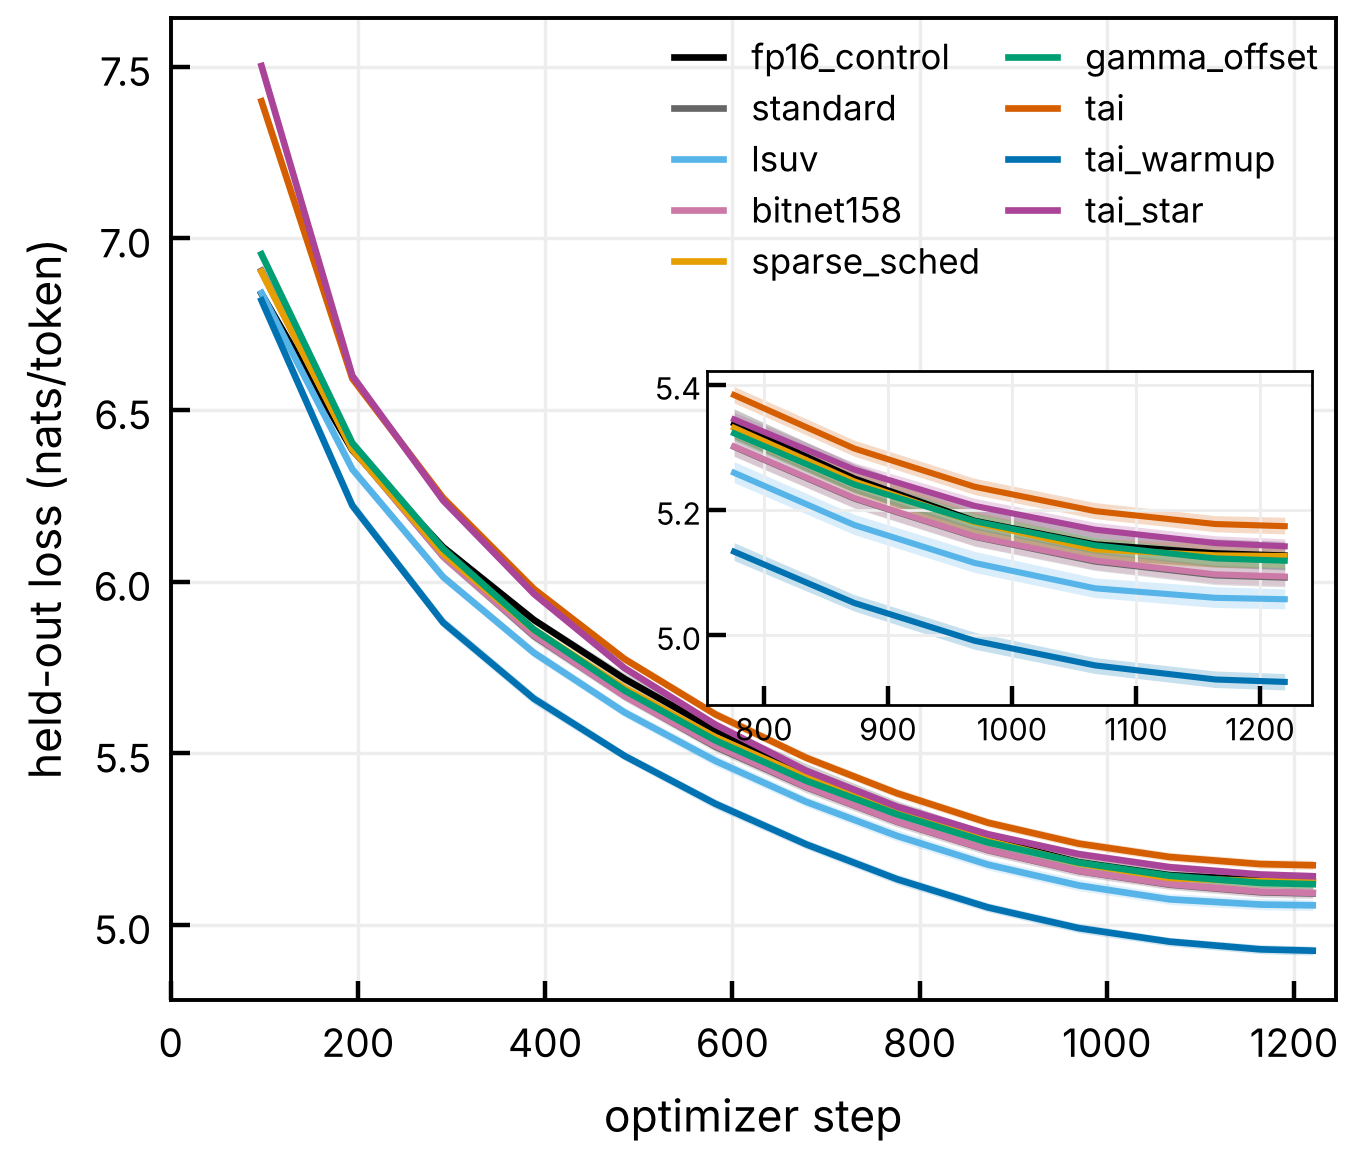
\includegraphics[width=0.86\linewidth]{fig1_convergence.png}
\caption{Held-out loss against optimization step for each arm at the primary
confirmatory scale (\texttt{dim384}), averaged over $15$ seeds at a matched
$20$\,M-token budget. Shaded bands are bootstrap 95\% confidence intervals.}
\label{fig:convergence}
\end{figure}

Table~\ref{tab:primary} reports the complete arm set at the primary
confirmatory scale. Figure~\ref{fig:convergence} shows the corresponding loss
trajectories and Fig.~\ref{fig:finalloss} the paired contrast against the
pre-registered baseline at every ladder point.

\begin{table}[t]
\centering
\footnotesize
\caption{Complete method set at the primary confirmatory scale
(\texttt{dim384}, $8.26$\,M non-embedding parameters, $n=15$ seeds,
$20$\,M-token budget). $\mathcal{L}$: held-out cross-entropy (nats/token);
CI: half-width of the 95\% confidence interval of the mean
(Student $t$, $n=15$); $s$: standard
deviation across seeds; $\mathrm{sp}_T$: final ternary sparsity;
$S_{\mathrm{target}}$: steps to reach the calibrated target loss of $5.6539$
nats; $a_{\mathrm{nt}}$: next-token top-1 accuracy. The pre-registered primary
baseline is \texttt{bitnet158}.}
\label{tab:primary}
\begin{tabular}{@{}lrrrrrr@{}}
\toprule
Arm & $\mathcal{L}$ & CI & $s$ & $\mathrm{sp}_T$ & $S_{\mathrm{target}}$ & $a_{\mathrm{nt}}$ \\
\midrule
\texttt{fp16\_control} & 5.1785 & 0.0248 & 0.0447 & \phantom{0}0.0\% & 564 & 0.216 \\
\texttt{standard} & 5.1094 & 0.0170 & 0.0307 & 32.1\% & 552 & 0.227 \\
\texttt{lsuv} & 5.0752 & 0.0185 & 0.0334 & 31.8\% & 524 & 0.230 \\
\texttt{bitnet158} & 5.1114 & 0.0161 & 0.0291 & 32.1\% & 555 & 0.227 \\
\texttt{sparse\_sched} & 5.1440 & 0.0205 & 0.0370 & 48.8\% & 564 & 0.224 \\
\texttt{gamma\_offset} & 5.1365 & 0.0143 & 0.0258 & 26.0\% & 560 & 0.224 \\
\texttt{tai} & 5.1914 & 0.0150 & 0.0271 & 30.0\% & 613 & 0.221 \\
\textbf{\texttt{tai\_warmup}} & \textbf{4.9437} & 0.0150 & 0.0272 & 30.3\% & \textbf{448} & \textbf{0.242} \\
\texttt{tai\_star} & 5.1919 & 0.0135 & 0.0244 & 28.4\% & 589 & 0.218 \\
\bottomrule
\end{tabular}
\end{table}

Three orderings organize the results. The first two are reproduced at every
ladder point (Fig.~\ref{fig:finalloss}).

\begin{enumerate}
\renewcommand{\labelenumi}{(\roman{enumi})}
\item \textbf{\texttt{tai\_warmup} attains the lowest loss of any arm.} At the
primary scale it improves on the pre-registered baseline by $0.168$ nats and
on the full-precision control by $0.235$ nats.

\item \textbf{\texttt{tai} attains a higher loss than every locked-$\rhoz$
ternary baseline.} At the primary scale it is $0.080$ nats above
\texttt{bitnet158} and $0.116$ nats above \texttt{lsuv}. The two variants of
the proposed method therefore lie on opposite sides of the baseline, and
\texttt{tai\_star} (Section~\ref{sec:res-h8}) tracks \texttt{tai}.

\item \textbf{The gradual-pruning baseline \texttt{sparse\_sched} is the
weakest ternary baseline at the primary scale} ($5.1440$ nats) while attaining by far the highest sparsity
($48.8\%$), and \texttt{gamma\_offset} at its grid-default $\rhoz = 0.75$ sits
between the locked baselines and \texttt{tai}.
\end{enumerate}

\begin{figure*}[t]
\centering
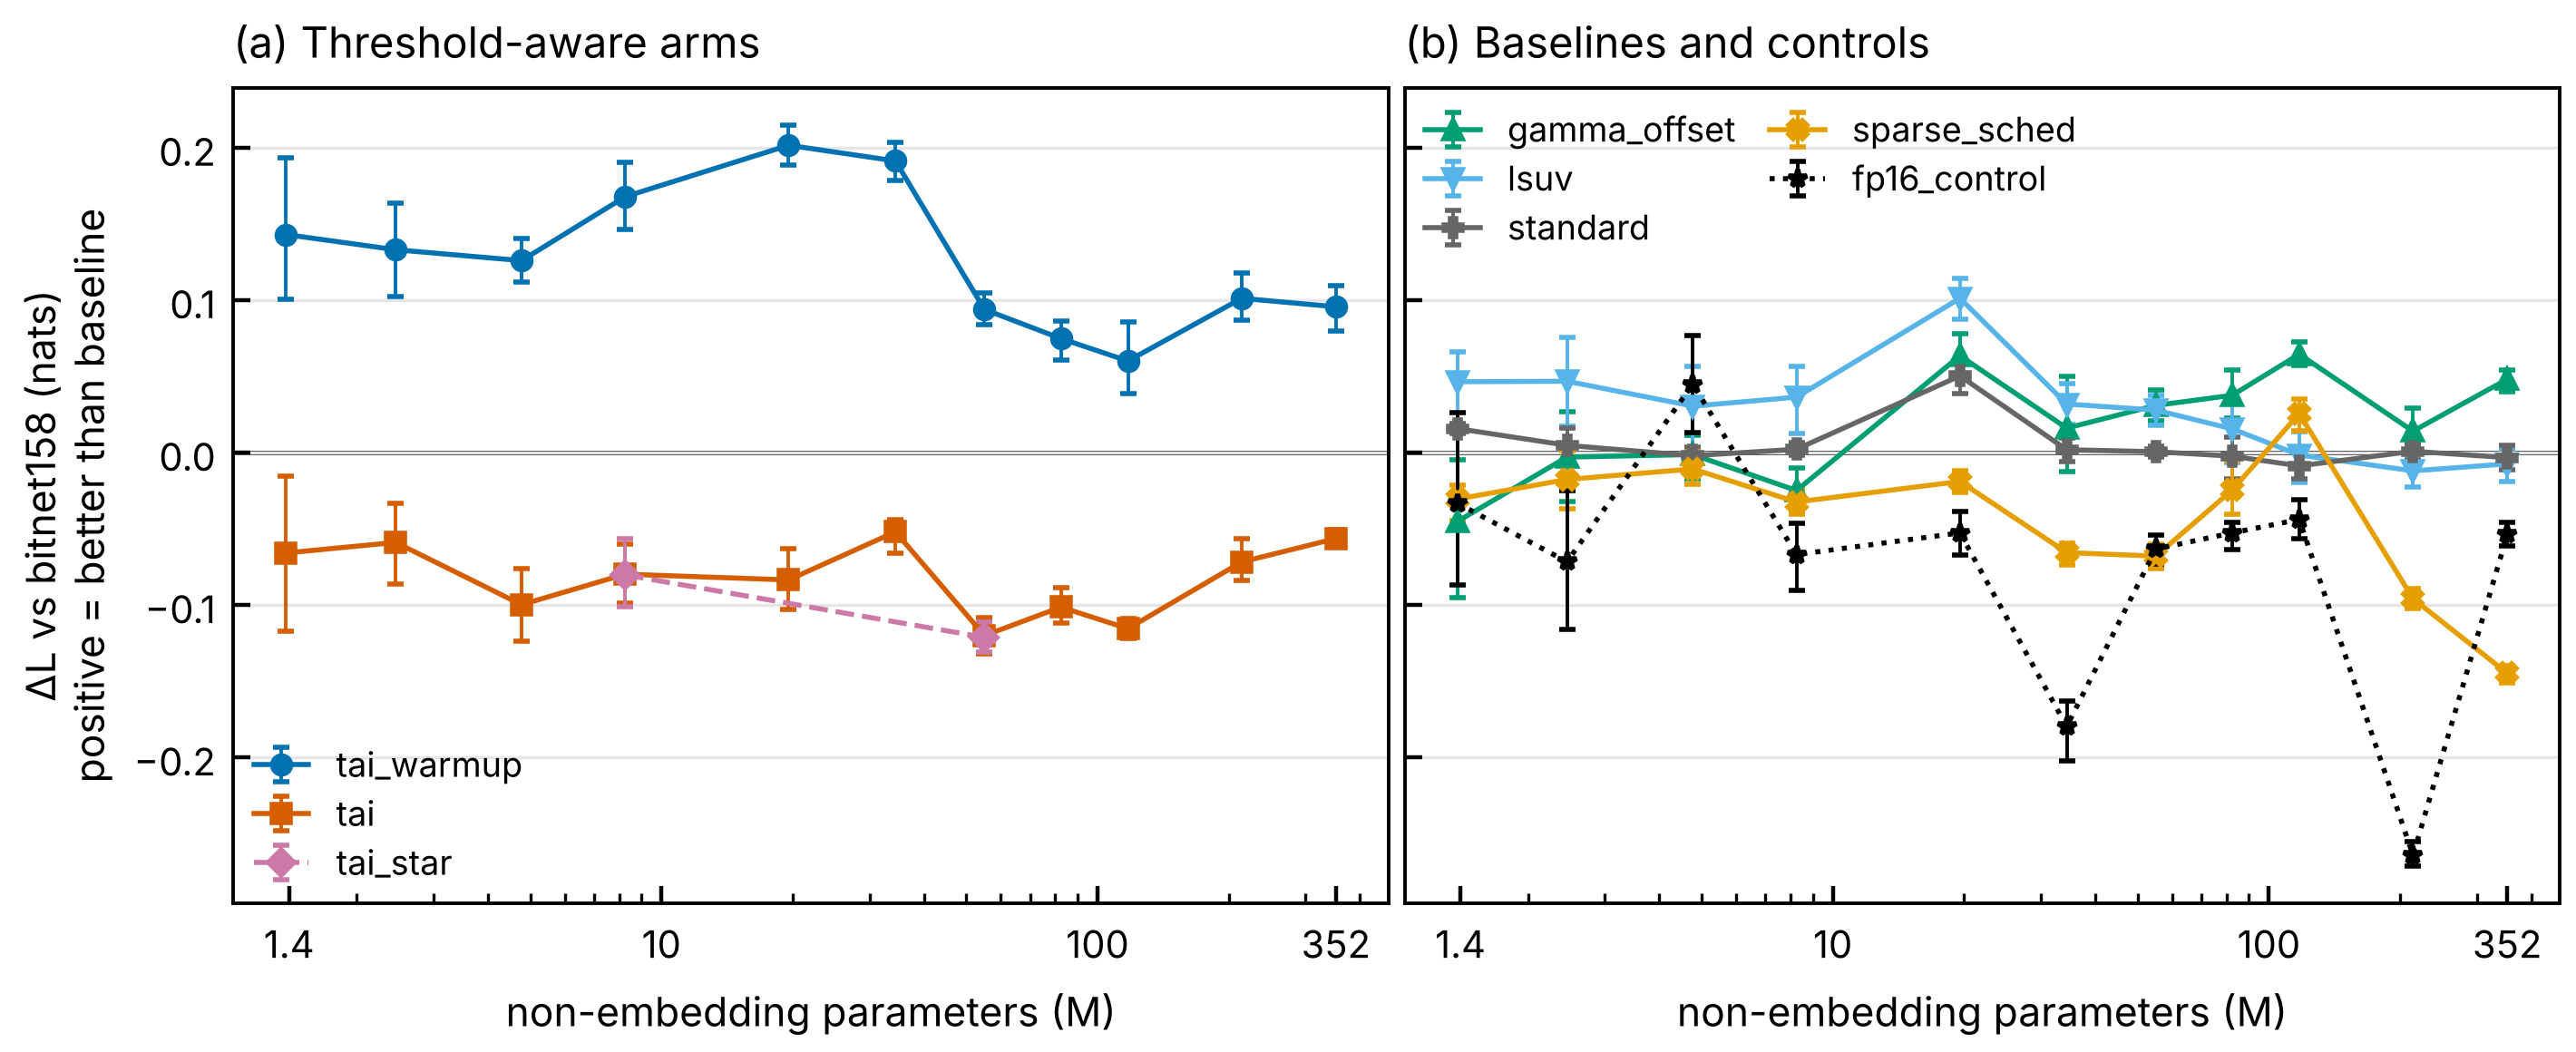
\includegraphics[width=\linewidth]{fig2_final_loss.png}
\caption{Paired quality contrast against the pre-registered baseline across the
eleven-point ladder. Each point is
$\dL = \mathcal{L}(\texttt{bitnet158}) - \mathcal{L}(\mathrm{arm})$, averaged
over the seeds the two arms share at that scale, so positive values favour the
arm; bars are bootstrap 95\% confidence intervals over seeds ($n = 15$ at the
four confirmatory scales, $n = 5$ elsewhere). Panel (a): the threshold-aware
arms, with \texttt{tai\_warmup} above the baseline at every scale and
\texttt{tai} below it at every scale. Panel (b): the remaining baselines and
the full-precision control. \texttt{tai\_star} was executed at \texttt{dim384}
and \texttt{dim768} only. Absolute losses at the primary scale are in
Table~\ref{tab:primary}; the differences are plotted here because they span
$0.26$ nats against absolute losses near $5$.}
\label{fig:finalloss}
\end{figure*}

A result that requires explicit statement is that the ternary arms do not sit
above the full-precision control at this budget. That control is named
\texttt{fp16\_control} after its harness identifier but runs in
\texttt{bfloat16} throughout (Table~\ref{tab:arms}). Taking the strongest non-TAI
ternary arm at each scale, we find that ternary training attains the lower
loss at ten of the eleven ladder points, by between
$0.080$ and $0.278$ nats; the sole exception is \texttt{dim320}, where
\texttt{bitnet158} is $0.045$ nats above \texttt{fp16\_control}. Two properties
of the protocol are recorded alongside this observation without further
interpretation, which is deferred to Section~\ref{sec:discussion}: the
budget does not reach convergence for any arm (Section~\ref{sec:res-budget}),
and the full-precision arm selects a strictly smaller calibrated learning rate
than the ternary arms at five of the eleven scales, though its optimum is
bracketed by the grid at all of them (Section~\ref{sec:res-validity}).

%-----------------------------------------------------------------------------
\subsection{H1: convergence speed at a matched target loss}
\label{sec:res-h1}

Steps-to-target is measured against the calibrated target of $5.6539$ nats,
fixed before the grid on the disjoint calibration seeds. The results are
reported in the $\dS$ column of Table~\ref{tab:crossscale}.

\texttt{tai\_warmup} reaches the target in fewer steps than the primary
baseline at all eleven scales, with $\dS$ ranging from $+28$ steps
(\texttt{dim1280}) to $+148$ steps (\texttt{dim512}). Every statistic in this
subsection is computed on $S_{\mathrm{target}}$ and is therefore distinct from
the held-out-loss columns of Table~\ref{tab:crossscale}: Cohen's $d$ on steps
lies between $+2.39$ and $+7.95$, all eleven paired $t$-tests reject at
$\alpha = 0.05$, and ten of eleven reject at the standalone level
$\alpha_{0} = 0.0125$ fixed in the design, the exception being
\texttt{dim192} ($p = 0.0138$).

\texttt{tai} requires more steps than the baseline at all eleven scales,
with $\dS$ between $-48$ and $-100$ and steps-based $d$ between $-1.52$ and
$-4.47$; ten of eleven contrasts are significant at $\alpha = 0.05$ (\texttt{dim192}:
$p = 0.1248$).

H1 as pre-registered is therefore supported for the schedule variant and
rejected in the opposite direction for the fixed-$\rhoz$ variant.

%-----------------------------------------------------------------------------
\subsection{H2: quality at a fixed token budget}
\label{sec:res-h2}

The pre-registered convergence-conditional test is untestable
(Section~\ref{sec:res-budget}). The token-equal companion test, defined over
all paired seeds against the data-derived margin
$\Delta_{\mathrm{eq}} = 0.10\,|\bar{\mathcal{L}}^{(\beta)} -
\bar{\mathcal{L}}^{(\mathrm{fp16})}|$, is reported in
Table~\ref{tab:crossscale}.

\begin{table*}[t]
\centering
\scriptsize
\caption{Cross-scale paired contrasts against the pre-registered primary
baseline \texttt{bitnet158}. $\dL$ and $\dS$ follow Eq.~\eqref{eq:dL}
(positive favours the method). $\mathrm{CI}_{95}$ is the nonparametric
bootstrap interval on $\dL$ over $5{,}000$ resamples; $d$ is Cohen's $d$;
$p_t$ is the paired $t$-test $p$-value; $p_{\mathrm{Lev}}$ is Levene's test for
H4; $\Delta_{\mathrm{eq}}$ is the data-derived equivalence margin, one value
per scale. The verdict column is the token-equal companion decision. Confirmatory scales are set in
bold. $n$ is the number of paired seeds.}
\label{tab:crossscale}
\begin{tabular}{@{}llrrrrrrrrl@{}}
\toprule
Scale & Arm & $n$ & $\dL$ & $\mathrm{CI}_{95}$ & $d$ & $p_t$ & $\dS$ & $p_{\mathrm{Lev}}$ & $\Delta_{\mathrm{eq}}$ & Verdict \\
\midrule
\texttt{dim192} & \texttt{tai} & 5 & $-0.0661$ & $[-0.117,-0.016]$ & $-1.83$ & 0.0922 & $-88$ & 0.615 & 0.0033 & inconclusive \\
& \texttt{tai\_warmup} & 5 & $+0.1428$ & $[+0.101,+0.191]$ & $+4.33$ & 0.0051 & $+108$ & 0.285 &  & better \\
\textbf{\texttt{dim256}} & \texttt{tai} & 15 & $-0.0591$ & $[-0.086,-0.033]$ & $-1.45$ & 0.0008 & $-63$ & 0.036 & 0.0072 & worse \\
& \texttt{tai\_warmup} & 15 & $+0.1329$ & $[+0.102,+0.164]$ & $+2.88$ & $<10^{-4}$ & $+101$ & 0.447 &  & better \\
\texttt{dim320} & \texttt{tai} & 5 & $-0.1000$ & $[-0.124,-0.076]$ & $-4.79$ & 0.0021 & $-100$ & 0.996 & 0.0045 & worse \\
& \texttt{tai\_warmup} & 5 & $+0.1257$ & $[+0.111,+0.140]$ & $+5.31$ & 0.0001 & $+92$ & 0.707 &  & better \\
\textbf{\texttt{dim384}} & \texttt{tai} & 15 & $-0.0800$ & $[-0.099,-0.060]$ & $-2.84$ & $<10^{-4}$ & $-59$ & 0.648 & 0.0067 & worse \\
& \texttt{tai\_warmup} & 15 & $+0.1677$ & $[+0.146,+0.190]$ & $+5.95$ & $<10^{-4}$ & $+107$ & 0.889 &  & better \\
& \texttt{tai\_star} & 15 & $-0.0805$ & $[-0.102,-0.057]$ & $-3.00$ & $<10^{-4}$ & $-35$ & 0.532 &  & worse \\
\textbf{\texttt{dim512}} & \texttt{tai} & 15 & $-0.0838$ & $[-0.104,-0.064]$ & $-3.59$ & $<10^{-4}$ & $-71$ & 0.175 & 0.0053 & worse \\
& \texttt{tai\_warmup} & 15 & $+0.2014$ & $[+0.188,+0.214]$ & $+11.26$ & $<10^{-4}$ & $+148$ & 0.347 &  & better \\
\texttt{dim640} & \texttt{tai} & 5 & $-0.0522$ & $[-0.066,-0.044]$ & $-5.12$ & 0.0016 & $-48$ & 0.871 & 0.0180 & worse \\
& \texttt{tai\_warmup} & 5 & $+0.1911$ & $[+0.178,+0.204]$ & $+13.01$ & $<10^{-4}$ & $+104$ & 0.633 &  & better \\
\textbf{\texttt{dim768}} & \texttt{tai} & 15 & $-0.1203$ & $[-0.132,-0.109]$ & $-6.35$ & $<10^{-4}$ & $-95$ & 0.957 & 0.0063 & worse \\
& \texttt{tai\_warmup} & 15 & $+0.0937$ & $[+0.084,+0.105]$ & $+5.32$ & $<10^{-4}$ & $+53$ & 0.593 &  & better \\
& \texttt{tai\_star} & 15 & $-0.1214$ & $[-0.131,-0.111]$ & $-7.23$ & $<10^{-4}$ & $-95$ & 0.461 &  & worse \\
\texttt{dim896} & \texttt{tai} & 5 & $-0.1016$ & $[-0.112,-0.091]$ & $-6.63$ & 0.0001 & $-72$ & 0.360 & 0.0053 & worse \\
& \texttt{tai\_warmup} & 5 & $+0.0746$ & $[+0.061,+0.086]$ & $+6.38$ & 0.0006 & $+40$ & 0.819 &  & better \\
\texttt{dim1024} & \texttt{tai} & 5 & $-0.1157$ & $[-0.122,-0.109]$ & $-12.12$ & $<10^{-4}$ & $-100$ & 0.334 & 0.0044 & worse \\
& \texttt{tai\_warmup} & 5 & $+0.0599$ & $[+0.039,+0.085]$ & $+3.48$ & 0.0102 & $+32$ & 0.621 &  & better \\
\texttt{dim1280} & \texttt{tai} & 5 & $-0.0720$ & $[-0.084,-0.057]$ & $-5.75$ & 0.0008 & $-72$ & 0.389 & 0.0264 & worse \\
& \texttt{tai\_warmup} & 5 & $+0.1010$ & $[+0.087,+0.116]$ & $+8.99$ & 0.0003 & $+28$ & 0.163 &  & better \\
\texttt{dim1536} & \texttt{tai} & 5 & $-0.0566$ & $[-0.062,-0.051]$ & $-5.81$ & 0.0001 & $-68$ & 0.385 & 0.0054 & worse \\
& \texttt{tai\_warmup} & 5 & $+0.0954$ & $[+0.079,+0.110]$ & $+8.27$ & 0.0004 & $+36$ & 0.955 &  & better \\
\bottomrule
\end{tabular}
\end{table*}

The bootstrap interval excludes zero in all $24$ cells, so the sign of $\dL$
is resolved throughout. The one cell whose paired $t$-test does not reach
$\alpha = 0.05$ is \texttt{tai} at \texttt{dim192} ($n=5$, $p_t = 0.0922$),
which is why its verdict is inconclusive. The companion test never returns equivalence: $\Delta_{\mathrm{eq}}$
ranges from $0.0033$ to $0.0264$ nats while $|\dL|$ ranges from $0.052$ to
$0.201$ nats, i.e.\ every observed difference exceeds its margin by between
$2.7\times$ and $42.9\times$. The verdicts are accordingly categorical:
\texttt{tai\_warmup} is superior to the baseline at all eleven scales;
\texttt{tai} is inferior at ten of eleven and inconclusive at the eleventh.

Holm--Bonferroni correction within the confirmatory held-out-loss family, at
family-wise level $\alpha_{H} = 0.05$, rejects the null for both TAI variants
at every scale except \texttt{tai} at \texttt{dim192}, which is retained. The Wilcoxon signed-rank test, computed
wherever $n \geq 6$, supports the parametric verdict in every case
($p \leq 0.0009$).

The secondary sensitivity contrast against the data-selected minimum baseline
attenuates the \texttt{tai\_warmup} advantage, for
example at \texttt{dim512}, $\dL$ falls from $+0.201$ (versus
\texttt{bitnet158}) to $+0.100$ (versus \texttt{lsuv}), and at \texttt{dim768}
from $+0.094$ to $+0.063$ (versus \texttt{gamma\_offset}). The sign survives at
ten of the eleven scales and reverses at \texttt{dim1024}, where
\texttt{gamma\_offset} is the strongest baseline and $\dL = -0.0044$. This contrast is
exploratory and carries no family-wise correction.

%-----------------------------------------------------------------------------
\subsection{H4: outcome variance}
\label{sec:res-h4}

Levene's test finds no evidence that either TAI variant inflates variance
relative to the baseline. Across the $24$ cells of Table~\ref{tab:crossscale},
$p_{\mathrm{Lev}}$ falls below $0.05$ in exactly one
(\texttt{dim256}/\texttt{tai}, $p = 0.036$). That cell does not bear on H4 in
the direction the hypothesis concerns: the TAI standard deviation there is
less than half the baseline's ($0.0237$ versus $0.0525$), so what the test
detects is a reduction in spread, not inflation. It also does not survive the
pre-registered per-hypothesis level $\alpha_{0} = 0.0125$.

The pre-registered form of H4 is evaluated on the pooled seed $\times$ fold
matrix, in which every trained model is scored on all $K=5$ held-out sub-folds.
Table~\ref{tab:h4} reports the decomposition at the primary scale.

\begin{table}[t]
\centering
\small
\caption{Variance decomposition for H4 at the primary scale
(\texttt{dim384}, $15$ seeds $\times$ $5$ held-out folds). Mean $\mathcal{L}$
is the grand mean over all five folds and therefore differs from the fold-$0$
value of Table~\ref{tab:primary}. Levene's test on the
pooled matrix is the pre-registered statistic.}
\label{tab:h4}
\begin{tabular}{@{}lrrrr@{}}
\toprule
Arm & Mean $\mathcal{L}$ & $s$ across seeds & $s$ across folds & $s$ pooled \\
\midrule
\texttt{tai} & 5.2113 & 0.0272 & 0.0328 & 0.0397 \\
\texttt{bitnet158} & 5.1324 & 0.0309 & 0.0339 & 0.0429 \\
\midrule
\multicolumn{5}{@{}l}{Levene, pooled seed $\times$ fold: $W = 0.554$, $p = 0.458$} \\
\multicolumn{5}{@{}l}{Levene, seed only: $W = 0.343$, $p = 0.563$} \\
\bottomrule
\end{tabular}
\end{table}

H4 is supported: there is no evidence of variance inflation
($p = 0.458$, clearing both the conventional $0.05$ and the pre-registered
$\alpha_{0} = 0.0125$), and this holds whether or not data-sampling
spread is included. A secondary observation from the decomposition is that the
dominant variance component is the evaluation fold rather than the seed
(mean $s$ across folds $0.0334$ versus across seeds $0.0290$), for both arms.

%-----------------------------------------------------------------------------
\subsection{H3: control of the ternary operating point and its retention}
\label{sec:res-h3}

\begin{figure}[t]
\centering
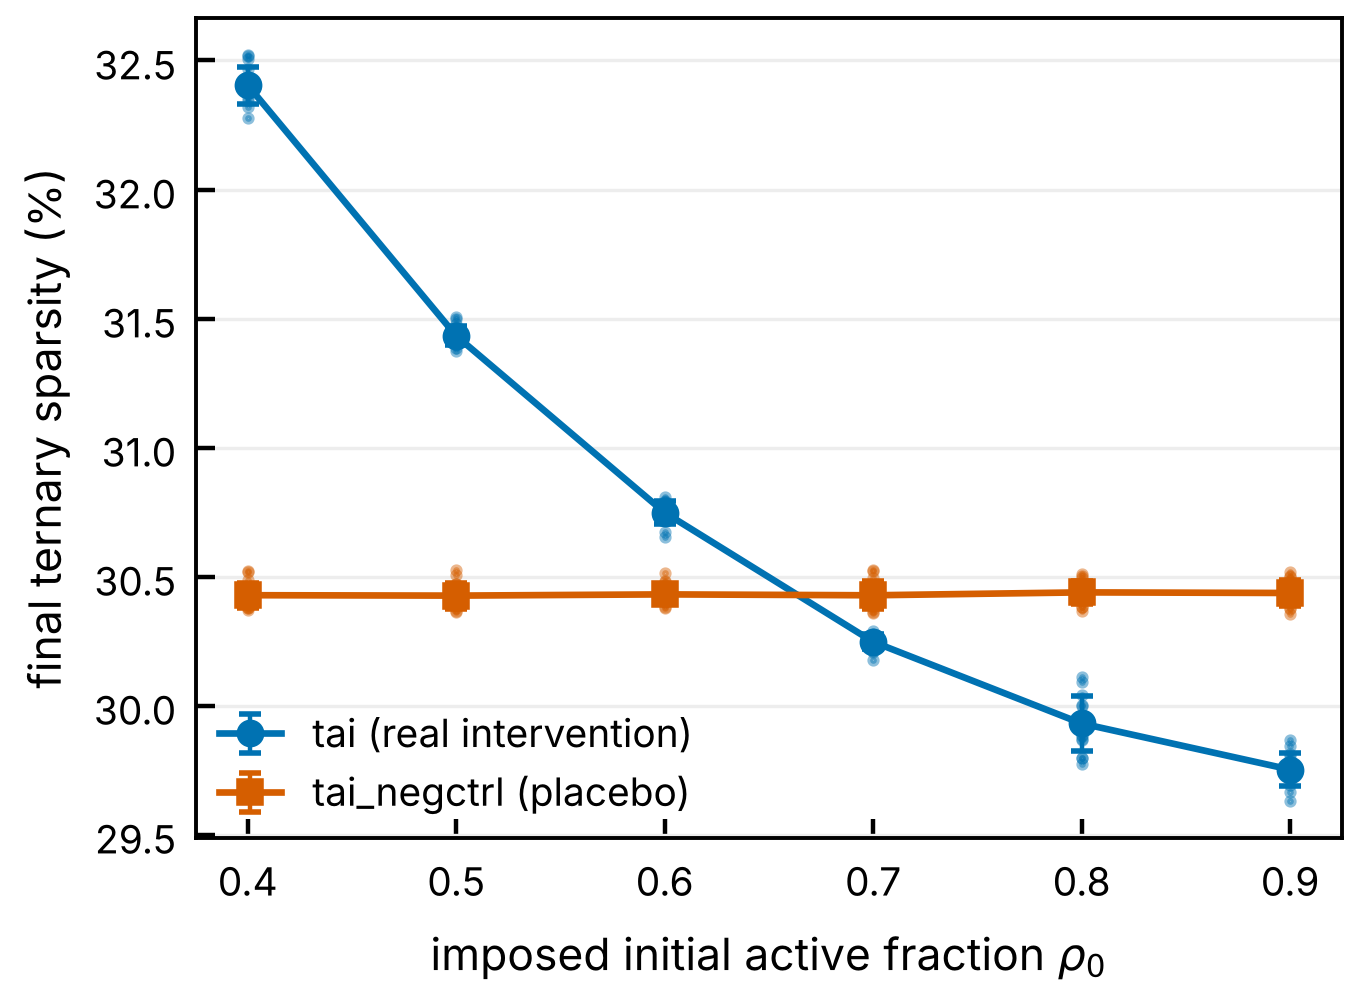
\includegraphics[width=0.86\linewidth]{fig3_rho0_sweep.png}
\caption{Final ternary sparsity, in per cent, as a function of the imposed
initial active fraction $\rhoz$ at the primary scale (\texttt{dim384}), for
the \texttt{tai} arm and for the $\rhoz$-labelled placebo
\texttt{tai\_negctrl}. Every one of the $15$ seeds per point is shown, with
the mean and one standard deviation. The placebo
holds the realized threshold partition fixed at $\rhoz = 0.69$ while varying
only the label, so any dependence it exhibits is measurement artefact.}
\label{fig:sweep}
\end{figure}

\subsubsection{Ordinal control}

The rank association between $\rhoz$ and final sparsity is essentially perfect
and negative, as predicted (Fig.~\ref{fig:sweep}): a larger initial active
fraction implies fewer terminal zeros. At the primary scale the pooled Spearman coefficient is
$-0.983$ ($p = 4.3\times 10^{-66}$) and the mean per-seed coefficient is
$-0.996$, 95\% CI $[-1.000, -0.989]$ over $15$ seeds, with $93\%$ of seeds
strictly monotone. The intervention is far above the nuisance floor: the
across-$\rhoz$ range of final sparsity is $0.0265$ against a within-$\rhoz$
across-seed standard deviation of $0.00059$, a signal-to-noise ratio of
$44.9\times$. The control is statistically indistinguishable across scale
(\texttt{dim384} mean $-0.996 \pm 0.015$ versus \texttt{dim768}
$-1.000 \pm 0.000$; Welch $t = +1.00$, $p = 0.334$).

\subsubsection{Retention: how much of the intervention survives training}

The ordinal result establishes that the ordering survives; it does not
establish that the magnitude does. Regressing final on initial sparsity
per Eq.~\eqref{eq:retention} gives the retention coefficients of
Table~\ref{tab:retention}, which is the principal quantitative result of this
section.

\begin{table*}[t]
\centering
\small
\caption{Retention of the operating-point intervention,
$\mathrm{sp}_T = \mathrm{sp}_\infty + r\,\mathrm{sp}_0$, over the six-point
$\rhoz$ grid at $15$ seeds per point. A $50$-percentage-point swing in initial
sparsity is imposed in every cell. $r$: retention coefficient; final swing: the
resulting range of final sparsity.}
\label{tab:retention}
\begin{tabular}{@{}llrrrr@{}}
\toprule
Scale & Arm & $r$ & $R^{2}$ & Final swing & Implied fixed point \\
\midrule
\texttt{dim384} & \texttt{tai} & 0.052 & 0.931 & \phantom{0}2.65 pt & 0.305 \\
\texttt{dim384} & \texttt{gamma\_offset} & 1.003 & 1.000 & 50.09 pt & n/a \\
\texttt{dim768} & \texttt{tai} & 0.069 & 0.959 & \phantom{0}3.55 pt & 0.300 \\
\texttt{dim768} & \texttt{gamma\_offset} & 1.006 & 1.000 & 50.33 pt & n/a \\
\bottomrule
\end{tabular}
\end{table*}

The two mechanisms behave qualitatively differently. For the TAI arm, a
$50$-point swing in initial sparsity produces a final swing of $2.65$ points at
\texttt{dim384} and $3.55$ points at \texttt{dim768}: retention is
$0.052$--$0.069$, so approximately $93$--$95\%$ of the imposed intervention is
erased during training. The residual is nonetheless perfectly ordered and
highly reproducible, the within-cell standard deviation being $3$--$11\times
10^{-4}$. The implied fixed point is $0.305$ at \texttt{dim384} and $0.300$ at
\texttt{dim768}; for reference, the \texttt{standard} arm reaches $0.321$ and
$0.318$ at those scales without any intervention.

For the $\gamma$-offset arm, retention is $1.003$ and $1.006$ with
$R^{2} = 1.000$ at both scales: the final operating point tracks the target
one-for-one across the entire $50$-point range
(Table~\ref{tab:sweep}). This arm reaches its operating point by holding the
threshold scale at the constant $c^{\star}(\rhoz)$ of Eq.~\eqref{eq:cstar},
whose calibrated values over the grid are $2.110$, $1.691$, $1.314$, $0.966$,
$0.635$ and $0.315$ for $\rhoz = 0.4,\dots,0.9$.

H3 as pre-registered, that the initial operating point causally shapes the
final learned sparsity, is therefore \textbf{not supported in its strong form
for the initialization mechanism}, and is supported almost exactly for the
threshold-offset mechanism. The operative statement for the initialization
variant is a bounded residual effect with the retention fraction reported.

\subsubsection{Pre-registered falsification}

\begin{figure*}[t]
\centering
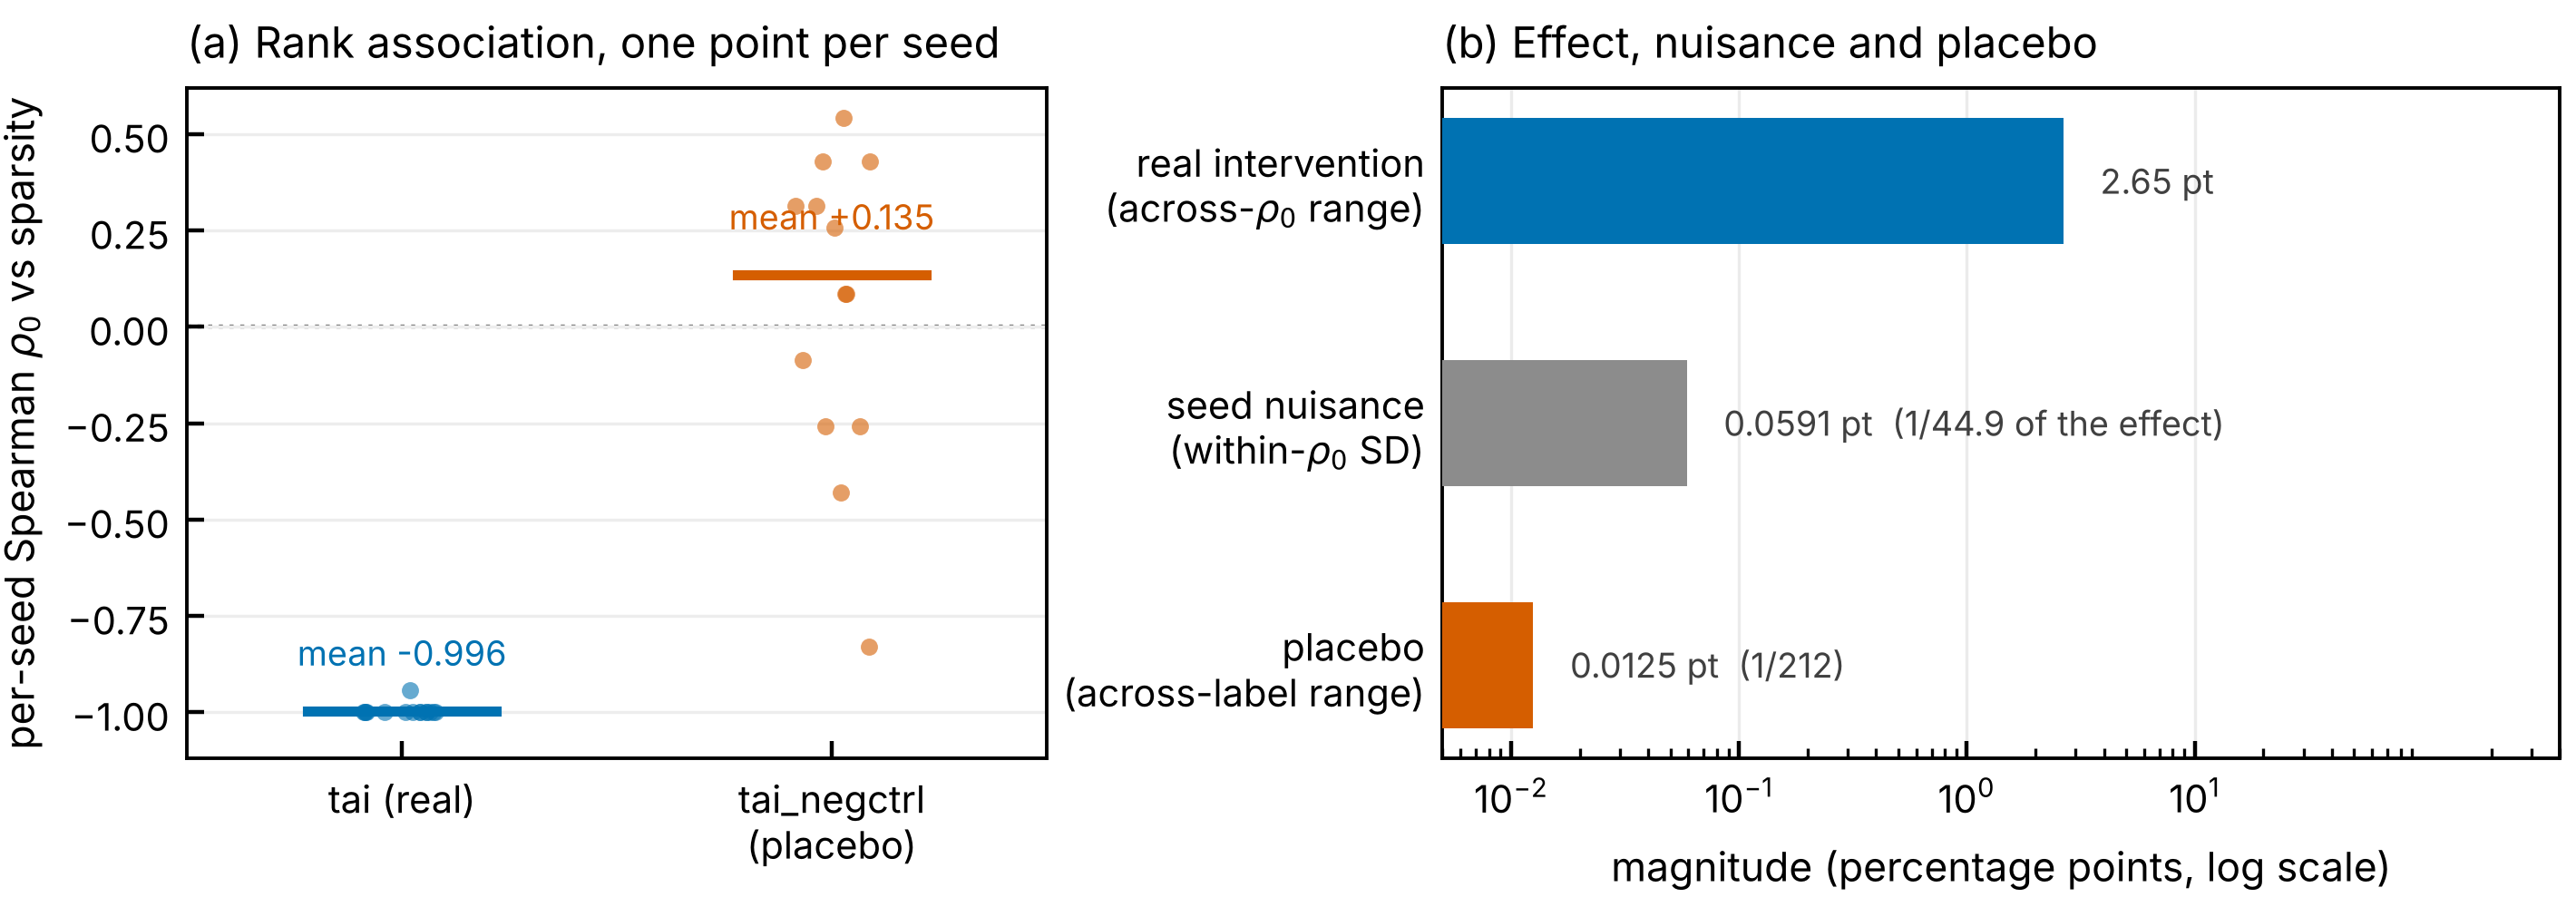
\includegraphics[width=\linewidth]{fig7_h3_falsification.png}
\caption{Pre-registered falsification instrument for H3; the sweep itself is
Fig.~\ref{fig:sweep}. Panel (a): the per-seed Spearman coefficient between the
imposed $\rhoz$ label and final sparsity, one point per seed, for the real
intervention and for the placebo \texttt{tai\_negctrl}. Panel (b): the
across-$\rhoz$ effect, the within-$\rhoz$ seed nuisance and the placebo's
across-label range on one logarithmic axis, so that both ratios quoted in the
text are legible at once. The signed sign test of the pre-registration
($0$ of $15$, $p = 6.1\times10^{-5}$) is not plotted, for the reason given in
the text.}
\label{fig:falsification}
\end{figure*}

The placebo arm \texttt{tai\_negctrl}, which varies the $\rhoz$ label while
holding the realized partition fixed at $0.69$ (Fig.~\ref{fig:falsification}),
produces a final sparsity of $0.3043$--$0.3044$
across all six labels ($n = 15$ per label): a range of
$1.3\times 10^{-4}$, against $2.65\times 10^{-2}$ for the real intervention, a
factor of $212$. The placebo's mean per-seed Spearman coefficient is $+0.135$,
generated entirely by fourth-decimal noise and of opposite sign to the real
effect ($-0.996$). The pre-registered sign test records the real coefficient as
exceeding the placebo coefficient in $0$ of $15$ seeds
($p = 6.1\times 10^{-5}$); because the test was specified as a one-sided
comparison of signed coefficients while the true effect is negative, this
statistic is reported here for completeness and the magnitude comparison above
is the interpretable falsification result. The placebo is flat, as predicted,
and the sparsity effect is therefore not an artefact of the analysis.

%-----------------------------------------------------------------------------
\subsection{H5: the quality-sparsity frontier}
\label{sec:res-h5}

\begin{figure*}[t]
\centering
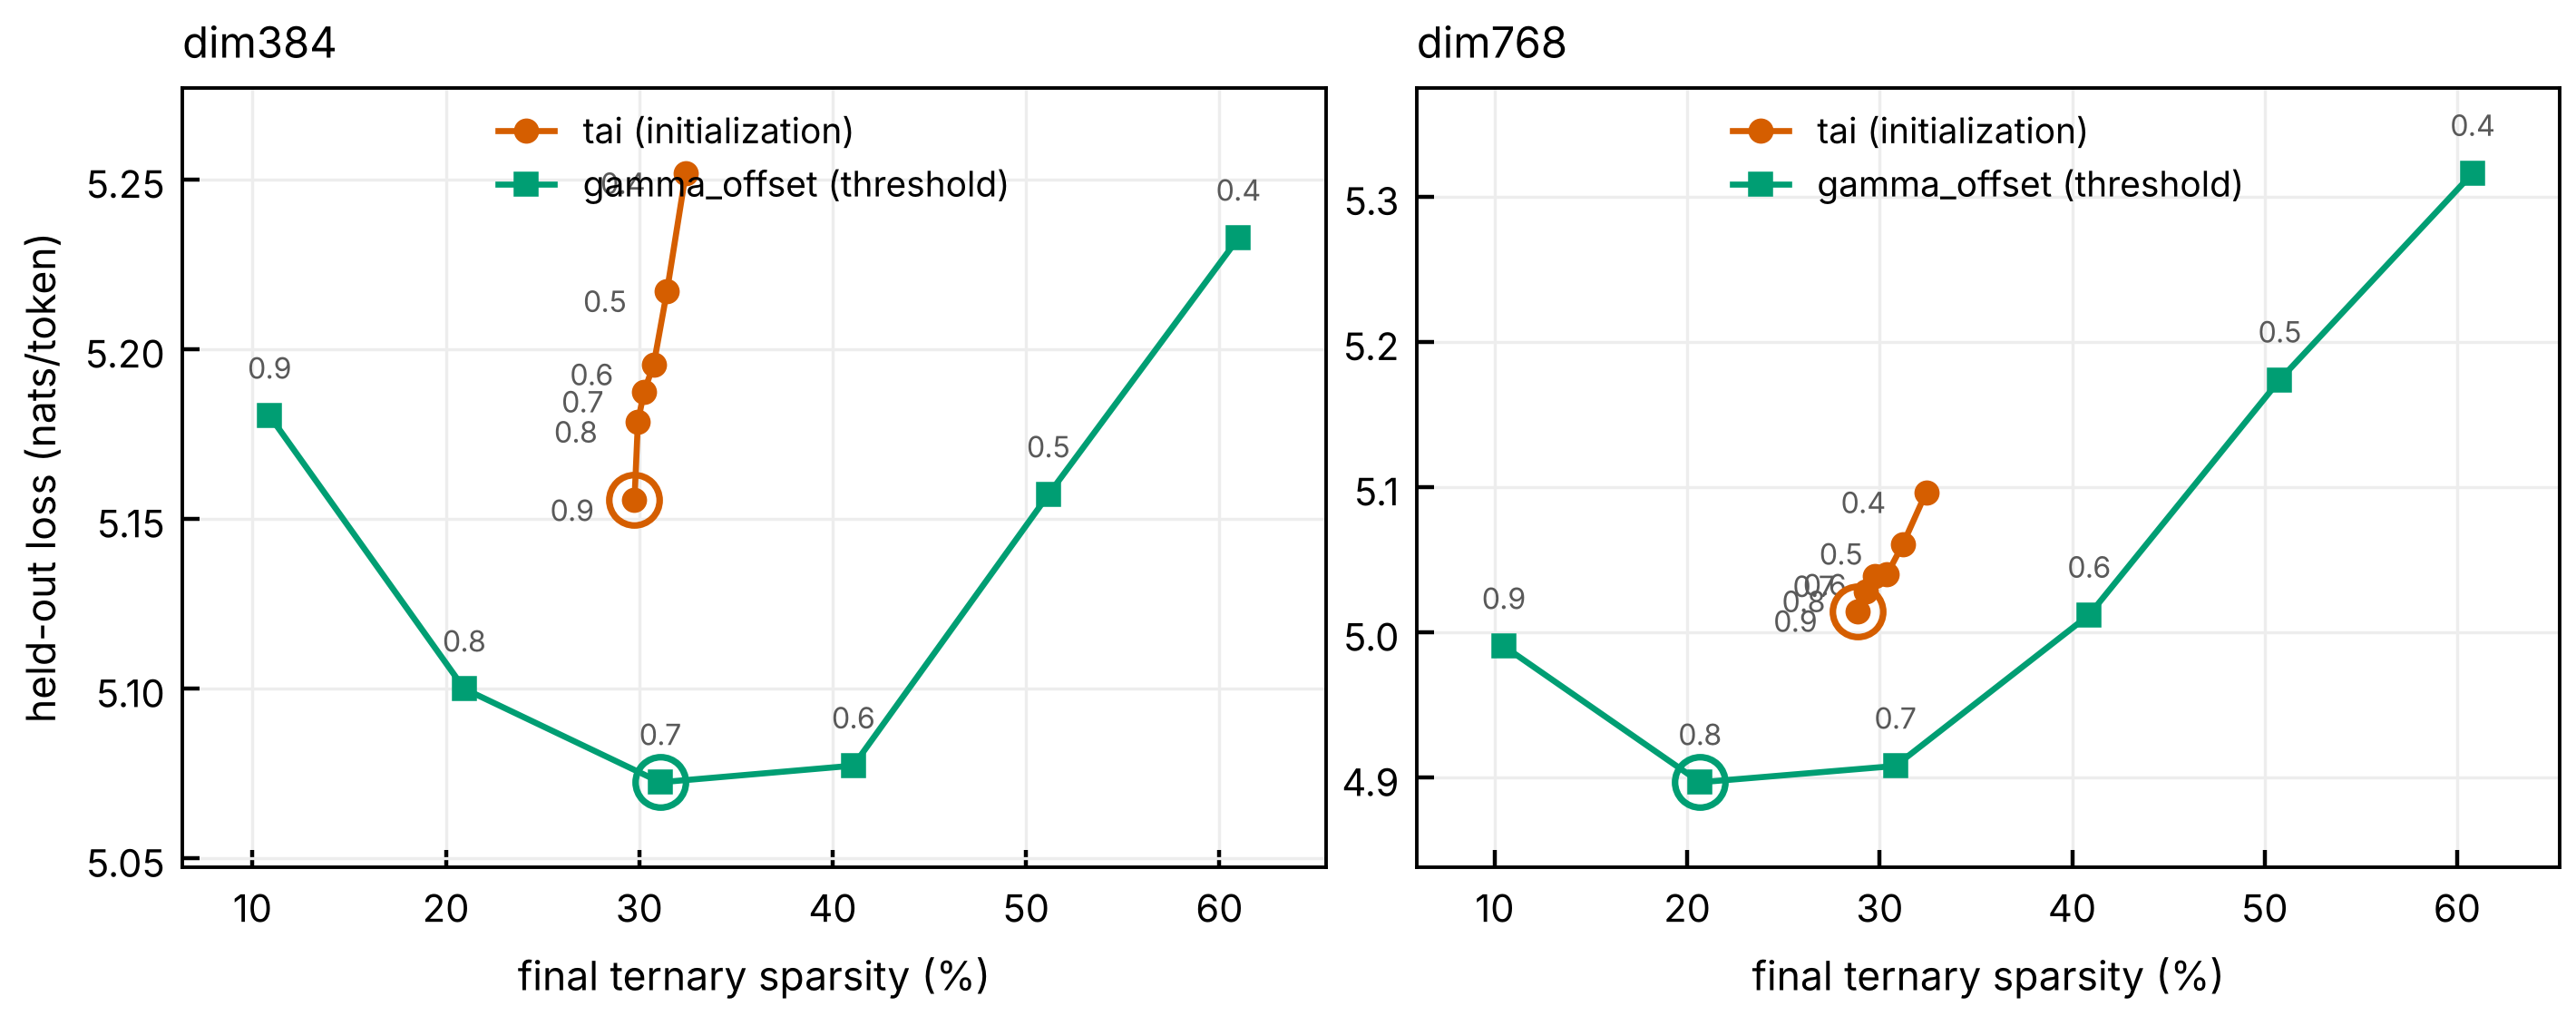
\includegraphics[width=\linewidth]{fig5_pareto.png}
\caption{Held-out loss, in nats per token, against final ternary sparsity, in
per cent, across the $\rhoz$ sweep, for both mechanisms and at both swept
scales. Each point is one operating point, labelled with its $\rhoz$ and
averaged over $15$ seeds; the ringed marker is
each arm's minimum. The threshold-offset arm traces a U-shaped frontier
spanning $50$ points of sparsity with an interior optimum, while the
initialization arm's sparsity axis spans under four points, rendering its
frontier near-degenerate.}
\label{fig:pareto}
\end{figure*}

Table~\ref{tab:sweep} reports the full sweep for both arms at both scales.

\begin{table*}[t]
\centering
\small
\caption{Operating-point sweep. Held-out loss (mean $\pm$ SD over $15$ seeds)
and final ternary sparsity for the initialization mechanism (\texttt{tai}) and
the threshold-offset mechanism (\texttt{gamma\_offset}) at two scales. The
minimum-loss point of each column is set in bold.}
\label{tab:sweep}
\begin{tabular}{@{}crrrrrrrr@{}}
\toprule
& \multicolumn{4}{c}{\texttt{dim384}} & \multicolumn{4}{c}{\texttt{dim768}} \\
\cmidrule(lr){2-5}\cmidrule(lr){6-9}
& \multicolumn{2}{c}{\texttt{tai}} & \multicolumn{2}{c}{\texttt{gamma\_offset}}
& \multicolumn{2}{c}{\texttt{tai}} & \multicolumn{2}{c}{\texttt{gamma\_offset}} \\
$\rhoz$ & $\mathcal{L}$ & $\mathrm{sp}_T$ & $\mathcal{L}$ & $\mathrm{sp}_T$
& $\mathcal{L}$ & $\mathrm{sp}_T$ & $\mathcal{L}$ & $\mathrm{sp}_T$ \\
\midrule
0.4 & 5.2519 & 32.4\% & 5.2328 & 61.0\% & 5.0963 & 32.4\% & 5.3160 & 60.8\% \\
0.5 & 5.2171 & 31.4\% & 5.1572 & 51.2\% & 5.0609 & 31.2\% & 5.1739 & 50.8\% \\
0.6 & 5.1955 & 30.7\% & 5.0774 & 41.1\% & 5.0397 & 30.4\% & 5.0120 & 40.9\% \\
0.7 & 5.1875 & 30.2\% & \textbf{5.0724} & 31.1\% & 5.0386 & 29.8\% & 4.9080 & 30.8\% \\
0.8 & 5.1786 & 29.9\% & 5.1000 & 21.0\% & 5.0282 & 29.3\% & \textbf{4.8968} & 20.7\% \\
0.9 & \textbf{5.1555} & 29.8\% & 5.1804 & 10.9\% & \textbf{5.0146} & 28.9\% & 4.9905 & 10.5\% \\
\bottomrule
\end{tabular}
\end{table*}

For the initialization mechanism the loss decreases monotonically in $\rhoz$
over the whole grid, from $5.2519$ at $\rhoz = 0.4$ to $5.1555$ at
$\rhoz = 0.9$ (\texttt{dim384}), while final sparsity varies by only $2.6$
points; the frontier is consequently near-degenerate, and all six points are
formally non-dominated only because the sparsity differences, though tiny, are
strictly ordered. Under the pre-registered selection rule, minimum loss
subject to $\mathrm{sp}_T \geq 30\%$, the optimum is
$\rhoz^\star = 0.70$ ($\mathcal{L} = 5.1875$, $\mathrm{sp}_T = 30.2\%$), with
bootstrap selection probabilities $P(0.60) = 0.237$, $P(0.70) = 0.758$ and
$\leq 0.003$ elsewhere.

For the threshold-offset mechanism the loss is U-shaped with an interior
optimum, and the sparsity axis spans $50$ points (Fig.~\ref{fig:pareto}). At \texttt{dim384} the
minimum is at $\rhoz = 0.70$ ($\mathcal{L} = 5.0724$ at $31.1\%$ sparsity); at
\texttt{dim768} it is at $\rhoz = 0.80$ ($\mathcal{L} = 4.8968$ at $20.7\%$
sparsity), where the loss is $0.011$ nats below the same arm's $\rhoz = 0.70$
point and $0.020$ nats below the \texttt{dim768} \texttt{bitnet158} baseline
($4.9167$) at two-thirds of its sparsity.

One point associated with this arm does not lie on the curve its neighbours
describe, and is recorded here. The main grid runs \texttt{gamma\_offset} at
the default $\rhoz = 0.75$, which the sweep grid does not contain; at
\texttt{dim384} that point attains $5.1365$, above both $\rhoz = 0.70$
($5.0724$) and $\rhoz = 0.80$ ($5.1000$), by some five standard errors of the
$15$-seed mean. It is not a configuration error: the realized sparsity
interpolates its two neighbours to within $10^{-4}$, and the calibrated
learning rate and the threshold constant $c^{\star}(0.75)$ are the values the
protocol specifies. The sweep and the main grid do, however, fall on opposite
sides of the execution-path split of Section~\ref{sec:res-validity}. We record
the discrepancy rather than resolve it. Contrasts drawn within a single phase
are unaffected, including the main-grid comparison of this arm against the
baseline in Section~\ref{sec:res-gammadefault}; what the discrepancy rules out
is treating the sweep and the main grid as interchangeable measurements of the
same arm.

H5 is therefore supported for the
threshold-offset mechanism, which traces a genuine frontier, and is
uninformative for the initialization mechanism, whose sparsity axis is
effectively fixed.

%-----------------------------------------------------------------------------
\subsection{Mechanism attribution}
\label{sec:res-mechanism}

\begin{figure*}[t]
\centering
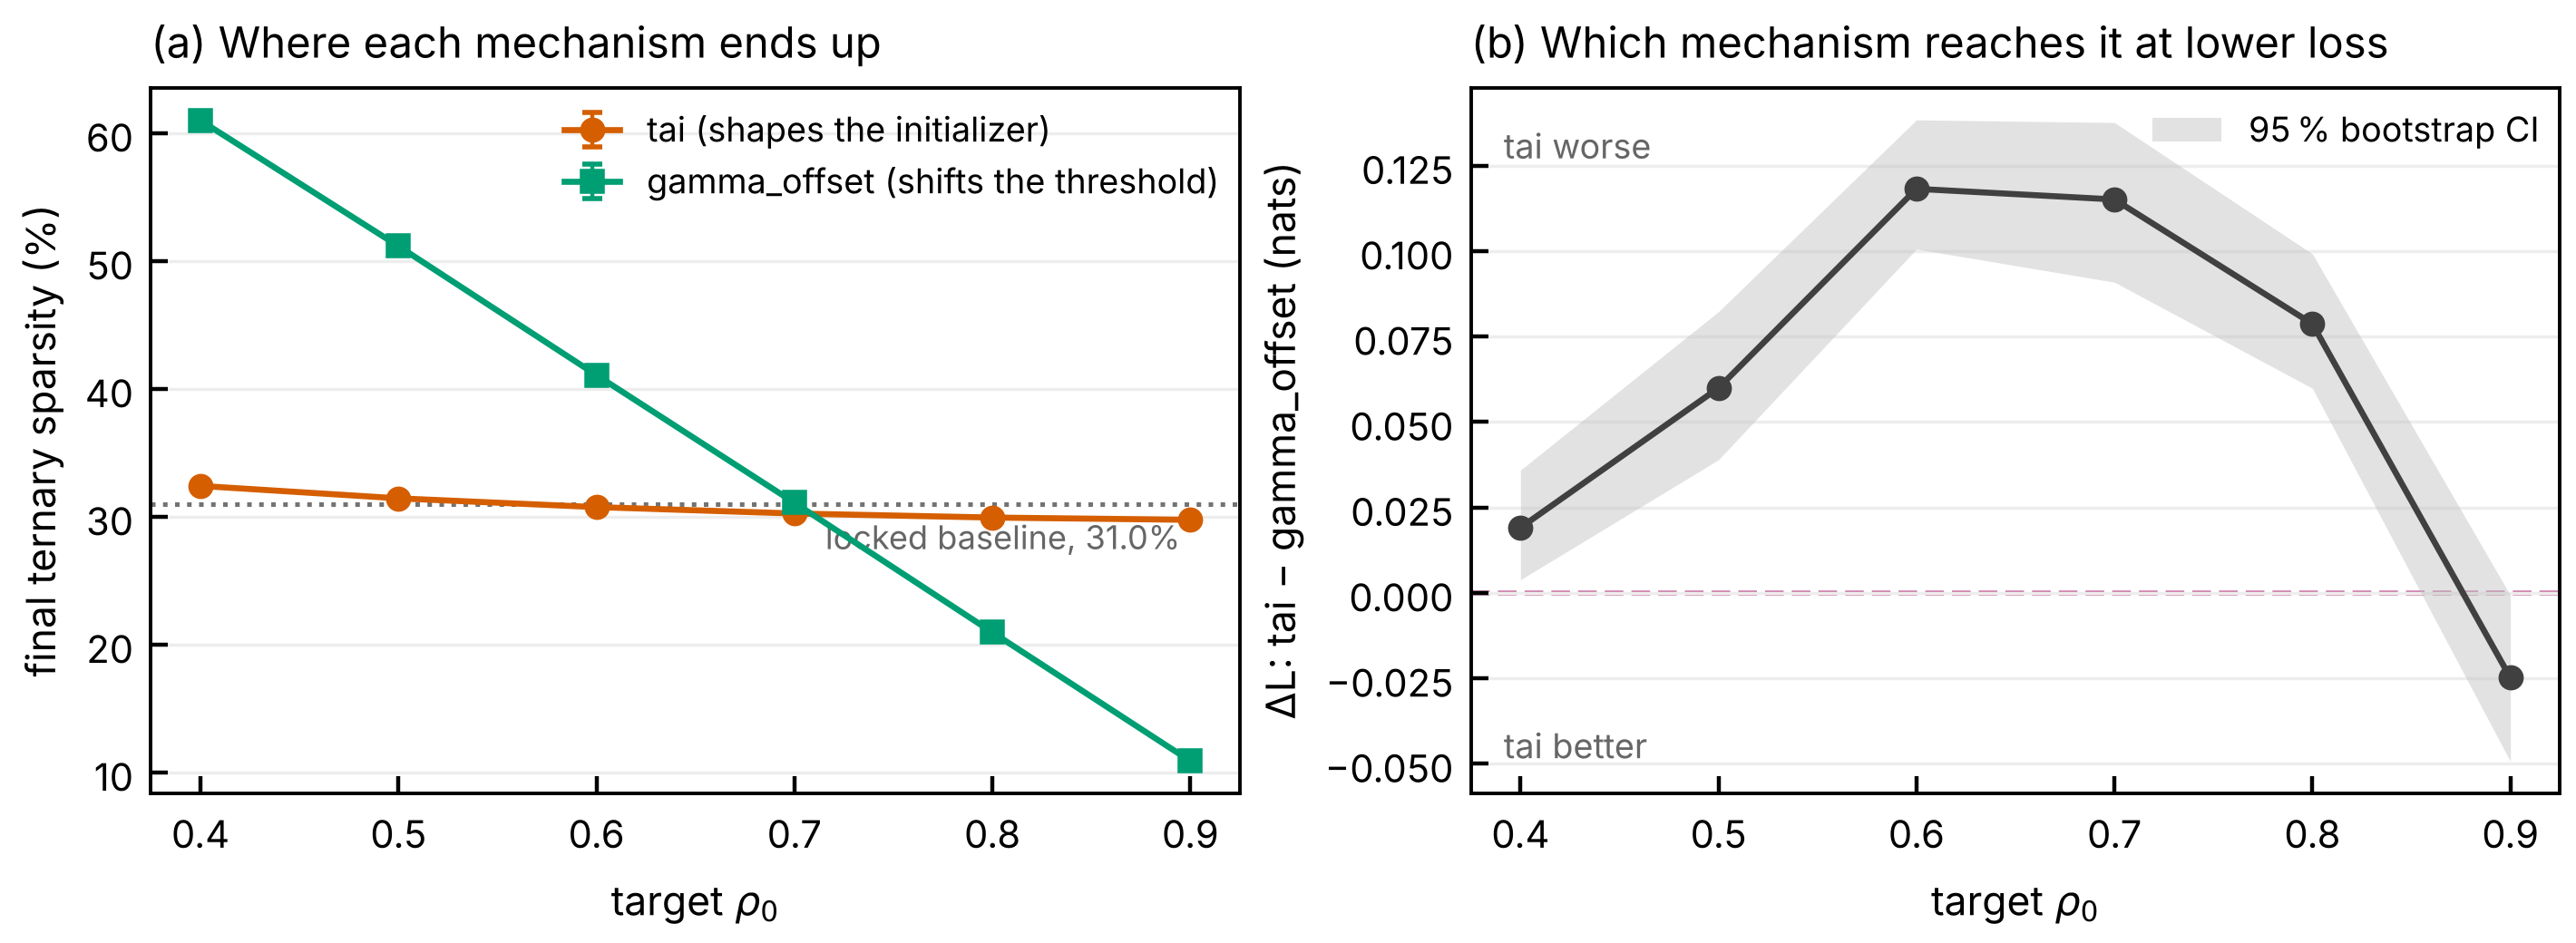
\includegraphics[width=\linewidth]{fig10_mechanism.png}
\caption{Panel (a): the \emph{final} operating point each mechanism reaches as
a function of the target $\rhoz$, with the analytically locked sparsity of
Proposition~\ref{prop:locked} marked. Panel (b): the paired difference in
held-out loss, in nats per token, between the initialization and
threshold-offset mechanisms at matched $\rhoz$, with a bootstrap 95\%
confidence interval over the $15$ seeds; an
interval covering zero would indicate that the two are matched.}
\label{fig:mechanism}
\end{figure*}

\subsubsection{Initialization versus threshold offset}

Paired over all $90$ $(\rhoz, \mathrm{seed})$ cells at the primary scale, the
initialization mechanism attains a loss $0.0610$ nats higher than the
threshold-offset mechanism, 95\% CI $[+0.0474, +0.0742]$, paired
$t$-test $p = 1.06\times 10^{-13}$ (Fig.~\ref{fig:mechanism}). Both arms control the operating point
ordinally with essentially equal reliability (mean per-seed Spearman $-1.000$
for \texttt{gamma\_offset}, $-0.996$ for \texttt{tai}), but only the
threshold-offset arm retains the magnitude (Table~\ref{tab:retention}). Of the
three pre-registered readings of this contrast
(Section~\ref{sec:gammaoffset}), the outcome is the third: the simpler
mechanism wins, on both quality and retention. This contrast is exploratory
and carries no family-wise correction.

\subsubsection{The $2\times 2$ initialization $\times$ precision ablation}

\begin{figure}[t]
\centering
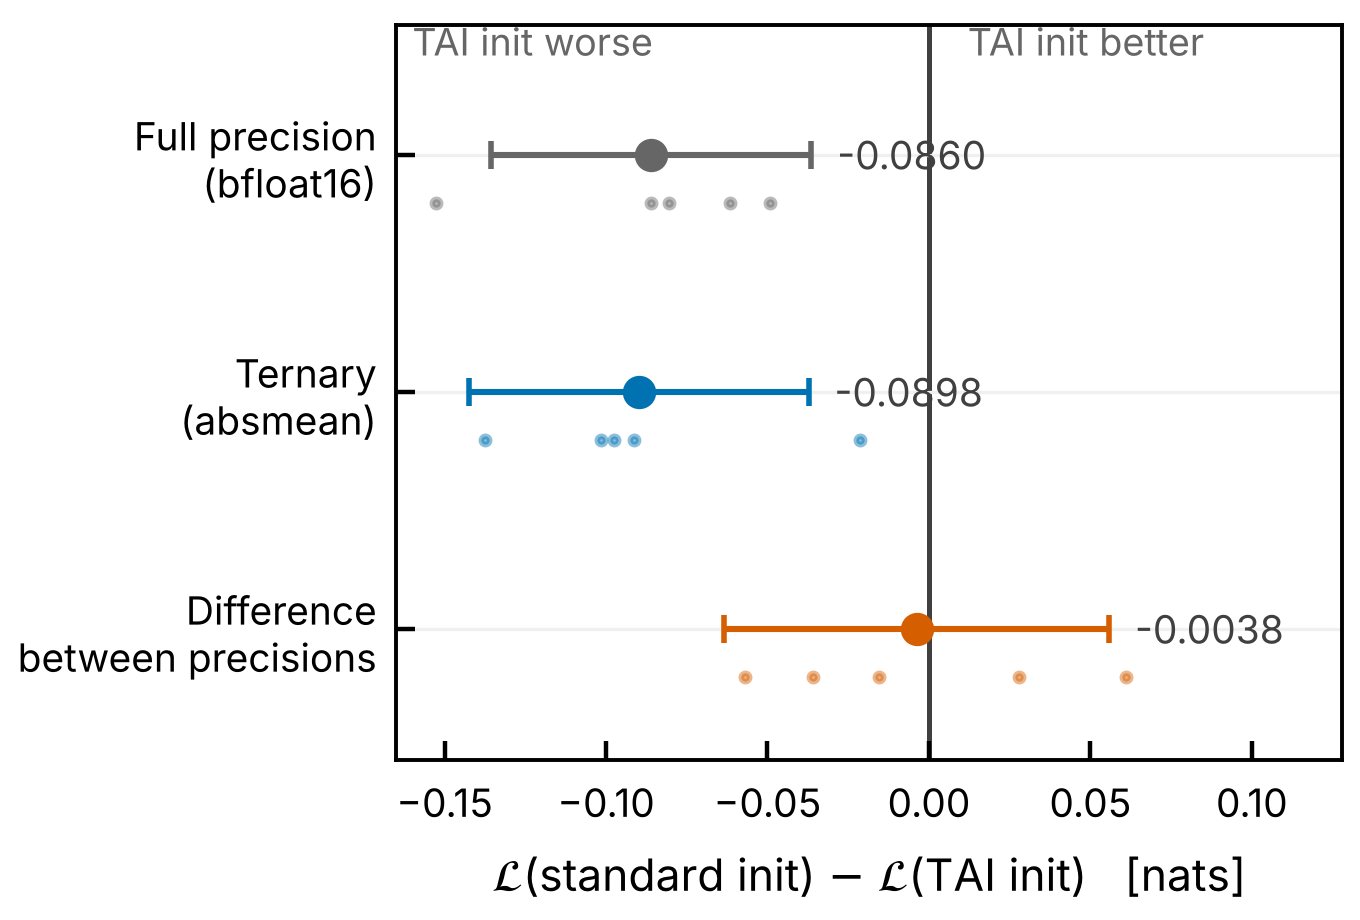
\includegraphics[width=0.8\linewidth]{fig8_init_ablation.png}
\caption{The $\{$full precision, ternary$\} \times \{$standard init, TAI
init$\}$ ablation at the primary scale ($n = 5$ seeds). Each row is the paired
initialization effect
$\mathcal{L}^{\mathrm{std\text{-}init}} - \mathcal{L}^{\mathrm{TAI\text{-}init}}$,
shown as the five per-seed values, their mean and its $95\%$ confidence
interval; negative values mean the TAI initializer attains the higher loss.
The penalty is of the same size under both precisions, and the difference
between them is indistinguishable from zero ($p = 0.869$), which is the
signature of a generically weaker initializer rather than of failed
operating-point control.}
\label{fig:initablation}
\end{figure}

The $\{$full precision, ternary$\} \times \{$standard init, TAI init$\}$ design
at the primary scale ($n = 5$ seeds) is assembled from three arms already in
the grid (\texttt{fp16\_control}, \texttt{standard} and \texttt{tai}) plus
one arm run specifically for it, \texttt{fp16\_taiinit}, which applies the TAI
initializer with quantization disabled. The design yields the initialization
effect
$\mathcal{L}^{\mathrm{std}} - \mathcal{L}^{\mathrm{TAI}}$ reported in
Table~\ref{tab:init2x2} and shown in Fig.~\ref{fig:initablation}.

\begin{table*}[t]
\centering
\small
\caption{Initialization $\times$ precision ablation at the primary scale
($n = 5$ seeds). The tabulated quantity is
$\mathcal{L}^{\mathrm{std\text{-}init}} - \mathcal{L}^{\mathrm{TAI\text{-}init}}$;
a negative value indicates that the standard initializer attains the lower
loss.}
\label{tab:init2x2}
\begin{tabular}{@{}lrr@{}}
\toprule
Precision & Initialization effect (nats) & Paired $t$-test $p$ \\
\midrule
Full precision (\texttt{bfloat16}) & $-0.0860$ & 0.0086 \\
Ternary (absmean) & $-0.0898$ & 0.0090 \\
\midrule
Difference between precisions & $-0.0038$ & 0.869 \\
\bottomrule
\end{tabular}
\end{table*}

The TAI initialization distribution carries a penalty of $0.086$ nats in full
precision and $0.090$ nats under ternary quantization. The two effects are of
the same sign, of nearly equal magnitude, and both significant at
$\alpha = 0.05$; the difference between them, $0.0038$ nats, is an order of
magnitude smaller than either, and the paired interaction contrast does not
resolve a difference ($t = +0.18$, $p = 0.869$, bootstrap 95\% CI
$[-0.035, +0.040]$); at $n = 5$ that interval is too wide to exclude an
interaction of half the size of either main effect, so what is established is
the absence of a detectable difference rather than equality. The
pre-registered discriminating pattern for
attributing the effect to operating-point control, a null effect in full
precision alongside a positive effect under quantization, is not observed:
neither leg holds, since the full-precision effect is significant and the
quantized effect runs opposite to the predicted direction.

%-----------------------------------------------------------------------------
\subsection{H6: behaviour across the scale ladder}
\label{sec:res-h6}

\begin{figure}[t]
\centering
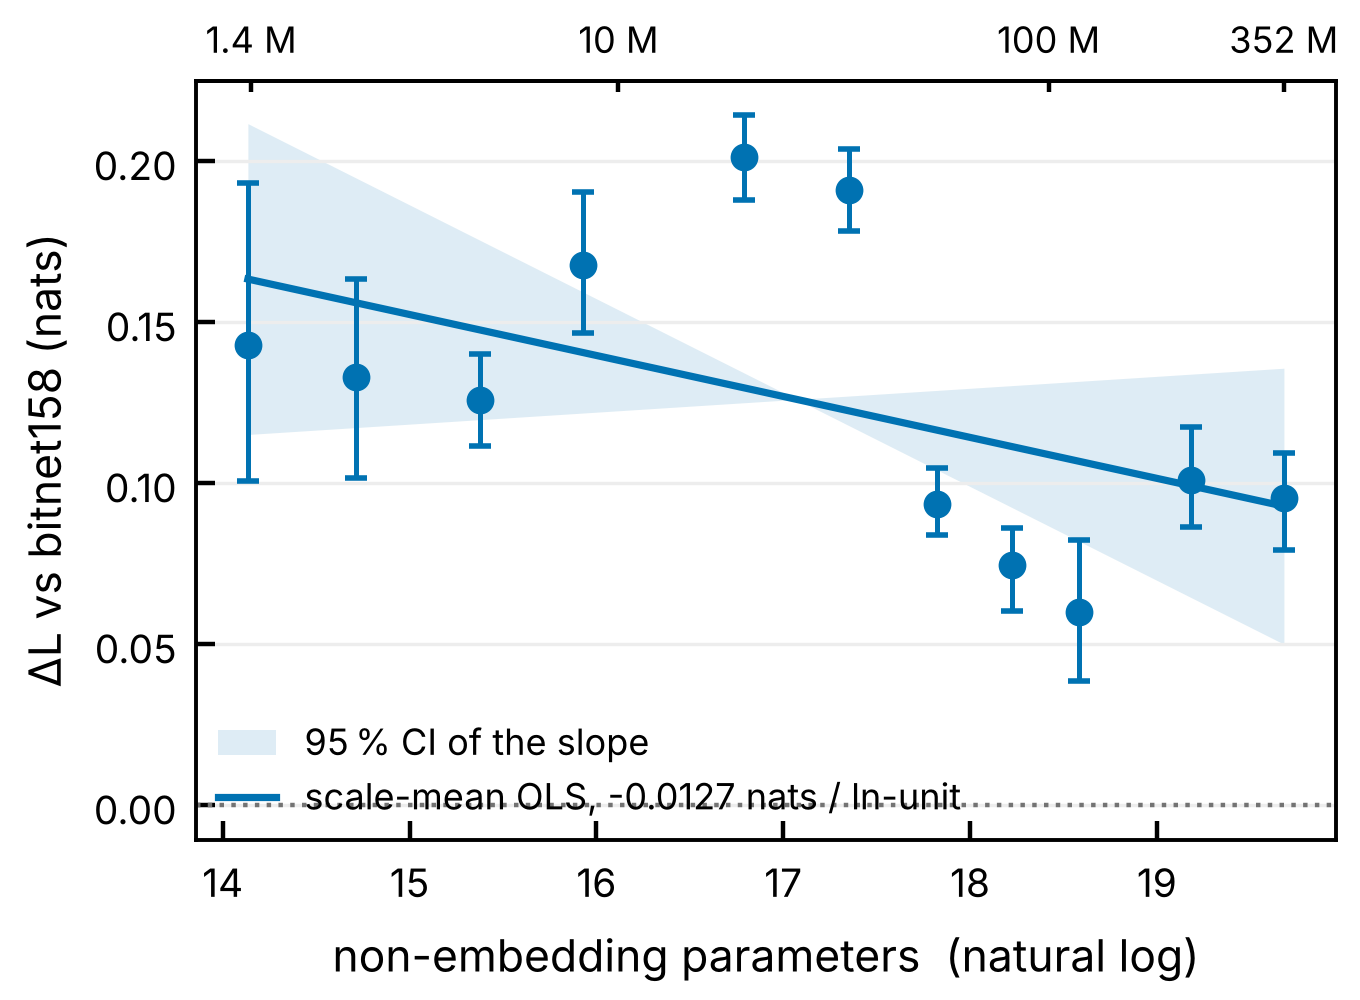
\includegraphics[width=0.86\linewidth]{fig6_scale.png}
\caption{The paired contrast of \texttt{tai\_warmup} against the
pre-registered baseline at each ladder point, with bootstrap 95\% confidence
intervals over seeds, and the primary scale-mean OLS slope of
Section~\ref{sec:res-h6} with its confidence interval. The slope is in nats
per natural log-unit of non-embedding parameters, and its interval spans zero.
The depth-controlled ladder is shown in Fig.~\ref{fig:twoslope}.}
\label{fig:scale}
\end{figure}

The primary readout is per-scale sign consistency. The effect
$\dL$ for \texttt{tai\_warmup} is positive at $11$ of $11$ ladder points
spanning $1.4$\,M to $352.3$\,M non-embedding parameters (binomial
$p = 0.0010$; Fig.~\ref{fig:scale}), with per-scale means listed in Table~\ref{tab:crossscale}. The
mean effect over scales is $+0.1260$ nats. Against the data-selected minimum
baseline, the exploratory sensitivity of Section~\ref{sec:res-h2}, the mean
effect is $+0.0818$ nats and the sign reverses at one scale.

The secondary slope diagnostic is reported with its estimator-dependence made
explicit, because the pre-registered mixed-effects model with a random
intercept per seed failed with a singular random-effects covariance, the
between-seed standard deviation of the effect being small relative to the
between-scale standard deviation. Table~\ref{tab:h6slope} reports the three
fallback estimators.

\begin{table*}[t]
\centering
\footnotesize
\caption{Slope of the \texttt{tai\_warmup} effect against $\log N$
(non-embedding parameters). The pre-registered mixed-effects estimator did not
converge. Clustering by seed treats scale-level variation as replicated within
seed and is anticonservative for a scale-level question; it is reported for
completeness only.}
\label{tab:h6slope}
\begin{tabular}{@{}llrrr@{}}
\toprule
Estimator & Unit & Slope & 95\% CI & $p$ \\
\midrule
Scale-mean OLS & scale ($n=11$) & $-0.0127$ & $[-0.0291,+0.0037]$ & 0.114 \\
Cluster-robust by scale & scale ($n=11$) & $-0.0126$ & $[-0.0236,-0.0016]$ & 0.024 \\
Cluster-robust by seed & seed ($n=15$) & $-0.0126$ & $[-0.0181,-0.0071]$ & $7.9\times 10^{-6}$ \\
Mixed-effects (pre-registered) & \multicolumn{4}{l}{failed: singular random-effects covariance} \\
\midrule
Depth-controlled ladder & scale ($n=4$) & $-0.0553$ & $[-0.0701,-0.0392]$ & n/a \\
\bottomrule
\end{tabular}
\end{table*}

All estimators agree on the point estimate ($\approx -0.0126$ nats per natural
log-unit of parameters) and on the sign: the effect narrows as scale grows. The
scale-level interval, which is the appropriate unit for a scale-level question,
spans zero under OLS and excludes zero marginally under cluster-robust
inference. The operative statement is accordingly that the direction is
consistent across scale while the magnitude is not resolved as
scale-varying. The corresponding slopes for the auxiliary outcomes, fitted with the same
scale-mean estimator against the same baseline, are $-16.47$ steps per
log-unit for steps-to-target (95\% CI $[-27.49, -5.44]$) and $-0.0056$ for the
sparsity gap (95\% CI $[-0.0093, -0.0019]$). Extrapolations from these fits are labelled as
predictions and are not treated as evidence.

One confound has to be ruled out before the slope can be read as a statement
about scale at all, since width and depth co-vary along the principal ladder.
The depth-controlled ladder
(Table~\ref{tab:widthonly}, Fig.~\ref{fig:twoslope}), in which depth is fixed at
$L=6$ and only width varies, reproduces the sign of the main-ladder slope with a
steeper magnitude ($-0.0553$, 95\% CI $[-0.0701, -0.0392]$). The narrowing
trend is therefore not an artefact of depth co-varying with width along the
principal ladder.

\begin{table*}[t]
\centering
\small
\caption{Depth-controlled (width-only) ladder, $L = 6$ fixed, $n = 5$ seeds.
Held-out loss in nats per token, mean $\pm$ SD; $\dL$ is the paired contrast of
\texttt{tai\_warmup} against \texttt{bitnet158}, following Eq.~\eqref{eq:dL}.}
\label{tab:widthonly}
\begin{tabular}{@{}lrrrr@{}}
\toprule
Scale & \texttt{standard} & \texttt{bitnet158} & \texttt{tai\_warmup} & $\dL$ \\
\midrule
\texttt{wc384} & $5.1397 \pm 0.0298$ & $5.1402 \pm 0.0304$ & $4.9710 \pm 0.0196$ & $+0.169$ \\
\texttt{wc512} & $4.9683 \pm 0.0205$ & $4.9684 \pm 0.0173$ & $4.8487 \pm 0.0283$ & $+0.120$ \\
\texttt{wc768} & $4.8489 \pm 0.0141$ & $4.9196 \pm 0.0142$ & $4.7603 \pm 0.0138$ & $+0.159$ \\
\texttt{wc1024} & $4.9382 \pm 0.0198$ & $4.9375 \pm 0.0265$ & $4.8831 \pm 0.0107$ & $+0.054$ \\
\bottomrule
\end{tabular}
\end{table*}

\begin{figure}[t]
\centering
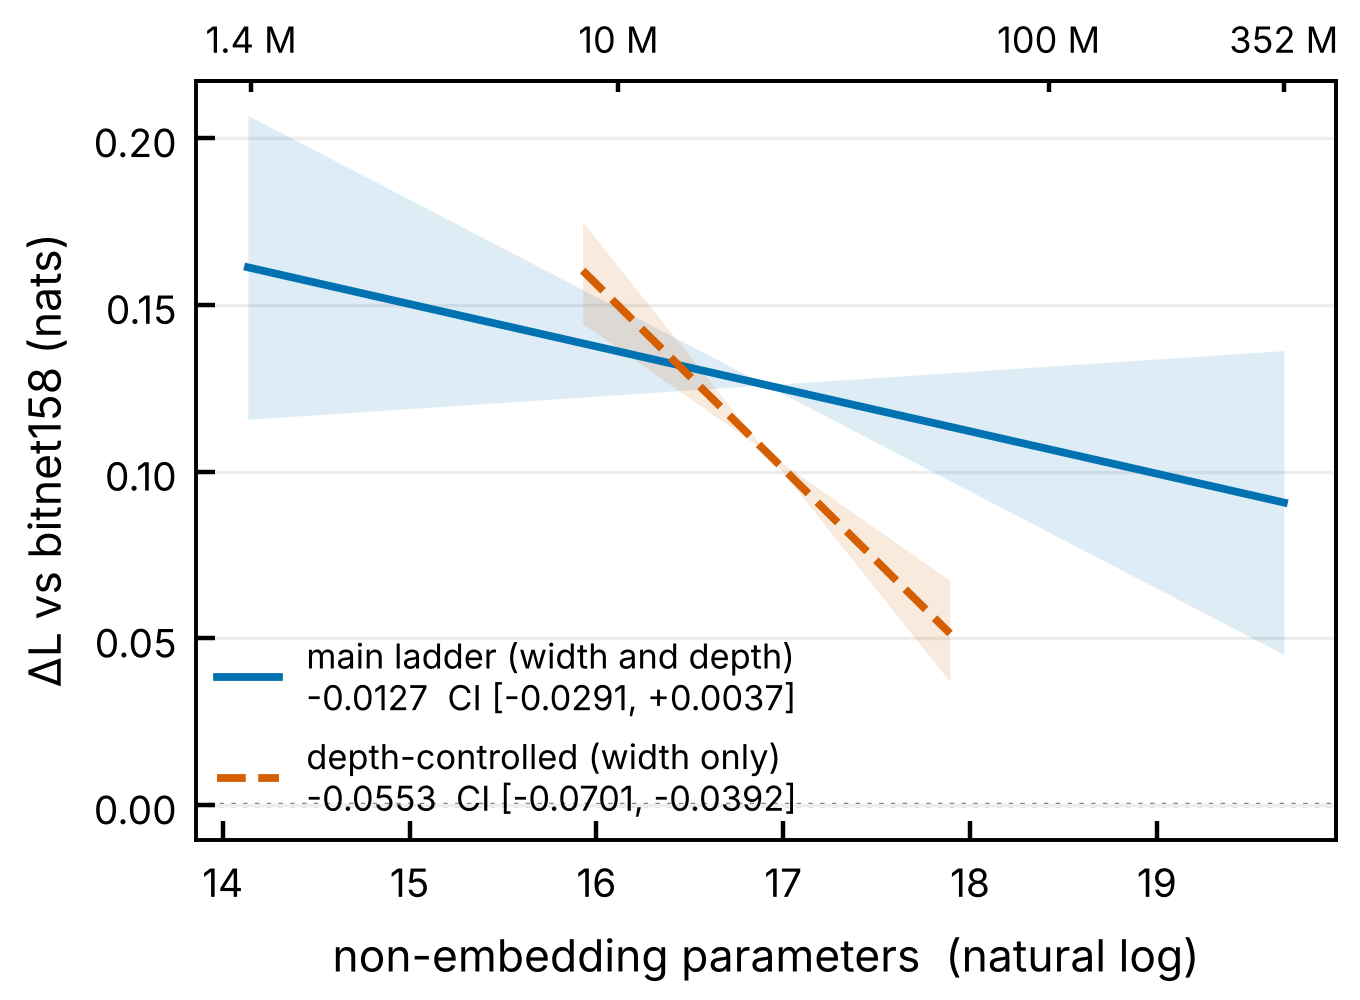
\includegraphics[width=0.86\linewidth]{fig9_two_slope.png}
\caption{Scaling slope estimated with width and depth varying together,
against the depth-controlled ladder in which depth is held fixed at $L = 6$.
Both slopes are in nats per natural log-unit of non-embedding parameters, and
each band is the $95\%$ confidence interval of its slope. The depth-controlled
fit is the steeper of the two and its interval excludes zero; the main-ladder
interval does not.}
\label{fig:twoslope}
\end{figure}

%-----------------------------------------------------------------------------
\subsection{The mechanism-matched control at its default operating point}
\label{sec:res-gammadefault}

Sections~\ref{sec:res-h3} and~\ref{sec:res-mechanism} compare
\texttt{gamma\_offset} against \texttt{tai} at matched $\rhoz$. Because
the arm also appears in the main grid at the single default $\rhoz = 0.75$, its
contrast against the pre-registered baseline is reported separately here; the
two questions have different answers and conflating them would overstate the
control.

Against \texttt{bitnet158} at the default operating point,
\texttt{gamma\_offset} attains the lower held-out loss at $7$ of the $11$
ladder points (binomial $p = 0.55$). The sign is scale-dependent and changes
once: the arm is worse at the four smallest scales (significantly so at
\texttt{dim384}, $\dL = -0.0251$, $p = 7.0\times 10^{-3}$) and better at the
seven largest, significantly at five of them, reaching $\dL = +0.0643$
($p = 1.4\times 10^{-4}$) at \texttt{dim1024} and $+0.0480$
($p = 3.1\times 10^{-4}$) at \texttt{dim1536}. A single fixed threshold
constant is therefore not uniformly preferable to the absmean convention at
this budget; the sweep of Table~\ref{tab:sweep} shows that its advantage
requires $\rhoz$ to be tuned, and that the tuned optimum itself moves with
scale ($0.70$ at \texttt{dim384}, $0.80$ at \texttt{dim768}).

\subsection{H7: transfer to a second architecture family}
\label{sec:res-h7}

Three arms were re-run on block family B (grouped-query attention with SwiGLU
feed-forward) at two scales, $15$ seeds each. For \texttt{tai\_warmup} the sign
of the effect is preserved at both: $\dL = +0.0794$
($p = 1.9\times 10^{-4}$, $n = 15$) at \texttt{dim256} and $\dL = +0.0347$
($p = 8.3\times 10^{-4}$, $n = 15$) at \texttt{dim384}.

For \texttt{gamma\_offset} at its default $\rhoz = 0.75$ the sign is
not preserved: the arm is significantly worse than the baseline on
family B at both scales, $\dL = -0.0424$ ($p = 3.7\times 10^{-3}$) at
\texttt{dim256} and $\dL = -0.0873$ ($p = 2.2\times 10^{-8}$) at
\texttt{dim384}, the latter being the largest deficit recorded for that arm
anywhere in the study. Table~\ref{tab:archB} reports both contrasts. No
$\rhoz$ sweep was executed on family B, so it is not known whether a
re-tuned threshold constant would recover the deficit; the retention property
of the threshold mechanism was likewise measured only on family A. Aggregated
over the $13$ independent (architecture $\times$ scale) cells for which a sign
is available, the effect favours \texttt{tai\_warmup} in all $13$ against the
pre-registered baseline (binomial $p = 2.4\times 10^{-4}$); against the
data-selected minimum baseline it is $12$ of $13$, the discordant cell being
\texttt{dim1024} on family A.
Magnitudes for \texttt{tai\_warmup} on family B are smaller than the
corresponding family-A values ($+0.133$ and $+0.168$ at the same two
scales).

\begin{table*}[t]
\centering
\small
\caption{Cross-architecture contrasts on block family B (GQA $+$ SwiGLU),
paired against \texttt{bitnet158} over $15$ seeds. $\dL$ follows
Eq.~\eqref{eq:dL}; positive favours the arm. Family-A values at the same scales
are reproduced from Table~\ref{tab:crossscale} and
Section~\ref{sec:res-gammadefault} for comparison.}
\label{tab:archB}
\begin{tabular}{@{}llrrr@{}}
\toprule
Scale & Arm & $\dL$ (family B) & $p_t$ & $\dL$ (family A) \\
\midrule
\texttt{dim256} & \texttt{tai\_warmup} & $+0.0794$ & $1.9\times 10^{-4}$ & $+0.1329$ \\
& \texttt{gamma\_offset} & $-0.0424$ & $3.7\times 10^{-3}$ & $-0.0032$ \\
\texttt{dim384} & \texttt{tai\_warmup} & $+0.0347$ & $8.3\times 10^{-4}$ & $+0.1677$ \\
& \texttt{gamma\_offset} & $-0.0873$ & $2.2\times 10^{-8}$ & $-0.0251$ \\
\bottomrule
\end{tabular}
\end{table*}

%-----------------------------------------------------------------------------
\subsection{H8: feedback of the sweep-optimal operating point}
\label{sec:res-h8}

Re-running the grid with $\rhoz^\star = 0.70$ as the \texttt{tai\_star} arm
($30$ runs at \texttt{dim384} and \texttt{dim768}) does not recover the deficit
of the fixed-$\rhoz$ initialization variant. At \texttt{dim384},
\texttt{tai\_star} attains $5.1919$ nats against $5.1914$ for \texttt{tai} at
$\rhoz = 0.75$, i.e.\ $\dL = -0.0805$ against the baseline; at
\texttt{dim768} it attains $5.0382$ against $5.0370$, $\dL = -0.1214$.

The comparison is not a pure change of $\rhoz$. Per-arm calibration
(Section~\ref{sec:lrcal}) gives \texttt{tai\_star} an $\eta^{\star}$ of
$2\times 10^{-3}$ at \texttt{dim384} against $3\times 10^{-3}$ for
\texttt{tai}, which is why its final sparsity ($28.4\%$) falls below the
$30.2\%$ the sweep records at the same $\rhoz = 0.70$, rather than above
\texttt{tai}'s $30.0\%$ as the monotone relation of
Section~\ref{sec:res-h3} would predict. At \texttt{dim768} the two arms
calibrate to the same rate and their sparsities agree ($29.8\%$ versus
$29.5\%$). This is also the one contrast in the study drawn across the
execution-path split of Section~\ref{sec:res-validity}, \texttt{tai\_star}
falling in the fast group at \texttt{dim384} and the baseline in the slow one;
at \texttt{dim768} both arms lie in the same group and the deficit is
unchanged, which is the comparison the conclusion rests on.

Both contrasts are significant, and for both the null is rejected under
Holm--Bonferroni within the confirmatory family. The steps-to-target deficit is reduced at \texttt{dim384}
($\dS = -35$ for \texttt{tai\_star} versus $-59$ for \texttt{tai}) and
unchanged at \texttt{dim768} ($-95$ in both). H8 is therefore not supported:
feeding back the sweep-optimal operating point neither degrades nor materially
improves the fixed-$\rhoz$ arm.

%-----------------------------------------------------------------------------
\subsection{Downstream evaluation}
\label{sec:res-downstream}

\begin{figure}[t]
\centering
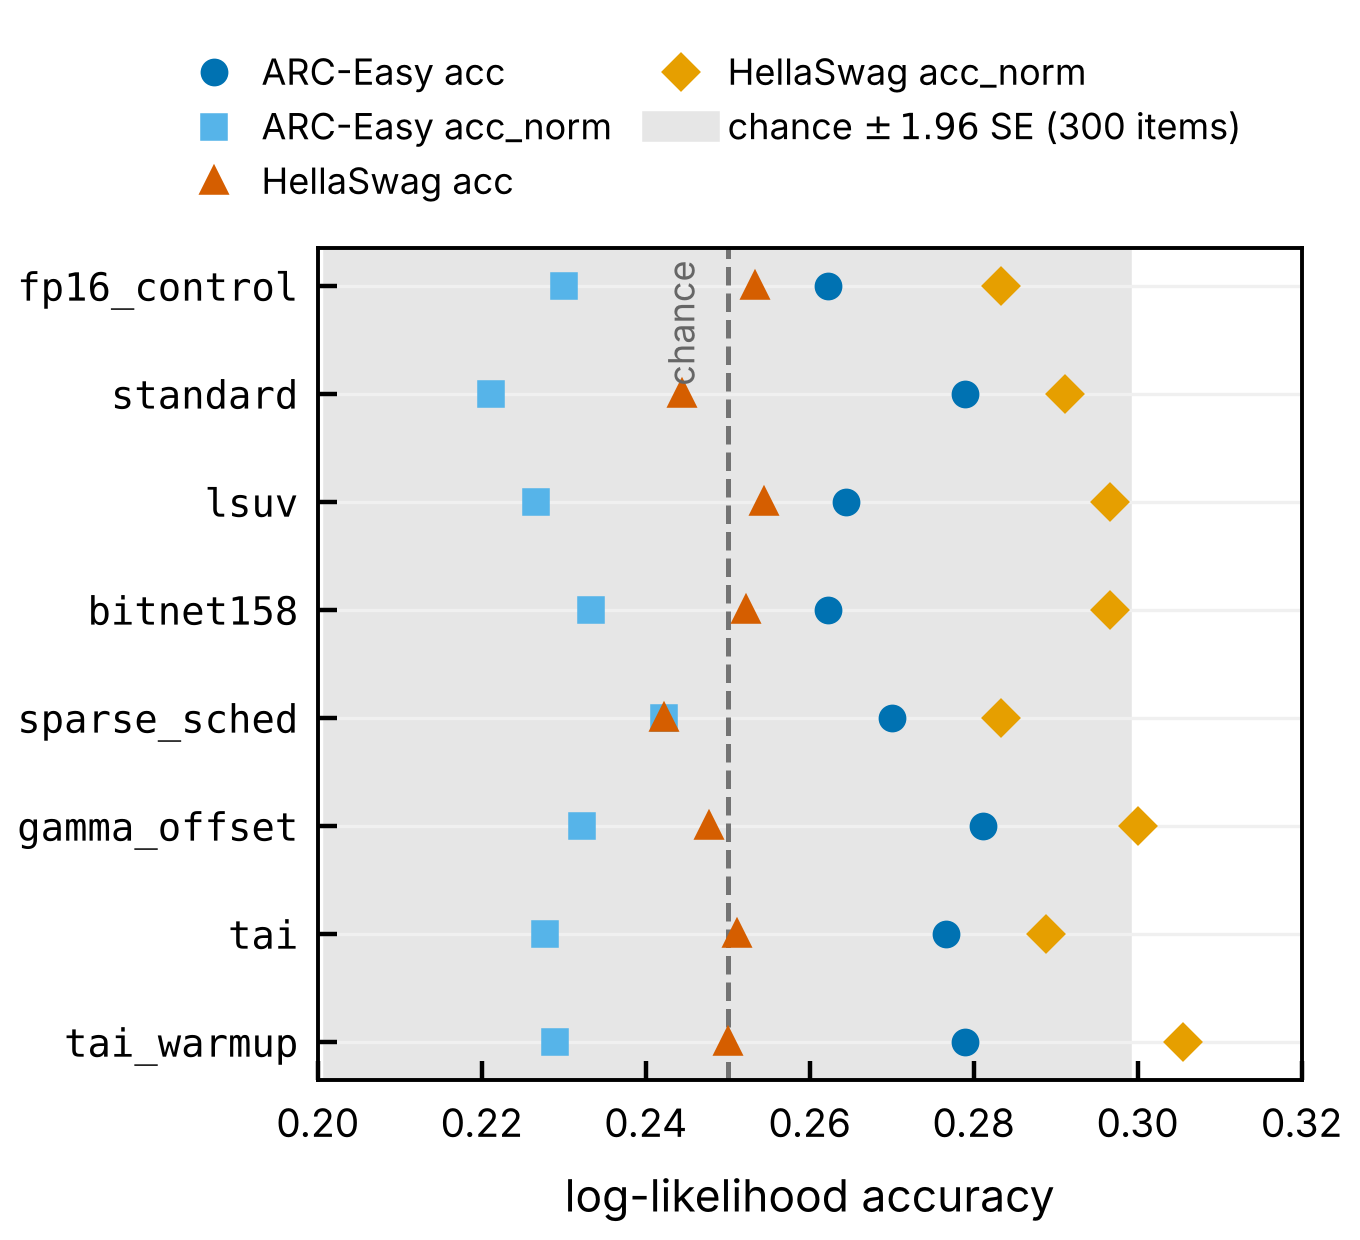
\includegraphics[width=0.9\linewidth]{fig4_lmeval.png}
\caption{Zero-shot accuracy on ARC-Easy and HellaSwag under log-likelihood
scoring, by arm, at the primary scale on the same $300$ scored items as
Table~\ref{tab:lmeval}. Both token-normalized (acc) and byte-normalized
(acc\_norm) metrics are shown. The shaded band is the random-choice rate plus
or minus $1.96$ sampling standard errors for a $300$-item subset; every
observation falls inside it.}
\label{fig:lmeval}
\end{figure}

Table~\ref{tab:lmeval} reports the four benchmark metrics at the primary
scale, and Fig.~\ref{fig:lmeval} shows them across the arm set.

\begin{table*}[t]
\centering
\small
\caption{Downstream log-likelihood accuracy at the primary scale, scored on the
first three seeds of each cell so that the comparison remains paired
($300$ items per task). $\Delta$ is the paired difference against
\texttt{bitnet158}; $p_t$ is the paired $t$-test $p$-value. Random-choice
baselines are approximately $0.25$ for both tasks.}
\label{tab:lmeval}
\begin{tabular}{@{}llrrrr@{}}
\toprule
Task / metric & Arm & Arm acc. & Baseline acc. & $\Delta$ & $p_t$ \\
\midrule
ARC-Easy (acc) & \texttt{tai} & 0.277 & 0.262 & $+0.014$ & 0.423 \\
& \texttt{tai\_warmup} & 0.279 & 0.262 & $+0.017$ & 0.138 \\
ARC-Easy (acc\_norm) & \texttt{tai} & 0.228 & 0.233 & $-0.006$ & 0.797 \\
& \texttt{tai\_warmup} & 0.229 & 0.233 & $-0.004$ & 0.673 \\
HellaSwag (acc) & \texttt{tai} & 0.251 & 0.252 & $-0.001$ & 0.921 \\
& \texttt{tai\_warmup} & 0.250 & 0.252 & $-0.002$ & 0.754 \\
HellaSwag (acc\_norm) & \texttt{tai} & 0.289 & 0.297 & $-0.008$ & 0.465 \\
& \texttt{tai\_warmup} & 0.306 & 0.297 & $+0.009$ & 0.490 \\
\bottomrule
\end{tabular}
\end{table*}

No benchmark contrast is significant at any scale after correction, and the
observed differences ($|\Delta| \leq 0.025$) are of the order of the sampling
noise of a $300$-item subset, $\sqrt{p(1-p)/300} \approx 0.025$ at the
random-choice rate. Absolute
accuracies lie between $0.21$ and $0.31$ across all arms, tasks and metrics,
i.e.\ at or marginally above the random-choice baseline. Aggregated over the
$88$ benchmark contrasts computed across the ladder, three reach nominal
$p < 0.05$, which is consistent with the number expected by chance.

The internal transfer proxy is the sole downstream measure that discriminates
between arms. Next-token top-1 accuracy at the primary scale is $0.242$ for
\texttt{tai\_warmup} against $0.227$ for the baseline
($p < 10^{-4}$) and $0.221$ for \texttt{tai} ($p < 10^{-4}$); the ordering of
these three arms matches their held-out loss ordering at every scale.

%-----------------------------------------------------------------------------
\subsection{Ablations}
\label{sec:res-ablations}

\subsubsection{Realization map of the TAI construction}

The separation condition of Lemma~\ref{lem:separation} was probed over a
$5 \times 3$ grid in the dormant magnitude $\delta$ and jitter half-width $a$
at target $\rhoz = 0.75$. In $11$ of $15$ cells the condition holds and the
target is realized to $|\rho_{\mathrm{real}} - \rhoz| \leq 1.3\times 10^{-4}$,
independently of $(\delta, a)$; in the remaining four cells
($\delta = 0.45$ at every $a$, and $\delta = 0.35$ with $a = 0.30$) the
assertion fires and the target is not realizable. The boundary is thus located
empirically and matches the analytical prediction, and the operating defaults
$(\delta, a) = (0.15, 0.15)$ sit in the interior of the valid region.

\subsubsection{Quality sensitivity to the dormant magnitude}

Although $\rho_{\mathrm{real}}$ is invariant to $\delta$ within the valid
region, final quality is not. At fixed $\rhoz = 0.75$ and $n = 5$ seeds, mean
held-out loss falls monotonically from $5.2304 \pm 0.0466$ at $\delta = 0.05$
to $5.1048 \pm 0.0202$ at $\delta = 0.35$, a spread of $0.126$ nats
(one-way ANOVA $F = 12.11$, $p = 2.2\times 10^{-4}$; exploratory, outside the
Holm family). The construction therefore exposes a second effective degree of
freedom whose influence on quality is comparable in magnitude to the
$\rhoz$ effect itself.

\subsubsection{$\gamma$-warmup schedule grid}

The $3 \times 3$ grid over warmup start $s_0$ and duration $\tau_w$ at the
primary scale ($n = 5$ seeds) is reported in Table~\ref{tab:warmupgrid}.
The best cell is $(s_0, \tau_w) = (0.4, 120)$ at $5.0437$ nats and the worst
is $(0.5, 480)$ at $5.1838$; loss increases monotonically in $\tau_w$ at every
$s_0$, and $s_0 = 0.5$ is dominated by $s_0 = 0.4$ at every $\tau_w$. The
grid-default configuration used in the main grid, $(0.4, 240)$, is the second-best cell ($5.0514$).

\begin{table}[t]
\centering
\small
\caption{$\gamma$-warmup ablation at the primary scale (\texttt{dim384}): mean
held-out loss in nats per token over $5$ seeds, as a function of the warmup
start $s_0$ and the duration $\tau_w$ in optimizer steps.}
\label{tab:warmupgrid}
\begin{tabular}{@{}lrrr@{}}
\toprule
$s_0 \backslash \tau_w$ & 120 & 240 & 480 \\
\midrule
0.3 & 5.0536 & 5.1249 & 5.1564 \\
0.4 & \textbf{5.0437} & 5.0514 & 5.1130 \\
0.5 & 5.1553 & 5.1568 & 5.1838 \\
\bottomrule
\end{tabular}
\end{table}

\subsubsection{Learning-rate sensitivity}

Across the five-point learning-rate grid at the primary scale
(Table~\ref{tab:lrsens}), \texttt{tai\_warmup} attains the lower loss at four
of five settings; the ordering reverses only at the smallest rate
($5\times 10^{-4}$), where both arms are far from their optima. At the baseline's own
optimum ($3\times 10^{-3}$), where the comparison is least favourable to
\texttt{tai\_warmup}, the advantage is $0.218$ nats, and it is larger still at
$5\times 10^{-3}$ ($0.250$). The reported conclusion is therefore not an artefact of a single
optimizer setting.

\begin{table}[t]
\centering
\small
\caption{Learning-rate sensitivity at the primary scale (\texttt{dim384},
$n = 5$ ablation seeds). Entries are mean held-out loss $\mathcal{L}$ in
nats/token; $\dL$ is the paired contrast against \texttt{standard}, the
comparison arm of this ablation, so positive favours
\texttt{tai\_warmup}. The baseline's minimum over the grid ($5.1196$ at
$3\times 10^{-3}$) is interior and therefore a genuine envelope;
\texttt{tai\_warmup} falls below it at the three largest rates, which excludes
the global effective-learning-rate account of the schedule
(Section~\ref{sec:disc-timing}).}
\label{tab:lrsens}
\begin{tabular}{@{}lrrr@{}}
\toprule
Peak LR & \texttt{standard} & \texttt{tai\_warmup} & $\dL$ \\
\midrule
$5\times 10^{-4}$ & 5.7185 & 5.8034 & $-0.085$ \\
$1\times 10^{-3}$ & 5.4115 & 5.3928 & $+0.019$ \\
$2\times 10^{-3}$ & 5.1893 & 5.0409 & $+0.148$ \\
$3\times 10^{-3}$ & 5.1196 & 4.9019 & $+0.218$ \\
$5\times 10^{-3}$ & 5.1891 & 4.9390 & $+0.250$ \\
\bottomrule
\end{tabular}
\end{table}

%-----------------------------------------------------------------------------
\subsection{Efficiency}
\label{sec:res-eff}

Table~\ref{tab:efficiency} separates the theoretical deployment model from the
measured simulation cost, in the order specified by the protocol.

\begin{table*}[t]
\centering
\scriptsize
\caption{Efficiency. Panel (A) is a counting argument over the ternary codebook
at the largest \emph{declared} configuration, \texttt{dim2048}, which was not
executed (Section~\ref{sec:res-validity}); the compression ratios do not depend
on the parameter count, so only the absolute sizes are specific to it. It is
independent of the hardware used here.
Panel (B) is the measured cost of simulating ternary arithmetic in
\texttt{bfloat16} under straight-through estimation; it is a property of the
research harness and is not a ternary-inference measurement. No ternary kernel
was benchmarked in this work.}
\label{tab:efficiency}
\begin{tabular}{@{}lrr@{}}
\toprule
\multicolumn{3}{@{}l}{\textbf{(A) Deployment model (theoretical, primary)}} \\
\midrule
Quantized parameters & \multicolumn{2}{r}{782.91\,M} \\
Half-precision size & \multicolumn{2}{r}{1493.28\,MB} \\
Ternary size, information-theoretic ($\log_2 3 = 1.585$ bits/weight) & \multicolumn{2}{r}{147.92\,MB} \\
Ternary size, 2-bit packed & \multicolumn{2}{r}{186.66\,MB} \\
Compression vs.\ half precision (information-theoretic) & \multicolumn{2}{r}{$10.09\times$} \\
Compression vs.\ half precision (2-bit packed) & \multicolumn{2}{r}{$8.00\times$} \\
\midrule
\multicolumn{3}{@{}l}{\textbf{(B) Simulation cost (measured, secondary)}} \\
\midrule
& \texttt{fp16\_control} & ternary (simulated) \\
Latency & 430.9\,ms & 718.9\,ms \\
Throughput & 38{,}025 tok/s & 22{,}792 tok/s \\
Peak memory & 3.336\,GB & 3.336\,GB \\
Forward sparsity & 0.0\% & 25.0\% \\
Latency ratio & \multicolumn{2}{r}{$1.67\times$} \\
\bottomrule
\end{tabular}
\end{table*}

The simulated ternary path is $1.67\times$ slower than the full-precision
control at identical peak memory, which is the expected direction: under
straight-through estimation the ternary path executes the same
\texttt{bfloat16} matrix multiplication and additionally performs
normalization, activation quantization, weight quantization and rescaling,
while retaining \texttt{bfloat16} master weights. This quantity is charged
honestly to the method in the compute-equal accounting and carries no
deployment implication in either direction.

%-----------------------------------------------------------------------------
\subsection{Summary of pre-registered outcomes}
\label{sec:res-summary}

Table~\ref{tab:hypsummary} consolidates the outcome of each pre-registered
hypothesis under the wording licensed by Section~\ref{sec:res-budget}.

\begin{table*}[t]
\centering
\scriptsize
\caption{Outcome of every pre-registered hypothesis. Token-equal indicates
that the claim is restricted to performance at the fixed $20$\,M-token budget,
convergence not having been established for any arm.}
\label{tab:hypsummary}
\begin{tabular}{@{}p{0.9cm}p{2.7cm}p{6.1cm}@{}}
\toprule
Hyp. & Outcome & Operative statement \\
\midrule
H1 & Split &
Supported for \texttt{tai\_warmup} ($11/11$ scales, $\dS$ up to $+148$ steps);
rejected in the opposite direction for \texttt{tai} ($11/11$ scales slower). \\
\addlinespace
H2 & Untestable (pre-reg.) &
No run reached plateau ($0/760$); the convergence-conditional equivalence test
has an empty qualifying set. The token-equal companion returns
\texttt{tai\_warmup} superior at $11/11$ scales and \texttt{tai} inferior at
$10/11$; equivalence is never returned. \\
\addlinespace
H3 & Not supported (strong form) &
Ordinal control is near-perfect (per-seed Spearman $-0.996$, SNR $44.9\times$)
and the placebo is flat, but retention for the initialization mechanism is
$0.052$--$0.069$: $93$--$95\%$ of the intervention is erased, and final
sparsity converges to an attractor near $0.30$. The threshold-offset mechanism
retains $1.003$--$1.006$. \\
\addlinespace
H4 & Supported &
No evidence of variance inflation on the pooled seed $\times$ fold matrix
($W = 0.554$, $p = 0.458$); $23/24$ per-cell Levene tests are non-significant
and the one exception favours lower TAI variance. \\
\addlinespace
H5 & Supported for the threshold mechanism &
The threshold-offset arm traces a U-shaped frontier spanning $50$ points of
sparsity with an interior optimum; the initialization arm's sparsity axis spans
$2.6$ points, rendering its frontier near-degenerate.
$\rhoz^\star = 0.70$ (bootstrap $P = 0.758$). \\
\addlinespace
H6 & Direction supported; magnitude unresolved &
Sign positive at $11/11$ scales (binomial $p = 0.0010$) over $1.4$\,M--$352$\,M
parameters. Slope $-0.0127$ per log-unit under the scale-level OLS estimator,
whose interval spans zero. The depth-controlled ladder reproduces the sign. \\
\addlinespace
H7 & Supported for \texttt{tai\_warmup}; not for \texttt{gamma\_offset} &
Sign preserved for \texttt{tai\_warmup} on family B at both tested scales
($p \leq 8.3\times 10^{-4}$); all $13$ architecture $\times$ scale cells
consistent against the pre-registered baseline (binomial
$p = 2.4\times 10^{-4}$), $12/13$ against the data-selected minimum. \texttt{gamma\_offset} at its default
$\rhoz$ is significantly worse than the baseline on family B at both scales
(Table~\ref{tab:archB}). \\
\addlinespace
H8 & Not supported &
\texttt{tai\_star} at $\rhoz^\star = 0.70$ tracks \texttt{tai} to within
$0.0013$ nats at both tested scales and remains below the baseline. \\
\bottomrule
\end{tabular}
\end{table*}

Two auxiliary controls complete the picture. The mechanism-matched contrast
places the quality difference in \texttt{gamma\_offset}'s favour at
$0.0610$ nats, 95\% CI $[+0.0474, +0.0742]$, over $90$ paired cells at matched
$\rhoz$, though, as Sections~\ref{sec:res-gammadefault} and~\ref{sec:res-h7}
record, that arm's advantage over the baseline is scale-dependent on
family A and reverses on family B. The $2 \times 2$ ablation finds the TAI
initialization distribution to carry an almost identical penalty in full
precision ($-0.086$ nats) and under quantization ($-0.090$ nats), so the
pre-registered pattern that would attribute the effect to ternary
operating-point control is not observed.

Taken together, the results separate cleanly into three groups: what the
initialization intervention does (little, and durably almost nothing), what the
threshold intervention does (everything the initialization was supposed to do,
with caveats of its own), and what annealing the threshold does (the largest
and most consistent effect in the study). Section~\ref{sec:discussion} takes
each group in turn and asks why the quantizer's own definition makes this
separation almost inevitable.

%=============================================================================

%=============================================================================

\section{Discussion}
\label{sec:discussion}

%-----------------------------------------------------------------------------
\subsection{What the experiment establishes, and what it does not}
\label{sec:disc-summary}

It is worth stating plainly, and early, that this study did not confirm the
hypothesis it was designed to confirm. The pre-registered claim was that
shaping the initial weight-magnitude distribution so as to place a ternary
network at a chosen operating point $\rhoz$ would improve both convergence
speed and final quality, and would causally determine the sparsity the network
eventually learns. Of these, the first is supported only for the schedule
variant, the second is reversed for the fixed-$\rhoz$ variant, and the third is
supported for a mechanism that is not the proposed one. The value of the work
lies in the sharpness with which the design separates these outcomes, and we
have organised the discussion around that separation rather than around a
defence of the original claim.

Three findings survive scrutiny, and they are of unequal importance.

First, and least contentious: the ternary operating point is analytically
locked and the lock is real. For any zero-mean initializer, the absmean rule
places the network at $\rhoz = 0.6899$ irrespective of the initialization
scale, and the measurement confirms this across two orders of magnitude in
$\sigma$, over which the empirical active fraction varies by $6\times10^{-4}$,
and across four initializer families, all of which land within $10^{-3}$ of
the analytical value (Table~\ref{tab:locked}). This is a small analytical observation, but it has a
practical consequence that the quantization literature has not made explicit:
in an absmean ternary network, initialization scale is not a lever on sparsity,
and any study that varies $\sigma$ hoping to trade quality against density is
varying nothing.

Second, and most important: the two mechanisms that can move the
operating point behave completely differently under training. The threshold
offset \texttt{gamma\_offset} retains its target essentially perfectly ($r = 1.003$ and $1.006$ at the two
tested scales, $R^{2} = 1.000$); an initialization intervention of identical
nominal magnitude is almost entirely erased ($r = 0.052$ and $0.069$). A
$50$-percentage-point manipulation of initial sparsity leaves $50$ points of
final sparsity in the first case and between $2.6$ and $3.6$ points in the
second. We regard this contrast, rather than the performance of any single
arm, as the central empirical result of the paper, and Section~\ref{sec:disc-attractor} is devoted to why it arises.

Third: annealing the threshold works, and does so consistently. The
$\gamma$-warmup arm \texttt{tai\_warmup} attains a lower held-out loss
$\mathcal{L}$ and reaches its scale's pre-registered target loss
($\mathcal{L}_{\mathrm{target}} = 5.6539$ at the primary scale) in fewer steps
than the frozen primary baseline \texttt{bitnet158} at $11$ of $11$ scales
spanning $1.4$\,M--$352$\,M non-embedding parameters, at all $13$
architecture~$\times$~scale cells, and at four of five learning rates. The
effect is not fragile with respect to seed, fold, architecture family, depth,
or optimizer setting. Whether it is fragile with respect to training
budget is the principal open question, and we treat it at length in
Section~\ref{sec:disc-budget}.

Against these, three pre-registered claims failed, and the reasons are
instructive rather than merely negative: the fixed-$\rhoz$ initializer
\texttt{tai} is a worse initializer in full precision as well as under
quantization (Section~\ref{sec:disc-attribution}); the mechanism-matched
control \texttt{gamma\_offset} outperforms it at matched $\rhoz$
(Section~\ref{sec:disc-attribution}); and the feedback of the sweep-optimal
operating point, \texttt{tai\_star}, had almost no room to change anything, for
reasons that are a consequence of the retention result itself
(Section~\ref{sec:disc-designcritique}).

One qualification must be carried through everything that follows, because it
bounds the strongest reframing these data will support. That
\texttt{gamma\_offset} beats \texttt{tai} at matched $\rhoz$ is robust
($+0.0610$ nats, $95\%$ CI $[+0.0474,+0.0742]$, $90$ paired cells). That
\texttt{gamma\_offset} beats the baseline is not a general fact: at its
default $\rhoz = 0.75$ it does so at only seven of eleven scales on family~A,
with the sign turning over mid-ladder, and it is significantly worse
than the baseline on family~B at both tested scales
(Section~\ref{sec:res-h7}). The durability of the threshold mechanism and the
competitiveness of any particular threshold constant are separate claims, and
only the first is established here.

%-----------------------------------------------------------------------------
\subsection{Why the initialization intervention is erased: the absmean
attractor}
\label{sec:disc-attractor}

The retention asymmetry has a straightforward explanation, and articulating it
is the main theoretical contribution we can defend.

The absmean threshold is not an external constant. It is a functional of the
weight matrix itself,
\begin{equation}
\label{eq:selfref}
\gamma(\Wm; c) \;=\; c\,\E|w|,
\end{equation}
so the criterion by which a weight is judged large enough to survive moves
whenever the weight distribution moves. An initialization intervention perturbs
the numerator and the denominator of the same ratio: TAI shapes $|w|$ into two
modes, but $\E|w|$ is computed from those same modes, and the surviving
fraction is determined only by where the modes sit relative to their own
mean. Gradient descent then acts on the weights, and as it does so it drags
$\gamma$ along with them. The threshold is, in this precise sense, adaptive;
nothing in the training dynamics preserves the initial partition, and the
system relaxes to whatever active fraction the optimizer's own steady-state
magnitude distribution implies.

The measurements are consistent with exactly this picture. The fitted fixed
point of the retention regression is $0.305$ at \texttt{dim384} and $0.300$ at
\texttt{dim768}, and the untouched \texttt{standard} arm lands at $0.321$ and
$0.318$ respectively. All four straddle the analytical initialization value
$1 - \rhoz = 0.310$ within $0.011$, the fitted attractors falling just below
it and the untouched arm just above. In other words, the value
$\approx 0.31$ that Proposition~\ref{prop:locked} identifies as a property of
initialization turns out to be approximately where the optimizer goes
anyway. This reframes the premise of the paper in a way we did not anticipate:
the locked operating point is not merely a shared default that every zero-mean
initializer happens to inherit; it is close to an attractor of ternary training
under this quantizer.

A threshold offset escapes this because it changes the constant $c$, which no
gradient touches. The survival condition $|w| \geq \tfrac{c}{2}\E|w|$ is
homogeneous of degree zero in the weights, so rescaling the weights cannot undo
a change in $c$; only a change in the shape of the magnitude
distribution could, and the observed $R^{2} = 1.000$ indicates that shape
change is negligible over the tested range. The consequence is a clean
prediction that we did not test and that a follow-up study should:
any quantizer whose threshold is a fixed multiple of a
distribution statistic of the current weights will exhibit low retention of
initialization interventions, while any quantizer whose threshold is constant
in the weights will retain them. Trained ternary quantization
\cite{zhu2017a} falls on the first side of this line despite learning its
per-layer scaling factors, because its threshold is a fixed multiple of
$\max|w|$ and therefore moves with the weights exactly as the absmean rule
does. The result reported
here is therefore not about TAI specifically but about the class of
self-referential thresholds to which absmean and BitNet~b1.58
\cite{ma2024} belong.

There is an important edge case. Retention was measured over
$\rhoz \in [0.4, 0.9]$, i.e.\ initial sparsity in $[0.10, 0.60]$. We do not
know whether the attractor persists at extreme operating points, at, say,
$90\%$ sparsity, where the surviving weights are few enough that the mean
absolute weight is dominated by the dormant mass and the feedback in
Eq.~\eqref{eq:selfref} may behave differently. The claim is bounded to the
tested range.

%-----------------------------------------------------------------------------
\subsection{Timing rather than distribution, and an honest confound}
\label{sec:disc-timing}

The single largest effect in the study is not an initialization effect at all.
It is the $\gamma$-warmup schedule of \texttt{tai\_warmup}, which lowers the
threshold early, raising the active fraction above its locked value, and
relaxes the threshold to the nominal $c = 1$ over $\tau_w$ steps. This arm improves on
\texttt{bitnet158} by $0.060$ to $0.201$ nats depending on scale, whereas the
fixed-$\rhoz$ initializer \texttt{tai} falls short of it by $0.052$ to
$0.120$ nats. Same target operating point,
opposite outcome; the difference is when the network is required to be there.

The ablation is consistent with a transient-density reading. Loss increases
monotonically in $\tau_w$ at every warmup start, and the best configuration is
the one with the shortest warmup at an intermediate start,
$(s_0, \tau_w) = (0.4, 120)$; the least aggressive start, $s_0 = 0.5$, is the
worst at every duration.
That is, the benefit comes from a brief early period in which more weights
carry non-zero ternary codes, and therefore more weights receive a non-zero
contribution through the straight-through estimator \cite{bengio2013}, not
from a prolonged departure from the nominal threshold. The natural mechanistic
story is that early ternary training is gradient-starved: roughly $31\%$ of
weights are quantized to zero at initialization, and a temporarily denser
forward pass lets the network establish useful structure before the threshold
tightens.

We must, however, flag a confound that a referee will raise and that our data
cannot fully dispel. Scaling $\gamma$ down by $s_0$ scales the magnitude of the
quantized weights by the same factor, which scales the forward activations and,
through the straight-through path, the effective gradient magnitude of every
BitLinear layer. A $\gamma$-warmup is therefore not only a sparsity
schedule; it is also, in part, an implicit rescaling of the network's effective
learning rate during exactly the period when the explicit learning-rate warmup
is active. The coincidence is uncomfortably exact: the best warmup duration
found by ablation, $\tau_w = 120$ steps, is precisely the length of the
learning-rate warmup fixed in the protocol. We do not think this fully explains
the effect. The learning-rate sensitivity ablation shows the advantage
persisting, and indeed growing, at the upper four of the five peak learning
rates tested, reversing only at $5\times 10^{-4}$ where both arms are far from
their optima; an implicit-learning-rate account would not naturally predict
that pattern. The same ablation excludes the simplest form of the confound
outright.

The exclusion is an envelope argument. If $\gamma$-warmup acted purely as a
multiplier on the effective learning rate, then every outcome it can reach
would also be reachable by the baseline at some other learning rate: the set of
achievable losses would be a subset of the baseline's learning-rate curve, and
the schedule could not beat that curve's minimum. It does. At the primary
scale the baseline's loss over the five-point grid is $5.7185$, $5.4115$,
$5.1893$, $5.1196$ and $5.1891$ nats, an interior minimum of $5.1196$ that is
bracketed on both sides and therefore a genuine envelope rather than a
truncated one. The $\gamma$-warmup arm falls below that envelope at three of
the five learning rates (by $0.079$ nats at $2\times 10^{-3}$, $0.218$ at
$3\times 10^{-3}$ and $0.181$ at $5\times 10^{-3}$), reaching $4.9019$ nats at
its own optimum. No reparameterization of a single global learning rate can
produce a loss the baseline cannot attain at any learning rate, so the
account of $\gamma$-warmup as an implicit learning-rate schedule is refuted
in its global form.

What the argument does not exclude is a gradient-scale effect that is
time-varying or layer-dependent, since such an effect is not equivalent to any
single global rate. Settling that requires the control we specify in
Section~\ref{sec:disc-future}: a matched arm holding the threshold at $c = 1$
while rescaling the BitLinear output by the same $g_{\mathrm{warm}}(t)$,
reproducing the gradient-scale trajectory with no change to the sparsity
schedule.

A second observation belongs here because it is easy to over-read. The
gradual-pruning baseline \texttt{sparse\_sched}, which drives the threshold in
the opposite direction, is the weakest ternary baseline at the primary scale. It is tempting to
present this as a clean mirror image (annealing down helps, annealing up
hurts), but the comparison is confounded: the gradual-pruning arm terminates at
$c = 1.6$ and $48.8\%$ sparsity, whereas $\gamma$-warmup terminates at $c = 1$
and $30.3\%$. Its deficit therefore conflates schedule direction with terminal
operating point, and at least part of it is simply the quality cost of ending
$18$ points sparser. The honest statement is that we did not test annealing
direction with the terminal point held fixed.

%-----------------------------------------------------------------------------
\subsection{Attribution: the contribution is about $\gamma$, not about $\Wm$}
\label{sec:disc-attribution}

Two controls, both pre-registered and both designed so that the proposed method
could lose, agree that the initialization distribution is not where the benefit
lives.

The $2\times 2$ initialization~$\times$~precision ablation is the more decisive
of the two. Had TAI's advantage derived from control of the ternary operating
point, the initializer should have been neutral in full precision, where there
is no threshold to control, and beneficial under quantization. The measured
pattern is neither: the TAI distribution costs $0.086$ nats in full precision
and $0.090$ nats under ternary quantization, effects of the same sign, nearly
equal magnitude, and comparable significance, differing by $0.0038$ nats, an
order of magnitude less than either. The parsimonious reading is that the
two-point magnitude law is simply a worse initializer, in the ordinary sense in
which initializers are better or worse \cite{glorot2010,he2015},
and that its cost is paid identically whether or not the weights are
subsequently ternarized.

The dormant-magnitude ablation supports this and supplies a mechanism. Within the region where the separation condition of
Lemma~\ref{lem:separation} holds, the realized $\rhoz$ is exactly on target and
completely independent of the dormant magnitude $\delta$, yet quality is not:
loss falls monotonically from $5.2304$ at $\delta = 0.05$ to $5.1048$ at
$\delta = 0.35$, a spread of $0.126$ nats, which is comparable to the entire
$\rhoz$ effect over the sweep. Since increasing $\delta$ toward the active
magnitude $\alpha$ makes the distribution progressively less bimodal, quality
improves monotonically as the TAI construction is deformed toward a unimodal
distribution, that is, toward the standard initializer it was meant to
replace. Two facts follow that the paper must state rather than bury: TAI
possesses a second, quality-relevant degree of freedom that is not the
operating point, so the framing of $\rhoz$ as the knob is incomplete; and the
direction in which that knob helps points away from the method.

The mechanism-matched control closes the argument from the other side. Paired
over $90$ $(\rhoz, \mathrm{seed})$ cells, \texttt{gamma\_offset} attains a loss
$0.0610$ nats lower than \texttt{tai}, $95\%$ CI $[+0.0474, +0.0742]$, and it
retains the operating point essentially perfectly while \texttt{tai} does not.
Of the three readings we pre-registered for this contrast, the outcome is the
one in which the simpler mechanism wins on both axes on which the two were
designed to be compared.

The finding must not be over-read. It concerns two ways of reaching the
same operating point, and does not establish that a
constant threshold offset is a better ternary recipe than the absmean
convention. The evidence there is mixed and in one place negative: at its
default $\rhoz$, \texttt{gamma\_offset} beats \texttt{bitnet158} at seven of
eleven family-A scales with the sign turning over mid-ladder
(Section~\ref{sec:res-gammadefault}), and it is significantly worse on family~B
at both tested scales, by $-0.042$ and $-0.087$ nats
(Section~\ref{sec:res-h7}). Two readings are available and these data do not
separate them: either the optimal constant is architecture-dependent (which is
plausible, since the sweep already shows it to be scale-dependent, moving from
$\rhoz^{\star} = 0.70$ at \texttt{dim384} to $0.80$ at \texttt{dim768}) or the
permanent rescaling of the quantized weight magnitudes, and hence of the
effective gradient scale, that a fixed $c \neq 1$
imposes interacts badly with the gated feed-forward block of family~B. No
$\rhoz$ sweep was executed on family~B, so this is an open question rather than
a resolved one. What survives unqualified is the narrower and more durable
claim: if an operating point is to be held, the threshold holds it and
the initializer does not.

The contribution is therefore best stated as follows: the ternary
operating point is analytically locked under every standard initializer; it can
be unlocked, but only a threshold intervention unlocks it durably; and
annealing that threshold, rather than displacing the initial weight
distribution, is what improves training. The initializer is the vehicle by
which we discovered this, and reporting its failure is what makes the
threshold result credible.

%-----------------------------------------------------------------------------
\subsection{Relation to prior work}
\label{sec:disc-prior}

We relate the results to four lines of work: the ternary quantizers whose
thresholds we reparameterize, the initialization literature whose framework
turns out to be silent in this regime, the sparsity-schedule literature our
warmup result inverts, and the methodological literature the design follows.

Ternary weight networks
\cite{li2016} introduced the symmetric threshold
$\Delta = 0.7\,\E|w|$ as a heuristic approximation to the $\ell_2$-optimal
ternary projection, and trained ternary quantization \cite{zhu2017a} made
the two non-zero levels learnable. BitNet \cite{wang2023} brought absmean scaling to
large-scale language-model pre-training in the binary setting, and
BitNet~b1.58 \cite{ma2024} carried it to the ternary one as the absmean
threshold rule, i.e.\ $c = 1$ in our parameterization. Our
Proposition~\ref{prop:locked} supplies the map between these conventions that
the literature has, to our knowledge, left implicit: the threshold scale $c$
and the initial active fraction are related by
$\rho(c) = 2[1 - \Phi(\tfrac{c}{2}\sqrt{2/\pi})]$, so a stated threshold
constant is a stated operating point.

Evaluating that map at the classical TWN value gives the closest point of
contact with prior art. Substituting $c = 0.7$ gives
$\rhoz = 0.780$, i.e.\ $22.0\%$ initial sparsity, a value we compute here from
Eq.~\eqref{eq:rho_of_c} rather than measure. The optimum located empirically by
our threshold-offset sweep at \texttt{dim768} lies at $\rhoz = 0.80$
($c^\star = 0.635$, $20.7\%$ final sparsity), and at \texttt{dim384} at
$\rhoz = 0.70$ ($c^\star = 0.966$). The decade-old TWN heuristic thus sits
between our two measured optima and within two percentage points of the better
one. We read this as convergent evidence rather than as a claim of priority:
an approximation derived analytically for a different purpose and a
sparsity-quality frontier traced empirically under a language-modelling
objective identify nearly the same operating region, and the absmean
convention $c = 1$ used by the current generation of $1.58$-bit models sits
measurably off it in the direction of excess sparsity.

The initialization literature is concerned almost
exclusively with variance propagation \cite{glorot2010,he2015,mishkin2016}. Our results identify a regime in which that entire framework
is silent by construction: because the absmean code is scale-invariant
(Lemma~\ref{lem:scaleinv}), every variance-based prescription lands on the same
operating point. A referee may reasonably ask whether this makes
initialization irrelevant in ternary networks. The data say no, and say so in
an unexpected direction: \texttt{lsuv}, whose calibration pass we measured
performing
exactly one rescaling operation per BitLinear layer against a maximum
initial variance deviation of $0.586$, attains a lower loss than the standard
initializer at nine of the eleven scales, by $0.007$ to $0.051$ nats, and is
the strongest non-TAI ternary arm at six of them, while sitting at precisely
the same operating point ($\rhoz = 0.690$ versus $0.689$). The two exceptions
are the largest ladder points, where the difference reverses by $0.013$ and
$0.004$ nats, within the noise floor of Section~\ref{sec:disc-noise}.
Initialization therefore still matters in ternary training; it simply does not
matter through the operating point. We note that this contradicts a
claim made in an earlier draft of our own methodology, that LSUV is
mathematically degenerate under RMSNorm pre-normalization, and we have
corrected it against the measurement.

Gradual magnitude pruning
\cite{zhu2017b} establishes that sparsity is best increased slowly rather
than imposed at once, and the lottery-ticket line of work
\cite{frankle2019} that the identity of the surviving weights is
established early. Our $\gamma$-warmup result is a schedule result of the same
family, but with the direction inverted: in ternary pre-training under a fixed
budget, the productive schedule starts denser than the nominal operating
point and tightens, rather than starting dense in the unquantized sense and
pruning toward a sparse target. The retention finding also bears on the
lottery-ticket framing: since the surviving set at the end of training is
almost independent of the surviving set at initialization
($r \approx 0.05$--$0.07$), the ticket in an absmean ternary network is not
drawn at initialization in any strong sense.

The design follows the line of work arguing
that machine-learning comparisons require variance accounting, pre-registration
of the primary contrast, and equivalence rather than significance testing when
the claim is non-inferiority \cite{melis2018,lucic2018,dodge2019,bouthillier2021,lakens2017,holm1979}. Our
variance decomposition contributes a small empirical datum to that literature:
at the primary scale, the standard deviation across evaluation folds
($0.0334$) exceeds the standard deviation across seeds ($0.0290$) for both
arms. Benchmarks that report seed variance alone, as is standard, therefore
understate the total uncertainty of a held-out language-modelling number, in
our case by roughly a factor of two in variance terms
(Table~\ref{tab:h4}).

%-----------------------------------------------------------------------------
\subsection{Scale behaviour: what the trend licenses}
\label{sec:disc-scale}

The direction of the effect is stable across the ladder: positive at $11$ of
$11$ scales, binomial $p = 0.0010$, over more than two orders of magnitude in
non-embedding parameters. The magnitude is not stable, and the trend is
downward. All three fallback estimators agree on a slope of approximately
$-0.0126$ nats per natural log-unit of parameters; the scale-level
ordinary-least-squares interval spans zero
($[-0.0291, +0.0037]$, $p = 0.114$), the cluster-robust scale-level interval
excludes it marginally, and the seed-clustered interval, which treats
scale-level variation as replicated within seed and is anticonservative for
this question, excludes it decisively. We report the scale-level intervals as
primary precisely because the seed-clustered one would flatter the result.

The depth-controlled ladder matters here. Because the principal ladder
co-varies width and depth, a narrowing trend could have been a depth artefact;
refitting with depth fixed at six layers reproduces the sign with a steeper
slope ($-0.0553$, $95\%$ CI $[-0.0701, -0.0392]$). The narrowing is thus a
property of scale rather than of the particular width-depth schedule.

The obvious referee question---does this survive to the scales at which
$1.58$-bit models are actually deployed?---cannot be answered by this
experiment, and we decline to let the extrapolation answer it. Carried forward
naively, the fitted slope predicts an effect of $+0.064$ nats one decade above
the tested range and $+0.034$ nats two decades above; the latter falls inside
the $0.03$--$0.05$ nat cross-path implementation noise floor documented in
Section~\ref{sec:disc-noise}. Two
considerations cut in opposite directions. Against the pessimistic reading, the
per-scale effects are not monotone in scale (they dip over the first three
scales from $+0.143$ at $1.4$\,M, peak at $+0.201$ at $19.6$\,M, decline to
their minimum at \texttt{dim1024}, and recover at the two largest points to
$+0.101$ and $+0.095$), so a monotone
log-linear fit is a crude summary of a non-monotone series. In its favour, the
largest ladder points are the furthest from any sensible compute-optimal
token allocation \cite{kaplan2020,hoffmann2022}: at
$352$\,M parameters, a $20$\,M-token budget is roughly two orders of magnitude
below the Chinchilla-style allocation, so those points measure very early
training of a large model rather than the training of a large model. Neither
consideration is decisive, and the operative statement remains the one recorded
in the manifest: direction consistent across scale, magnitude not resolved as
scale-varying.

%-----------------------------------------------------------------------------
\subsection{The principal threat to validity: an unconverged budget}
\label{sec:disc-budget}

No run in this study converged. The pre-registered plateau gate of
Eq.~\eqref{eq:plateau} (a slope test on the held-out validation trace, not a
level test on the training loss) certified $0$ of $760$ runs, the median
fitted tail descent was $-0.225$ nats, and the independent $2\times$ budget
check found $0.315$ and $0.287$ nats of remaining improvement for the two arms
tested, between $14$ and $16$ times the equivalence margin. This is the
weakest point of the paper and we treat it as such rather than as a
technicality.

The consequence for wording has already been applied throughout: the
pre-registered equivalence hypothesis is reported as untestable rather than as
a null result, and no claim in the Results section uses the word \emph{converged}.
The deeper consequence is interpretive. An initialization or schedule
intervention is, on any reasonable prior, expected to matter most during the
transient and to matter less once the optimizer has had time to forget where it
started. The entire study lives inside that transient. It is therefore possible
that the $\gamma$-warmup advantage is a budget-limited effect that would shrink
or vanish under longer training, and the design cannot exclude this.

What the design can do is bound the erosion rate, and the budget check
happens to supply the necessary numbers. The comparison is taken within run,
as Section~\ref{sec:diagnostics} specifies: both quantities are read off the
same three long runs, at the probe nearest the short-budget step count and at
the end, so that no cross-run seed noise enters. On that basis the advantage
is $0.1269$ nats at $20$\,M tokens. Doubling to $40$\,M improves the baseline
by $0.3153$ nats and the $\gamma$-warmup arm by $0.2865$ nats, so the
advantage falls to $0.0981$ nats, an erosion of $22.7\%$ per doubling.
Extrapolated linearly in $\log$ tokens, the advantage would reach zero after
approximately four further doublings, at roughly $0.4$\,billion tokens. We present this projection
with three explicit caveats and we do not build any claim upon it: it rests on
$n = 3$ seeds and a single doubling; erosion is very unlikely to be linear in
$\log$ tokens; and one doubling gives no information about curvature. Its only
legitimate use is to establish an order of magnitude: the advantage is not a
few-hundred-step artefact, since it survives a doubling with $83\%$ of its
magnitude intact, but neither is there evidence that it would survive to a
compute-optimal budget.

We note in passing that the direction of the erosion is itself informative: the
baseline gains more from the additional budget than the $\gamma$-warmup
arm does, which is what one expects if the schedule accelerates early progress
rather than raising the attainable ceiling. That reading is consistent with the
transient-density mechanism proposed in Section~\ref{sec:disc-timing} and
inconsistent with a claim that TAI or its schedule changes what the network can
ultimately represent. Neither the paper nor its title should make the latter
claim.

%-----------------------------------------------------------------------------
\subsection{The anomaly: ternary training below full precision}
\label{sec:disc-anomaly}

At ten of the eleven scales, the strongest non-TAI ternary arm attains a lower
held-out loss than the full-precision control \texttt{fp16\_control}, by
between $0.080$ and $0.278$ nats; including the TAI arms the control is beaten
at all eleven, by up to $0.371$ nats. This
inverts the ordering the quantization literature would predict
\cite{nagel2021}. We cannot fully explain it. Four accounts are available; the
data discriminate among some of them.

\textit{Regularization under a short budget, the leading account:} Straight-through
ternarization injects a large, structured perturbation into the forward pass,
which at a budget two orders of magnitude short of convergence may act as an
effective regularizer, in the manner long observed for BinaryConnect and its
successors \cite{courbariaux2015}. With the tuning explanation
largely excluded below, this is the account we regard as most likely. It
predicts that the ordering should revert with budget. Our $2\times$ check did not include the
full-precision arm, so this is untested and constitutes the most valuable
single follow-up experiment.

An unfair schedule for the control, largely excluded. The natural
suspicion is that the protocol is tuned for the ternary arms and handicaps the
control. The calibration data do not support it. The control's learning-rate
optimum is interior at all eleven scales, so it is bracketed rather than
truncated by the grid; at \texttt{dim1536} the adaptive extension added a
$3\times 10^{-4}$ point that is worse than both of its neighbours, confirming
$5\times 10^{-4}$ as a genuine minimum. Each arm additionally receives its own
$\eta^\star$ selected on seeds disjoint from those reported. What remains
shared across arms is warmup length, weight decay and schedule shape, so a
residual disadvantage arising from those cannot be excluded; but the simplest
version of this objection, that the control was never given its best learning
rate, is refuted by the measurement.

\textit{Not a normalization artefact:} One tempting explanation can be excluded:
BitLinear applies RMSNorm to its input in both modes, so the
full-precision control receives the identical normalization structure and does
not differ from the ternary arms in that respect.

Not a divergence artefact. No run met the divergence criterion of
Eq.~\eqref{eq:diverge}, and the
control's seed-to-seed standard deviations are of the same order as the
ternary arms',
so the control is not being dragged down by unstable seeds.

The consequence for the paper is a restriction that we state explicitly:
\textbf{this study does not measure the cost of ternary quantization, and its
full-precision arm should not be read as a quantization-cost baseline.} The
control's legitimate role here is narrower: it supplies the denominator for
the data-derived equivalence margin and confirms that no arm is catastrophically
broken. Every comparison on which a claim rests is ternary-versus-ternary.

%-----------------------------------------------------------------------------
\subsection{Why the downstream benchmarks do not discriminate}
\label{sec:disc-downstream}

The log-likelihood benchmarks separate no pair of arms at any scale, and the
reason is arithmetic rather than mysterious. The largest arm-versus-baseline
difference the benchmarks are asked to resolve is $0.201$ nats at
\texttt{dim512}, on models
whose absolute loss is near $5.0$ nats, a perplexity of roughly $150$ against
a uniform baseline of $50{,}257$. At that level of language modelling the
calibrated preference among four plausible continuations is almost
uninformative, and every arm sits between $0.21$ and $0.31$ accuracy against a
chance baseline of $0.25$. A $300$-item subset carries a binomial standard
error of approximately $0.025$, which exceeds every observed
difference; the benchmarks are therefore not merely insensitive to the
intervention but incapable of resolving differences of the size it produces.
That three of $88$ contrasts reach nominal $p<0.05$ is what chance predicts.

The corollary matters for how the paper should be read, and we state it
plainly: this study demonstrates an effect on language-modelling loss and
convergence speed and supplies no evidence of an effect on downstream
capability. The only transfer measure that tracks the loss ordering is the
internal next-token proxy $a_{\mathrm{nt}}$, which is not independent of the
training objective and cannot supply that evidence either. Establishing
downstream consequences requires scales at which the benchmarks themselves
become informative, which the budget of this study does not reach.

\subsection{An empirical noise floor, and which effects are near it}
\label{sec:disc-noise}

The design furnishes an unplanned but useful instrument for bounding
implementation noise. As noted in the Methods, the BitNet~b1.58 formulation and
the absmean formulation are algebraically identical under exact arithmetic:
substituting $\beta = 1/\gamma$ into
$\clip(\round(\beta\Wm), -1, 1)/\beta$ returns Eq.~\eqref{eq:wquant} exactly.
The two arms differ only in the order in which the scale factor is applied and,
in this harness, share the same standard initializer. Any measured difference
between them is therefore attributable to floating-point association compounded
through $1{,}221$ optimization steps under non-deterministic kernels, not to
method.

Measured per seed, the mean absolute difference between these two nominally
identical arms is $0.005$ to $0.019$ nats at ten of the eleven scales, with a
worst-case per-seed difference of $0.036$ nats. At \texttt{dim512} it is far
larger and systematic: a mean paired difference of $-0.050$ nats with a
standard deviation of $0.023$ over $15$ seeds, and a maximum per-seed
difference of $0.082$ nats. At \texttt{dim192} the difference is also
systematic though smaller ($-0.016 \pm 0.004$ over five seeds).

\subsubsection{The cause: a non-uniform execution path}

The \texttt{dim512} separation is too large and too systematic to be
accumulated rounding, and we traced it. The per-run wall-clock record, stored
for every run, resolves the arms at each scale into two sharply separated
groups. At \texttt{dim512} the arms \texttt{standard}, \texttt{lsuv},
\texttt{gamma\_offset}, \texttt{tai} and \texttt{tai\_warmup} complete in a
median of $134$--$140$ seconds, while \texttt{bitnet158} and
\texttt{sparse\_sched} require $250$--$251$ seconds for arithmetically
comparable work, a ratio of $1.9$. The grouping is read over the seven ternary
arms; \texttt{fp16\_control} is excluded throughout because it bypasses the
quantizer and so does not perform comparable work. The same bimodality appears at
\texttt{dim640}, \texttt{dim1024} and \texttt{dim1280}, with ratios of $2.0$,
$2.2$ and $2.6$. Narrower instances appear at \texttt{dim384}, where the ratio
is $1.65$ and the fast group contains \texttt{tai\_star} alone, and at
\texttt{dim192} ($1.28$); across the remaining five scales the spread is at
most $1.15$. The grouping tracks the quantizer branch taken
inside the fused step, and its magnitude is that of compiled versus eager
execution: at the four scales analysed here the compiled path was obtained for
some arms and not for others.

This supplies the mechanism, because compiled and eager execution differ in
floating-point reduction order, which over $1{,}221$ steps of a chaotic
optimization amplifies into a systematic offset. The prediction it makes is
sharp: \texttt{standard} and \texttt{bitnet158} should diverge when those two
arms fall on opposite sides of the split, and agree otherwise. They fall on
opposite sides at \texttt{dim512} and
\texttt{dim1024} only; at \texttt{dim640} and \texttt{dim1280} the split
separates the TAI arms from the baselines, leaving \texttt{standard} and
\texttt{bitnet158} together. In aggregate the prediction holds: the measured
mean absolute gap between them is
$0.0295$ nats at the two scales where their paths differ and $0.0037$ nats at
the nine where they coincide, a factor of eight. Cell by cell it is weaker.
The aggregate is carried by \texttt{dim512} ($-0.050$, $p < 10^{-4}$); at
\texttt{dim1024} the two arms do not separate detectably ($+0.009$,
$p = 0.17$), and at \texttt{dim192}, where their paths coincide, they do
separate ($-0.016$, $p = 0.001$). Execution path is therefore one source of
systematic offset between nominally identical arms, but not the only one.

\subsubsection{Consequences for the reported effects}

We report this as a protocol defect rather than a curiosity: at four of eleven
scales the arms split into two execution groups by a factor of $1.9$ or more,
and at all four (\texttt{dim512}, \texttt{dim640}, \texttt{dim1024},
\texttt{dim1280}) the primary contrast is measured across that boundary. The
two narrower splits noted above, at \texttt{dim384} and \texttt{dim192}, leave
\texttt{bitnet158} and \texttt{tai\_warmup} in the same group and so do not
affect it. Two things follow.

First, the effective reproducibility floor under throughput mode is of order
$0.004$ nats when arms share a path and rises to $0.03$--$0.05$ nats when they
do not. The smallest reported effects must be read against the appropriate
figure: the $\gamma$-warmup advantage of $+0.060$ nats at \texttt{dim1024} sits
at roughly twice the cross-path floor, while $+0.075$ at \texttt{dim896}, a
scale with no split, sits at roughly twenty times the same-path floor.

Second, and decisively for the paper's conclusion, the primary result does not
depend on the affected scales. Restricting attention to the seven scales at
which the two arms of the primary contrast shared one execution path, the
$\gamma$-warmup advantage is
positive at $7$ of $7$ (sign test $p = 0.016$) with a mean of $+0.119$ nats and
a range of $+0.075$ to $+0.168$; the four split scales give a mean of $+0.138$.
The effect is therefore neither created nor materially inflated by the defect,
and the sign-consistency claim of Section~\ref{sec:res-h6} survives the
exclusion of every scale the defect touches. A corrected grid should nonetheless pin
the execution path per arm, and we specify this in
Section~\ref{sec:disc-future}.

%-----------------------------------------------------------------------------
\subsection{A critique of our own design}
\label{sec:disc-designcritique}

Three design decisions look weaker after the fact than they did before, and
naming them is cheaper than being told.

The operating-point feedback hypothesis had no room to move. H8 fed the
sweep-optimal $\rhoz^\star = 0.70$ back into the grid against the default
$\rhoz = 0.75$. But the retention coefficient of the initialization arm is
$0.052$: a $0.05$ change in $\rhoz$ therefore changes final sparsity by roughly
$0.3$ percentage points. The observed outcome, \texttt{tai\_star} tracking
\texttt{tai} to within $0.0013$ nats at both scales, was close to guaranteed
by the retention result, and H8 as specified was not a meaningful test. It
would have been meaningful had it been applied to the threshold-offset arm,
where the same $\rhoz$ change moves the final operating point by five
percentage points.

\textit{The Pareto constraint excluded the better operating point:} The
pre-registered selection rule required $\mathrm{sp}_T \geq 30\%$. For the
initialization arm this constraint is vacuous, since the attractor pins every
point between $29.8\%$ and $32.4\%$. For the threshold-offset arm it is
binding, and it excludes the arm's actual optimum at \texttt{dim768}
($\rhoz = 0.80$, $20.7\%$ sparsity, $4.8968$ nats, better than the constrained
$\rhoz = 0.70$ point by $0.011$ nats and better than the pre-registered
baseline by $0.020$ nats at two-thirds of its sparsity). The floor was chosen to
prevent the degenerate outcome of simply choosing the densest model; in retrospect it
encodes an assumption about the desirable operating region that the experiment
was meant to test. We report both the constrained and unconstrained optima.

The falsification statistic was specified with the wrong sign. The
\texttt{tai\_negctrl} sign test was written as a one-sided comparison of signed
Spearman
coefficients, real versus placebo, on the implicit expectation of a positive
effect. The true effect is negative ($-0.996$) and the placebo's noise-driven
coefficient is positive ($+0.135$), so the test returns $0$ of $15$ wins
with $p = 6.1\times 10^{-5}$, a number that is meaningless as stated. The
falsification nevertheless succeeds decisively on the interpretable comparison:
the placebo's final-sparsity range across labels is $1.3\times 10^{-4}$ against
$2.65\times 10^{-2}$ for the real intervention, a factor of $212$. We report
the magnitude comparison as the operative result and the mis-specified
statistic as a recorded error. That we can do so without altering any
conclusion is a direct benefit of having frozen the analysis in advance; had
the placebo been analysed post hoc, the temptation to re-specify would have
been considerable.

\begin{table*}[!tb]
\centering
\small
\caption{Anticipated objections, the evidence bearing on each, and the
residual risk after that evidence is taken into account. A residual risk of
\emph{low} means the design contains a measurement that constrains the
objection; it does not mean the objection is eliminated.}
\label{tab:threats}
\begin{tabular}{@{}p{3.0cm}p{4.9cm}p{4.3cm}@{}}
\toprule
Objection & Evidence in this study & Residual risk \\
\midrule
The effect is an artefact of an unconverged budget. &
$2\times$ budget check: advantage retains $77\%$ of its magnitude after one
doubling; erosion $22.7\%$ per doubling. &
\textbf{High.} One doubling, $n=3$. No evidence bearing on a compute-optimal
budget. \\
\addlinespace
The effect is an implicit learning-rate schedule, not a sparsity schedule. &
Advantage persists and grows over the upper four of five peak learning rates,
a five-fold range, reversing only at the smallest; per-arm
learning rates calibrated on disjoint seeds. &
\textbf{Moderate.} The decisive control (gradient-scale schedule with fixed
threshold) was not run. \\
\addlinespace
The baseline is weak or badly tuned. &
Primary baseline frozen before the grid; every arm receives its own
$\eta^\star$; secondary contrast against the data-selected minimum baseline
preserves the sign at ten of eleven scales. &
\textbf{Moderate.} That contrast attenuates the advantage by $14$ to $50\%$
(e.g.\ $+0.201 \to +0.100$ at \texttt{dim512}) and reverses it at
\texttt{dim1024}. \\
\addlinespace
The sparsity control is an analysis artefact. &
Placebo arm flat to $1.3\times 10^{-4}$ against $2.65\times 10^{-2}$; SNR
$44.9\times$; sparsity measured under the live threshold. &
\textbf{Low.} \\
\addlinespace
The results are seed-lucky. &
$n=15$ at confirmatory scales; bootstrap CIs; Holm correction; pooled
seed~$\times$~fold variance; zero diverged runs. &
\textbf{Low} at confirmatory scales, \textbf{moderate} at the $n=5$
exploratory scales. \\
\addlinespace
Effects are within implementation noise. &
Two algebraically equivalent arms bound the floor at $\approx 0.01$ nats
typically, $0.05$ worst case. &
\textbf{Moderate} for the two smallest effects; \textbf{low} for the rest. \\
\addlinespace
The threshold result does not transfer. &
Retention, frontier and optimum measured on family~A; family~B tested at the
default constant only, where the arm underperforms. &
\textbf{Moderate.} A family-B sweep was not run; the negative result is
reported rather than resolved. \\
\addlinespace
Downstream ability is unmeasured. &
ARC-Easy and HellaSwag scored under log-likelihood with both normalizations. &
\textbf{High.} All arms are at or near chance; the benchmarks do not
discriminate at this scale. \\
\addlinespace
Efficiency claims are unsupported. &
Deployment figures presented as an explicit counting argument; measured
figures labelled as simulation overhead. &
\textbf{Acknowledged, not mitigated.} No ternary kernel was benchmarked. \\
\addlinespace
Does it hold at deployment scale? &
$11/11$ scales to $352$\,M; depth-controlled replication; cross-architecture
replication. &
\textbf{High.} Slope is negative; extrapolation is labelled prediction. \\
\bottomrule
\end{tabular}
\end{table*}

%-----------------------------------------------------------------------------
\subsection{Threats to validity}
\label{sec:disc-threats}

Table~\ref{tab:threats} consolidates the objections we consider most likely to
be raised, the evidence in the study that bears on each, and the residual risk
that remains unaddressed.



%-----------------------------------------------------------------------------
\subsection{Practical implications}
\label{sec:disc-practical}

For practitioners training ternary language models, four recommendations
follow from the measurements. The first three are ordered by the strength of
the evidence behind them; the fourth is a measurement practice rather than an
empirical finding.

Treat the threshold constant as a hyperparameter, not a convention. The
absmean choice $c = 1$ is an operating-point choice equivalent to
$\rhoz = 0.690$, and Eq.~\eqref{eq:cstar} gives the closed-form map from any
desired $\rhoz$ to the constant that realizes it. The sweep was executed at
two scales, and it places the optimum at $\rhoz = 0.70$ ($c^\star = 0.966$)
at \texttt{dim384} and at $\rhoz = 0.80$ ($c^\star = 0.635$) at
\texttt{dim768}. Only the second separates from the convention: the first is
the grid point nearest $\rhoz = 0.690$ and is not distinguishable from it at
a grid resolution of $0.1$. The two bracket the classical TWN constant
$c = 0.7$ \cite{li2016}, which the same map places at $\rhoz = 0.780$.

If sparsity must be controlled, control it at the threshold. Shaping the
initialization retains $5$--$7\%$ of the imposed shift; a threshold offset
retains essentially all of it ($r = 1.003$--$1.006$), at lower loss than the
initialization route, with a two-line implementation and no additional
hyperparameter beyond $c$ itself. The
recommendation concerns control, not a default: our evidence does not
support replacing the absmean convention with a fixed $c \neq 1$
unconditionally, since the best constant moves with scale and, on the second
architecture family tested, the default constant was worse than the convention
(Section~\ref{sec:disc-attribution}). Tune $c$ when a particular density is
required; do not adopt one blindly.

Consider a brief threshold anneal. At a fixed budget, the $\gamma$-warmup arm
is ahead of \texttt{bitnet158} by $0.060$ to $0.201$ nats at every one of the
eleven scales in the main grid, where it runs the grid default
$(s_0, \tau_w) = (0.4, 240)$. The $3 \times 3$ schedule ablation was executed
at the primary scale only; there a shorter ramp, $(0.4, 120)$, is better
still, and loss rises monotonically in $\tau_w$ at every start. The caveat of
Section~\ref{sec:disc-timing} applies: part of this may be an effective
learning-rate effect, in which case the practical recommendation survives even
though the mechanistic explanation changes.

Measure sparsity through the live forward path. The protocol evaluates
sparsity under the threshold scale actually in force at the end of training
(Section~\ref{sec:metrics}), because any other choice reports a quantity the
model never computed. An arm whose mechanism is a threshold shift, read by an
instrument hard-coded to $c = 1$, is mismeasured by the size of that shift,
and the failure is silent: the reported numbers remain plausible.

For the research community, the transferable methodological point is the
retention coefficient itself. Claims of the form ``intervention $X$ controls
final sparsity'' are routinely supported by a monotone trend, and a monotone
trend is what we observed: a mean per-seed Spearman coefficient of $-0.996$,
essentially perfect ordering, and a pooled coefficient of $-0.983$ at
$p = 4.3 \times 10^{-66}$. Had we stopped there, we would
have reported H3 as strongly confirmed. The retention regression converts the
same data into the statement that $93$--$95\%$ of the intervention is erased.
We would encourage the reporting of a retention or durability statistic
alongside any correlational sparsity-control claim.

%-----------------------------------------------------------------------------
\subsection{Limitations}
\label{sec:disc-limitations}

The following limitations are structural and bound every claim in this paper.

\begin{itemize}
\item[] \textit{No ternary kernel was benchmarked:} The compression figures are
an arithmetic counting argument; the measured latency and throughput numbers
are the cost of simulating ternary arithmetic in \texttt{bfloat16} under
straight-through estimation and carry no deployment implication in either
direction.

\item[] \textit{No run converged:} All quality statements are token-equal at
$20$\,M tokens. Convergence behaviour is unmeasured beyond a single doubling
on three seeds at one scale.

\item[] \textit{Scale is bounded:} The ladder stops at $352$\,M non-embedding
parameters, and the larger ladder points are trained roughly two orders of
magnitude below any compute-optimal token allocation, so they measure early
training of large models rather than trained large models.

\item[] \textit{One corpus, one tokenizer, one language:} FineWeb-EDU with the
GPT-2 byte-pair encoder. Nothing here speaks to multilingual, code, or
domain-specific pre-training.

\item[] \textit{Downstream evaluation does not discriminate:} All arms sit at or
near chance on both benchmarks; the only discriminating transfer measure is an
internal next-token proxy, which is not independent of the training objective.

\item[] \textit{The full-precision control is not a clean quantization-cost
baseline:} The reasons are set out in Section~\ref{sec:disc-anomaly}.

\item[] \textit{The pre-registered primary baseline is algebraically equivalent
to the standard arm:} The design therefore contains one fewer independent
ternary recipe than intended. Its retained value is procedural, freezing the
primary contrast before execution, rather than evidential breadth. The
empirical near-coincidence of the two arms at ten of eleven scales is
consistent with this equivalence and was used above as a noise instrument.

\item[] \textit{Reproducibility is statistical, not bit-level:} The grid ran in
throughput mode; identical initialization and data order per seed are
guaranteed, bit-identical reruns are not. The consequence is larger than a
rerun tolerance: as Section~\ref{sec:disc-noise} documents, kernel selection
was not pinned per arm, and where two arms of a contrast fell on opposite
sides of the compiled/eager split the reproducibility floor rises from about
$0.004$ to $0.03$--$0.05$ nats.

\item[] \textit{The threshold-offset arm was swept on one architecture family
only:} Its retention property, its frontier and its optimal constant were all
measured on family~A. On family~B only the default constant was tested, and it
underperformed the baseline; whether a re-tuned constant recovers this is
unknown.

\item[] \textit{Single hardware platform, single software stack:}
All $3{,}016$ runs executed on one NVIDIA A100-SXM4-40GB under one Python,
PyTorch and CUDA combination, with one random-number implementation. Nothing
here separates an effect of the method from an interaction with that stack.
\end{itemize}

%-----------------------------------------------------------------------------
\subsection{Future work}
\label{sec:disc-future}

Seven experiments would materially strengthen or overturn the conclusions, and
we list them in the order in which we would run them.

(i) Disentangle the schedule from the gradient scale. Compare
$\gamma$-warmup against an arm that holds the threshold at $c = 1$ while
scaling the BitLinear output by the same $g_{\mathrm{warm}}(t)$. If the second
arm reproduces the advantage, the effect is an effective learning-rate schedule
and the paper's mechanistic claim must change. It is also cheap---one
additional arm at the primary scale---and it is the single most informative
missing control.

(ii) Extend the budget until the advantage resolves. Run the primary
contrast at $4\times$ and $8\times$ tokens on the full seed set, including the
full-precision control. This simultaneously tests the erosion projection of
Section~\ref{sec:disc-budget} and the regularization account of the anomaly in
Section~\ref{sec:disc-anomaly}.

(iii) Sweep the threshold constant directly, at scale. The
threshold-offset arm, not the initializer, is the method that survived. It
deserves the treatment the initializer received: a full sweep of $c$ at the
confirmatory scales, jointly with the anneal schedule, since the two interact
by construction.

(iv) Sweep the threshold constant on the second architecture
family. The one arm that fails to transfer across architectures is
\texttt{gamma\_offset} at its default constant, which is significantly worse
than the baseline on family~B at both scales tested. Since the optimal
constant is already known to move with scale, the minimal experiment is a
$\rhoz$ sweep on family~B at \texttt{dim384}, the scale carrying the larger
deficit ($\dL = -0.0873$). It would distinguish an
architecture-dependent optimum from an interaction between the threshold
offset and gated feed-forward blocks, and the two carry different implications
for the recommendation above.

(v) Pin the execution path per arm. The wall-clock evidence in
Section~\ref{sec:disc-noise} shows that at four of eleven scales the compiled
path was available to some arms and not others by a factor of $1.9$ or more in
run time, with two narrower instances besides. A corrected grid should
either compile every arm or none, and should assert the chosen state at run
entry rather than inferring it afterwards from timings. The cost is
negligible and it removes the only confound in this study that is a property of
the harness rather than of the method.

(vi) Test the retention prediction across quantizer families. The
mechanism proposed in Section~\ref{sec:disc-attractor} is a claim about a
class rather than about one quantizer: any threshold defined as a statistic of
the current weights should retain an initialization intervention poorly, while
a threshold constant in the weights, or learned independently of them, should
retain it. Trained ternary quantization \cite{zhu2017a} is the sharpest test
of the first half, since it learns its per-layer scaling factors and yet keeps
a threshold proportional to $\max|w|$; soft-threshold
reparameterization \cite{kusupati2020} supplies the contrasting case.

(vii) Benchmark a real ternary kernel. Until this is done, every
efficiency statement in this literature, ours included, remains an arithmetic
model rather than a measurement.

%-----------------------------------------------------------------------------
\subsection{Concluding remarks}
\label{sec:disc-conclusion}

The study set out to show that where ternary training begins determines where
it ends, and found approximately the opposite: under an absmean threshold,
training returns to a final sparsity near $0.30$ from wherever it is placed,
and the initialization that placed it there is a mildly worse initializer in
full precision as well. What survived is a different result. The threshold constant, not the weight
distribution, is the durable control surface, and the conventional absmean
value is not self-evidently the right setting of it: at the larger of the two
scales swept, the optimum lies a full grid step away from the convention and
within two percentage points of the operating point that a decade-old
heuristic identifies on entirely different grounds, while at the smaller it is
not distinguishable from the convention. Whether a different constant should become the new default is not
settled by these data: its advantage over the convention is scale-dependent on
one architecture family and reversed on the other. What is settled, and what
holds across eleven scales, two architecture families, a depth-controlled
ladder and the upper four of five learning rates, is that briefly relaxing the
threshold early in training improves budget-matched quality and convergence
speed.

We are able to say which of these claims is which only because the hypothesis
family, the primary baseline, the equivalence margin and the falsification
instrument were frozen before the grid was executed, and because the design
included two arms built for the proposed method to lose. Both did their work:
the mechanism-matched control defeated it outright, and the placebo established
that the operating-point effect is not an artefact of the analysis. A design in which the central hypothesis cannot fail produces
no information about the world; the value of this experiment is largely the
information contained in the ways it failed.

%=============================================================================

%=============================================================================

\section{Conclusion and Future Work}
\label{sec:conclusion}

%-----------------------------------------------------------------------------
\subsection{Core takeaways}
\label{sec:conc-takeaways}

Three findings survive the controls built to defeat them.

(i) The ternary operating point is analytically locked, and the
threshold constant is its coordinate. Under the absmean rule the initial
active fraction is $\rhoz = 0.6899$ for every zero-mean initializer,
independently of scale, confirmed across two decades in $\sigma$, over which
the measured active fraction varies by $6\times10^{-4}$, and across four
initializer families, each landing within $10^{-3}$ of the prediction. Standard initialization theory,
being a theory of second moments, is therefore silent about the variable that
determines where ternary training begins. The closed-form bijection between
threshold constant and operating point (Eqs.~\eqref{eq:rho_of_c}
and~\eqref{eq:cstar}) supplies the missing coordinate, and places the classical
threshold of Li et al.~\cite{li2016} at $\rhoz = 0.780$ and the absmean
convention of Ma et al.~\cite{ma2024} at $0.690$.

(ii) Only a threshold intervention is durable. A
fifty-percentage-point manipulation of initial sparsity leaves fifty points of
final sparsity when imposed at the threshold (retention $1.003$--$1.006$,
$R^{2} = 1.000$) and two to four points when imposed at the initializer
($0.052$--$0.069$). Both mechanisms produce a near-perfect rank association, so
the ordinal evidence this literature customarily reports would have supported a
strong causal claim that the retention coefficient refutes. The cause is
structural: the absmean threshold is a functional of the weights it judges, so
gradient descent carries it along with them, and training returns the network
to a final sparsity near $0.30$ regardless of where it starts.

(iii) The effect lies in the timing of the threshold, not the weight
distribution. Annealing the threshold briefly at the start of training
improves held-out loss by $0.060$ to $0.201$ nats and reduces steps-to-target
at all eleven scales, at all thirteen architecture~$\times$~scale cells against
the pre-registered baseline and twelve of thirteen against the data-selected
minimum, on a depth-controlled ladder, and at the upper four of five learning
rates. The
proposed initializer, by contrast, is outperformed by its own mechanism-matched
control by $0.0610$ nats ($95\%$ CI $[+0.0474,+0.0742]$, $90$ paired cells) and
carries an almost identical penalty in full precision ($-0.086$ nats) and
under quantization ($-0.090$), the signature of a generically weaker initializer
rather than of failed operating-point control.

%-----------------------------------------------------------------------------
\subsection{Scope and limitations}
\label{sec:conc-scope}

The conclusions are bounded by the protocol that produced them, and four
limits are structural rather than incidental.

No run converged. The plateau gate certified $0$ of $760$ runs and the
$2\times$ budget check found $0.29$--$0.32$ nats of remaining improvement. All
quality claims are token-equal at $20$\,M tokens; the advantage erodes by
$22.7\%$ per token doubling, so it may not persist to a compute-optimal budget.

Scale is bounded at $352$\,M non-embedding parameters, which are trained some
two orders of magnitude below a Chinchilla-style token allocation at that
size. The
larger ladder points measure early training of large models, not trained large
models, which is why the scale readout is sign consistency rather than
magnitude.

No ternary kernel was benchmarked. The compression figures are a
counting argument; the measured latencies are the cost of simulating ternary
arithmetic under straight-through estimation and carry no deployment
implication.

Two further caveats attach to the arms themselves. The threshold-offset arm was
swept on one architecture family only, and at its default constant it
underperforms the baseline on the second family, so its frontier and its
optimal constant are family~A results. Separately, and as a defect of the
harness rather than of the method, the execution path was not uniform across
arms, and at four of eleven scales the primary contrast was measured across
that boundary (Section~\ref{sec:disc-noise}); the effect survives excluding
all four, but a corrected grid should pin the path per arm.

Two further boundaries are worth stating plainly. The downstream benchmarks sit
at chance at these scales and discriminate between no pair of arms, so this
work demonstrates an effect on language-modelling loss and convergence speed
and supplies no evidence of an effect on downstream capability. And the
$\gamma$-warmup result excludes the global effective-learning-rate account
(Section~\ref{sec:disc-timing}) but not a time-varying or layer-dependent one.

%-----------------------------------------------------------------------------
\subsection{Future directions}
\label{sec:conc-future}

Three experiments would most directly strengthen or overturn these results.

The first would settle the mechanism. Lowering
the threshold also scales the quantized weight magnitudes, and with them the
effective gradient scale reaching each layer. The envelope argument
of Section~\ref{sec:disc-timing} excludes a global learning-rate equivalence,
but not a time-varying or layer-dependent one. One additional arm settles it:
hold $c = 1$ and
rescale the BitLinear output by the same $g_{\mathrm{warm}}(t)$, reproducing
the gradient-scale trajectory with no change to sparsity.

The second would settle whether the advantage is a short-budget phenomenon.
Running the primary
contrast at four and eight times the token budget, with the full-precision
reference included, would test simultaneously whether the annealing advantage
survives toward convergence, whether the measured $22.7\%$-per-doubling erosion
is linear in $\log$ tokens, and whether the anomaly by which ternary training
undercuts full precision at ten of eleven scales is the short-budget
regularization effect we identify as most likely.

The third would establish how far the retention result reaches. The
mechanism we propose is a claim about a class, not about one quantizer: any
threshold defined as a statistic of the current weights should exhibit low
retention, while thresholds constant in the weights or learned independently of
them, as in soft-threshold reparameterization~\cite{kusupati2020}, should
retain it; trained ternary quantization~\cite{zhu2017a} falls on the first side
despite learning its scaling factors, and is therefore the sharpest test. Measuring the retention
coefficient across these families would convert a mechanism inferred from one
quantizer into a general property of quantization-aware training, and identify
which existing methods already possess the durable control ours does not.

%-----------------------------------------------------------------------------
\subsection{Closing remark}
\label{sec:conc-closing}

The hypothesis this study was built to confirm did not survive it. What
replaced it is narrower and better supported: the threshold, not the initial
weight distribution, is where ternary training can be steered, and the gain
lies in relaxing that threshold briefly rather than in placing the network at
any particular operating point to begin with. Drawing that distinction at all
was a property of the design rather than of the data. The commitments were
frozen before execution and two arms were included so that the proposed method
could lose, and one of them duly defeated it.
The complete run store, provenance manifest and analysis pipeline are released,
so that every table and figure regenerates without a GPU and the reader can
verify not only what we found but what we had committed to finding.

%=============================================================================
% BACK MATTER -- DECLARATIONS
%=============================================================================

\section*{Declaration of competing interest}
The author declares that he has no known competing financial interests or
personal relationships that could have appeared to influence the work reported
in this paper.

\section*{CRediT authorship contribution statement}
\textbf{Haydar Kilic:} Conceptualization, Methodology, Software, Validation,
Formal analysis, Investigation, Data curation, Writing -- original draft,
Writing -- review \& editing, Visualization, Project administration.

\section*{Funding}
This research did not receive any specific grant from funding agencies in the
public, commercial, or not-for-profit sectors.

\section*{Data availability}
The complete research artefact is released with this paper: the per-run
checkpoint store ($3{,}016$ JSON records), the provenance manifest, the tidy
per-run and per-cell result tables, the analysis and figure-generation
pipeline, and the mirrored execution logs. Every table and figure in this
manuscript can be regenerated from the run store without a GPU. The corpus is
the publicly available FineWeb-EDU sample tokenized with the public GPT-2
byte-pair encoder; no proprietary or personal data were used.
% >>> ACTION REQUIRED: insert the repository DOI / URL here. <<<

\section*{Declaration of generative AI and AI-assisted technologies in the
writing process}
During the preparation of this work the author used Anthropic's Claude in
order to edit prose for clarity and consistency, to format tables, figures and
algorithm environments in \LaTeX{}, and to check reported values and
cross-references against the pipeline's stored artefacts. All experiments were
designed and executed by the author. After using this tool, the author
reviewed and edited the content as needed and takes full responsibility for the
content of the publication.


%=============================================================================
% AUTHOR BIOGRAPHY
% Neurocomputing requires a short biography (maximum 100 words) for each
% author, together with a passport-type photograph supplied as a SEPARATE
% figure file, and asks that the biography also be provided in an editable
% format (e.g. Word, not PDF).
% Photograph supplied as author_photo.jpg (880x1168 px) and biography supplied
% in editable form as author_biography.docx, both as separate submission files
% per journal policy. Biography length: 100 words (limit 100).
%=============================================================================

\section*{Author biography}

\noindent
% \begin{wrapfigure}{l}{0.20\textwidth}
% 
\includegraphics[width=0.18\linewidth]{author_photo.jpg}
% \end{wrapfigure}
\textbf{Haydar Kilic} received the B.Sc. degree in mathematics from
K\i r\i kkale University, T\"urkiye, in 2006, the M.Sc. degree in computer
engineering from Case Western Reserve University, Cleveland, OH, USA, in 2013,
and the Ph.D. degree in electronics and computer engineering from Bilecik
\c{S}eyh Edebali University, T\"urkiye, in 2022. From 2014 to 2024 he was a
Lecturer with Bilecik \c{S}eyh Edebali University. He is currently an Assistant
Professor with the Department of Artificial Intelligence Engineering, Ostim
Technical University, Ankara, T\"urkiye. His research interests include image
processing, geometric methods in computer vision, optimization methods in
artificial intelligence, and efficient deep learning.

%=============================================================================
% BIBLIOGRAPHY
% Entries live in ref.bib (57 records, alphabetical by key); all 57 are cited.
% elsarticle-num is the numbered Elsevier style Neurocomputing requires;
% references are numbered in order of first citation.
% Build sequence: PdfLaTeX -> BibTeX -> PdfLaTeX -> PdfLaTeX
%=============================================================================

%% Bibliography embedded from manuscript.bbl (elsarticle-num).
%% ref.bib is shipped alongside for the production editor.
\begin{thebibliography}{10}
\expandafter\ifx\csname url\endcsname\relax
  \def\url#1{\texttt{#1}}\fi
\expandafter\ifx\csname urlprefix\endcsname\relax\def\urlprefix{URL }\fi
\expandafter\ifx\csname href\endcsname\relax
  \def\href#1#2{#2} \def\path#1{#1}\fi

\bibitem{shazeer2019}
N.~Shazeer, {Fast transformer decoding: one write-head is all you need}, arXiv
  preprint arXiv:1911.02150 (2019).

\bibitem{pope2023}
R.~Pope, S.~Douglas, A.~Chowdhery, et~al., {Efficiently scaling transformer
  inference}, in: Proceedings of Machine Learning and Systems (MLSys), Vol.~5,
  2023, pp. 606--624.

\bibitem{wang2023}
H.~Wang, S.~Ma, L.~Dong, et~al., {BitNet: scaling 1-bit transformers for large
  language models}, arXiv preprint arXiv:2310.11453 (2023).

\bibitem{ma2024}
S.~Ma, H.~Wang, L.~Ma, et~al., {The era of 1-bit LLMs: all large language
  models are in 1.58 bits}, arXiv preprint arXiv:2402.17764 (2024).

\bibitem{li2016}
F.~Li, B.~Zhang, B.~Liu, {Ternary weight networks}, arXiv preprint
  arXiv:1605.04711 (2016).

\bibitem{zhu2017a}
C.~Zhu, S.~Han, H.~Mao, W.~J. Dally, {Trained ternary quantization}, in:
  International Conference on Learning Representations (ICLR), 2017.

\bibitem{kusupati2020}
A.~Kusupati, V.~Ramanujan, R.~Somani, et~al., {Soft threshold weight
  reparameterization for learnable sparsity}, in: Proceedings of the
  International Conference on Machine Learning (ICML), 2020.

\bibitem{glorot2010}
X.~Glorot, Y.~Bengio, {Understanding the difficulty of training deep
  feedforward neural networks}, in: Proceedings of the International Conference
  on Artificial Intelligence and Statistics (AISTATS), 2010.

\bibitem{he2015}
K.~He, X.~Zhang, S.~Ren, J.~Sun, {Delving deep into rectifiers: surpassing
  human-level performance on ImageNet classification}, in: Proceedings of the
  IEEE International Conference on Computer Vision (ICCV), 2015.

\bibitem{saxe2014}
A.~M. Saxe, J.~L. McClelland, S.~Ganguli, {Exact solutions to the nonlinear
  dynamics of learning in deep linear neural networks}, in: International
  Conference on Learning Representations (ICLR), 2014.

\bibitem{mishkin2016}
D.~Mishkin, J.~Matas, {All you need is a good init}, in: International
  Conference on Learning Representations (ICLR), 2016.

\bibitem{frankle2021}
J.~Frankle, G.~K. Dziugaite, D.~M. Roy, M.~Carbin,
  \href{https://arxiv.org/abs/2009.08576}{{Pruning neural networks at
  initialization: why are we missing the mark?}}, in: International Conference
  on Learning Representations (ICLR), 2021.
\newline\urlprefix\url{https://arxiv.org/abs/2009.08576}

\bibitem{frankle2020a}
J.~Frankle, G.~K. Dziugaite, D.~M. Roy, M.~Carbin, {Linear mode connectivity
  and the lottery ticket hypothesis}, in: Proceedings of the International
  Conference on Machine Learning (ICML), Vol. 119 of PMLR, 2020.

\bibitem{courbariaux2015}
M.~Courbariaux, Y.~Bengio, J.-P. David, {BinaryConnect: training deep neural
  networks with binary weights during propagations}, in: Advances in Neural
  Information Processing Systems (NeurIPS), 2015.

\bibitem{hubara2016}
I.~Hubara, M.~Courbariaux, D.~Soudry, R.~El-Yaniv, Y.~Bengio, {Binarized neural
  networks}, in: Advances in Neural Information Processing Systems (NeurIPS),
  2016.

\bibitem{rastegari2016}
M.~Rastegari, V.~Ordonez, J.~Redmon, A.~Farhadi, {XNOR-Net: ImageNet
  classification using binary convolutional neural networks}, in: Proceedings
  of the European Conference on Computer Vision (ECCV), Springer, 2016, pp.
  525--542.
\newblock \href {https://doi.org/10.1007/978-3-319-46493-0_32}
  {\path{doi:10.1007/978-3-319-46493-0_32}}.

\bibitem{bengio2013}
Y.~Bengio, N.~L{\'e}onard, A.~Courville, {Estimating or propagating gradients
  through stochastic neurons for conditional computation}, arXiv preprint
  arXiv:1308.3432 (2013).

\bibitem{guo2016}
Y.~Guo, A.~Yao, Y.~Chen, {Dynamic network surgery for efficient DNNs}, in:
  Advances in Neural Information Processing Systems (NeurIPS), 2016.

\bibitem{hou2017}
L.~Hou, Q.~Yao, J.~T. Kwok, {Loss-aware binarization of deep networks}, in:
  International Conference on Learning Representations (ICLR), 2017.

\bibitem{zhang2018}
D.~Zhang, J.~Yang, D.~Ye, G.~Hua, {LQ-Nets: learned quantization for highly
  accurate and compact deep neural networks}, in: Proceedings of the European
  Conference on Computer Vision (ECCV), 2018.

\bibitem{frantar2023}
E.~Frantar, S.~Ashkboos, T.~Hoefler, D.~Alistarh, {GPTQ: accurate post-training
  quantization for generative pre-trained transformers}, in: International
  Conference on Learning Representations (ICLR), 2023.

\bibitem{lin2024}
J.~Lin, J.~Tang, H.~Tang, et~al., {AWQ: activation-aware weight quantization
  for LLM compression and acceleration}, in: Proceedings of Machine Learning
  and Systems (MLSys), 2024.

\bibitem{xiao2023}
G.~Xiao, J.~Lin, M.~Seznec, et~al., {SmoothQuant: accurate and efficient
  post-training quantization for large language models}, in: Proceedings of the
  International Conference on Machine Learning (ICML), 2023.

\bibitem{dettmers2022}
T.~Dettmers, M.~Lewis, Y.~Belkada, L.~Zettlemoyer, {LLM.int8(): 8-bit matrix
  multiplication for transformers at scale}, in: Advances in Neural Information
  Processing Systems (NeurIPS), 2022.

\bibitem{zhang2019a}
H.~Zhang, Y.~N. Dauphin, T.~Ma, {Fixup initialization: residual learning
  without normalization}, in: International Conference on Learning
  Representations (ICLR), 2019.

\bibitem{huang2020}
X.~S. Huang, F.~Perez, J.~Ba, M.~Volkovs, {Improving transformer optimization
  through better initialization}, in: Proceedings of the International
  Conference on Machine Learning (ICML), 2020.

\bibitem{zhao2022}
J.~Zhao, F.~Sch{\"a}fer, A.~Anandkumar, {ZerO initialization: initializing
  neural networks with only zeros and ones}, Trans. Mach. Learn. Res. (2022).

\bibitem{ioffe2015}
S.~Ioffe, C.~Szegedy, {Batch normalization: accelerating deep network training
  by reducing internal covariate shift}, in: Proceedings of the International
  Conference on Machine Learning (ICML), 2015.

\bibitem{ba2016}
J.~Ba, J.~R. Kiros, G.~E. Hinton, {Layer normalization}, arXiv preprint
  arXiv:1607.06450 (2016).

\bibitem{zhang2019b}
B.~Zhang, R.~Sennrich, {Root mean square layer normalization}, in: Advances in
  Neural Information Processing Systems (NeurIPS), 2019.

\bibitem{xiong2020}
R.~Xiong, Y.~Yang, D.~He, et~al., {On layer normalization in the transformer
  architecture}, in: Proceedings of the International Conference on Machine
  Learning (ICML), 2020.

\bibitem{zhou2016}
S.~Zhou, Y.~Wu, Z.~Ni, et~al., {DoReFa-Net: training low bitwidth convolutional
  neural networks with low bitwidth gradients}, arXiv preprint arXiv:1606.06160
  (2016).

\bibitem{zhu2017b}
M.~Zhu, S.~Gupta, {To prune, or not to prune: exploring the efficacy of pruning
  for model compression}, arXiv preprint arXiv:1710.01878 (2017).

\bibitem{gale2019}
T.~Gale, E.~Elsen, S.~Hooker, {The state of sparsity in deep neural networks},
  arXiv preprint arXiv:1902.09574 (2019).

\bibitem{mocanu2018}
D.~C. Mocanu, E.~Mocanu, P.~Stone, P.~H. Nguyen, M.~Gibescu, A.~Liotta,
  {Scalable training of artificial neural networks with adaptive sparse
  connectivity inspired by network science}, Nat. Commun. 9~(1) (2018) 2383.
\newblock \href {https://doi.org/10.1038/s41467-018-04316-3}
  {\path{doi:10.1038/s41467-018-04316-3}}.

\bibitem{evci2020}
U.~Evci, T.~Gale, J.~Menick, P.~S. Castro, E.~Elsen, {Rigging the lottery:
  making all tickets winners}, in: Proceedings of the International Conference
  on Machine Learning (ICML), 2020.

\bibitem{sanh2020}
V.~Sanh, T.~Wolf, A.~M. Rush, {Movement pruning: adaptive sparsity by
  fine-tuning}, in: Advances in Neural Information Processing Systems
  (NeurIPS), 2020.

\bibitem{savarese2020}
P.~Savarese, H.~Silva, M.~Maire, {Winning the lottery with continuous
  sparsification}, in: Advances in Neural Information Processing Systems
  (NeurIPS), 2020.

\bibitem{frankle2019}
J.~Frankle, M.~Carbin, {The lottery ticket hypothesis: finding sparse,
  trainable neural networks}, in: International Conference on Learning
  Representations (ICLR), 2019.

\bibitem{blalock2020}
D.~Blalock, J.~J. Gonzalez~Ortiz, J.~Frankle, J.~Guttag, {What is the state of
  neural network pruning?}, in: Proceedings of Machine Learning and Systems
  (MLSys), Vol.~2, 2020, pp. 129--146.

\bibitem{melis2018}
G.~Melis, C.~Dyer, P.~Blunsom, {On the state of the art of evaluation in neural
  language models}, in: International Conference on Learning Representations
  (ICLR), 2018.

\bibitem{lucic2018}
M.~Lucic, K.~Kurach, M.~Michalski, S.~Gelly, O.~Bousquet, {Are GANs created
  equal? A large-scale study}, in: Advances in Neural Information Processing
  Systems (NeurIPS), 2018.

\bibitem{dodge2019}
J.~Dodge, S.~Gururangan, D.~Card, R.~Schwartz, N.~A. Smith, {Show your work:
  improved reporting of experimental results}, in: Proceedings of the 2019
  Conference on Empirical Methods in Natural Language Processing and the 9th
  International Joint Conference on Natural Language Processing (EMNLP-IJCNLP),
  Association for Computational Linguistics, 2019, pp. 2185--2194.
\newblock \href {https://doi.org/10.18653/v1/D19-1224}
  {\path{doi:10.18653/v1/D19-1224}}.

\bibitem{bouthillier2021}
X.~Bouthillier, P.~Delaunay, M.~Bronzi, et~al., {Accounting for variance in
  machine learning benchmarks}, in: Proceedings of Machine Learning and Systems
  (MLSys), 2021.

\bibitem{lakens2017}
D.~Lakens, {Equivalence tests: a practical primer for $t$-tests, correlations,
  and meta-analyses}, Soc. Psychol. Personal. Sci. 8~(4) (2017) 355--362.
\newblock \href {https://doi.org/10.1177/1948550617697177}
  {\path{doi:10.1177/1948550617697177}}.

\bibitem{holm1979}
S.~Holm, {A simple sequentially rejective multiple test procedure}, Scand. J.
  Stat. 6~(2) (1979) 65--70.

\bibitem{su2024}
J.~Su, et~al., {RoFormer: enhanced transformer with rotary position embedding},
  Neurocomputing 568 (2024) 127063.
\newblock \href {https://doi.org/10.1016/j.neucom.2023.127063}
  {\path{doi:10.1016/j.neucom.2023.127063}}.

\bibitem{so2021}
D.~R. So, W.~A. Ma{\'n}ke, H.~Liu, et~al., {Primer: searching for efficient
  transformers for language modeling}, in: Advances in Neural Information
  Processing Systems (NeurIPS), 2021.

\bibitem{ainslie2023}
J.~Ainslie, J.~Lee-Thorp, M.~de~Jong, et~al., {GQA: training generalized
  multi-query transformer models from multi-head checkpoints}, in: Proceedings
  of the 2023 Conference on Empirical Methods in Natural Language Processing
  (EMNLP), Association for Computational Linguistics, 2023, pp. 4895--4901.
\newblock \href {https://doi.org/10.18653/v1/2023.emnlp-main.298}
  {\path{doi:10.18653/v1/2023.emnlp-main.298}}.

\bibitem{shazeer2020}
N.~Shazeer, {GLU variants improve transformer}, arXiv preprint arXiv:2002.05202
  (2020).

\bibitem{radford2019}
A.~Radford, J.~Wu, R.~Child, et~al., {Language models are unsupervised
  multitask learners}, Tech. rep., OpenAI (2019).

\bibitem{penedo2024}
G.~Penedo, H.~Kydl{\'i}{\v c}ek, L.~Ben~Allal, et~al., {The FineWeb datasets:
  decanting the web for the finest text data at scale}, in: Advances in Neural
  Information Processing Systems (NeurIPS), Datasets and Benchmarks Track,
  Vol.~37, 2024.

\bibitem{loshchilov2019}
I.~Loshchilov, F.~Hutter, {Decoupled weight decay regularization}, in:
  International Conference on Learning Representations (ICLR), 2019.

\bibitem{gao2023}
L.~Gao, J.~Tow, B.~Abbasi, et~al.,
  \href{https://zenodo.org/records/10256836}{{A framework for few-shot language
  model evaluation}}, Zenodo, version v0.4.0 (Dec. 2023).
\newblock \href {https://doi.org/10.5281/zenodo.10256836}
  {\path{doi:10.5281/zenodo.10256836}}.
\newline\urlprefix\url{https://zenodo.org/records/10256836}

\bibitem{kaplan2020}
J.~Kaplan, S.~McCandlish, T.~Henighan, et~al., {Scaling laws for neural
  language models}, arXiv preprint arXiv:2001.08361 (2020).

\bibitem{hoffmann2022}
J.~Hoffmann, S.~Borgeaud, A.~Mensch, et~al., {Training compute-optimal large
  language models}, arXiv preprint arXiv:2203.15556 (2022).

\bibitem{nagel2021}
M.~Nagel, M.~Fournarakis, R.~A. Amjad, et~al., {A white paper on neural network
  quantization}, arXiv preprint arXiv:2106.08295 (2021).

\end{thebibliography}

\end{document}. Format produced: F.N. Surname, Title, Journal Volume
%% (Year) pages.

\begin{document}

\begin{frontmatter}

%-----------------------------------------------------------------------------
% TITLE
% Selected from the three options prepared during editorial review. The
% incumbent title named the arm that the paper's own results show to be
% outperformed by its control; the title below names the object the paper
% contributes. Alternatives are recorded in the front-matter package.
%-----------------------------------------------------------------------------
\title{The Ternary Operating Point: Threshold Control and Annealing in
1.58-Bit Language Models}

\author[ostim]{Haydar Kilic\corref{cor1}\fnref{orcid}}
\ead{haydar.kilic@ostimteknik.edu.tr}
\cortext[cor1]{Corresponding author.}
\fntext[orcid]{ORCID: 0000-0002-2551-3772}

\affiliation[ostim]{organization={Department of Artificial Intelligence
Engineering, Ostim Technical University},
city={Ankara},
postcode={06374},
country={Turkey}}

%-----------------------------------------------------------------------------
% HIGHLIGHTS
% Elsevier requires these as a SEPARATE submission file, not in the body.
% Retained here, commented out, so the two never drift apart. Each bullet is
% within the 85-character limit; measured lengths in brackets.
%
% Absmean ternary training locks the initial active weight fraction at 0.69 [73]
% A closed form maps the threshold constant to the operating point it induces [75]
% Retention, not correlation: 93-95% of init-time sparsity control is erased [74]
% A threshold offset retains the operating point in full; initialization does not [79]
% Early threshold annealing cuts loss 0.060-0.201 nats, 11/11 scales at 20M tokens [80]
%-----------------------------------------------------------------------------

\begin{abstract}
Ternary quantization-aware training compresses language-model weights to a
three-level codebook, but the fraction of weights surviving quantization, the
network's operating point, is treated as an implementation detail rather than
a design variable, and, to our knowledge, no prior work establishes whether it
can be controlled or whether any control persists through training. We prove that under the
absmean rule this fraction is fixed at $0.6899$ for every zero-mean
initializer, independently of initialization scale, and derive the closed-form
bijection between the threshold constant and the operating point it induces.
Two mechanisms for unlocking it are then compared under a pre-registered
protocol: Threshold-Aware Initialization, which reshapes the weight-magnitude
distribution, and a mechanism-matched threshold offset, evaluated over
$3{,}016$ runs spanning $1.4$\,M--$352$\,M non-embedding parameters, two
architecture families and fifteen seeds at the confirmatory scales.
Introducing a retention coefficient, the slope of final sparsity on imposed
initial sparsity, separates interventions
that determine outcomes from those that merely order them. The two diverge: a
fifty-point manipulation of initial sparsity leaves fifty points at the
threshold (retention $1.003$--$1.006$) and two to four at the initializer
($0.052$--$0.069$), although both yield near-perfect monotone trends. The
initializer is outperformed by its own control and carries an almost identical
penalty in full precision, indicating a generic initialization cost. Annealing
the threshold early improves held-out loss by $0.060$--$0.201$ nats at all
eleven scales. All quality claims are token-equal at a fixed $20$\,M-token
budget, at which no run had converged. Control resides in the threshold, not
the weight distribution, and
durability must be measured rather than inferred.
\end{abstract}

\begin{keyword}
ternary quantization \sep
quantization-aware training \sep
1.58-bit language models \sep
weight initialization \sep
sparsity control \sep
threshold annealing \sep
pre-registered experimental design
\end{keyword}

\end{frontmatter}

%=============================================================================

\section{Introduction}
\label{sec:intro}

The deployment cost of large language models is now dominated not by
arithmetic but by memory. In the small-batch, latency-sensitive regime typical
of interactive serving, autoregressive inference is bandwidth-bound: each
generated token requires the model's weights to be streamed from memory to the
compute units, so decoding latency tracks the number of bytes moved far more
closely than the number of arithmetic operations performed
\cite{shazeer2019, pope2023}. Reducing the precision of the weights therefore
attacks the binding constraint directly, which adding parallel compute cannot
do.

Among the available formats, the ternary codebook $\{-1, 0, +1\}$ occupies a
distinctive position. Encoding a ternary weight requires at most
$\log_{2} 3 = 1.585$ bits against the $16$ of half precision (roughly a
tenfold reduction), while retaining what a strictly binary code cannot
express: the capacity to represent irrelevance. A binary network must assign
every connection a non-zero magnitude, whereas a ternary network can set a
connection to zero, so the codebook records which connections are absent as
well as the sign of those that remain. Transformers can be trained under such
a constraint from scratch rather than compressed after the fact: BitNet
\cite{wang2023} demonstrated this for binary weight matrices at transformer
scale, and BitNet~b1.58 \cite{ma2024} established the ternary variant.
Quantization-aware ternary pre-training has since become an active line of
work, on the practical promise that a model may be trained once and deployed
in a fraction of the memory a half-precision model of the same size would
require.

Training under a discrete constraint, however, introduces a design variable
that full-precision training does not possess. At every optimizer step, each
weight must be judged large enough to survive quantization or small enough to
be set to zero, and that judgement requires a threshold. The fraction of
weights that survive it, which we term the operating point of the
network, determines how much of the model is active at any moment, and
therefore governs both the density of the gradient signal reaching the weights
and the sparsity of the deployed artefact. On its face it is among the most consequential
quantities in the training procedure.

Despite its centrality, the operating point is not treated as a design variable
in any of the three literatures that bear on it. The omission takes a different
form in each.

Quantization research fixes the threshold without stating what it implies. The
dominant conventions set the threshold as a constant multiple of
the mean absolute weight: $0.7\,\E|w|$ in the ternary weight networks of
Li et al.~\cite{li2016}, and $1.0\,\E|w|$ (the absmean rule) in
BitNet~b1.58 \cite{ma2024} and the work that follows it. These constants are reported as
implementation details. They are in fact statements about the operating point:
for a zero-mean Gaussian tensor, a threshold constant and a surviving fraction
determine one another exactly. The choice between the two conventions is thus a
choice between two substantially different initial sparsities, made in the
literature without either operating point being named. A reader is consequently unable to
tell whether reported differences between ternary recipes reflect the recipes
or merely the operating points they silently select. Where the quantizer's free
parameters are learned rather than fixed, it is the non-zero levels that are
optimized \cite{zhu2017a}, or, in the pruning literature, the threshold
itself \cite{kusupati2020}; neither line characterizes the operating point
it induces, so the same question remains unasked.

Initialization theory is provably silent in this regime. The canonical
prescriptions (Xavier~\cite{glorot2010}, Kaiming~\cite{he2015},
orthogonal~\cite{saxe2014} and LSUV~\cite{mishkin2016}) form a theory of
second moments, and differ from one another chiefly by a choice of scale,
orthogonal initialization adding a correlation structure that leaves the
marginal magnitude distribution effectively unchanged after normalization. The
absmean rule normalizes each weight by a statistic of its own tensor, so the
resulting ternary configuration is invariant to precisely such rescalings. It
follows, though we have not seen it stated, that every standard initializer
places a ternary network at the same operating point, and that a practitioner
attempting to trade quality against density by adjusting the initialization
scale cannot move the density at all.

Sparsity research measures ordering, not durability. The pruning literature
has repeatedly found that interventions applied at initialization are less
influential than they appear \cite{frankle2021, frankle2020a}, but its
instruments were developed for thresholds supplied externally by a schedule.
The absmean threshold is structurally different: it is a functional of the
weight tensor itself, and therefore moves as the weights move. Whether an
operating point imposed at initialization survives such a self-referential
threshold is a question the existing durability results do not answer, and the
customary evidence, a monotone relationship between an imposed value and an
observed outcome, cannot distinguish an intervention that orders final states
from one that determines them.

The gap that these three omissions jointly leave is specific and testable:
the ternary operating point is never established as a controllable
variable, and the persistence of any control over it is never measured.

We close this gap in three steps.

First, we establish the invariance analytically. We prove that for any
zero-mean initializer the initial active fraction under an absmean threshold
is $\rhoz = 0.6899$ independently of the initialization scale, and we derive
the closed-form correspondence between the threshold constant and the
operating point together with its inverse. This converts an implementation
detail into a design variable with a stated meaning, and the prediction is
verified empirically across two orders of magnitude in initialization scale,
over which the active fraction varies by $6 \times 10^{-4}$, and across four
initializer families, each within $10^{-3}$ of the prediction.

Second, we construct two mechanisms that move the operating point, and set
them against each other. Threshold-Aware Initialization (TAI) shapes the
weight-magnitude distribution so that a chosen fraction of weights lies above
the threshold that the distribution itself induces, leaving the absmean rule
untouched. The
threshold-offset control does the converse: it retains the standard
initializer and scales the threshold by the analytically derived constant that
realizes the same operating point. Because both arms reach an identical target
by different routes, the comparison isolates whether the operating point or the
weight distribution carries the effect, a question that a design containing
only the proposed method could not have asked. We additionally introduce a
$\gamma$-warmup schedule that anneals the threshold during early training
rather than displacing the initial distribution.

Third, and this is the methodological core of the study, we measure
persistence rather than inferring it. Alongside the conventional rank
statistic, we report a retention coefficient: the slope of final
sparsity on imposed initial sparsity, which separates an intervention that
orders outcomes from one that determines them. The analysis plan, the primary
baseline and the equivalence margin were frozen before execution, and the
design includes a placebo arm in which the operating-point label varies while
the realized intervention is held constant, so that an artefact of the analysis
would be visible as one.

We state the outcome plainly here, because the paper's value depends on the
reader trusting its reporting, and because one of its central results is a
refutation of the hypothesis it was designed to confirm.

The retention measurement separates the two mechanisms decisively and in a
direction we did not anticipate. A fifty-percentage-point manipulation of
initial sparsity leaves fifty points of final sparsity when applied at the
threshold (retention $1.003$--$1.006$, $R^{2} = 1.000$), and between two and
four points when applied at the initializer (retention $0.052$--$0.069$).
Training returns the network to a final sparsity near $0.30$ from wherever
the initializer places it, so the sparsity that our own proposition fixes at
initialization proves to be approximately where the optimizer goes unaided. The rank association between imposed and final
operating point is meanwhile near-perfect, which is to say that the customary
evidence would have supported a strong causal claim that the retention
coefficient refutes.

Consistently with this, the proposed initializer is outperformed by its own
mechanism-matched control at matched operating points, and a
$2 \times 2$ ablation shows it to carry an almost identical quality penalty in
full precision and under quantization, the signature of a generically weaker
initializer rather than of a failure of operating-point control. Both of these
findings come from arms constructed so that the proposed method could lose.

What survives, and what we regard as the paper's positive contribution, is the
schedule. Annealing the threshold briefly at the start of training lowers
held-out loss and reduces steps-to-target at \textbf{all eleven scales}
tested, spanning $1.4$\,M to $352$\,M non-embedding parameters, the loss
improvement ranging from $0.060$ to $0.201$ nats. The same advantage holds at
all thirteen architecture~$\times$~scale cells against the pre-registered
baseline, at twelve of thirteen against the data-selected minimum, on a
depth-controlled ladder, and at the upper four of five learning rates. The
locus of the effect is thus the timing of the threshold, not the
initial weight distribution.

The main contributions of this paper are as follows:

\begin{itemize}
\item[] \textit{An analytical characterization of the ternary operating point:}
We prove that the initial active fraction under an absmean threshold is
independent of the initialization scale, fixing it at $\rhoz = 0.6899$ for
every zero-mean initializer, and we derive the closed-form bijection between
the threshold constant and the operating point together with its inverse. This
gives the quantization literature a stated meaning for a constant it has
treated as an implementation detail, and it reveals that the rule-of-thumb
threshold of Li et al.~\cite{li2016} and the absmean convention of
Ma et al.~\cite{ma2024} correspond to operating points of $0.780$ and $0.690$
respectively. To our knowledge this correspondence has not been reported.

\item[] \textit{Two algorithmically distinct mechanisms for controlling the
operating point, with a separation guarantee:} We introduce Threshold-Aware
Initialization, a closed-form two-mode magnitude construction whose realized
operating point is provably exact under a stated separation condition and is
verified per invocation against a binomial tolerance, together with a
$\gamma$-warmup schedule that anneals the threshold during early training. We
pair these with a mechanism-matched threshold-offset control derived from the
same analysis, so that the operating point and the weight distribution can be
varied independently.

\item[] \textit{Retention as a measured quantity:} We introduce the retention
coefficient as the statistic that distinguishes an intervention which orders
final states from one which determines them, and demonstrate that the two
diverge sharply in this setting: a near-perfect rank association coexists with
the erasure of $93$--$95\%$ of the intervention. We further identify the
structural cause (a threshold defined as a functional of the weights it
judges) and derive from it a falsifiable prediction for quantizer families
outside the one studied here.

\item[] \textit{A pre-registered empirical validation at scale:} We report
$3{,}016$ persisted runs consuming $50.9$ A100-hours across an eleven-point
ladder from $1.4$\,M to $352$\,M non-embedding parameters, two architecture
families, a depth-controlled ladder, and fifteen seeds at the confirmatory
scales, with the hypothesis family, primary baseline and equivalence margin
frozen before execution and no run excluded for divergence.

\item[] \textit{A negative result of independent interest, established under
falsification controls:} We show that shaping the initial weight distribution
is not an effective route to operating-point control, and that its apparent
cost is a generic initialization penalty rather than a quantization-specific
one. This conclusion rests on a mechanism-matched control and a label-decoupled
placebo, both of which were pre-registered and both of which performed the
function for which they were built.

\item[] \textit{Methodological instruments transferable beyond this problem:} We
report variance over the pooled seed~$\times$~evaluation-fold matrix and find
the evaluation fold to be the larger component, which bears on the
near-universal convention of reporting seed variance alone. We derive the
equivalence margin from the measured quantization cost rather than fixing it
by fiat. And we exploit the presence of two algebraically equivalent
implementations in the design to obtain an empirical bound on the harness's
own reproducibility floor, against which our smallest effects are explicitly
assessed.

\item[] \textit{A complete, re-analysable research artefact:} The run store,
provenance manifest, analysis pipeline and figure-generation code are released
in full, so that every table and figure in this paper can be regenerated from
the raw records without a GPU.
\end{itemize}

The remainder of this paper is organized as follows.
Section~\ref{sec:related} reviews the three literatures on which this work
draws (low-bit quantization, weight initialization, and sparsity
scheduling), together with the methodological literature on evaluating
training interventions, and states the specific gap each leaves.
Section~\ref{sec:methods} presents the formalism and the experimental
protocol: the quantization model and the proof of scale invariance, the TAI
construction and its separation guarantee, the $\gamma$-warmup schedule, the
mechanism-matched and placebo controls, the model family and scale ladder, the
leakage-free corpus partition, the optimization and calibration procedure, the
convergence and divergence diagnostics, the arms under comparison, the
reported metrics, and the frozen statistical analysis plan. It closes with the
ablations and confound controls, the reproducibility protocol, the
computational cost of each intervention, and the deviations from the
pre-registered plan.
Section~\ref{sec:results} reports the empirical outcome in the order in which
the hypotheses were registered, beginning with the validity of the executed
grid, the empirical verification of the locked operating point, and the
convergence status of the token budget; that last determination governs the
wording of every subsequent claim.
Section~\ref{sec:discussion} supplies the mechanisms behind those findings,
relates them to prior work, quantifies the principal threats to validity, and
states the practical recommendations and the structural limitations of the
design.
Section~\ref{sec:conclusion} concludes and identifies the experiments that
would most directly strengthen or overturn the results reported here.

%=============================================================================

%=============================================================================

\section{Related Work}
\label{sec:related}

This work sits at the intersection of three literatures that have developed
largely independently: low-bit weight quantization, weight initialization
theory, and the study of sparsity schedules and their durability. Each has
converged on conventions that the others do not examine, and the object of
this paper (the ternary operating point, i.e.\ the fraction of weights
that survive quantization) is a quantity that all three touch and none
isolates. We review them in turn, closing each review with
a statement of what remains unaddressed and how the present study addresses
it. A fourth subsection situates our experimental protocol within the
methodological literature on evaluating training interventions, since several
of this paper's conclusions are negative and their credibility rests on that
protocol. A fifth draws the three literatures together and states how this
paper addresses them jointly.

%-----------------------------------------------------------------------------
\subsection{Low-bit weight quantization and the status of the threshold}
\label{sec:rel-quant}

The modern line begins with the observation that weights can be constrained to
a small discrete alphabet during training provided gradients are propagated
through a surrogate. BinaryConnect \cite{courbariaux2015} constrained weights
to $\{-1,+1\}$ while retaining full-precision accumulators; binarized neural
networks \cite{hubara2016} extended the treatment to activations, binarizing
both with the sign function alone; and XNOR-Net \cite{rastegari2016} added
per-channel scaling factors to recover representational range. The common enabling device across this family
is the straight-through estimator \cite{bengio2013}, whose theoretical status
remains only partially understood but whose empirical adequacy for
coarse-grained quantization is by now well established.

Ternary codebooks $\{-1,0,+1\}$ emerged as the natural refinement, on the
argument that a zero level costs little in storage ($\log_{2}3 = 1.585$ bits
against $1$) while restoring the capacity to express irrelevance, which a
strictly binary code cannot. Ternary weight networks \cite{li2016} formalized
this as an approximation problem, seeking the ternary tensor minimizing
$\ell_{2}$ distance to the full-precision weights, and derived the widely
reused symmetric threshold $\Delta = 0.7\,\E|w|$ as a tractable surrogate for
the exact solution. Trained ternary quantization \cite{zhu2017a} relaxed the
symmetry assumption by learning the two non-zero levels, and dynamic network
surgery \cite{guo2016} allowed pruned connections to be reinstated. Each
relaxes one part of a hand-set quantization rule, but neither revisits the
threshold itself. Loss-aware and non-uniform schemes
\cite{hou2017,zhang2018} pursued the complementary strategy of optimizing the
codebook against the task objective rather than against reconstruction error.

Two branches diverge in the large-model era. Post-training quantization
methods compress an already-trained model: GPTQ \cite{frantar2023} and AWQ
\cite{lin2024} reconstruct a fixed weight matrix under a bit budget, while
SmoothQuant \cite{xiao2023} and outlier-aware integer decomposition
\cite{dettmers2022} target instead the activation outliers that obstruct
low-bit inference. Because training dynamics play no role in either case, the
questions this paper asks do not arise: there is no trajectory along which an imposed operating point could be
retained or erased. The second branch trains under the constraint from the
outset. BitNet \cite{wang2023} demonstrated that binary weight matrices can be
trained from scratch at transformer scale, and BitNet~b1.58 \cite{ma2024}
established the ternary variant, adopting the absmean rule in which the
quantization threshold is set from the mean absolute weight of each tensor.
The absmean convention, together with the accompanying claim that $1.58$-bit
models can approach full-precision quality at sufficient scale, has since been
widely inherited.

Across this literature the threshold is treated in one of two ways, and
neither exposes what we take to be the operative quantity. It is either
fixed by a heuristic constant ($0.7\,\E|w|$ in
Li et al.~\cite{li2016}, $1.0\,\E|w|$ under the absmean convention of
Ma et al.~\cite{ma2024}) or it is allowed to move with the weights during
training \cite{zhu2017a,guo2016}, in which case it is never characterized in
isolation. In both cases the constant is reported as an implementation
detail rather than as a design variable with an interpretable consequence.
What is missing is the observation that a threshold constant is a
statement about the fraction of weights that will survive: for a zero-mean
Gaussian tensor the two are related in closed form, so the choice between
$0.7$ and $1.0$ is a choice between roughly $22\%$ and $31\%$ initial sparsity
made without either paper saying so. To our knowledge no prior study states
this correspondence, and consequently none compares the two conventions on the
axis that actually separates them.

A second and more consequential omission concerns persistence. The
literature reports the sparsity a ternary network exhibits at convergence, and
it reports the threshold rule that was applied; it does not report whether the
threshold rule is what determined the observed sparsity, or whether
training would have arrived at a similar density from a different starting
configuration. The distinction is invisible when only one threshold convention
is run, which is the norm.

We supply the missing correspondence analytically and exploit it
experimentally. Proposition~\ref{prop:locked} and Eq.~\eqref{eq:rho_of_c} give
the exact map between the threshold constant $c$ and the initial active
fraction $\rhoz$ under a zero-mean initializer, and Eq.~\eqref{eq:cstar}
inverts it, so that any desired operating point can be realized by a
closed-form constant. Evaluating the map at the classical value of
Li et al.~\cite{li2016} places that heuristic at $\rhoz = 0.780$, and the
absmean convention of Ma et al.~\cite{ma2024} at $\rhoz = 0.690$; our two
measured optima bracket the classical value, which we read as convergent
evidence rather than as a claim of priority. More importantly, we make the
operating point itself a swept variable, over a range that brackets both
conventions, which permits the persistence question to be asked directly
rather than inferred.

%-----------------------------------------------------------------------------
\subsection{Weight initialization: a variance theory in a scale-invariant regime}
\label{sec:rel-init}

Initialization theory for deep networks is, with few exceptions, a theory of
second moments. Glorot and Bengio~\cite{glorot2010} derived a scale that preserves activation
and gradient variance across layers under linear assumptions, and
He et al.~\cite{he2015} corrected it for rectified nonlinearities. Orthogonal
initialization \cite{saxe2014} strengthened the guarantee by preserving norms
exactly in the linear regime, and layer-sequential unit-variance initialization
\cite{mishkin2016} replaced analytical variance propagation with a
data-driven calibration pass, rescaling each layer in sequence until its
measured output variance reaches unity. Later work extended the programme to
architectures where normalization layers are absent or undesirable
\cite{zhang2019a,huang2020} and to identity-preserving schemes
\cite{zhao2022}.

A parallel development partially displaced the question. Batch
\cite{ioffe2015} and layer \cite{ba2016} normalization, and their
computationally lighter successor RMSNorm \cite{zhang2019b}, render networks
substantially insensitive to initialization scale by renormalizing activations
at every layer. Xiong et al.~\cite{xiong2020} showed that placing the
normalization inside the residual block leaves gradients well behaved at
initialization, and the pre-normalized arrangement they analysed is now the
default in language modelling. The prevailing view is therefore that
initialization matters chiefly in the absence of normalization.

Comparatively little work addresses initialization when the forward pass is
quantized. Where the topic is raised, it is generally in the service of
training stability, through devices such as bounding the range of the latent
full-precision weights \cite{hubara2016,zhou2016}, rather than as a control
variable in its own right. The implicit assumption, inherited from the
full-precision setting, is that a well-conditioned initializer in the
variance sense remains well-conditioned after quantization.

The assumption fails in a specific way. The
absmean rule normalizes each weight by a statistic of the tensor to which it
belongs, so the resulting ternary code is invariant to any positive rescaling
of the tensor (our Lemma~\ref{lem:scaleinv}). The prescriptions in the
variance-propagation programme differ from one another chiefly by such a
rescaling. It follows that Xavier, Kaiming, orthogonal and LSUV
initialization, schemes that differ materially in the full-precision
setting, place a ternary network at the same operating point, and that the
entire theoretical apparatus is silent on the quantity that determines how a
ternary network begins. The consequence for practice is that a researcher
attempting to trade quality against density by varying the initialization
scale cannot move the density at all, and no prior work states this.

Our own attempt to exploit this observation failed, and the initialization
literature is partly vindicated by that failure. Constructing a bimodal magnitude distribution to
place the network at a chosen operating point does move $\rhoz$, but the
resulting initializer is measurably worse in ordinary full-precision
terms as well, by an amount indistinguishable from its cost under quantization
(Section~\ref{sec:res-mechanism}). The variance-based programme is silent about
the operating point, but it is not silent about what makes a good initializer,
and our results are consistent with its verdict.

We formalize the silence as a proposition rather than an observation:
Proposition~\ref{prop:locked} establishes that the initial active fraction of
an absmean ternary layer is independent of the initialization scale $\sigma$,
and we verify it empirically across two orders of magnitude in $\sigma$ and
across four standard initializer families. We further show that initialization
nonetheless retains influence in this regime through channels the operating
point does not capture: a properly completed LSUV calibration, which reaches
the same operating point as a standard Gaussian to within $10^{-3}$,
nevertheless attains a lower held-out loss at nine of the eleven scales of
our ladder. The
useful statement is therefore not that initialization ceases to matter under
ternary quantization, but that it ceases to matter through the operating
point, and that the operating point must consequently be controlled
elsewhere.

%-----------------------------------------------------------------------------
\subsection{Sparsity schedules, learned thresholds, and the durability of
early interventions}
\label{sec:rel-sparsity}

The pruning literature reached early consensus that sparsity is best imposed
gradually. Gradual magnitude pruning \cite{zhu2017b} established the
now-standard practice of raising a sparsity target along a schedule while
training continues, and comparative studies \cite{gale2019} confirmed its
robustness against more elaborate alternatives. Dynamic sparse training
methods \cite{mocanu2018,evci2020} maintain a fixed sparsity budget while
permitting the support to change, and movement pruning \cite{sanh2020} selects
weights by the direction of their motion rather than their magnitude,
explicitly acknowledging that a weight's importance is a property of the
trajectory and not of any single point on it.

A distinct strand makes the threshold itself a learned quantity. Soft
threshold reparameterization \cite{kusupati2020} replaces a hard, hand-set
cutoff with a learned per-layer one and reports that the resulting sparsity
budget is markedly non-uniform across layers; continuous sparsification
\cite{savarese2020} reaches a sparse network instead through a continuous
relaxation of an $\ell_{0}$ penalty, so that the retained support emerges from
a differentiable objective rather than from a cutoff set by hand. These works are the closest antecedents
of our threshold-offset control, and they establish that thresholds are
consequential; they do not, however, characterize the threshold in terms of the
operating point it induces, nor do they compare a threshold intervention
against a distributional one.

The question of whether an intervention applied at initialization survives
training has been asked most sharply in the lottery-ticket literature. The
original hypothesis \cite{frankle2019} held that a sparse subnetwork
identified after training could be retrained from its original initialization
to comparable quality, which was widely read as evidence that the surviving
support is determined early. Subsequent work substantially complicated the
picture: weight rewinding to an early but non-zero iterate proved necessary at
scale \cite{frankle2020a}, and a systematic evaluation of
pruning-at-initialization criteria \cite{frankle2021} found that several
published methods are insensitive to the very information they purport to
use: randomly shuffling which weights a layer prunes left accuracy unchanged
or improved it, so that only the per-layer pruning fraction carries
information. The
broader methodological survey of Blalock et al.~\cite{blalock2020} reached a
compatible conclusion from the other direction, reporting that the absence of
standardized benchmarks and metrics leaves most published pruning results
difficult to compare at all.

Two things are notable about this literature from the vantage of the present
study. First, its instrument for testing durability is essentially always
correlational: an intervention is applied, an outcome is measured, and a
monotone relationship between the two is taken as evidence of control. The
falsification devices introduced by Frankle et al.~\cite{frankle2021},
shuffling the pruning mask within a layer while holding its sparsity fixed,
are the exception, and their value is precisely that they broke claims which
favourable accuracy comparisons had appeared to support.
Second, the thresholds this literature studies are external to the weights
they judge: a pruning criterion compares weights against a cutoff supplied by
a schedule or, where the cutoff is learned, against a separate parameter
optimized alongside them. Absmean ternary quantization is structurally
different, because the
threshold is a functional of the weight tensor itself and therefore moves as
the weights move. Whether an initialization-time operating point survives such
a self-referential threshold is not a question the pruning literature has had
occasion to ask, and its answers do not transfer by analogy.

We make durability a measured quantity rather than an inference. Alongside the
conventional rank statistic, we report a retention coefficient
(Eq.~\eqref{eq:retention}), the slope of final sparsity on imposed initial
sparsity, which distinguishes an intervention that orders outcomes from one
that determines them. The distinction is not academic in our data: the rank
association between the imposed operating point and the final one is nearly
perfect, yet the retention coefficient of the initialization mechanism is
approximately $0.05$--$0.07$, so the large majority of a $50$-percentage-point
intervention is erased during training, while the mechanism-matched threshold
control retains it essentially in full (Section~\ref{sec:res-h3}). Had we
followed the customary practice of reporting the monotone trend alone, we would
have reported a strongly confirmed causal claim. We additionally adopt the
falsification strategy of Frankle et al.~\cite{frankle2021} in a form suited to this
setting, an arm in which the operating-point label varies while the
realized partition is held fixed, so that an artefact of the analysis would be
visible as such. Finally, Section~\ref{sec:disc-attractor} offers a mechanism
for the asymmetry that is specific to self-referential thresholds and yields a
testable prediction for quantizers outside the family we study.

%-----------------------------------------------------------------------------
\subsection{Evaluating training interventions: variance, pre-registration and
equivalence}
\label{sec:rel-method}

Because several of this paper's principal findings are negative, and because
one of them contradicts the hypothesis the study was designed to confirm, the
protocol carries an unusual share of the evidential weight. We therefore
situate it explicitly.

A now-substantial body of work documents that small reported improvements in
machine learning frequently fail to survive controlled re-evaluation.
Melis et al.~\cite{melis2018} showed that architectural gains in language modelling largely
dissolve under equalized hyperparameter search; Lucic et al.~\cite{lucic2018} reached the
same conclusion for generative adversarial networks; and Blalock et al.~\cite{blalock2020}
report the related finding for pruning, that the absence of standardized
benchmarks and metrics leaves the field unable to judge how much progress it
has made. Dodge et al.~\cite{dodge2019} traced much of the
problem to under-reported search budgets, and Bouthillier et al.~\cite{bouthillier2021} to the
practice of estimating variance from a single source, typically the seed, when
several sources contribute comparably. On the inferential side,
Lakens~\cite{lakens2017} argues that a claim of non-inferiority requires an
equivalence test rather than a failure to reject a null, and
Holm~\cite{holm1979} supplies the standard step-down correction for a
pre-specified family of tests.

Quantization and sparsity research has adopted these practices unevenly.
Seed counts are often small or unreported, the baseline against which a method
is compared is frequently selected after the results are known, and
a claim to match full precision is typically supported by
the absence of a significant difference rather than by an equivalence
procedure with a stated margin. Falsification controls of the kind introduced
by Frankle et al.~\cite{frankle2021} remain rare.

Our design imports these practices in full and adds two elements that we have
not seen combined in this literature. The hypothesis family, the primary
baseline, the equivalence margin and the analysis plan were frozen before the
confirmatory grid was executed, and the margin is derived from the data as a
fraction of the measured quantization cost rather than fixed by fiat. Variance
is estimated over the pooled seed~$\times$~evaluation-fold matrix, which in our
measurements reveals the evaluation fold to be the larger of the two
components, a result with implications beyond this paper, since seed-only
variance is the near-universal convention. Beyond this, the design includes two
arms constructed so that the proposed method could lose: a mechanism-matched
control that reaches the same operating point by a different route, and a
placebo whose label varies while its realized intervention does not. Both
performed their function; the first defeated the proposed method and the
second confirmed that the sparsity effect is not an analysis artefact. We
report these outcomes as the principal evidence that the study's positive
findings are not selection effects.

%-----------------------------------------------------------------------------
\subsection{Positioning}
\label{sec:rel-position}

In summary, the quantization literature fixes a threshold constant without
stating the operating point it implies and without testing whether that
operating point persists; the initialization literature supplies a theory of
second moments that is provably silent once the quantizer is scale-invariant;
and the
sparsity literature establishes that early interventions are often less durable
than they appear, but its instruments were developed for external thresholds
and do not transfer to a threshold defined by the weights themselves. This
paper addresses the three jointly: it gives the closed-form correspondence
between threshold constant and operating point, shows that the operating point
is consequently locked under every standard initializer, and then measures,
rather than assumes, which of two mechanisms for unlocking it survives
training. The methodology of Section~\ref{sec:methods} is what allows the
resulting answer, which is not the one we expected, to be reported with
confidence.

%=============================================================================

%=============================================================================

\section{Methodology and Experimental Setup}
\label{sec:methods}

This section specifies the quantization formalism under study
(Section~\ref{sec:problem}), the analytical result that motivates the proposed
method (Section~\ref{sec:locking}), the Threshold-Aware Initialization (TAI)
algorithm and its schedule variant (Sections~\ref{sec:tai}--\ref{sec:warmup}),
the mechanism-matched and placebo controls that render the central hypothesis
falsifiable (Sections~\ref{sec:gammaoffset}--\ref{sec:placebo}), the model
family and scale ladder (Section~\ref{sec:arch}), the corpus and leakage-free
partition (Section~\ref{sec:data}), the optimization protocol and per-arm
learning-rate calibration (Section~\ref{sec:optim}), the convergence and
divergence diagnostics (Section~\ref{sec:diagnostics}), the arms under
comparison (Section~\ref{sec:arms}), the evaluation metrics
(Section~\ref{sec:metrics}), the pre-registered hypotheses and the statistical
analysis plan (Section~\ref{sec:stats}), the ablation and control suite
(Section~\ref{sec:ablations}), the reproducibility protocol
(Section~\ref{sec:repro}), and the computational cost of the interventions
(Section~\ref{sec:complexity}). Every quantity reported in
Section~\ref{sec:results} is produced by the procedure described here. The
design was not revised after the confirmatory grid was launched; where
measurement forced a departure from the registered protocol, it is recorded in
Section~\ref{sec:deviations}.

%-----------------------------------------------------------------------------
\subsection{Problem formulation}
\label{sec:problem}

\subsubsection{Ternary linear layers}

We consider decoder-only transformer language models in which every linear
projection inside the transformer blocks is replaced by a quantization-aware
BitLinear layer \cite{wang2023}; the tied input embedding and output head are
retained in half precision and are not quantized. Let
$\Wm \in \R^{d_{\mathrm{out}} \times d_{\mathrm{in}}}$ denote the weight matrix
of such a layer, with fan-in $f = d_{\mathrm{in}}$, and let
$\xv \in \R^{d_{\mathrm{in}}}$ denote its input. The layer computes

\begin{equation}
\label{eq:bitlinear}
\yv \;=\; \widehat{\Wm}\,\hat{\xv}, \qquad
\hat{\xv} \;=\; \STE\!\big(\tilde{\xv},\, Q_{a}\big), \qquad
\widehat{\Wm} \;=\; \STE\!\big(\Wm,\, Q_{w}\big),
\end{equation}

where $\tilde{\xv} = \mathrm{RMSNorm}(\xv)$ is the root-mean-square normalized
input \cite{zhang2019b},
\begin{equation}
\label{eq:rmsnorm}
\mathrm{RMSNorm}(\xv) \;=\;
\frac{\xv}{\sqrt{\tfrac{1}{d_{\mathrm{in}}}\sum_{j} x_{j}^{2} + \varepsilon}}
\odot \boldsymbol{\mathrm{g}},
\qquad \varepsilon = 10^{-5},
\end{equation}
with a learned per-channel gain $\boldsymbol{\mathrm{g}}$, and $\STE$ denotes
the straight-through estimator \cite{bengio2013}
\begin{equation}
\label{eq:ste}
\STE(u, Q) \;=\; u + \mathrm{sg}\!\left[\,Q(u) - u\,\right],
\end{equation}
in which $\mathrm{sg}[\cdot]$ is the stop-gradient operator. Consequently the
forward pass is quantized while the backward pass propagates
$\partial \mathcal{L}/\partial u$ unmodified, with the optimizer updating the
latent \texttt{bfloat16} parameters directly.

Activations are quantized to signed 8-bit integers with a per-token dynamic
scale, following the symmetric per-token convention of
\cite{wang2023,ma2024},
\begin{equation}
\label{eq:actquant}
\begin{aligned}
Q_{a}(\xv) &\;=\; \frac{1}{s}\,
\clip\!\big(\round(s\,\xv),\,-128,\,127\big),\\[0.4ex]
s &\;=\; \frac{127}{\max\big(\|\xv\|_{\infty},\,10^{-5}\big)},
\end{aligned}
\end{equation}
where $\|\cdot\|_{\infty}$ is taken over the last (feature) axis. The scale
places $s\xv$ in $[-127,127]$, so the lower clip bound is never attained; it
is retained only to keep the output within the signed 8-bit range under
floating-point rounding.

\subsubsection{Absmean ternary weight quantization}

Weights are ternarized with the absmean rule. Given a threshold scale
$c > 0$, define
\begin{equation}
\label{eq:gamma}
\gamma(\Wm; c) \;=\; \max\!\left(c \cdot \frac{1}{n_{\Wm}}\sum_{i,j}
|w_{ij}|,\; 10^{-5} \right)
\;=\; \max\big(c\,\E|w|,\,10^{-5}\big),
\end{equation}
where $n_{\Wm} = d_{\mathrm{out}}d_{\mathrm{in}}$ is the number of entries in $\Wm$, and
\begin{equation}
\label{eq:wquant}
\begin{aligned}
Q_{w}(\Wm; c) &\;=\; \gamma(\Wm;c)\cdot
\clip\!\left(\round\!\left(\frac{\Wm}{\gamma(\Wm;c)}\right),\,-1,\,+1\right)\\[0.4ex]
&\;\in\; \gamma \cdot \{-1,0,+1\}^{d_{\mathrm{out}}\times d_{\mathrm{in}}}.
\end{aligned}
\end{equation}
The nominal recipe uses $c = 1$, i.e.\ $\gamma = \E|w|$. Because
$\round(\cdot)$ maps to zero on $(-\tfrac{1}{2},\tfrac{1}{2})$,%
\footnote{The implementation rounds halves to even, so a weight with
$|w_{ij}|$ exactly equal to $\tfrac{1}{2}\gamma$ is annihilated rather than
retained. The boundary carries zero probability under any continuous weight
density, and $\rho$ is measured from the quantizer output rather than from
the comparison in \eqref{eq:survival}, so neither the analysis nor the
measurement is affected.}
an individual
weight survives quantization, i.e.\ is assigned a non-zero ternary code, if
and only if
\begin{equation}
\label{eq:survival}
|w_{ij}| \;\geq\; \tfrac{1}{2}\gamma(\Wm;c).
\end{equation}

\begin{definition}[Ternary operating point]
\label{def:oppoint}
For a weight matrix $\Wm$ and threshold scale $c$, the active fraction
is
\begin{equation}
\label{eq:rho}
\rho(\Wm; c) \;=\; \frac{1}{n_{\Wm}}
\sum_{i,j} \mathbf{1}\!\left[\,|w_{ij}| \geq \tfrac{1}{2}\gamma(\Wm;c)\,\right]
\;=\; 1 - \mathrm{sp}(\Wm;c),
\end{equation}
where $\mathrm{sp}$ denotes the induced ternary sparsity. Evaluated at
initialization, $\rhoz \triangleq \rho(\Wm^{(0)}; c)$ is termed the
initial operating point; evaluated at the end of training,
$\rho_{T}$ is the final operating point. Model-level quantities are the
unweighted mean over all BitLinear layers.
\end{definition}

Throughout, $\rho$ is measured under the same quantizer and the
same live threshold scale $c$ that the forward pass employs at the time
of measurement, so that the reported sparsity characterizes the network as
executed rather than a counterfactual re-quantization of it. For the
full-precision control arm, in which no weight is ternarized, sparsity is
defined to be exactly zero. A separate accessor evaluates $\rho$ at the
canonical threshold $c=1$ and is used only in the analytical verification of
Section~\ref{sec:locking}, where $\sigma$-independence at the canonical
threshold is precisely the quantity of interest.

%-----------------------------------------------------------------------------
\subsection{The locked operating point of zero-mean initializers}
\label{sec:locking}

The premise of this work is that the initial operating point of an absmean
ternary layer is not a free design variable under any standard initialization
scheme. This is a consequence of the scale invariance of
\eqref{eq:wquant}.

\begin{lemma}[Scale invariance of the ternary code]
\label{lem:scaleinv}
For every $\lambda > 0$ and every $\Wm$, the ternary code pattern induced by
\eqref{eq:wquant} satisfies
\[
\begin{aligned}
&\clip\!\big(\round(\lambda\Wm/\gamma(\lambda\Wm;c)),-1,1\big)\\[0.3ex]
&\qquad=\; \clip\!\big(\round(\Wm/\gamma(\Wm;c)),-1,1\big),
\end{aligned}
\]
and hence $\rho(\lambda\Wm;c) = \rho(\Wm;c)$.
\end{lemma}

\begin{proof}
$\gamma$ is positively homogeneous of degree one in $\Wm$ by \eqref{eq:gamma}
(away from the $10^{-5}$ floor), so the ratio $\lambda w_{ij}/\gamma(\lambda
\Wm;c) = w_{ij}/\gamma(\Wm;c)$ is invariant, and therefore so are $\round$,
$\clip$ and the indicator in \eqref{eq:rho}.
\end{proof}

\begin{proposition}[$\sigma$-independence of the initial operating point]
\label{prop:locked}
Let $w_{ij} \stackrel{\text{i.i.d.}}{\sim} \mathcal{N}(0,\sigma^{2})$ with
$\sigma > 0$. Then, in the large-$n_{\Wm}$ limit and at threshold scale $c$,
\begin{equation}
\label{eq:rho_of_c}
\rho(c) \;=\; 2\left[1 - \Phi\!\left(\tfrac{c}{2}\sqrt{\tfrac{2}{\pi}}\right)\right],
\end{equation}
where $\Phi$ is the standard normal cumulative distribution function. In
particular $\rho$ does not depend on $\sigma$, and at the canonical threshold
$c=1$,
\begin{equation}
\label{eq:rho069}
\rhoz \;=\; 2\left[1-\Phi(0.39894\ldots)\right] \;=\; 0.6899\ldots
\end{equation}
\end{proposition}

\begin{proof}
For a half-normal magnitude, $\E|w| = \sigma\sqrt{2/\pi}$, so
$\gamma = c\,\sigma\sqrt{2/\pi}$ and the survival condition
\eqref{eq:survival} reads $|w_{ij}| \geq \tfrac{c}{2}\sigma\sqrt{2/\pi}$.
Dividing by $\sigma$ gives the $\sigma$-free condition
$|z| \geq \tfrac{c}{2}\sqrt{2/\pi}$ with $z \sim \mathcal{N}(0,1)$, whence
\eqref{eq:rho_of_c}. Setting $c=1$ yields \eqref{eq:rho069}.
\end{proof}

Proposition~\ref{prop:locked} applies directly to Gaussian, Xavier and
Kaiming initialization, which differ from one another only in the choice of
$\sigma$. Orthogonal initialization imposes a correlation structure that the
proposition does not assume, but one which leaves the marginal magnitude
distribution effectively unchanged after normalization, so it reaches the same
locked operating point. All four therefore begin at
$\rhoz \approx 0.69$, i.e.\ at approximately $31\%$ initial ternary sparsity.
The claim is verified empirically in two independent ways: (i)
distributionally, by sampling $10^{6}$ Gaussian variates at
$\sigma \in \{0.02, 0.1, 0.5, 1.0, 2.0\}$ and measuring
$\rho$ directly; and (ii) architecturally, by instantiating the full model under
each candidate initializer and averaging $\rho$ over all BitLinear layers, with
a pre-registered tolerance of $|\rho - 0.69| < 0.02$ for the locked verdict.

\begin{remark}[LSUV in a pre-normalized architecture: measured, not assumed]
\label{rem:lsuv}
Layer-Sequential Unit-Variance initialization (LSUV) is included as a baseline
and is implemented in full, comprising both the orthogonal pre-initialization
and the data-driven layer-sequential variance calibration pass; the calibration
batch is drawn from a generator distinct from the training-order generator so
that no arm receives a different data sequence as a side effect of being
calibrated. Because BitLinear applies RMSNorm to its own input
\eqref{eq:rmsnorm}, one might expect the calibration to be inert in this
architecture: the input to every projection is unit-variance by construction,
and an orthogonal weight matrix normalized to $1/\sqrt{f}$ maps unit-variance
input to unit-variance output analytically. We do not assume this; we
instrument it. Two diagnostics are recorded at every calibration (the
number of rescaling operations performed, and the maximum absolute deviation
$\max|\Var(\yv)-1|$ encountered at initialization) and both are written to
the run manifest and reported in Section~\ref{sec:res-locked}. The measurement
decides which of two statements the paper is entitled to make: if the
calibration is inert, \texttt{standard} and \texttt{lsuv} are one
locked-$\rhoz$ family under two labels; if it is not, they share an operating
point but are distinct interventions, and the difference between them is
informative about what initialization can still do once the operating point is
fixed. In either case no best-of-two contrast is taken over them, and the
mechanism-matched second family remains the threshold-offset control of
Section~\ref{sec:gammaoffset}, which differs at the operating point rather than
in the weight distribution.
\end{remark}

%-----------------------------------------------------------------------------
\subsection{Threshold-Aware Initialization}
\label{sec:tai}

TAI removes the constraint identified in Proposition~\ref{prop:locked} by
constructing an initial weight distribution whose magnitude law is explicitly
bimodal with respect to the absmean threshold, so that $\rhoz$ becomes a
directly specifiable hyperparameter.

\subsubsection{Construction}

Fix a target $\rhoz \in (0,1)$, an active magnitude $\alpha$, a dormant
magnitude $\delta$ with $0 < \delta < \alpha$, and a jitter half-width
$a \in [0,1)$. For each of the $n \triangleq n_{\Wm}$ entries, draw independently
\begin{equation}
\label{eq:taidraws}
\begin{gathered}
u_{i}, v_{i}, s_{i} \stackrel{\text{i.i.d.}}{\sim} \mathcal{U}(0,1),\\[0.4ex]
J_{i} = (1-a) + 2a\,v_{i} \sim \mathcal{U}(1-a,\,1+a),\\[0.6ex]
\varsigma_{i} = \begin{cases} -1, & s_{i} < \tfrac{1}{2},\\ +1, & \text{otherwise,}\end{cases}
\end{gathered}
\end{equation}
and set the pre-normalized weight
\begin{equation}
\label{eq:taivals}
\tilde{w}_{i} \;=\; \varsigma_{i} \, J_{i}
\left[\alpha \, \mathbf{1}\{u_{i} < \rhoz\} \;+\;
\delta \, \mathbf{1}\{u_{i} \geq \rhoz\}\right].
\end{equation}
Finally, rescale to the fan-in target $\tau = 1/\sqrt{f}$,
\begin{equation}
\label{eq:tainorm}
w_{i} \;=\; \frac{\tau}{\max\big(\mathrm{std}(\tilde{w}),\,10^{-9}\big)}\;
\tilde{w}_{i},
\end{equation}
which fixes the second moment of the layer to the same value as the standard
initializer without altering the ternary code, by Lemma~\ref{lem:scaleinv}.

\subsubsection{Closed-form realization of the target}

Because $\E[J] = 1$ and the sign is independent of the magnitude, the absmean
threshold of the construction \eqref{eq:taivals} is available in closed form,
\begin{equation}
\label{eq:gammapred}
\gamma_{\mathrm{pred}} \;=\; \E|\tilde{w}| \;=\;
\rhoz\,\alpha + (1-\rhoz)\,\delta.
\end{equation}
The construction realizes its target exactly (in the sense that the surviving
set is precisely the set $\{i: u_i < \rhoz\}$, whose expected cardinality is
$\rhoz n$) if and only if the two magnitude modes lie on opposite sides of
$\tfrac{1}{2}\gamma_{\mathrm{pred}}$ even in the worst case of the jitter.

\begin{lemma}[Separation condition]
\label{lem:separation}
Under \eqref{eq:taidraws}--\eqref{eq:taivals}, and in the large-$n$ limit in
which the realized threshold $\gamma(\Wm^{(0)};1)$ converges to
$\gamma_{\mathrm{pred}}$, every active entry survives and every dormant entry
is annihilated by \eqref{eq:wquant} at $c = 1$ if and only if
\begin{equation}
\label{eq:separation}
\alpha(1-a) \;\geq\; \tfrac{1}{2}\gamma_{\mathrm{pred}}
\qquad\text{and}\qquad
\delta(1+a) \;<\; \tfrac{1}{2}\gamma_{\mathrm{pred}}.
\end{equation}
In that case $\rho(\Wm^{(0)};1) = \frac{1}{n}\big|\{i: u_i < \rhoz\}\big|$,
which is $\mathrm{Binomial}(n,\rhoz)/n$ and hence concentrates at $\rhoz$.
\end{lemma}

Both inequalities in \eqref{eq:separation} are asserted at every invocation of
the initializer rather than assumed, so that a subsequent change to
$(\delta, a)$ cannot silently invalidate the guarantee. Because
\eqref{eq:tainorm} removes the absolute scale of $(\alpha, \delta)$, only
their ratio is operative; we therefore fix $\alpha = 1$ throughout and vary
$\delta$. With the operating defaults $\alpha = 1$, $\delta = 0.15$,
$a = 0.15$, the conditions hold with margin across the entire $\rhoz$ grid; the sensitivity analysis of
Section~\ref{sec:ablations} sweeps $(\delta, a)$ and identifies the boundary of
the admissible region.

\subsubsection{Post-hoc verification}

Independently of Lemma~\ref{lem:separation}, the realized operating point
is measured after every initializer call by applying \eqref{eq:wquant} to the
generated tensor, and is required to satisfy
\begin{equation}
\label{eq:verify}
\big|\rho_{\mathrm{real}} - \rhoz\big| \;\leq\;
\max\!\left(0.02,\; 5\sqrt{\frac{\rhoz(1-\rhoz)}{n}}\right),
\end{equation}
i.e.\ five binomial standard deviations, floored at two percentage points. The
run aborts if \eqref{eq:verify} is violated. This converts the realization of
$\rhoz$ from an asserted property of the method into a per-call measurement,
and the realized value is written to the run record.

\begin{remark}[Deterministic causal intervention]
\label{rem:causal}
When a \texttt{torch.Generator} is supplied, all three uniform streams in
\eqref{eq:taidraws} are drawn from it on the host, so that the entire
model-level initialization is a deterministic function of the pair
(generator state, $\rhoz$). In the sweep of Section~\ref{sec:stats}, the
generator is seeded identically across the $\rhoz$ grid within each seed;
consequently, moving $\rhoz$ changes only the threshold partition of a
fixed base noise realization, holding both the underlying random draws and
the data order constant. The sweep is therefore a ceteris-paribus intervention rather
than an observational comparison, and each seed constitutes an independent
replication of that intervention.
\end{remark}

Algorithm~\ref{alg:tai} states the complete procedure.

\begin{algorithm}[t]
\SetAlgoLined
\DontPrintSemicolon
\SetKwInOut{Input}{Input}
\SetKwInOut{Output}{Output}
\SetKwInOut{Require}{Require}
\caption{Threshold-Aware Initialization (TAI) for one BitLinear tensor}
\label{alg:tai}
\Input{Weight tensor $\Wm \in \R^{d_{\mathrm{out}}\times d_{\mathrm{in}}}$;
target operating point $\rhoz \in (0,1)$;
active magnitude $\alpha$; dormant magnitude $\delta$;
jitter half-width $a$; optional generator $g$.}
\Output{$\Wm$ initialized such that $\rho(\Wm;1) \approx \rhoz$ and
$\mathrm{std}(\Wm) = 1/\sqrt{d_{\mathrm{in}}}$.}
\Require{$0 < \delta < \alpha$, $0 \le a < 1$.}
\BlankLine
$n \leftarrow d_{\mathrm{out}} \, d_{\mathrm{in}}$;\quad
$f \leftarrow d_{\mathrm{in}}$;\quad
$\tau \leftarrow 1/\sqrt{f}$\;
\BlankLine
$\gamma_{\mathrm{pred}} \leftarrow \rhoz\,\alpha + (1-\rhoz)\,\delta$
\tcp*{closed-form absmean threshold, Eq.~\eqref{eq:gammapred}}
\lIf{$\alpha(1-a) < \tfrac{1}{2}\gamma_{\mathrm{pred}}$}{
\textbf{abort}: active mode may fall below threshold}
\lIf{$\delta(1+a) \geq \tfrac{1}{2}\gamma_{\mathrm{pred}}$}{
\textbf{abort}: dormant mode may survive threshold}
\BlankLine
$u, v, s \leftarrow$ three independent $\mathcal{U}(0,1)^{n}$ draws from $g$
\tcp*{shared base noise across $\rhoz$}
$J \leftarrow (1-a) + 2a\,v$;\quad
$\varsigma \leftarrow \mathbf{1}[s \geq \tfrac{1}{2}] - \mathbf{1}[s < \tfrac{1}{2}]$\;
$m \leftarrow \mathbf{1}[u < \rhoz]$
\tcp*{active mask; $\E[\,\overline{m}\,] = \rhoz$ by construction}
$\tilde{w} \leftarrow \varsigma \odot J \odot \big(\alpha\,m + \delta\,(1-m)\big)$\;
\BlankLine
$\tilde{w} \leftarrow \tilde{w} \cdot \tau / \max(\mathrm{std}(\tilde{w}),10^{-9})$
\tcp*{fan-in normalization; $\rho$ invariant (Lemma~\ref{lem:scaleinv})}
\BlankLine
$\gamma \leftarrow \max(\mathrm{mean}|\tilde{w}|, 10^{-9})$;\quad
$\rho_{\mathrm{real}} \leftarrow
\tfrac{1}{n}\big|\{i: \round(\tilde{w}_{i}/\gamma) \neq 0\}\big|$\;
$\mathrm{tol} \leftarrow \max\big(0.02,\; 5\sqrt{\rhoz(1-\rhoz)/n}\big)$\;
\lIf{$|\rho_{\mathrm{real}} - \rhoz| > \mathrm{tol}$}{
\textbf{abort}: target operating point not realized}
\BlankLine
$\Wm \leftarrow \mathrm{reshape}(\tilde{w})$;\quad
\Return $\Wm$, $\rho_{\mathrm{real}}$\;
\end{algorithm}

\begin{remark}[On the absence of an iterative search]
\label{rem:noloop}
An earlier formulation of TAI performed a fixed-point search over the active
magnitude $\alpha$. That search was inert for three independent reasons: the
candidate tensor was rebuilt from scratch at the start of every iteration, so
the updated $\alpha$ was never applied to the returned weights; the realized
active set is determined entirely by the mask $\mathbf{1}\{u_i<\rhoz\}$, with
the dormant mode below threshold for every iterate in the admissible range;
and the terminal normalization \eqref{eq:tainorm} renders the absolute scale
of $(\alpha,\delta)$ irrelevant, only their ratio entering. The first of these
is what makes removing the search leave the output bit-identical; the other
two make the search pointless even had it been applied. We therefore report the closed-form
construction that the search was approximating, together with the explicit
verification \eqref{eq:verify}, rather than describing an optimization
procedure that does not affect the result.
\end{remark}

%-----------------------------------------------------------------------------
\subsection{$\gamma$-warmup: annealing the operating point}
\label{sec:warmup}

The initial operating point is, by construction, a property of step $0$ only;
gradient descent immediately begins to redistribute weight magnitudes. To
decouple the choice of the initial point from the abruptness of its imposition,
we introduce an optional threshold anneal. Let $g(t)$ denote the threshold scale
$c$ used at optimizer step $t$. The $\gamma$-warmup schedule is the linear ramp
\begin{equation}
\label{eq:gammawarmup}
g_{\mathrm{warm}}(t;\,s_{0},\tau_{w}) \;=\;
\begin{cases}
s_{0} + (1-s_{0})\dfrac{t}{\tau_{w}}, & t < \tau_{w},\\[2ex]
1, & t \geq \tau_{w},
\end{cases}
\end{equation}
with warmup start $s_{0} \in (0,1]$ and duration $\tau_{w}$ in optimizer steps.
Since $\rho$ is monotonically decreasing in $c$ by \eqref{eq:rho_of_c},
$s_{0} < 1$ lowers the effective threshold and therefore increases the
active fraction during the early phase, relaxing toward the canonical
$\gamma = \E|w|$ over $\tau_{w}$ steps. The operating configuration is
$(s_{0},\tau_{w}) = (0.4, 240)$; the ablation of Section~\ref{sec:ablations}
sweeps $s_{0} \in \{0.3,0.4,0.5\}$ and $\tau_{w} \in \{120,240,480\}$.

For completeness, the gradual-pruning baseline uses the complementary
rising schedule
\begin{equation}
\label{eq:gammasched}
g_{\mathrm{sched}}(t;\,T) \;=\; 1 + (T-1)\min\!\left(1,
\frac{t}{\lfloor 0.7\,S\rfloor}\right),
\qquad T = 1.6,
\end{equation}
where $S$ is the total number of optimizer steps; the threshold rises over the
first $70\%$ of training, driving forward sparsity upward monotonically.

All writes to the threshold scale pass through a single sanctioned accessor
which updates both the host-side scalar and a persistent zero-dimensional
device tensor in place. The device mirror exists so that the compiled training
step is guarded on tensor shape and dtype rather than on a Python scalar value:
the two arms whose thresholds move every step, $\gamma$-warmup and the
gradual-pruning baseline, would otherwise trigger a graph recompilation per
step. The host scalar remains the single source of truth, and the two
representations are cross-checked against a relative tolerance of $10^{-6}$ at
every run boundary.

%-----------------------------------------------------------------------------
\subsection{Mechanism-matched control: the $\gamma$-offset arm}
\label{sec:gammaoffset}

A design in which TAI is the only arm capable of moving $\rhoz$ cannot falsify
the claim that controlling $\rhoz$ is beneficial: the hypothesis could fail only
through a defect of the apparatus. We therefore include an arm that reaches the
same operating point by an entirely different mechanism.

The $\gamma$-offset arm retains the standard zero-mean Gaussian initializer and
instead fixes the threshold scale to a constant $c^{\star}(\rhoz)$ chosen so
that the initial active fraction equals the target. Because $\Phi$ is
strictly increasing, $\rho(c)$ in \eqref{eq:rho_of_c} is continuous and
strictly decreasing on $(0,\infty)$; hence $c^{\star}$ is the unique root of
\begin{equation}
\label{eq:cstar}
\begin{gathered}
\rho(c^{\star}) \;=\; \rhoz,
\qquad\text{equivalently}\\[0.6ex]
c^{\star}(\rhoz) \;=\; \frac{2}{\sqrt{2/\pi}}\;
\Phi^{-1}\!\left(1-\frac{\rhoz}{2}\right),
\end{gathered}
\end{equation}
and is obtained numerically by $200$ steps of bisection on $[10^{-4}, 20]$,
which agrees with the closed form to machine precision. The calibration is validated by the
sanity condition $c^{\star}(0.69) = 1.000 \pm 0.02$, i.e.\ the locked baseline
must be recovered at the locked operating point; the assertion is enforced at
definition time.

The two arms therefore differ only in where the operating point is set:
\begin{center}
\small
\begin{tabular}{@{}lp{0.56\columnwidth}@{}}
\toprule
\textbf{Arm} & \textbf{Mechanism} \\
\midrule
\texttt{tai} & shape the weight-magnitude law; keep $\gamma = \E|w|$ \\
\texttt{gamma\_offset} & keep the standard magnitude law; scale $\gamma$ by $c^{\star}$ \\
\bottomrule
\end{tabular}
\end{center}

The pre-registered readings are stated in advance and are symmetric with
respect to outcome. If the two arms are equivalent in quality, the contribution
is attributable to control of the operating point rather than to the TAI
initializer specifically, and the simpler threshold-offset implementation should
be recommended. If TAI dominates, the magnitude law carries value beyond the
operating point, plausibly because a permanent rescaling of $\gamma$
permanently rescales every surviving ternary weight, and with it the
activations each layer emits and the gradients they induce, whereas the TAI
perturbation decays as weights move. If $\gamma$-offset dominates, that is
reported as such. Note that $c^{\star}$ is held fixed for the entire run;
this permanence is the mechanism under test and is not an incidental
implementation choice.

%-----------------------------------------------------------------------------
\subsection{Placebo arm for the causal sparsity hypothesis}
\label{sec:placebo}

The causal claim, that $\rhoz$ shifts the final learned sparsity, is
paired with a pre-registered falsification instrument. The placebo arm
\texttt{tai\_negctrl} invokes the identical initializer machinery but decouples
the $\rhoz$ label from the threshold partition it induces: the realized
split is always generated at the fixed reference $\rhoz^{\mathrm{ref}} = 0.69$,
while the label recorded in the run store varies over the sweep grid. If the
apparent relationship between $\rhoz$ and final sparsity were an artefact of the
analysis rather than a causal consequence of the initial partition, the placebo
would exhibit the same trend. The frozen prediction is a null trend
(Spearman $\approx 0$).

Because the placebo shares a name prefix with the treatment arms, its name is
matched by exact equality before any prefix test is applied, and the
initializer is then retrieved from a table keyed by exact name. Independently
of that dispatch, every placebo run asserts
$|\rho_{\mathrm{real}} - 0.69| < 0.03$ whatever label it was issued under, so a
regression in the matching order would halt the run rather than corrupt the
control.
A placebo that silently receives the genuine initializer does not merely weaken
the primary claim; it inverts it, since the falsification instrument would then
report the true effect as an artefact.

%-----------------------------------------------------------------------------
\subsection{Model family and scale ladder}
\label{sec:arch}

\subsubsection{Block families}

All models are pre-norm decoder-only transformers with rotary position
embeddings (RoPE, $\theta = 10^{4}$) \cite{su2024}, tied input/output
embeddings, and
BitLinear projections throughout the attention and feed-forward blocks. Two
block families are studied.

Family A (\texttt{decoder\_v1}) uses multi-head self-attention with
$H$ heads of dimension $d/H$ and a squared-ReLU \cite{so2021} feed-forward
network,
\begin{equation}
\label{eq:ffn1}
\mathrm{FFN}_{A}(\xv) \;=\; \Wm_{\mathrm{down}}
\big[\max(0, \Wm_{\mathrm{up}}\xv)\big]^{\odot 2}.
\end{equation}

Family B (\texttt{decoder\_v2}) uses grouped-query attention
\cite{ainslie2023} with $H_{kv}$ key/value heads and a SwiGLU
\cite{shazeer2020} feed-forward network,
\begin{equation}
\label{eq:ffn2}
\mathrm{FFN}_{B}(\xv) \;=\; \Wm_{\mathrm{down}}
\big[\mathrm{SiLU}(\Wm_{\mathrm{gate}}\xv) \odot \Wm_{\mathrm{up}}\xv\big].
\end{equation}
Because grouped-query attention requires $H \bmod H_{kv} = 0$, the number of
key/value heads is set to the largest proper divisor of $H$, which for prime
head counts is $H_{kv}=1$, recovering multi-query attention
\cite{shazeer2019}. This is well defined for every ladder point, including those with odd
head counts. Both families use the identical BitLinear projection, so the
quantization pathway is held constant and only the block topology varies.

Residual connections are applied around each sub-block,
$\xv \leftarrow \xv + \mathrm{Attn}(\xv)$ and
$\xv \leftarrow \xv + \mathrm{FFN}(\xv)$, with RMSNorm applied inside each
BitLinear rather than as a separate pre-norm module.

\subsubsection{Parameter accounting}

Non-embedding parameter counts are computed analytically as
\begin{equation}
\label{eq:nparams}
N_{\mathrm{non\text{-}emb}} \;=\;
L\left(2d^{2}\!\left(1 + \frac{H_{kv}}{H}\right) + 2\,d\,d_{\mathrm{ff}}\right)
\;+\; \mathbf{1}[\text{Family B}]\cdot L\,d\,d_{\mathrm{ff}},
\end{equation}
where the final term accounts for the SwiGLU gate projection. The attention
term counts the query and output projections at $d^{2}$ each and the key and
value projections at $d\,H_{kv}(d/H)$ each; under multi-head attention
$H_{kv}=H$ and it reduces to the familiar $4d^{2}$, while grouped-query
attention shrinks the key and value projections in proportion to $H_{kv}/H$.
Embedding and output-head parameters are excluded throughout, as they are
tied and are not quantized.

\subsubsection{Ladder definition and confirmatory/exploratory partition}

Table~\ref{tab:ladder} defines the scale ladder. Under a fixed single-GPU
budget it is not possible to run the full method $\times$ seed grid at every
ladder point; rather than reduce the seed count uniformly, which would weaken
every claim, we partition the ladder explicitly. Confirmatory scales
carry the full method set at $n = 15$ seeds and support hypotheses
H1--H5, together with the cross-architecture and feedback checks (H7, H8);
exploratory scales run a reduced set of $5$ seeds and support only the
scale-consistency analysis (H6). Every claim in the results states
which set it rests on, and no analysis silently iterates over the full ladder.

\begin{table*}[t]
\centering
\small
\caption{Scale ladder. $d$: model width; $L$: depth; $H$: attention heads;
$d_{\mathrm{ff}}$: feed-forward width; $N$: non-embedding parameters from
Eq.~\eqref{eq:nparams}, Family A. Confirmatory scales run the full method set
at $n=15$ seeds; exploratory scales run $n=5$ seeds and support the
scale-consistency analysis only. The largest point is opt-in and is enabled
only if wall-clock permits.}
\label{tab:ladder}
\begin{tabular}{lrrrrrl}
\toprule
Tag & $d$ & $L$ & $H$ & $d_{\mathrm{ff}}$ & $N$ & Set \\
\midrule
\texttt{dim192} & 192 & 4 & 4 & 512 & \phantom{00}1.38\,M & exploratory \\
\texttt{dim256} & 256 & 4 & 4 & 688 & \phantom{00}2.46\,M & \textbf{confirmatory} \\
\texttt{dim320} & 320 & 5 & 5 & 853 & \phantom{00}4.78\,M & exploratory \\
\texttt{dim384} & 384 & 6 & 6 & 1024 & \phantom{00}8.26\,M & \textbf{confirmatory (primary)} \\
\texttt{dim512} & 512 & 8 & 8 & 1365 & \phantom{0}19.57\,M & \textbf{confirmatory} \\
\texttt{dim640} & 640 & 9 & 10 & 1706 & \phantom{0}34.40\,M & exploratory \\
\texttt{dim768} & 768 & 10 & 12 & 2048 & \phantom{0}55.05\,M & \textbf{confirmatory} \\
\texttt{dim896} & 896 & 11 & 14 & 2389 & \phantom{0}82.42\,M & exploratory \\
\texttt{dim1024} & 1024 & 12 & 16 & 2730 & 117.42\,M & exploratory \\
\texttt{dim1280} & 1280 & 14 & 16 & 3413 & 214.07\,M & exploratory \\
\texttt{dim1536} & 1536 & 16 & 16 & 4096 & 352.32\,M & exploratory \\
\midrule
\texttt{dim2048} & 2048 & 20 & 16 & 5461 & 782.91\,M & opt-in \\
\bottomrule
\end{tabular}
\end{table*}

The span from the smallest confirmatory scale to the largest executed scale
exceeds two orders of magnitude in non-embedding parameters. The opt-in \texttt{dim2048} point was declared but
not enabled under the available budget; it contributes to no result
reported in this paper, and the executed ladder therefore comprises eleven
scales. We note explicitly that the larger ladder points
cannot be trained compute-optimally under a fixed token budget; their role is
therefore restricted to establishing the sign consistency of the effect
across scale, which a fixed budget can measure honestly, and not to a
compute-optimal loss comparison.

\subsubsection{Depth-controlled ladder}

The principal ladder co-varies width and depth, so an apparent dependence of the
effect on scale could reflect a depth effect. We therefore define a second,
depth-controlled ladder in which $L = 6$ is held fixed and only width varies,
with $H = \lfloor d/64 \rfloor$ (head dimension held at $64$) and
$d_{\mathrm{ff}} = 64\,\round\!\big(8d/(3\cdot 64)\big)$
(Table~\ref{tab:widthctrl}). The scale trend is refitted on this ladder as a
confound-controlled second slope.

\begin{table}[t]
\centering
\small
\caption{Depth-controlled ladder used to separate width from depth in the
scale analysis. Depth is fixed at $L = 6$ while width varies;
$H = \lfloor d/64 \rfloor$ holds head dimension at $64$, and
$d_{\mathrm{ff}}$ follows the SwiGLU-style ratio $8d/3$ rounded to a multiple
of $64$. $N$ is non-embedding parameters from Eq.~\eqref{eq:nparams}, Family A.
All points run at $n = 5$ seeds and feed the confound-controlled slope of
Table~\ref{tab:h6slope}.}
\label{tab:widthctrl}
\begin{tabular}{lrrrrr}
\toprule
Tag & $d$ & $L$ & $H$ & $d_{\mathrm{ff}}$ & $N$ \\
\midrule
\texttt{wc384} & 384 & 6 & 6 & 1024 & \phantom{0}8.26\,M \\
\texttt{wc512} & 512 & 6 & 8 & 1344 & 14.55\,M \\
\texttt{wc768} & 768 & 6 & 12 & 2048 & 33.03\,M \\
\texttt{wc1024} & 1024 & 6 & 16 & 2752 & 58.98\,M \\
\bottomrule
\end{tabular}
\end{table}

\subsubsection{Embedding initialization}

The tied token embedding is initialized as
$\mathcal{N}(0, 0.02^{2})$, following the GPT-2 convention
\cite{radford2019}. This is stated
explicitly because it is consequential in an initialization study: the
framework default of $\mathcal{N}(0,1)$ for an embedding table, left in place
on a tied embedding, yields logits whose
standard deviation grows as $\sqrt{d}$, producing an initial cross-entropy that
is both far above the uniform-prediction baseline $\log|\mathcal{V}|$ and
strongly scale-dependent. Such a transient would consume a scale-dependent
fraction of a fixed token budget, bias the scale-consistency analysis in a
direction unrelated to $\rhoz$, and dilute the very initialization effect under
measurement. With the stated value, the initial loss sits at the
uniform-prediction baseline at every scale of the ladder. The setting is identical for every arm
and touches no BitLinear tensor, so the mechanism under test is unaffected.

%-----------------------------------------------------------------------------
\subsection{Corpus, tokenization and leakage-free partition}
\label{sec:data}

\subsubsection{Corpus}

Training data are drawn from the FineWeb-EDU \texttt{sample-10BT} stream
\cite{penedo2024} and tokenized once with the pretrained GPT-2 byte-pair
encoder \cite{radford2019}
($|\mathcal{V}| = 50{,}257$), with an end-of-text token appended to each
document. The tokenized corpus is truncated to $N_{\mathrm{corpus}} = 48$\,M
tokens (at least $2\times$ the per-run token budget divided by the training
fraction, so that no run exhausts its split) and is cached as a
\texttt{uint16} memory-mapped array, ensuring that the identical token stream is
reused across all sessions and all arms. A real BPE vocabulary is used
(rather than a byte-level or reduced vocabulary) so that the held-out
multiple-choice benchmarks of Section~\ref{sec:metrics} are scored on exactly
the vocabulary the models were trained on. Should the corpus stream be
unavailable, a deterministic synthetic fallback over the same vocabulary is
generated and flagged in the manifest; downstream benchmark evaluation is then
automatically disabled rather than reported on non-linguistic data.

\subsubsection{Interleaved held-out partition with guard bands}

Batches are formed by sampling a uniformly random window start
$i \sim \mathcal{U}\{0,\dots,|D|-\ell-2\}$ and reading the contiguous span
$[i, i+\ell]$, which supplies $\ell$ input tokens and their shifted targets,
with $\ell = 512$. A naive contiguous train/validation cut is
therefore insufficient: any training window beginning in $[p-\ell, p)$, where
$p$ is the cut point, overlaps validation tokens. Moreover, a single tail block
confounds evaluation-data variance with document-distribution shift, since the
stream is ordered.

The partition is constructed as follows. The corpus is divided into contiguous
chunks of $C = 50{,}000$ tokens. A held-out set of chunks is selected at stride
$\lfloor N_{\mathrm{chunks}} / N_{\mathrm{hold}} \rfloor$, where
$N_{\mathrm{hold}} = \max\!\big(K,\, \round(\phi N_{\mathrm{chunks}})\big)$
and $\phi = 0.06$, so that held-out material is interleaved across the entire
document distribution rather than concentrated in a tail. The training set is
the complement of the union of the held-out chunks dilated by a guard band
of $\ell$ tokens on each side, so that no training window can reach into
held-out material by construction. Finally, the held-out region is partitioned
into $K = 5$ sub-folds by assigning chunk $j$ to fold $j \bmod K$.

Critically, all $K$ folds share one and the same training set. This is enforced
by an identity assertion at construction time. The alternative (deriving a
training set per fold, then training on fold $0$'s complement while scoring all
folds) places folds $1,\dots,K-1$ inside the training data and would
report training loss as held-out variance. Fold $0$ serves as the primary
validation split; the remaining folds supply the data-sampling variance
component of the stability analysis (Section~\ref{sec:stats}) without any
retraining, since each model is scored on all $K$ folds while still resident in
memory.

%-----------------------------------------------------------------------------
\subsection{Optimization protocol}
\label{sec:optim}

\subsubsection{Token-equal budget}

All arms are trained under an identical budget of
$B = 2.0\times 10^{7}$ tokens at batch size $b = 32$ and sequence length
$\ell = 512$, giving
\begin{equation}
\label{eq:steps}
S \;=\; \left\lceil \frac{B}{b\,\ell} \right\rceil
\;=\; \left\lceil \frac{2.0\times 10^{7}}{16{,}384} \right\rceil
\;=\; 1{,}221 \quad\text{optimizer steps per run.}
\end{equation}

\subsubsection{Optimizer and schedule}

Optimization uses AdamW \cite{loshchilov2019} with $\beta = (0.9, 0.95)$,
weight decay $0.1$, and
global gradient-norm clipping at $1.0$, in fused form where available. The
learning rate follows linear warmup over $W = 120$ steps followed by cosine
decay to $\eta_{\min} = 10^{-4}$:
\begin{equation}
\label{eq:lrsched}
\eta(t) \;=\;
\begin{cases}
\eta_{\mathrm{peak}}\dfrac{t+1}{W}, & t < W,\\[2.2ex]
\eta_{\min} + \dfrac{1}{2}\big(\eta_{\mathrm{peak}}-\eta_{\min}\big)
\left[1 + \cos\!\left(\pi\dfrac{t-W}{S-W}\right)\right], & t \geq W.
\end{cases}
\end{equation}
Parameters are held in \texttt{bfloat16} and optimized in that precision; no
\texttt{float32} master copy is maintained, and forward passes run under
\texttt{bfloat16} autocast. The cross-entropy objective is evaluated in a chunked form: the
flattened batch is partitioned into $4$ pieces; per-piece sums are accumulated
and divided by the total token count. This is algebraically identical to the
batch mean (each token contributes exactly once with weight $1/n$), but only
one piece's \texttt{float32} logit expansion is resident at a time, reducing
the transient peak by a factor of approximately the chunk count. The reduction matters because
the logit expansion cost scales with $|\mathcal{V}|$ and not with $d$, so the
smallest ladder point would otherwise pay the same memory cost as the largest.

\subsubsection{Per-arm learning-rate calibration}
\label{sec:lrcal}

A single shared learning rate would penalize whichever arm is furthest from its
optimum, confounding the method contrast with a tuning artefact. Each
(scale, method) cell therefore receives its own $\eta^{\star}$, selected by
minimizing validation loss over the grid
$\eta \in \{5\times 10^{-4}, 10^{-3}, 2\times 10^{-3}, 3\times 10^{-3},
5\times 10^{-3}\}$, averaged over three calibration seeds
$\{100001,100002,100003\}$ that are disjoint from the fifteen reporting seeds.
Disjointness ensures that no reported metric is obtained on a seed that
participated in its own hyperparameter selection.

Two refinements are applied. First, calibration runs are truncated to $300$
steps: the selection is an argmin over the grid, and the ranking separates long
before convergence. Second, if the argmin falls on a grid endpoint, the grid is
extended once in that direction (doubling upward, halving downward), up to two
extensions. This converts the possibility that the optimum lies outside the grid from an
untestable limitation into a measured fact: either the curve turns over, and
$\eta^{\star}$ can be reported as interior, or it continues to descend, which
is itself reportable. The short-calibration proxy is validated directly at the
primary scale by refitting the calibration curve at full length on one seed and
confirming that the argmin agrees; this check is necessary because high learning
rates look better early than they prove to be, and $\eta^{\star}$ is selected
from only
$180$ post-warmup steps but applied to $1{,}221$-step runs.

\subsubsection{Global quantization-state hygiene}

The precision mode, the quantizer recipe and the threshold scale are
process-level state read inside the forward pass. Because the harness
deliberately uses a clean interpreter exit at session boundaries as a
control-flow mechanism, any non-exception-safe manipulation of that state can
leak across runs. All three are therefore established by a context manager
with entry assertions and guaranteed restoration on every exit path, including
exceptions, interrupts and interpreter exit. A post-hoc guard additionally
verifies that any run declared ternary reports non-zero sparsity, and aborts
without persisting the record if it does not. The failure mode this prevents
(a full-precision run saved under a valid ternary run identifier and skipped
forever by the resume logic) is silent, plausible-looking, and would
invalidate every downstream statistic.

%-----------------------------------------------------------------------------
\subsection{Convergence and divergence diagnostics}
\label{sec:diagnostics}

\subsubsection{Validation trace}

Held-out loss on fold $0$ is probed every $\lfloor 0.08\,S \rfloor$ steps
($13$ probes per run at the full budget), each probe averaging $12$ evaluation
batches drawn from a fixed generator so that all arms and seeds are scored on
an identical evaluation sequence. The probe costs approximately $2\%$ of run
wall-clock and is what makes the convergence claim checkable.

\subsubsection{Plateau test}

Convergence is assessed by a slope test on the held-out trace rather
than by a level comparison on the training loss. Let
$\{(t_{k}, v_{k})\}_{k=1}^{K_{v}}$ be the validation trace and let
$\mathcal{T}$ index the final $\max(5, \lceil 0.40 K_{v}\rceil)$ probes. Fit
$v = a + b\,t$ over $\mathcal{T}$ by ordinary least squares, with
\begin{equation}
\label{eq:slope}
\begin{gathered}
b \;=\; \frac{\sum_{k\in\mathcal{T}}(t_{k}-\bar{t})(v_{k}-\bar{v})}
{\sum_{k\in\mathcal{T}}(t_{k}-\bar{t})^{2}},\\[0.8ex]
\mathrm{se}(b) \;=\;
\sqrt{\frac{\sum_{k\in\mathcal{T}} r_{k}^{2}}
{(|\mathcal{T}|-2)\sum_{k\in\mathcal{T}}(t_{k}-\bar{t})^{2}}},
\end{gathered}
\end{equation}
where $r_{k}$ are residuals, and define the fitted tail descent
$\Delta = b\,(t_{\max}-t_{\min})$ and the tolerance band
$\beta_{p} = \varepsilon_{p}|v_{K_{v}}|$ with $\varepsilon_{p} = 0.01$. A run is
certified plateaued if and only if all three conditions hold:
\begin{align}
\label{eq:plateau}
\text{(i)}\quad & |b| - 1.96\,\mathrm{se}(b) \leq 0 \;\;\text{or}\;\; |\Delta| \leq \beta_{p}
&& \text{(no resolvable trend);}\nonumber\\
\text{(ii)}\quad & \Delta \geq -\beta_{p} && \text{(not still descending);}\\
\text{(iii)}\quad & \Delta \leq +\beta_{p} && \text{(not ascending).}\nonumber
\end{align}
Conditions (ii) and (iii) jointly imply the second disjunct of (i), so the
verdict reduces to $|\Delta| \leq \beta_{p}$: the slope confidence interval is
evaluated but cannot by itself change the outcome. We state the criterion in
the form in which it is implemented. Fewer than five tail probes yield a
negative verdict: inability to certify, rather than certification by absence
of evidence. Condition (iii) is not
pedantry: a destabilizing run also has a tail that is flat in level terms and
would otherwise be admitted into an equivalence claim, silently averaging
instability into a statement about quality.

This formulation replaces a level test on single-batch training loss, which is
uninformative for two independent reasons. First, single-batch training loss
carries per-step sampling noise on the order of $0.05$--$0.15$ nats against a
tolerance band of order $0.04$ nats, so the verdict is dominated by measurement
noise; simulated perfectly flat traces pass only $63$--$100\%$ of the time
depending solely on the noise scale. Second, $|\mathrm{mean(tail)} -
\mathrm{final}|$ is satisfied mechanically by cosine decay, since the
loss flattens as $\eta \to \eta_{\min}$ irrespective of convergence. The
quantity of interest is whether the loss is still descending, which is the
slope.

\subsubsection{Divergence detection}

The plateau test constrains the trend of the validation trace, not its
level: a run that blew up early and then settled at a catastrophic loss has
also stopped descending, so it satisfies \eqref{eq:plateau} exactly as a
converged run does. Since every claim is a seed-paired contrast, a single
undetected divergence in one arm can manufacture a large, significant and
entirely spurious effect. We therefore flag a run as diverged if
\begin{equation}
\label{eq:diverge}
\begin{gathered}
v_{\mathrm{final}}\ \text{is not finite}
\quad\text{or}\quad
v_{\mathrm{final}} > \kappa \log|\mathcal{V}|,\\[0.4ex]
\kappa = 1.25,\qquad \log|\mathcal{V}| = \log 50{,}257 = 10.825,
\end{gathered}
\end{equation}
or if the terminal third of the validation trace rises by more than $50\%$ above
its own start while exceeding $\log|\mathcal{V}|$. The bound is principled
rather than arbitrary: a model that has learned nothing still predicts the
uniform distribution and attains exactly $\log|\mathcal{V}|$, so a materially
larger loss indicates confidently wrong predictions. Diverged runs are recorded
(so that the resume logic does not repeatedly re-attempt them) and excluded from
all analyses; the count of exclusions is reported, since a high rate would
itself constitute evidence that the learning-rate grid is too aggressive at the
larger scales.

\subsubsection{Budget-sufficiency check}

A slope test can establish only that no trend is resolvable at the
observed noise level; it cannot exclude a slow real descent that additional
tokens would reveal. Since the equivalence hypothesis rests entirely on the
adequacy of the budget, that adequacy is tested directly rather than assumed. At
the primary scale, the pre-registered baseline and the $\gamma$-warmup arm are
re-run at $2\times$ the token budget on three seeds, holding all else fixed. The loss
at $B$ is then read off each long run's own validation trace at the probe
nearest the short-budget step count, so the comparison with its loss at $2B$ is
within-run and carries no cross-run seed noise. The resulting gap is tested
against the equivalence margin of Section~\ref{sec:stats}. The decision rule is fixed in advance: if the
gap is within the margin for both arms, the equivalence claim retains
convergence wording; otherwise it is restated as a claim about a fixed
$20$\,M-token budget and the manifest records the licensed phrasing.

%-----------------------------------------------------------------------------
\subsection{Methods under comparison}
\label{sec:arms}

Table~\ref{tab:arms} enumerates the arms of the confirmatory grid. The set is
deliberately non-degenerate: it contains an upper bound, a locked-$\rhoz$
baseline family, an explicit sparsity-scheduling method, a mechanism-matched
operating-point control, and the proposed method with its schedule variant and
its swept-optimal variant. The locked-$\rhoz$ family holds three arms. Two of
them, \texttt{standard} and \texttt{bitnet158}, are the same configuration up
to floating-point rounding (Remark~\ref{rem:bitnet}), so the pre-registered
primary baseline is drawn from that family for the reason given there rather
than because it contributes a distinct mechanism; \texttt{lsuv} shares the
operating point but is a distinct intervention, a question
Remark~\ref{rem:lsuv} leaves to measurement and
Section~\ref{sec:res-locked} settles.

\begin{table*}[t]
\centering
\small
\caption{Methods in the confirmatory grid. All arms share the identical
architecture, corpus, data order per seed, token budget and schedule shape. The
peak learning rate is calibrated separately for every (scale, arm) cell on
disjoint seeds (Section~\ref{sec:lrcal}); apart from that, the arms differ only
in the listed mechanism. $c$ is the absmean threshold scale of
Eq.~\eqref{eq:gamma}.}
\label{tab:arms}
\begin{tabular}{@{}p{2.4cm}p{2.8cm}p{7.0cm}@{}}
\toprule
Arm & Initializer & Quantization mechanism \\
\midrule
\texttt{fp16\_control} & standard &
No quantization; \texttt{bfloat16} throughout. Full-precision reference;
sparsity is $0$ by definition. The arm name is historical: no IEEE
half-precision arithmetic is used anywhere in this work, and this arm differs
from the ternary arms only in that $Q_{w}$ is bypassed. \\
\addlinespace
\texttt{standard} & $\mathcal{N}(0, 1/f)$ &
Absmean ternary, $c \equiv 1$. Locked at $\rhoz \approx 0.69$
(Proposition~\ref{prop:locked}). \\
\addlinespace
\texttt{lsuv} & orthogonal $+$ data-driven variance pass &
Absmean ternary, $c \equiv 1$. Same locked operating point; whether the
calibration pass is inert here is measured, not assumed
(Remark~\ref{rem:lsuv}). \\
\addlinespace
\texttt{bitnet158} & standard &
BitNet b1.58 formulation: $\widehat{\Wm} = \clip(\round(\beta\Wm),-1,1)/\beta$
with $\beta = 1/(c\,\E|w|)$. Pre-registered primary baseline; algebraically
equivalent to \texttt{standard}; see Remark~\ref{rem:bitnet}. \\
\addlinespace
\texttt{sparse\_sched} & standard &
Gradual pruning: rising threshold $g_{\mathrm{sched}}(t)$ of
Eq.~\eqref{eq:gammasched} with target $T=1.6$. \\
\addlinespace
\texttt{gamma\_offset} & standard &
Mechanism-matched control: $c \equiv c^{\star}(\rhoz)$ from
Eq.~\eqref{eq:cstar}, held fixed. \\
\addlinespace
\texttt{tai} & TAI, $\rhoz = 0.75$ &
Absmean ternary, $c \equiv 1$. Proposed method. \\
\addlinespace
\texttt{tai\_warmup} & TAI, $\rhoz = 0.75$ &
$\gamma$-warmup schedule $g_{\mathrm{warm}}(t; 0.4, 240)$ of
Eq.~\eqref{eq:gammawarmup}. \\
\addlinespace
\texttt{tai\_star} & TAI, $\rhoz = \rhoz^{\star}$ &
As \texttt{tai}, with $\rhoz^{\star}$ fed back from the sweep
(Section~\ref{sec:ablations}). \\
\midrule
\texttt{tai\_negctrl} & TAI at fixed $0.69$, variable label &
Placebo arm for the causal hypothesis (Section~\ref{sec:placebo}); sweep only. \\
\bottomrule
\end{tabular}
\end{table*}

\begin{remark}[Relationship between the two ternary formulations]
\label{rem:bitnet}
Under exact arithmetic the BitNet b1.58 formulation and the absmean formulation
of Eq.~\eqref{eq:wquant} coincide: substituting $\beta = 1/\gamma$ returns
\[
\clip\!\left(\round(\Wm/\gamma),\,-1,\,1\right)\cdot\gamma,
\]
which is Eq.~\eqref{eq:wquant} exactly. The two therefore differ only in the association
of the scale factor, and hence only in floating-point rounding. The two arms
also receive the same standard initializer in this harness, so they are the
same configuration measured twice rather than two independent recipes. We state this explicitly rather
than presenting the recipes as substantively distinct: the value of retaining
\texttt{bitnet158} as the pre-registered primary baseline is that the contrast
is frozen to an externally specified recipe before the grid is executed, which
removes the researcher degree of freedom of selecting, per scale, whichever
ternary baseline happens to look weakest. The data-selected minimum over all
ternary baselines is still reported, but only as a secondary sensitivity
analysis and labelled as such.
\end{remark}

%-----------------------------------------------------------------------------
\subsection{Evaluation metrics}
\label{sec:metrics}

Table~\ref{tab:metrics} fixes the name, symbol and unit of every quantity
reported in this paper. These names are used verbatim in
Sections~\ref{sec:results} and~\ref{sec:discussion}; no synonym is introduced
later.

\begin{table*}[t]
\centering
\small
\caption{Reported quantities. The name in the first column is the only name
used for that quantity in the Results and the Discussion.}
\label{tab:metrics}
\begin{tabular}{@{}llp{6.0cm}@{}}
\toprule
Quantity & Symbol & Definition and unit \\
\midrule
Held-out loss & $\mathcal{L}$ &
Cross-entropy on validation fold $0$, nats per token. Held-out loss and
held-out cross-entropy denote the same quantity. \\
\addlinespace
Paired quality contrast & $\dL$ &
$\mathcal{L}^{(\beta)}-\mathcal{L}^{(m)}$ in nats; positive favours method $m$. \\
\addlinespace
Initial active fraction & $\rhoz$ &
Fraction of weights receiving a non-zero ternary code at step $0$
(Definition~\ref{def:oppoint}). Not called active ratio. \\
\addlinespace
Final sparsity & $\mathrm{sp}_{T}$ &
$1-\rho$ at the end of training, measured under the live threshold. \\
\addlinespace
Retention & $r$ &
Slope of Eq.~\eqref{eq:retention}; dimensionless, $r=1$ fully retained. \\
\addlinespace
Steps to target & $S_{\mathrm{target}}$ &
First recorded step at which the smoothed training trace reaches that
scale's $\mathcal{L}_{\mathrm{target}}$ ($5.6539$ at the primary scale,
Eq.~\eqref{eq:h1target}); resolution $20$ steps. \\
\addlinespace
Paired speed contrast & $\dS$ &
$S^{(\beta)}_{\mathrm{target}}-S^{(m)}_{\mathrm{target}}$; positive favours $m$. \\
\addlinespace
Next-token accuracy & $a_{\mathrm{nt}}$ &
Top-1 next-token accuracy on held-out data; internal transfer proxy. \\
\addlinespace
Benchmark accuracy & acc, acc\_norm &
Token- and byte-normalized log-likelihood accuracy, Eq.~\eqref{eq:lmeval}. \\
\addlinespace
Equivalence margin & $\Delta_{\mathrm{eq}}$ &
Data-derived TOST margin, Eq.~\eqref{eq:tostmargin}, nats. \\
\addlinespace
Family-wise level & $\alpha_{H}$ & Holm level, $0.05$. \\
Per-hypothesis level & $\alpha_{0}$ & Standalone-test level, $0.0125$;
applies to pre-registered tests outside the Holm family (H1 and H4). \\
\bottomrule
\end{tabular}
\end{table*}

\subsubsection{Primary quality metric}

The primary metric is held-out cross-entropy in nats per token on validation
fold $0$, averaged over $20$ evaluation batches drawn from a fixed generator,
with perplexity $\exp(v)$ reported as a derived quantity. Loss is measured under
the run's own quantization state, so that the reported value describes the model
as trained rather than a differently thresholded variant of it; the
full-precision control is accordingly scored in full precision and provides the
attainable-quality upper bound.

\subsubsection{Sparsity}

Final sparsity is the unweighted mean of $1-\rho$ over all BitLinear layers,
evaluated through the same quantizer and the same live threshold scale in force
at the end of training, and, critically, measured before the global
quantization state is restored. Measuring at the canonical threshold instead
would report a counterfactual for every arm whose mechanism is a shifted
threshold, and would assign a spurious non-zero sparsity to the full-precision
control.

\subsubsection{Downstream evaluation}

At the scales accessible under this budget, free generation is at chance, so
downstream ability is read through the log-likelihood (multiple-choice)
protocol. Consider a question with context $x$ and options
$y^{(1)},\dots,y^{(m)}$, whose gold index is $j^{\ast}$, and let
\begin{equation}
\label{eq:lmscore}
s_{j} \;=\; \sum_{t} \log p\!\left(y^{(j)}_{t} \,\middle|\, x,\, y^{(j)}_{<t}\right)
\end{equation}
denote the summed conditional log-probability of the continuation tokens of
option $j$. Two length normalizations are reported:
\begin{equation}
\label{eq:lmeval}
\begin{aligned}
\mathrm{acc} \;&=\; \mathbf{1}\!\left[\,
\argmax_{j}\; \frac{s_{j}}{|y^{(j)}|_{\mathrm{tok}}} \;=\; j^{\ast}\right],\\[0.6ex]
\mathrm{acc\_norm} \;&=\; \mathbf{1}\!\left[\,
\argmax_{j}\; \frac{s_{j}}{|y^{(j)}|_{\mathrm{bytes}}} \;=\; j^{\ast}\right],
\end{aligned}
\end{equation}
where $|\cdot|_{\mathrm{tok}}$ and $|\cdot|_{\mathrm{bytes}}$ are the
continuation length in tokens and in UTF-8 bytes respectively, the latter being
the normalization that removes option-length bias. One deviation from
lm-evaluation-harness \cite{gao2023} should be recorded: there $\mathrm{acc}$ is the argmax of
the unnormalized score $s_{j}$, whereas here it is normalized by continuation
token length. Our $\mathrm{acc\_norm}$ follows the harness definition, but our
$\mathrm{acc}$ is therefore not directly comparable with published
$\mathrm{acc}$ figures. We evaluate the
validation splits of ARC-Easy and HellaSwag, restricted to the first $300$ items
of each for tractability, and report both metrics for both tasks. Tasks are
cached once; if unavailable, downstream evaluation is skipped and flagged, never
imputed.

Scoring is batched: all (item, option) pairs are flattened into a single work
list and scored in padded groups of $16$. Right padding is admissible under
causal masking, since a pad token can influence only positions after itself and
every scored position precedes the padding of its own row; a mask ensures pad
positions contribute exactly zero. To control cost, downstream evaluation is
performed on the first three reporting seeds of every (scale, method) cell,
together with the first calibration seed where such a run is reused (the same
seeds for every method, so the comparison remains paired), and missing entries
are masked in the statistical analysis rather than imputed.

An internal transfer proxy, next-token top-1 accuracy on held-out data over
$12$ batches, is also recorded. A synthetic copy-task proxy used in preliminary
work was removed: it tracks active-weight density mechanically and is not
method-discriminating.

\subsubsection{Efficiency: deployment model and simulation cost}

We report two clearly separated efficiency quantities. The deployment
model is primary and is a counting argument independent of the hardware used
here: a ternary codebook carries $\log_{2} 3 = 1.585$ bits of information per
weight, or $2$ bits under naive packing, against $16$ bits for a \texttt{bfloat16} weight,
giving an information-theoretic compression of $16/1.585 = 10.1\times$ on the
quantized (non-embedding) parameters, or $8\times$ under the naive $2$-bit
packing a simple kernel would use, with embeddings and the tied head
retained in \texttt{bfloat16}. The simulation cost (measured latency,
throughput and peak memory of the straight-through ternary path relative to the
full-precision control) is reported second and is explicitly labelled as a
property of the research harness rather than of ternary inference. Under
straight-through estimation the ternary path retains \texttt{bfloat16} master
weights and adds per-forward work (normalization, activation
quantization, weight quantization, rescaling) on top of the same
\texttt{bfloat16} matrix multiplication; it is therefore expected to be slower
than the control, and this says nothing about deployment. No ternary kernel is benchmarked in this work; the limitation is
recorded in the manifest and restated in the Limitations.

%-----------------------------------------------------------------------------
\subsection{Hypotheses and statistical analysis}
\label{sec:stats}

\subsubsection{Pre-registered hypotheses}

The hypothesis family was frozen before the confirmatory grid was executed and
is reproduced in Table~\ref{tab:hypotheses}. Hypotheses H1--H4 constitute the
confirmatory family; H5--H8 and all secondary baseline contrasts are
exploratory, are reported without family-wise correction and are labelled
accordingly, so that the confirmatory claims are not diluted by exploratory
multiplicity. Family-wise error control is applied by Holm--Bonferroni to the
family of quality contrasts between each TAI variant and the frozen primary
baseline across the confirmatory scales, which is where multiplicity
accumulates. H1, H3 and H4 stand outside the Holm family: H1 and H4 are declared against
the standalone level $\alpha_{0}$, and H3 is reported without a family-wise
correction. All three are to be read as such.

\begin{table*}[t]
\centering
\small
\caption{Pre-registered hypotheses, primary test statistics and analysis set.
Holm--Bonferroni correction is applied to the family of quality contrasts
between TAI variants and the frozen primary baseline; the remaining
confirmatory statistics are reported uncorrected.}
\label{tab:hypotheses}
\begin{tabular}{@{}p{0.6cm}p{5.0cm}p{3.9cm}p{2.7cm}@{}}
\toprule
& Statement & Primary test & Set \\
\midrule
H1 & At equal token budget, TAI attains a calibrated target loss in fewer
optimizer steps than the pre-registered baseline. &
Paired $t$-test on steps-to-target; Cohen's $d$. & confirmatory \\
\addlinespace
H2 & At the token budget, TAI is at least equivalent in quality to the
pre-registered baseline. &
Paired TOST with data-derived margin; paired $t$-test and bootstrap CI on the
loss difference. & confirmatory \\
\addlinespace
H3 & Varying $\rhoz$ causally shifts the final learned sparsity. &
Per-seed Spearman $r_{s}$ over the $\rhoz$ grid; sign test over seeds;
retention regression; placebo contrast. & confirmatory \\
\addlinespace
H4 & TAI does not inflate outcome variance. &
Levene test on the pooled seed $\times$ fold loss matrix. & confirmatory \\
\addlinespace
H5 & There exists $\rhoz^{\star}$ placing TAI on or above the baseline
quality-sparsity frontier. &
Non-dominated frontier with bootstrap uncertainty over seeds. & exploratory \\
\addlinespace
H6 & The sign of the TAI effect is consistent across scale. &
Per-scale sign test (primary); mixed-effects slope vs.\ $\log N$ (secondary). &
exploratory \\
\addlinespace
H7 & The sign of the effect is preserved on the second block family. &
Paired contrast on Family B. & exploratory \\
\addlinespace
H8 & Feeding $\rhoz^{\star}$ back into the grid does not degrade quality. &
Paired contrast of \texttt{tai\_star} vs.\ baseline. & exploratory \\
\bottomrule
\end{tabular}
\end{table*}

\subsubsection{The H1 target loss}

H1 concerns the number of optimizer steps needed to reach a common loss
level, so that level must be fixed independently of the arms compared. It is
taken from the standard-init calibration-seed trajectories as the median of
their $60$th-percentile smoothed loss, evaluated before
the confirmatory grid was executed, and frozen. A single level would not be
meaningful across the ladder, so one is calibrated by the same procedure at
every scale; at the primary scale it is
\begin{equation}
\label{eq:h1target}
\mathcal{L}_{\mathrm{target}} \;=\; 5.6539 \ \text{nats/token},
\end{equation}
with $S_{\mathrm{target}}$ denoting the first recorded step at which a run's
smoothed training trace falls at or below its own scale's
$\mathcal{L}_{\mathrm{target}}$.
Because the trace is recorded every $20$ steps, $S_{\mathrm{target}}$ is
quantized to that resolution, and differences smaller than $20$ steps are not
resolvable and are not interpreted.

\subsubsection{Paired contrasts}

All method contrasts are paired within seed: for a method $m$ and the baseline
$\beta$ at a given scale, the per-seed difference is
$\Delta_{i} = v^{(\beta)}_{i} - v^{(m)}_{i}$, so that $\Delta_{i} > 0$ favours
$m$. We report the paired $t$-test as the primary inferential statistic, the
Wilcoxon signed-rank test as distribution-free support, Cohen's $d$ computed on
the pooled standard deviation, and a nonparametric bootstrap confidence interval
for $\bar{\Delta}$ obtained from $5{,}000$ resamples of the difference vector at
the $2.5$th and $97.5$th percentiles. Post-hoc power is deliberately not
reported: computing power from the observed effect is circular, and the
confidence interval conveys the same information without that fallacy. We note
that the $d$ values reported below are not comparable to the conventions of
observational research and should not be read as such. Cohen's $d$ is computed
here on the pooled standard deviation of the two arms' held-out losses, and
that denominator is small by construction: all runs share one corpus, budget,
schedule and architecture and differ only in the seed and in the mechanism
under test, so the spread it measures is seed-to-seed training noise alone (at
\texttt{dim512}, $0.0192$ nats, against $0.0270$ for the standard deviation of
the paired difference). Values of $d$ in the high single digits therefore
reflect the precision of the design rather than an implausibly large
intervention. Where a
confidence interval covers zero, the sign is declared unresolved rather than
being reported as a null effect.

\subsubsection{Equivalence testing}

Non-inferiority is assessed by two one-sided tests (TOST) on the paired
differences. Rather than fixing an arbitrary margin, the margin is derived from
the data at each scale as a fixed fraction of the cost that quantization already
incurs,
\begin{equation}
\label{eq:tostmargin}
\Delta_{\mathrm{eq}} \;=\;
\max\!\Big(\lambda\,\big|\,\bar{v}^{(\beta)} - \bar{v}^{(\mathrm{fp16})}\big|,\;
10^{-4}\Big),
\qquad \lambda = 0.10,
\end{equation}
so that equivalent means small relative to the ternary-versus-full-precision
gap rather than a magic constant in nats; a fixed fallback of $0.02$ nats is
used only if the full-precision control is absent. Equivalence is declared when
both one-sided $p$-values fall below $0.05$. The convergence-conditional form of
H2 is computed over the subset of seeds that are plateau-certified in
both arms; if that subset is empty, the pre-registered test is reported as
untestable rather than being silently replaced, and a clearly labelled
companion test of the weaker token-equal claim is reported alongside it, over all
paired seeds, with both recorded in the manifest.

\subsubsection{Multiplicity control}

Within the confirmatory family, $p$-values are adjusted by the Holm--Bonferroni
step-down procedure: sorting $p_{(1)} \le \dots \le p_{(m)}$, the $k$-th
hypothesis is rejected if $p_{(k)} < \alpha_{H}/(m-k+1)$ and all preceding
hypotheses were rejected, with family-wise level $\alpha_{H} = 0.05$. The
family comprises one test per TAI variant per confirmatory scale, each being
that variant's held-out-loss contrast against the frozen primary baseline.

Two distinct thresholds appear in this paper and are kept notationally separate
throughout to prevent their conflation. $\alpha_{H} = 0.05$ is the family-wise
level of the Holm procedure just described. $\alpha_{0} = 0.0125$ is a
separate, more stringent per-hypothesis level fixed in advance for
pre-registered tests that stand outside the Holm family, in practice the H1
steps-to-target tests and the H4 variance test, and is the level against which
those tests are declared. No
test is evaluated against both.

\subsubsection{Variance and stability}

H4 is tested by Levene's test for equality of variances. Variance is computed
over the pooled seed $\times$ fold matrix rather than over seeds alone:
each trained model is scored on all $K = 5$ held-out sub-folds while resident in
memory, so the reported spread encompasses data-sampling variance in addition to
initialization and data-order variance, as the hypothesis states.

\subsubsection{Causal sparsity analysis}

The $\rhoz$ sweep is analysed within seed, exploiting the shared-base-noise
construction of Remark~\ref{rem:causal}. For each seed, Spearman's $r_{s}$ is
computed between $\rhoz$ and the final sparsity over the six-point grid; the
per-seed coefficients are then aggregated by a sign test across the fifteen
seeds. This is substantially more powerful than a single pooled correlation over
all $(\rhoz, \mathrm{seed})$ pairs, which can manufacture apparent monotonicity
from between-seed offsets. The pooled coefficient is reported for continuity.

In addition to the ordinal test, we quantify the durability of the
intervention by regressing the seed-mean final sparsity at each of the six
grid points on the corresponding initial sparsity,
\begin{equation}
\label{eq:retention}
\mathrm{sp}_{T} \;=\; \mathrm{sp}_{\infty} + r\cdot \mathrm{sp}_{0},
\end{equation}
in which $r$ is the retention coefficient, $r = 1$ denoting full retention and
$r = 0$ complete erasure, and
$\mathrm{sp}_{\infty}/(1-r)$ is the implied fixed point of the training
dynamics. Retention, rather than the mere existence of a shift, is the reported
headline quantity for H3: whether the sparsity moves at all is trivially
answered, and it says nothing about whether the intervention survives training.
The placebo arm of Section~\ref{sec:placebo} is subjected to the identical
analysis and serves as the falsification instrument; a comparable retention
slope in the placebo would establish that even the narrowed effect is an
artefact.

\subsubsection{Scale analysis}

The primary readout for H6 is per-scale sign consistency: the number of ladder
points at which the mean paired effect is positive, tested against a binomial
null with $p = 0.5$. This is the claim a fixed budget can support honestly. As
a secondary diagnostic, the paired effects are modelled as a function of
$\log N$ with a random intercept per seed. Where the random-effects covariance
is estimated at the boundary (which occurs when between-seed variance in the
effect is small relative to between-scale variance, rendering the intercept
unidentifiable), the singular fit is reported as such and the pre-specified
fallback is used instead: ordinary least squares on the per-scale mean effects,
in which the unit of analysis is the scale, since that is the unit H6 is about.
Two clustered alternatives, with standard errors clustered on seed and on
scale, are reported beside it as sensitivity analyses rather than as
candidates to choose among, and all three enter the manifest. Where they
disagree, the magnitude is reported as unresolved. A point estimate without an
interval is not reported as a result. Any extrapolation beyond the tested range
is labelled as prediction rather than evidence.

%-----------------------------------------------------------------------------
\subsection{Ablations and confound controls}
\label{sec:ablations}

The following studies are run in addition to the confirmatory grid. Those marked
recompute-only require no additional training and read stored
trajectories.

\begin{itemize}
\item[] \textit{Operating-point sweep and Pareto frontier:} Two arms
(\texttt{tai} and \texttt{gamma\_offset}) are swept over
$\rhoz \in \{0.4,0.5,0.6,0.7,0.8,0.9\}$ at the primary scale with the full
fifteen seeds, and at the top confirmatory scale, giving a cross-scale test of
whether the causal effect is scale-invariant. The non-dominated
quality-sparsity frontier is traced for both arms with bootstrap uncertainty
over seeds, and $\rhoz^{\star}$ is defined as the minimizer of validation loss
subject to a sparsity floor, reported with a bootstrap confidence interval.

\item[] \textit{Operating-point feedback:} $\rhoz^{\star}$ is fed back into the
grid as the \texttt{tai\_star} arm at the top scale and at the primary scale,
and contrasted against the baseline under the same protocol as the fixed-$\rhoz$
arms (H8).

\item[] \textit{Cross-architecture transfer:} Three arms (the pre-registered
baseline \texttt{bitnet158}, the mechanism-matched control
\texttt{gamma\_offset}, and \texttt{tai\_warmup}) are re-run on Family~B
(grouped-query attention with SwiGLU) at two representative scales,
\texttt{dim256} and \texttt{dim384}, at the full $15$ seeds ($90$ runs). Both
contrasts against the baseline are reported, so the transfer question is put to
the control as well as to the proposed method (H7). The remaining ladder points
are defined for Family B but were not executed under the available budget.

\item[] \textit{Initialization versus threshold ($2\times 2$):} A
$\{\text{full precision}, \text{ternary}\} \times
\{\text{standard init}, \text{TAI init}\}$ design at the primary scale, whose
fourth cell is a dedicated arm \texttt{fp16\_taiinit} (TAI initializer,
quantization disabled), isolates
whether the effect is a generic initialization benefit or specific to control of
the ternary operating point. The pre-registered prediction under the latter
account is that TAI initialization is indistinguishable from standard
initialization in full precision, there being no threshold to control, while
retaining its advantage under quantization. A significant full-precision
advantage would indicate a generic component, which would be reported.

\item[] \textit{$\gamma$-warmup grid:} A $3\times 3$ sweep over
$s_{0}\in\{0.3,0.4,0.5\}$ and $\tau_{w}\in\{120,240,480\}$ at the primary scale
on five seeds, testing whether the schedule contributes beyond TAI
initialization alone and how sensitive it is.

\item[] \textit{TAI hyperparameter sensitivity:} A sweep over the dormant
magnitude $\delta$ and the jitter half-width $a$, which are genuine degrees of
freedom of the construction, establishing the region in which
Lemma~\ref{lem:separation} holds and confirming that $\rhoz$, and not
$\delta$, is the operative knob.

\item[] \textit{Learning-rate sensitivity:} The key contrast is repeated across
the learning-rate grid at the primary scale on five seeds, establishing that the
conclusion is not an artefact of a single optimizer setting.

\item[] \textit{Depth-controlled scale trend:} The scale slope is refitted on the
depth-controlled ladder of Table~\ref{tab:widthctrl}, with depth held constant.

\item[] \textit{Plateau-criterion robustness (recompute-only):} The
plateau-verification rate and the H2 verdict are recomputed across
$\varepsilon_{p} \in \{0.005,\, 0.01,\, 0.02\}$ and tail
fractions $\{0.30,\, 0.40,\, 0.50\}$, which bracket the operating value, so the
convergence claim does not hinge on one operationalization of converged.
At the full budget the three fractions give tails of five, six and seven
probes respectively, so the arm is not degenerate against the
$\max(5,\cdot)$ floor.

\item[] \textit{Data-sampling variance decomposition (recompute-only):}
The seed $\times$ fold loss matrix is decomposed into seed and fold components,
supporting the variance claim of H4 over both sources.

\item[] \textit{Theory verification (GPU-free in part):} The
$\sigma$-independence of Proposition~\ref{prop:locked} is verified by direct
sampling and, at model level, by instantiating the network under each candidate
initializer, with LSUV completed through its data-driven pass before
measurement.
\end{itemize}

%-----------------------------------------------------------------------------
\subsection{Reproducibility protocol}
\label{sec:repro}

\subsubsection{Seeding and comparability}

The global seed is $1337$. The fifteen reporting seeds, the three calibration
seeds and the five ablation seeds are stated separately and are
\begin{align}
\label{eq:seeds}
\mathcal{S}_{\mathrm{report}} &= \{1337,\, 2026,\, 7,\, 42,\, 2718,\, 9001,\, 13,\, 271,
\nonumber\\ &\qquad\quad
99,\, 555,\, 8,\, 31415,\, 777,\, 2024,\, 11\}, \nonumber\\
\mathcal{S}_{\mathrm{calib}} &= \{100001,\, 100002,\, 100003\}, \\
\mathcal{S}_{\mathrm{abl}} &= \{1337,\, 2026,\, 7,\, 42,\, 2718\}, \nonumber
\end{align}
with $\mathcal{S}_{\mathrm{report}} \cap \mathcal{S}_{\mathrm{calib}} =
\varnothing$ by design. Within a run, three
generators are seeded from the run seed and kept distinct by construction: the
training-order generator (at the run seed), the initialization generator (run
seed $+\,777$), and the LSUV calibration-batch generator (run seed $+\,555$).
The separation guarantees that a data-driven initializer consumes no training
randomness, so that every arm at a given seed observes exactly the same batch
sequence. Evaluation draws are seeded from the global seed instead, so every
arm at every seed is scored on one identical evaluation sequence.

\subsubsection{Determinism}

Two modes are supported and the active mode is recorded in the manifest. In
bit-deterministic mode, attention is pinned to the mathematical backend,
deterministic algorithms are enabled and autotuning is disabled, yielding
bit-identical reruns. In throughput mode, used for the reported grid, flash
and memory-efficient attention kernels, autotuning and TF32 matrix multiplication
are permitted. We state precisely what this does and does not preserve: the
identity of the initialization and of the batch sequence for a given seed is
unaffected, since kernel selection alters only the floating-point reduction order
within a kernel and not which batch a seed draws. Every arm at a given seed
therefore starts from the same weights and reads the same data, and kernel
nondeterminism enters as a perturbation common to all arms, which the paired
design absorbs. We claim no more than that: reduction-order differences
propagate through training, so a rerun moves each point estimate within the
run-to-run noise floor rather than leaving the aggregated numbers unchanged.
What is not preserved is bit-identical reproduction of a single run. The manifest
therefore reports statistically reproducible rather than
bit-reproducible whenever throughput mode is active. Setting a single
flag restores the stronger guarantee.

The compiled training step is used only for runs exceeding $600$ optimizer
steps, because compilation cost is incurred per run (each run constructs a
fresh module, so the on-disk kernel cache does not amortize it) and exceeds the
training time of a $300$-step calibration run. The compiled and eager paths were
verified during development to differ by less than the run-to-run noise
floor induced by non-deterministic kernels. Section~\ref{sec:disc-noise}
contradicts that verification at the scales where the split falls between arms
of a contrast, and the corrected statement is reported there: the path is a
throughput decision with a measurable numerical consequence, and a corrected
grid must pin it per arm. Model introspection, evaluation and sparsity measurement always
operate on the uncompiled module.

\subsubsection{Artefact persistence and resumption}

Each completed run is persisted as a single JSON record keyed by
(phase, scale, method, seed, $\rhoz$), written to a temporary file and moved
into place atomically, so that an abrupt session termination cannot corrupt the
store. Completed identifiers are skipped on subsequent invocations, making the
entire multi-session grid idempotent and resumable; at worst, the single run in
flight is lost and repeated. Each record stores the training and validation
traces, the final validation loss and perplexity, the per-fold losses, the
measured final sparsity, the plateau verdict and tail descent, the divergence
flag and the uniform baseline, the downstream metrics, the wall-clock time
inclusive of initialization, the learning rate actually used, and the threshold
constant where applicable.

\subsubsection{Manifest}

A machine-readable manifest is emitted at the end of the grid, recording: the
corpus provenance and whether the synthetic fallback was used; the tokenizer and
vocabulary size; the software and hardware environment; the complete run
configuration; the determinism mode; the measured LSUV degeneracy statistics;
the realized $\rhoz$ distribution; the plateau-verification rate; the divergence
count; the budget-sufficiency verdict and the licensed wording it entails; the
retention coefficients for the treatment and placebo arms; the operative
statistical verdicts with effect sizes and intervals; and a hash over the
whole manifest, serialized with sorted keys, for provenance. Console output carrying the hypothesis
verdicts is mirrored to persistent storage, since the grid spans several
sessions and those verdicts are the primary artefact.

\subsubsection{Software and hardware}

All experiments were conducted on a single NVIDIA A100 (compute capability
$8.0$, $40$\,GB HBM2e). At install time the harness pins
Transformers $\geq 4.49$, Datasets $\geq 3.2$,
Accelerate $\geq 1.3$, SciPy $\geq 1.14$, statsmodels $\geq 0.14$,
pandas $\geq 2.2$, Matplotlib $\geq 3.9$, tokenizers $\geq 0.20$ and
pynvml $\geq 12.0$. PyTorch, CUDA and NumPy are taken
from the host image rather than pinned by the harness; the resolved versions
are recorded in the manifest, and the reported grid was executed under
Python $3.13.15$, PyTorch $2.11.0$ and CUDA $12.8$. Where statsmodels is
unavailable, the mixed-effects analysis degrades to a documented descriptive
fallback rather than failing silently. The complete experimental harness,
including the run store, the manifest generator and the figure and table export
pipeline, is released with the paper.

%-----------------------------------------------------------------------------
\subsection{Computational cost of the interventions}
\label{sec:complexity}

Because the paper recommends one intervention and declines to recommend
another, the cost of each is stated explicitly.

\textit{Asymptotic cost:} For a weight tensor of $n = d_{\mathrm{out}}
d_{\mathrm{in}}$ entries, Algorithm~\ref{alg:tai} draws three uniform vectors,
performs a constant number of elementwise operations and two reductions, and
computes one verification pass; it is therefore $\Theta(n)$ in time and
$\Theta(n)$ in auxiliary memory, executed once per tensor at step $0$. The
threshold-offset constant $c^{\star}(\rhoz)$ of Eq.~\eqref{eq:cstar} is
obtained by $200$ bisection steps on a scalar function, i.e.\ $O(1)$ work
computed once per run and cached. The $\gamma$-warmup schedule of
Eq.~\eqref{eq:gammawarmup} evaluates one affine expression per optimizer step
and writes a zero-dimensional tensor, again $O(1)$. None of the three
interventions alters the asymptotic cost of the forward or backward pass, which
remains that of the underlying BitLinear layer.

\textit{Measured cost:} All initialization work is charged to the arm that incurs
it: the per-run wall-clock timer starts before model construction, so the TAI
construction and its verification pass are counted against the method rather
than treated as free. Initialization is a single $\Theta(n)$ pass set against
$\Theta(n)$ work repeated at each of the $1{,}221$ optimizer steps, so its
share of the total is negligible by construction rather than by separate
measurement; the harness records the run total only. The arms are therefore
separated in wall-clock only by the number of optimizer steps they require. The
$\gamma$-warmup arm is consequently cheaper than the baseline in
wall-clock terms at a matched target loss, since it reaches that target in
fewer steps (Section~\ref{sec:res-h1}); the token-equal protocol nevertheless
runs every arm for the identical number of steps, so no arm receives a compute
advantage in the reported comparisons.

\textit{Cost of the study:} The complete experiment consumed $50.9$ A100-hours
over $3{,}016$ persisted runs. The dominant single item is learning-rate
calibration ($1{,}462$ runs at $300$ steps each), a consequence of granting
every (scale, method) cell its own $\eta^{\star}$ rather than sharing one rate;
we regard this as a necessary cost of a fair comparison rather than overhead.

\subsection{Deviations from the pre-registered protocol}
\label{sec:deviations}

In the interest of full disclosure, we record every deviation forced by
measurement, together with the point in the experimental timeline at which it
was made.

\begin{itemize}
\item[] \textit{Convergence wording:} The budget was pre-registered as
plateau-verified. The slope test of \eqref{eq:plateau} certified plateau on no
run of the confirmatory grid; the validation trace continues to descend by
approximately $0.2$ nats over the final $40\%$ of probes, uniformly across
scales. The gate is functioning; the budget simply does not reach convergence.
The protocol is therefore token-equal at a fixed budget, which is legitimate
and applies identically to every arm, but H1 and H2 may not be worded as claims
about converged quality. The budget itself was not changed: it is
pre-registered, and moving it to chase a plateau would be precisely the post-hoc
adjustment this design exists to prevent. This determination was recorded before
the outcome statistics were computed.

\item[] \textit{H2 companion test:} Because the convergence-conditional
equivalence test is defined over plateau-certified pairs and that set is empty,
the pre-registered test is reported as untestable. A separate, clearly labelled
companion test of equivalence at the fixed token budget is reported over all
paired seeds. The substitution is forced by a measurement rather than by an
outcome, and it does not favour the proposed method.

\item[] \textit{H3 scope:} The sweep establishes that the intervention is real,
strictly ordered and highly reliable, but that the great majority of it is
undone during training: the retention coefficient of \eqref{eq:retention} is
small and the implied fixed point lies close to the value the locked baseline
reaches unaided. The pre-registered strong form of H3, that the initial
operating point shapes the final sparsity, is therefore not supported,
and the reported claim is narrowed to the durable residue plus the existence of
a strong attractor. This is a change in the reported quantity, not in the
analysis: the sweep, the placebo arm and every test are unchanged.

\item[] \textit{Baseline breadth:} \texttt{standard} and \texttt{lsuv} were
initially described as two distinct locked-$\rhoz$ families, and an earlier
draft of this methodology asserted on structural grounds that the LSUV
calibration is degenerate under RMSNorm pre-normalization. The instrumentation
of Remark~\ref{rem:lsuv} contradicts that assertion, and the corrected
statement is reported in Section~\ref{sec:res-locked}: the two arms share an
operating point but are not the same intervention. No best-of-two contrast is
taken over them in either case, and the mechanism-matched second family
remains \texttt{gamma\_offset}.

\item[] \textit{Compute-equal variant of H1:} The wall-clock-equal variant of H1
requires re-running the entire confirmatory grid and is disabled by default
under the stated budget. The token-equal formulation is the pre-registered
primary; the compute-equal variant is available in the harness and can be
enabled on request.
\end{itemize}

%-----------------------------------------------------------------------------
\subsection{From protocol to evidence}
\label{sec:results-ref}
The protocol specified above was fixed before the confirmatory grid was
executed, and the deviations recorded in Section~\ref{sec:deviations} are the
complete list of what measurement subsequently forced.
Section~\ref{sec:results} reports the output of running it, grouped by the
experiment that produces each hypothesis and using only the names and symbols
fixed in Table~\ref{tab:metrics}. It opens by establishing that the grid executed as
specified (scope, divergence, calibration), verifies the locked operating
point on which the premise of the study rests, and then settles the single
measurement on which the wording of every subsequent claim depends: whether the
token budget reached convergence. That determination, and not the outcome of
any hypothesis test, governs what the quality results are permitted to say, and
it is therefore reported ahead of every hypothesis test. Section~\ref{sec:discussion}
supplies the mechanisms behind those findings and states the structural
limitations of the design: the absence of a benchmarked ternary kernel, the
token-equal rather than compute-optimal treatment of the upper ladder, and the
restriction of all conclusions to the tested regime.

%=============================================================================

%=============================================================================

\section{Results}
\label{sec:results}

Results are reported in the order set by the analysis plan of
Section~\ref{sec:methods}, which groups the hypotheses by the experiment that
produces them rather than by hypothesis number. Section~\ref{sec:res-validity} establishes the
scope and internal validity of the executed grid; Section~\ref{sec:res-locked}
verifies the analytical premise; Section~\ref{sec:res-budget} determines the
convergence status of the token budget and therefore the wording licensed for
every quality claim that follows; Sections~\ref{sec:res-main}--\ref{sec:res-h4}
report the confirmatory contrasts (H1, H2, H4); Sections~\ref{sec:res-h3}--%
\ref{sec:res-mechanism} report the operating-point analysis, its
pre-registered falsification, and the mechanism-attribution controls (H3, H5);
Sections~\ref{sec:res-h6}--\ref{sec:res-h8} report the external-validity
analyses (H6, H7, H8) together with the mechanism-matched control at its
default operating point; Sections~\ref{sec:res-downstream}--\ref{sec:res-eff}
report downstream accuracy, the ablation suite and the efficiency model.
Section~\ref{sec:res-summary} consolidates the outcome of every
pre-registered hypothesis.

Throughout, the paired quality contrast is defined as
\begin{equation}
\label{eq:dL}
\dL \;=\; \mathcal{L}^{(\beta)} - \mathcal{L}^{(m)},
\qquad
\dS \;=\; S^{(\beta)}_{\mathrm{target}} - S^{(m)}_{\mathrm{target}},
\end{equation}
where $\beta$ denotes the pre-registered primary baseline
(\texttt{bitnet158}) and $m$ the method under test, so that
positive values favour the method. Losses are held-out cross-entropy in
nats per token; sparsity is the mean fraction of ternary zeros over all
BitLinear layers measured under the live threshold in force at the end of
training. Unless stated otherwise, all intervals are 95\% and all $p$-values
are two-sided.

%-----------------------------------------------------------------------------
\subsection{Scope, validity and internal consistency of the executed grid}
\label{sec:res-validity}

The complete experiment comprises \textbf{3{,}016} persisted run records
distributed over the phases listed in Table~\ref{tab:inventory}, consuming
\textbf{50.9} A100-hours in aggregate. Of the $823$ records in the
\texttt{main} phase, $790$ enter the confirmatory and exploratory analyses;
the remaining $33$ are the three calibration-seed runs per scale
($3 \times 11$) that the protocol reuses as \texttt{standard} results
(Section~\ref{sec:optim}) and that are excluded from every reported contrast,
since their seeds participated in learning-rate selection. All analysed
\texttt{main}-phase runs use the full $1{,}221$-step budget of
Eq.~\eqref{eq:steps}. All runs were executed on a
single NVIDIA A100-SXM4-40GB under Python 3.13.15, PyTorch 2.11.0+cu128 and
CUDA 12.8. The opt-in \texttt{dim2048} ladder point was not enabled, so the
executed ladder comprises the eleven scales of Table~\ref{tab:ladder} up to
\texttt{dim1536}; no result below depends on it.

\begin{table}[t]
\centering
\small
\caption{Inventory of persisted run records by experimental phase. Learning-rate
calibration runs are truncated to 300 steps; all others use the full
$1{,}221$-step budget.}
\label{tab:inventory}
\begin{tabular}{@{}lrl@{}}
\toprule
Phase & Records & Purpose \\
\midrule
\texttt{lrcal} & 1{,}462 & Per-arm learning-rate calibration (300 steps) \\
\texttt{main} & \phantom{0}823 & Confirmatory + exploratory scale ladder \\
\texttt{rho0} & \phantom{0}360 & $\rhoz$ sweep, two arms $\times$ two scales \\
\texttt{rho0neg} & \phantom{00}90 & H3 placebo (label-decoupled) arm \\
\texttt{arch2} & \phantom{00}90 & Cross-architecture family B \\
\texttt{wc} & \phantom{00}60 & Depth-controlled (width-only) ladder \\
\texttt{lr} & \phantom{00}50 & Learning-rate sensitivity ablation \\
\texttt{warmup} & \phantom{00}45 & $\gamma$-warmup $(s_0,\tau_w)$ grid \\
\texttt{taihp} & \phantom{00}20 & TAI $(\delta,a)$ hyperparameter ablation \\
\texttt{budget} & \phantom{000}6 & $2\times$ token-budget sufficiency check \\
\texttt{lrproxy} & \phantom{000}5 & Full-length validation of the calibration proxy \\
\texttt{fp16abl} & \phantom{000}5 & Full-precision arm with TAI initialization \\
\midrule
\textbf{Total} & \textbf{3{,}016} & \\
\bottomrule
\end{tabular}
\end{table}

Four internal-validity conditions specified in advance were met.
(i) Corpus provenance. The real FineWeb-EDU corpus was used
($48{,}000{,}000$ GPT-2 BPE tokens, vocabulary $50{,}257$); the synthetic
fallback was not triggered, and the downstream benchmarks were therefore
scored rather than suppressed. (ii) Divergence. Zero of the $790$
analysed runs met the divergence criterion of Eq.~\eqref{eq:diverge}
($\mathcal{L} > 1.25\log|\mathcal{V}| = 13.53$ nats, non-finite loss, or a
late $1.5\times$ rise in the validation trace); no run was excluded from any
analysis on stability grounds. (iii) Learning-rate calibration. All
$88$ (scale, method) cells produced an interior optimum after adaptive grid
extension; the boundary-optimum list is empty. The short-calibration proxy was
validated at the primary scale, where the $300$-step and full-length curves
select the identical optimum ($\eta^\star = 3\times 10^{-3}$) and are rank
identical (Spearman $= 1.000$). (iv) Reproducibility class. The grid was
executed in throughput mode (flash attention, TF32, chunked cross-entropy,
compiled step), so the manifest records the run as statistically
reproducible at seed level, identical initialization and data order per
seed, rather than bit-reproducible.

One protocol defect is recorded here because it bears on the interpretation of
five scales. The per-run wall-clock record resolves the arms at
\texttt{dim512}, \texttt{dim640}, \texttt{dim1024} and \texttt{dim1280} into
two groups differing by a factor of $1.9$ to $2.6$ in run time for
arithmetically comparable work, indicating that the compiled execution path was
obtained for some arms and not others. The primary scale \texttt{dim384} is
affected in a narrower way, by a factor of $1.65$: there the fast group
contains \texttt{tai\_star} alone, so every contrast among the remaining seven
arms, the headline contrast included, is drawn within one execution group, and
H8 is the single comparison that crosses groups. Across the six unaffected
scales the largest spread is $1.28$ (\texttt{dim192}).
Section~\ref{sec:disc-noise} diagnoses the cause,
quantifies its effect, and shows that the primary result is unchanged when the
four worst-affected scales are excluded.

The selected learning rates decline monotonically with scale, from
$5\times 10^{-3}$ at the smallest ladder point to $1\times 10^{-3}$ at
\texttt{dim1536}. One systematic asymmetry is recorded here because it bears on
the interpretation of the full-precision control in
Section~\ref{sec:res-main}: at five of the eleven ladder points
(\texttt{dim512}, \texttt{dim768}, \texttt{dim896}, \texttt{dim1024},
\texttt{dim1536}) the \texttt{fp16\_control} arm selects a strictly smaller
$\eta^\star$ than the ternary arms, for example $5\times 10^{-4}$ versus
$1\times 10^{-3}$ at \texttt{dim1536}; at the remaining six the selected rates
coincide. The control's calibration optimum is interior at all eleven
scales: at \texttt{dim1536} the adaptive extension
added a $3\times 10^{-4}$ point, which is worse ($6.114$) than both
$5\times 10^{-4}$ ($5.966$) and $1\times 10^{-3}$ ($5.996$), so the optimum is
bracketed rather than truncated by the grid.

%-----------------------------------------------------------------------------
\subsection{Verification of the locked ternary operating point}
\label{sec:res-locked}

Proposition~\ref{prop:locked} predicts that the initial active fraction of an
absmean ternary layer under any zero-mean Gaussian initializer is
$\rhoz = 0.6899$, independently of $\sigma$. Table~\ref{tab:locked} reports the
two verification routes.

\begin{table*}[t]
\centering
\small
\caption{Verification of $\sigma$-independence. Left: empirical initial active
fraction of $10^{6}$ Gaussian variates at five values of $\sigma$, under the
canonical absmean threshold. Right: model-level initial active fraction at
\texttt{dim384}, averaged over all $36$ BitLinear layers, for four standard
initializers. The analytical prediction of Eq.~\eqref{eq:rho069} is $0.6899$.
The pre-registered locked tolerance is $|\rho - 0.69| < 0.02$.}
\label{tab:locked}
\begin{tabular}{@{}crcccl@{}}
\toprule
$\sigma$ & Active fraction & \phantom{aa} & Initializer & Active fraction & Verdict \\
\midrule
0.02 & 0.6900 & & \texttt{standard} & 0.689 & locked \\
0.10 & 0.6896 & & \texttt{xavier} & 0.689 & locked \\
0.50 & 0.6902 & & \texttt{kaiming} & 0.689 & locked \\
1.00 & 0.6896 & & \texttt{lsuv} & 0.690 & locked \\
2.00 & 0.6900 & & & & \\
\midrule
\multicolumn{2}{@{}l}{Analytical: 0.6899; spread $6\times 10^{-4}$} & & \multicolumn{3}{l}{All initializers within $10^{-3}$ of prediction} \\
\bottomrule
\end{tabular}
\end{table*}

The empirical active fraction varies by at most $6\times 10^{-4}$ over two orders
of magnitude in $\sigma$, and all four initializers, including LSUV after
completion of its data-driven pass, land within $10^{-3}$ of the analytical
value. The premise of the study is therefore confirmed: no standard
initializer exercises any control over the initial operating point.

Two measurements settle the question left open by Remark~\ref{rem:lsuv} and
qualify the baseline-family description. First, the LSUV calibration pass is
not inert in this architecture: it performed $36$ rescaling
operations, exactly one per BitLinear layer, against a maximum absolute
deviation of layer output variance from unity of $0.586$ encountered at
initialization. The structural argument that RMSNorm pre-normalization makes
the calibration degenerate is therefore not borne out, which is why the
protocol instrumented it rather than assuming it. Second, and consistent with this, \texttt{lsuv}
attains a lower held-out loss than \texttt{standard} at nine of the eleven
scales, by between $0.007$ and $0.051$ nats, and is the strongest non-TAI
ternary arm at six of them (Table~\ref{tab:primary} and
Fig.~\ref{fig:finalloss}). The ordering reverses at the two largest ladder
points, where \texttt{lsuv} is higher by $0.013$ (\texttt{dim1280}) and
$0.004$ nats (\texttt{dim1536}); both differences fall within the
implementation noise floor established in Section~\ref{sec:disc-noise}. The two arms are therefore indistinguishable in
operating point ($\rhoz = 0.689$ versus $0.690$) but not in
quality. That the calibration rescaled every layer and still left the
operating point at $0.690$ is itself a model-level demonstration of
Proposition~\ref{prop:locked}: an intervention that changed $\sigma$ layer by
layer moved $\rhoz$ by at most $10^{-3}$.

%-----------------------------------------------------------------------------
\subsection{Convergence status of the token budget}
\label{sec:res-budget}

The plateau criterion of Eq.~\eqref{eq:plateau} certified convergence on
\textbf{0 of 760} runs of the eight pre-registered arms, which are the runs
the gate is evaluated on; the $30$ \texttt{tai\_star} runs enter the analysis
after this pass and the remaining $33$ are the excluded calibration-seed
records. The median fitted tail descent over the final
$40\%$ of the validation trace is $-0.225$ nats, i.e.\ every arm is still
improving measurably when the budget expires. Recomputation across the
robustness grid (Table~\ref{tab:plateaurobust}) shows this is not an artefact
of the criterion's operationalization: the certified fraction is $0.00$ in
eight of nine $(\varepsilon_p, \mathrm{frac})$ cells and $0.03$ in the single
most permissive cell.

\begin{table}[t]
\centering
\small
\caption{Plateau-certified fraction of the $790$ main-grid runs that carry a
validation trace, under the slope gate of Eq.~\eqref{eq:plateau}, recomputed
across the tolerance $\varepsilon_p$ and the tail fraction. Recompute-only; no
additional training.}
\label{tab:plateaurobust}
\begin{tabular}{@{}lccc@{}}
\toprule
$\varepsilon_p \backslash$ tail frac & 0.30 & 0.40 & 0.50 \\
\midrule
0.005 & 0.00 & 0.00 & 0.00 \\
0.010 & 0.00 & 0.00 & 0.00 \\
0.020 & 0.03 & 0.00 & 0.00 \\
\bottomrule
\end{tabular}
\end{table}

The independent $2\times$ budget check confirms the verdict directly. Doubling
the token budget to $40$\,M at the primary scale improves held-out loss by
$0.315 \pm 0.009$ nats for \texttt{bitnet158} ($n=3$) and by
$0.287 \pm 0.001$ nats for \texttt{tai\_warmup} ($n=3$), between $14$ and
$16$ times the equivalence margin of $0.02$ nats used in the check.

Under the decision rule fixed in advance (Section~\ref{sec:diagnostics}), two
consequences follow and are applied without exception in the remainder of this
section. First, the pre-registered form of H2 (an equivalence claim about
converged quality, evaluated over seeds plateau-certified in both
arms) is \textbf{untestable}, the qualifying set being empty; it is reported
as unresolved rather than as a null result. Second, every quality statement
below is a statement about performance at a fixed $20$\,M-token budget,
and the word \emph{converged} is not used of any result. The clearly labelled
token-equal companion test defined in Section~\ref{sec:stats} is reported in
its place.

%-----------------------------------------------------------------------------
\subsection{Main grid: quality at a fixed token budget}
\label{sec:res-main}

\begin{figure}[t]
\centering
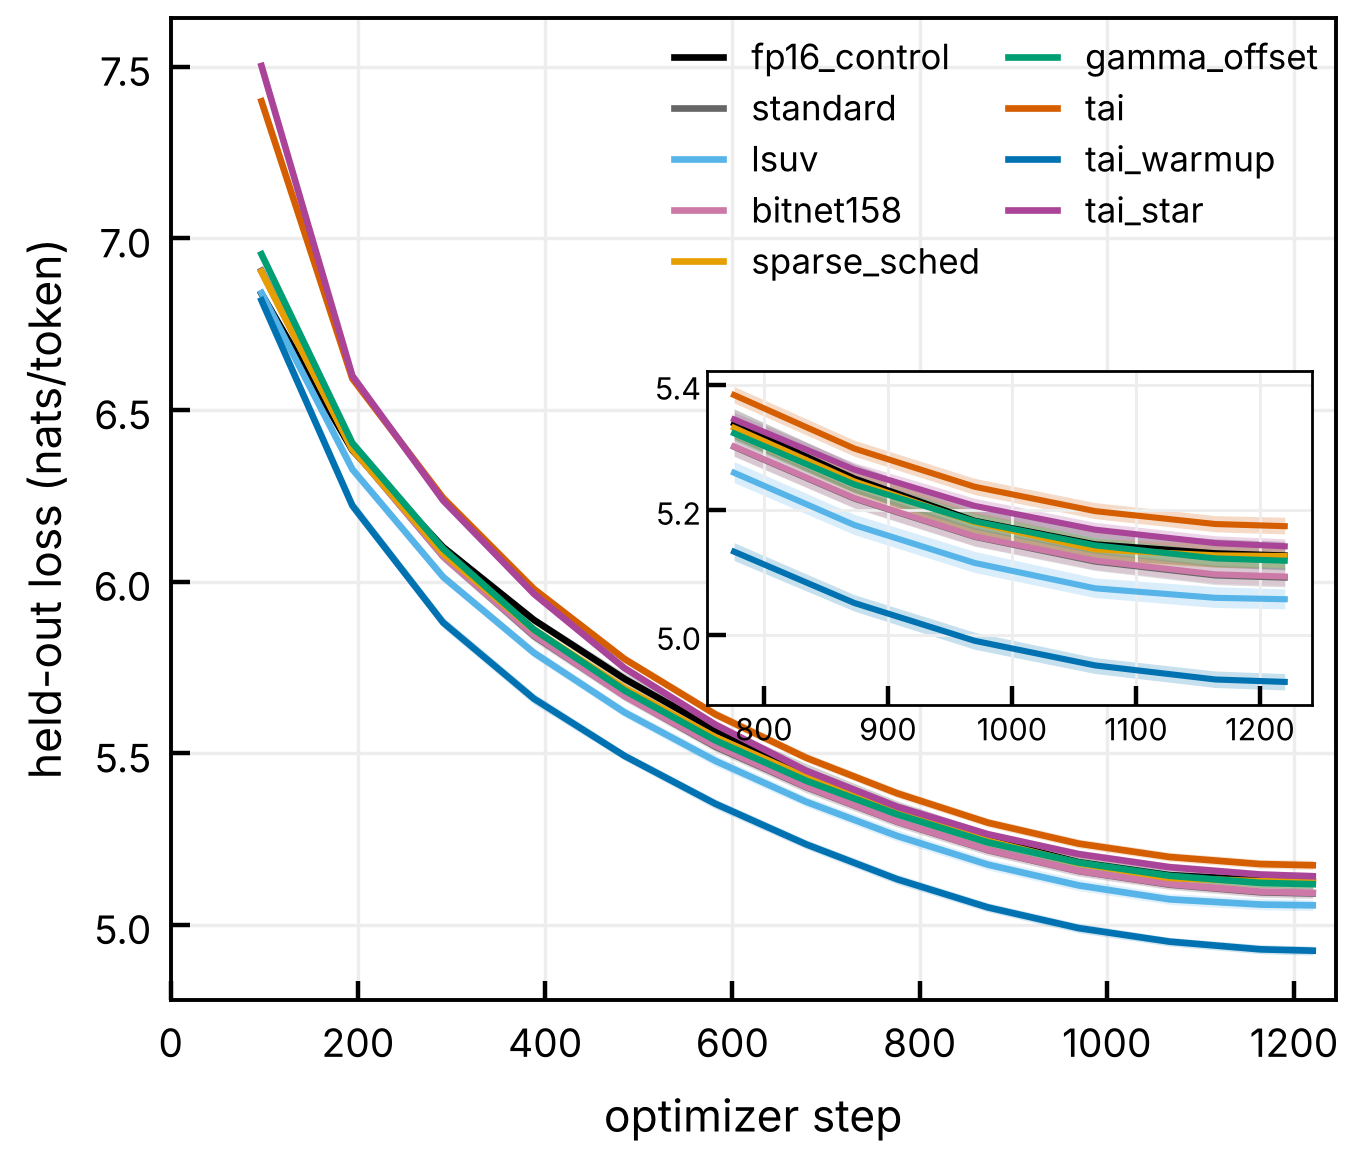
\includegraphics[width=0.86\linewidth]{fig1_convergence.png}
\caption{Held-out loss against optimization step for each arm at the primary
confirmatory scale (\texttt{dim384}), averaged over $15$ seeds at a matched
$20$\,M-token budget. Shaded bands are bootstrap 95\% confidence intervals.}
\label{fig:convergence}
\end{figure}

Table~\ref{tab:primary} reports the complete arm set at the primary
confirmatory scale. Figure~\ref{fig:convergence} shows the corresponding loss
trajectories and Fig.~\ref{fig:finalloss} the paired contrast against the
pre-registered baseline at every ladder point.

\begin{table}[t]
\centering
\footnotesize
\caption{Complete method set at the primary confirmatory scale
(\texttt{dim384}, $8.26$\,M non-embedding parameters, $n=15$ seeds,
$20$\,M-token budget). $\mathcal{L}$: held-out cross-entropy (nats/token);
CI: half-width of the 95\% confidence interval of the mean
(Student $t$, $n=15$); $s$: standard
deviation across seeds; $\mathrm{sp}_T$: final ternary sparsity;
$S_{\mathrm{target}}$: steps to reach the calibrated target loss of $5.6539$
nats; $a_{\mathrm{nt}}$: next-token top-1 accuracy. The pre-registered primary
baseline is \texttt{bitnet158}.}
\label{tab:primary}
\begin{tabular}{@{}lrrrrrr@{}}
\toprule
Arm & $\mathcal{L}$ & CI & $s$ & $\mathrm{sp}_T$ & $S_{\mathrm{target}}$ & $a_{\mathrm{nt}}$ \\
\midrule
\texttt{fp16\_control} & 5.1785 & 0.0248 & 0.0447 & \phantom{0}0.0\% & 564 & 0.216 \\
\texttt{standard} & 5.1094 & 0.0170 & 0.0307 & 32.1\% & 552 & 0.227 \\
\texttt{lsuv} & 5.0752 & 0.0185 & 0.0334 & 31.8\% & 524 & 0.230 \\
\texttt{bitnet158} & 5.1114 & 0.0161 & 0.0291 & 32.1\% & 555 & 0.227 \\
\texttt{sparse\_sched} & 5.1440 & 0.0205 & 0.0370 & 48.8\% & 564 & 0.224 \\
\texttt{gamma\_offset} & 5.1365 & 0.0143 & 0.0258 & 26.0\% & 560 & 0.224 \\
\texttt{tai} & 5.1914 & 0.0150 & 0.0271 & 30.0\% & 613 & 0.221 \\
\textbf{\texttt{tai\_warmup}} & \textbf{4.9437} & 0.0150 & 0.0272 & 30.3\% & \textbf{448} & \textbf{0.242} \\
\texttt{tai\_star} & 5.1919 & 0.0135 & 0.0244 & 28.4\% & 589 & 0.218 \\
\bottomrule
\end{tabular}
\end{table}

Three orderings organize the results. The first two are reproduced at every
ladder point (Fig.~\ref{fig:finalloss}).

\begin{enumerate}
\renewcommand{\labelenumi}{(\roman{enumi})}
\item \textbf{\texttt{tai\_warmup} attains the lowest loss of any arm.} At the
primary scale it improves on the pre-registered baseline by $0.168$ nats and
on the full-precision control by $0.235$ nats.

\item \textbf{\texttt{tai} attains a higher loss than every locked-$\rhoz$
ternary baseline.} At the primary scale it is $0.080$ nats above
\texttt{bitnet158} and $0.116$ nats above \texttt{lsuv}. The two variants of
the proposed method therefore lie on opposite sides of the baseline, and
\texttt{tai\_star} (Section~\ref{sec:res-h8}) tracks \texttt{tai}.

\item \textbf{The gradual-pruning baseline \texttt{sparse\_sched} is the
weakest ternary baseline at the primary scale} ($5.1440$ nats) while attaining by far the highest sparsity
($48.8\%$), and \texttt{gamma\_offset} at its grid-default $\rhoz = 0.75$ sits
between the locked baselines and \texttt{tai}.
\end{enumerate}

\begin{figure*}[t]
\centering
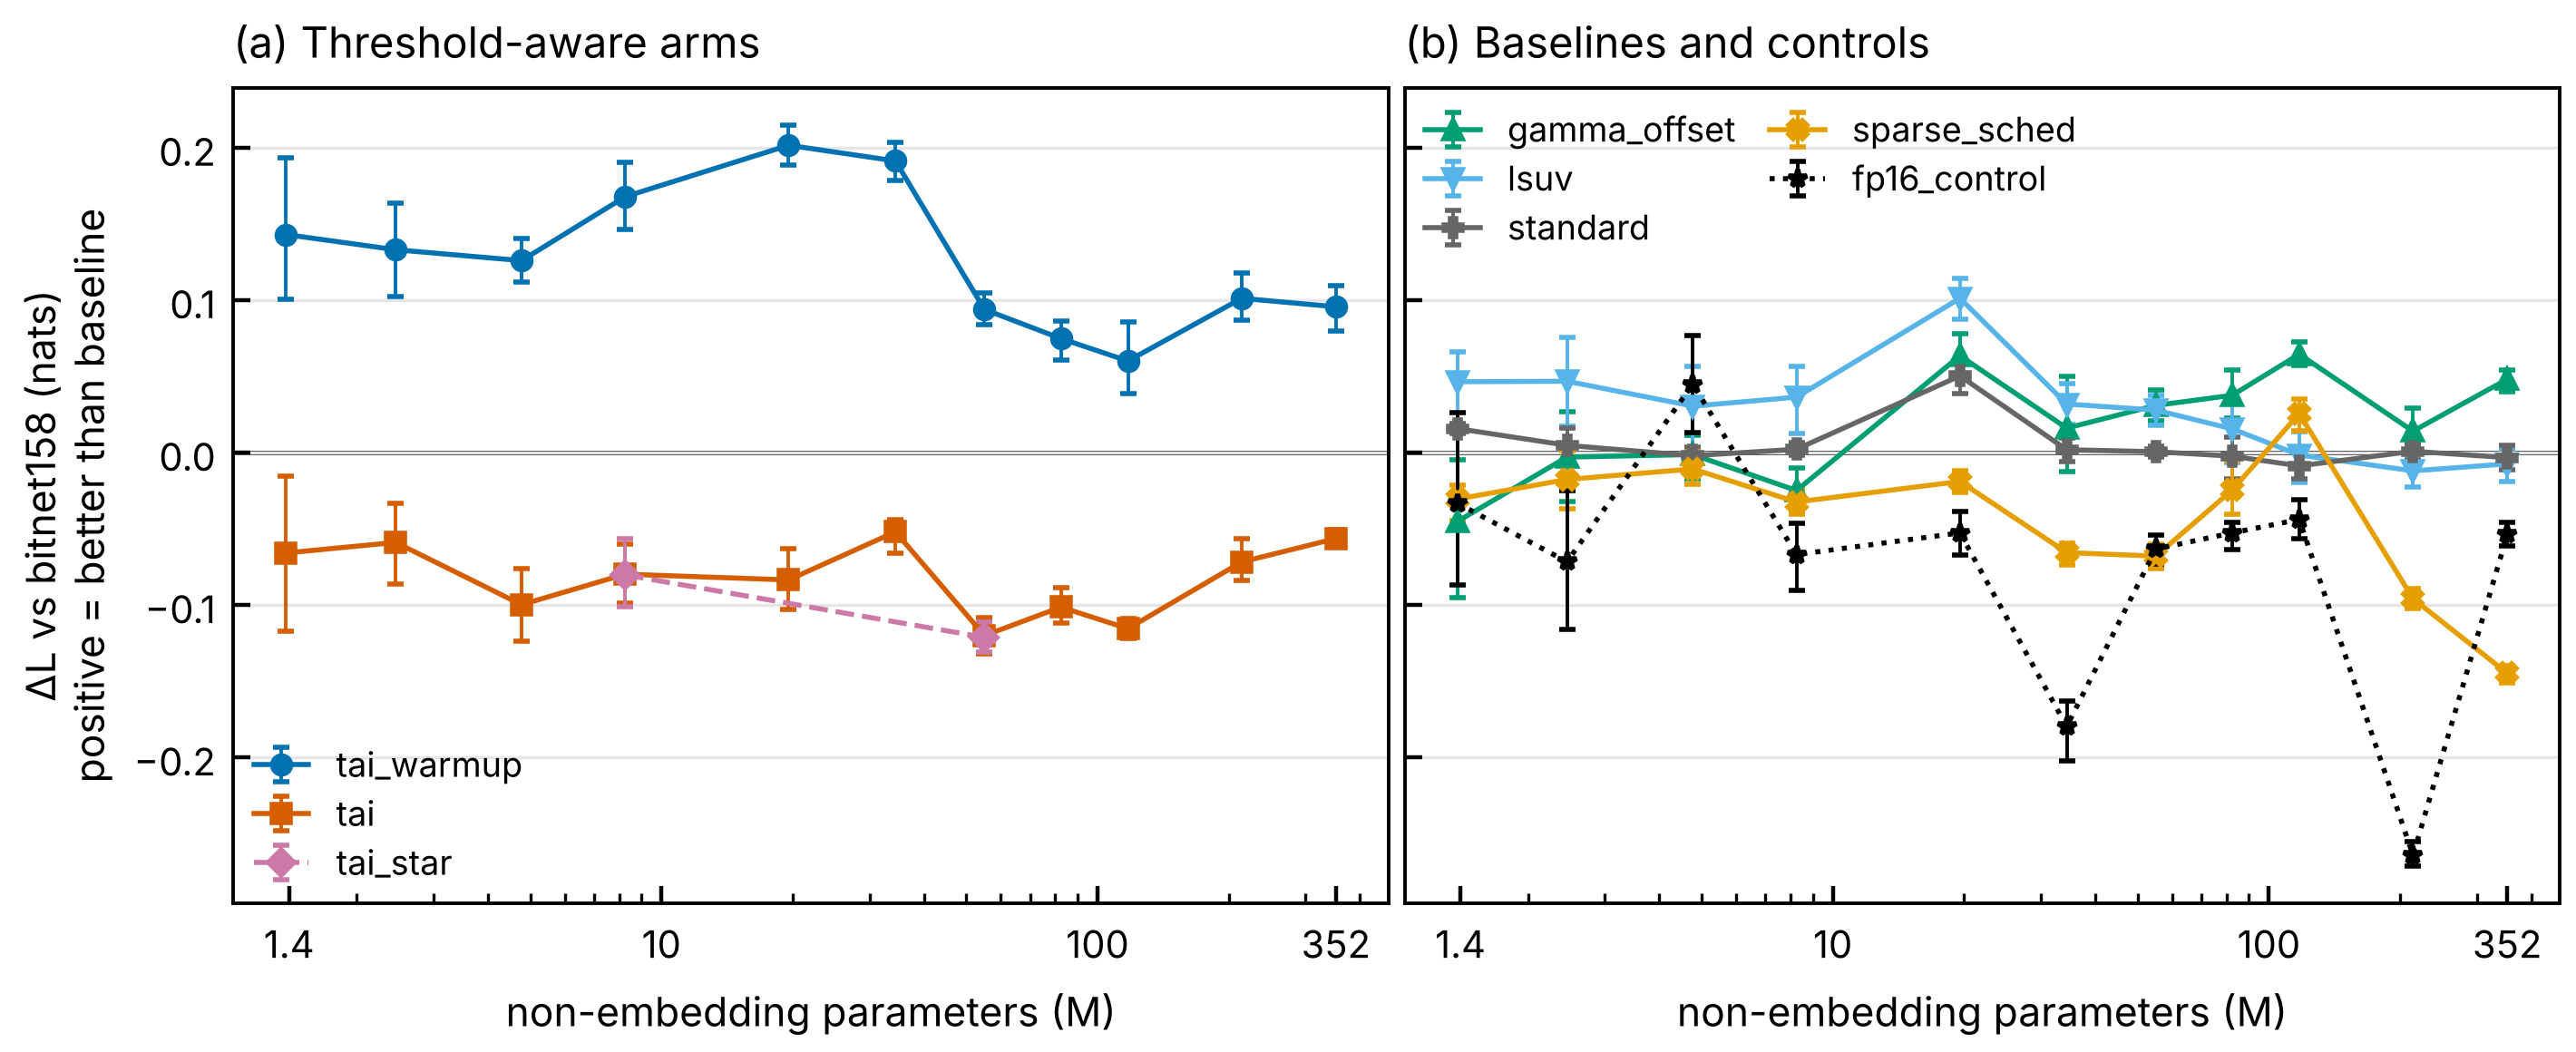
\includegraphics[width=\linewidth]{fig2_final_loss.png}
\caption{Paired quality contrast against the pre-registered baseline across the
eleven-point ladder. Each point is
$\dL = \mathcal{L}(\texttt{bitnet158}) - \mathcal{L}(\mathrm{arm})$, averaged
over the seeds the two arms share at that scale, so positive values favour the
arm; bars are bootstrap 95\% confidence intervals over seeds ($n = 15$ at the
four confirmatory scales, $n = 5$ elsewhere). Panel (a): the threshold-aware
arms, with \texttt{tai\_warmup} above the baseline at every scale and
\texttt{tai} below it at every scale. Panel (b): the remaining baselines and
the full-precision control. \texttt{tai\_star} was executed at \texttt{dim384}
and \texttt{dim768} only. Absolute losses at the primary scale are in
Table~\ref{tab:primary}; the differences are plotted here because they span
$0.26$ nats against absolute losses near $5$.}
\label{fig:finalloss}
\end{figure*}

A result that requires explicit statement is that the ternary arms do not sit
above the full-precision control at this budget. That control is named
\texttt{fp16\_control} after its harness identifier but runs in
\texttt{bfloat16} throughout (Table~\ref{tab:arms}). Taking the strongest non-TAI
ternary arm at each scale, we find that ternary training attains the lower
loss at ten of the eleven ladder points, by between
$0.080$ and $0.278$ nats; the sole exception is \texttt{dim320}, where
\texttt{bitnet158} is $0.045$ nats above \texttt{fp16\_control}. Two properties
of the protocol are recorded alongside this observation without further
interpretation, which is deferred to Section~\ref{sec:discussion}: the
budget does not reach convergence for any arm (Section~\ref{sec:res-budget}),
and the full-precision arm selects a strictly smaller calibrated learning rate
than the ternary arms at five of the eleven scales, though its optimum is
bracketed by the grid at all of them (Section~\ref{sec:res-validity}).

%-----------------------------------------------------------------------------
\subsection{H1: convergence speed at a matched target loss}
\label{sec:res-h1}

Steps-to-target is measured against the calibrated target of $5.6539$ nats,
fixed before the grid on the disjoint calibration seeds. The results are
reported in the $\dS$ column of Table~\ref{tab:crossscale}.

\texttt{tai\_warmup} reaches the target in fewer steps than the primary
baseline at all eleven scales, with $\dS$ ranging from $+28$ steps
(\texttt{dim1280}) to $+148$ steps (\texttt{dim512}). Every statistic in this
subsection is computed on $S_{\mathrm{target}}$ and is therefore distinct from
the held-out-loss columns of Table~\ref{tab:crossscale}: Cohen's $d$ on steps
lies between $+2.39$ and $+7.95$, all eleven paired $t$-tests reject at
$\alpha = 0.05$, and ten of eleven reject at the standalone level
$\alpha_{0} = 0.0125$ fixed in the design, the exception being
\texttt{dim192} ($p = 0.0138$).

\texttt{tai} requires more steps than the baseline at all eleven scales,
with $\dS$ between $-48$ and $-100$ and steps-based $d$ between $-1.52$ and
$-4.47$; ten of eleven contrasts are significant at $\alpha = 0.05$ (\texttt{dim192}:
$p = 0.1248$).

H1 as pre-registered is therefore supported for the schedule variant and
rejected in the opposite direction for the fixed-$\rhoz$ variant.

%-----------------------------------------------------------------------------
\subsection{H2: quality at a fixed token budget}
\label{sec:res-h2}

The pre-registered convergence-conditional test is untestable
(Section~\ref{sec:res-budget}). The token-equal companion test, defined over
all paired seeds against the data-derived margin
$\Delta_{\mathrm{eq}} = 0.10\,|\bar{\mathcal{L}}^{(\beta)} -
\bar{\mathcal{L}}^{(\mathrm{fp16})}|$, is reported in
Table~\ref{tab:crossscale}.

\begin{table*}[t]
\centering
\scriptsize
\caption{Cross-scale paired contrasts against the pre-registered primary
baseline \texttt{bitnet158}. $\dL$ and $\dS$ follow Eq.~\eqref{eq:dL}
(positive favours the method). $\mathrm{CI}_{95}$ is the nonparametric
bootstrap interval on $\dL$ over $5{,}000$ resamples; $d$ is Cohen's $d$;
$p_t$ is the paired $t$-test $p$-value; $p_{\mathrm{Lev}}$ is Levene's test for
H4; $\Delta_{\mathrm{eq}}$ is the data-derived equivalence margin, one value
per scale. The verdict column is the token-equal companion decision. Confirmatory scales are set in
bold. $n$ is the number of paired seeds.}
\label{tab:crossscale}
\begin{tabular}{@{}llrrrrrrrrl@{}}
\toprule
Scale & Arm & $n$ & $\dL$ & $\mathrm{CI}_{95}$ & $d$ & $p_t$ & $\dS$ & $p_{\mathrm{Lev}}$ & $\Delta_{\mathrm{eq}}$ & Verdict \\
\midrule
\texttt{dim192} & \texttt{tai} & 5 & $-0.0661$ & $[-0.117,-0.016]$ & $-1.83$ & 0.0922 & $-88$ & 0.615 & 0.0033 & inconclusive \\
& \texttt{tai\_warmup} & 5 & $+0.1428$ & $[+0.101,+0.191]$ & $+4.33$ & 0.0051 & $+108$ & 0.285 &  & better \\
\textbf{\texttt{dim256}} & \texttt{tai} & 15 & $-0.0591$ & $[-0.086,-0.033]$ & $-1.45$ & 0.0008 & $-63$ & 0.036 & 0.0072 & worse \\
& \texttt{tai\_warmup} & 15 & $+0.1329$ & $[+0.102,+0.164]$ & $+2.88$ & $<10^{-4}$ & $+101$ & 0.447 &  & better \\
\texttt{dim320} & \texttt{tai} & 5 & $-0.1000$ & $[-0.124,-0.076]$ & $-4.79$ & 0.0021 & $-100$ & 0.996 & 0.0045 & worse \\
& \texttt{tai\_warmup} & 5 & $+0.1257$ & $[+0.111,+0.140]$ & $+5.31$ & 0.0001 & $+92$ & 0.707 &  & better \\
\textbf{\texttt{dim384}} & \texttt{tai} & 15 & $-0.0800$ & $[-0.099,-0.060]$ & $-2.84$ & $<10^{-4}$ & $-59$ & 0.648 & 0.0067 & worse \\
& \texttt{tai\_warmup} & 15 & $+0.1677$ & $[+0.146,+0.190]$ & $+5.95$ & $<10^{-4}$ & $+107$ & 0.889 &  & better \\
& \texttt{tai\_star} & 15 & $-0.0805$ & $[-0.102,-0.057]$ & $-3.00$ & $<10^{-4}$ & $-35$ & 0.532 &  & worse \\
\textbf{\texttt{dim512}} & \texttt{tai} & 15 & $-0.0838$ & $[-0.104,-0.064]$ & $-3.59$ & $<10^{-4}$ & $-71$ & 0.175 & 0.0053 & worse \\
& \texttt{tai\_warmup} & 15 & $+0.2014$ & $[+0.188,+0.214]$ & $+11.26$ & $<10^{-4}$ & $+148$ & 0.347 &  & better \\
\texttt{dim640} & \texttt{tai} & 5 & $-0.0522$ & $[-0.066,-0.044]$ & $-5.12$ & 0.0016 & $-48$ & 0.871 & 0.0180 & worse \\
& \texttt{tai\_warmup} & 5 & $+0.1911$ & $[+0.178,+0.204]$ & $+13.01$ & $<10^{-4}$ & $+104$ & 0.633 &  & better \\
\textbf{\texttt{dim768}} & \texttt{tai} & 15 & $-0.1203$ & $[-0.132,-0.109]$ & $-6.35$ & $<10^{-4}$ & $-95$ & 0.957 & 0.0063 & worse \\
& \texttt{tai\_warmup} & 15 & $+0.0937$ & $[+0.084,+0.105]$ & $+5.32$ & $<10^{-4}$ & $+53$ & 0.593 &  & better \\
& \texttt{tai\_star} & 15 & $-0.1214$ & $[-0.131,-0.111]$ & $-7.23$ & $<10^{-4}$ & $-95$ & 0.461 &  & worse \\
\texttt{dim896} & \texttt{tai} & 5 & $-0.1016$ & $[-0.112,-0.091]$ & $-6.63$ & 0.0001 & $-72$ & 0.360 & 0.0053 & worse \\
& \texttt{tai\_warmup} & 5 & $+0.0746$ & $[+0.061,+0.086]$ & $+6.38$ & 0.0006 & $+40$ & 0.819 &  & better \\
\texttt{dim1024} & \texttt{tai} & 5 & $-0.1157$ & $[-0.122,-0.109]$ & $-12.12$ & $<10^{-4}$ & $-100$ & 0.334 & 0.0044 & worse \\
& \texttt{tai\_warmup} & 5 & $+0.0599$ & $[+0.039,+0.085]$ & $+3.48$ & 0.0102 & $+32$ & 0.621 &  & better \\
\texttt{dim1280} & \texttt{tai} & 5 & $-0.0720$ & $[-0.084,-0.057]$ & $-5.75$ & 0.0008 & $-72$ & 0.389 & 0.0264 & worse \\
& \texttt{tai\_warmup} & 5 & $+0.1010$ & $[+0.087,+0.116]$ & $+8.99$ & 0.0003 & $+28$ & 0.163 &  & better \\
\texttt{dim1536} & \texttt{tai} & 5 & $-0.0566$ & $[-0.062,-0.051]$ & $-5.81$ & 0.0001 & $-68$ & 0.385 & 0.0054 & worse \\
& \texttt{tai\_warmup} & 5 & $+0.0954$ & $[+0.079,+0.110]$ & $+8.27$ & 0.0004 & $+36$ & 0.955 &  & better \\
\bottomrule
\end{tabular}
\end{table*}

The bootstrap interval excludes zero in all $24$ cells, so the sign of $\dL$
is resolved throughout. The one cell whose paired $t$-test does not reach
$\alpha = 0.05$ is \texttt{tai} at \texttt{dim192} ($n=5$, $p_t = 0.0922$),
which is why its verdict is inconclusive. The companion test never returns equivalence: $\Delta_{\mathrm{eq}}$
ranges from $0.0033$ to $0.0264$ nats while $|\dL|$ ranges from $0.052$ to
$0.201$ nats, i.e.\ every observed difference exceeds its margin by between
$2.7\times$ and $42.9\times$. The verdicts are accordingly categorical:
\texttt{tai\_warmup} is superior to the baseline at all eleven scales;
\texttt{tai} is inferior at ten of eleven and inconclusive at the eleventh.

Holm--Bonferroni correction within the confirmatory held-out-loss family, at
family-wise level $\alpha_{H} = 0.05$, rejects the null for both TAI variants
at every scale except \texttt{tai} at \texttt{dim192}, which is retained. The Wilcoxon signed-rank test, computed
wherever $n \geq 6$, supports the parametric verdict in every case
($p \leq 0.0009$).

The secondary sensitivity contrast against the data-selected minimum baseline
attenuates the \texttt{tai\_warmup} advantage, for
example at \texttt{dim512}, $\dL$ falls from $+0.201$ (versus
\texttt{bitnet158}) to $+0.100$ (versus \texttt{lsuv}), and at \texttt{dim768}
from $+0.094$ to $+0.063$ (versus \texttt{gamma\_offset}). The sign survives at
ten of the eleven scales and reverses at \texttt{dim1024}, where
\texttt{gamma\_offset} is the strongest baseline and $\dL = -0.0044$. This contrast is
exploratory and carries no family-wise correction.

%-----------------------------------------------------------------------------
\subsection{H4: outcome variance}
\label{sec:res-h4}

Levene's test finds no evidence that either TAI variant inflates variance
relative to the baseline. Across the $24$ cells of Table~\ref{tab:crossscale},
$p_{\mathrm{Lev}}$ falls below $0.05$ in exactly one
(\texttt{dim256}/\texttt{tai}, $p = 0.036$). That cell does not bear on H4 in
the direction the hypothesis concerns: the TAI standard deviation there is
less than half the baseline's ($0.0237$ versus $0.0525$), so what the test
detects is a reduction in spread, not inflation. It also does not survive the
pre-registered per-hypothesis level $\alpha_{0} = 0.0125$.

The pre-registered form of H4 is evaluated on the pooled seed $\times$ fold
matrix, in which every trained model is scored on all $K=5$ held-out sub-folds.
Table~\ref{tab:h4} reports the decomposition at the primary scale.

\begin{table}[t]
\centering
\small
\caption{Variance decomposition for H4 at the primary scale
(\texttt{dim384}, $15$ seeds $\times$ $5$ held-out folds). Mean $\mathcal{L}$
is the grand mean over all five folds and therefore differs from the fold-$0$
value of Table~\ref{tab:primary}. Levene's test on the
pooled matrix is the pre-registered statistic.}
\label{tab:h4}
\begin{tabular}{@{}lrrrr@{}}
\toprule
Arm & Mean $\mathcal{L}$ & $s$ across seeds & $s$ across folds & $s$ pooled \\
\midrule
\texttt{tai} & 5.2113 & 0.0272 & 0.0328 & 0.0397 \\
\texttt{bitnet158} & 5.1324 & 0.0309 & 0.0339 & 0.0429 \\
\midrule
\multicolumn{5}{@{}l}{Levene, pooled seed $\times$ fold: $W = 0.554$, $p = 0.458$} \\
\multicolumn{5}{@{}l}{Levene, seed only: $W = 0.343$, $p = 0.563$} \\
\bottomrule
\end{tabular}
\end{table}

H4 is supported: there is no evidence of variance inflation
($p = 0.458$, clearing both the conventional $0.05$ and the pre-registered
$\alpha_{0} = 0.0125$), and this holds whether or not data-sampling
spread is included. A secondary observation from the decomposition is that the
dominant variance component is the evaluation fold rather than the seed
(mean $s$ across folds $0.0334$ versus across seeds $0.0290$), for both arms.

%-----------------------------------------------------------------------------
\subsection{H3: control of the ternary operating point and its retention}
\label{sec:res-h3}

\begin{figure}[t]
\centering
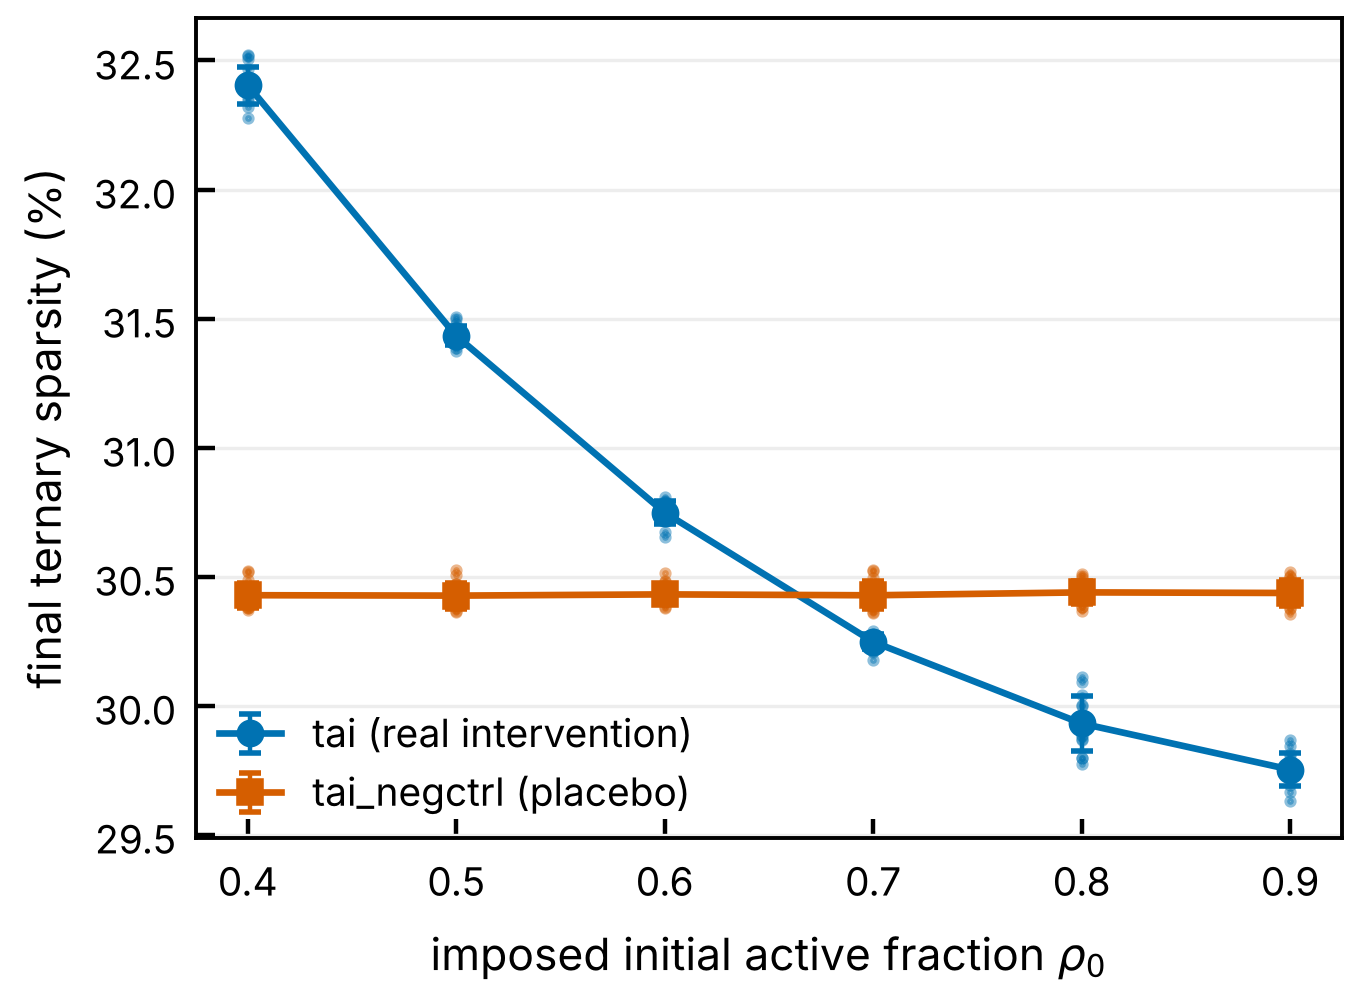
\includegraphics[width=0.86\linewidth]{fig3_rho0_sweep.png}
\caption{Final ternary sparsity, in per cent, as a function of the imposed
initial active fraction $\rhoz$ at the primary scale (\texttt{dim384}), for
the \texttt{tai} arm and for the $\rhoz$-labelled placebo
\texttt{tai\_negctrl}. Every one of the $15$ seeds per point is shown, with
the mean and one standard deviation. The placebo
holds the realized threshold partition fixed at $\rhoz = 0.69$ while varying
only the label, so any dependence it exhibits is measurement artefact.}
\label{fig:sweep}
\end{figure}

\subsubsection{Ordinal control}

The rank association between $\rhoz$ and final sparsity is essentially perfect
and negative, as predicted (Fig.~\ref{fig:sweep}): a larger initial active
fraction implies fewer terminal zeros. At the primary scale the pooled Spearman coefficient is
$-0.983$ ($p = 4.3\times 10^{-66}$) and the mean per-seed coefficient is
$-0.996$, 95\% CI $[-1.000, -0.989]$ over $15$ seeds, with $93\%$ of seeds
strictly monotone. The intervention is far above the nuisance floor: the
across-$\rhoz$ range of final sparsity is $0.0265$ against a within-$\rhoz$
across-seed standard deviation of $0.00059$, a signal-to-noise ratio of
$44.9\times$. The control is statistically indistinguishable across scale
(\texttt{dim384} mean $-0.996 \pm 0.015$ versus \texttt{dim768}
$-1.000 \pm 0.000$; Welch $t = +1.00$, $p = 0.334$).

\subsubsection{Retention: how much of the intervention survives training}

The ordinal result establishes that the ordering survives; it does not
establish that the magnitude does. Regressing final on initial sparsity
per Eq.~\eqref{eq:retention} gives the retention coefficients of
Table~\ref{tab:retention}, which is the principal quantitative result of this
section.

\begin{table*}[t]
\centering
\small
\caption{Retention of the operating-point intervention,
$\mathrm{sp}_T = \mathrm{sp}_\infty + r\,\mathrm{sp}_0$, over the six-point
$\rhoz$ grid at $15$ seeds per point. A $50$-percentage-point swing in initial
sparsity is imposed in every cell. $r$: retention coefficient; final swing: the
resulting range of final sparsity.}
\label{tab:retention}
\begin{tabular}{@{}llrrrr@{}}
\toprule
Scale & Arm & $r$ & $R^{2}$ & Final swing & Implied fixed point \\
\midrule
\texttt{dim384} & \texttt{tai} & 0.052 & 0.931 & \phantom{0}2.65 pt & 0.305 \\
\texttt{dim384} & \texttt{gamma\_offset} & 1.003 & 1.000 & 50.09 pt & n/a \\
\texttt{dim768} & \texttt{tai} & 0.069 & 0.959 & \phantom{0}3.55 pt & 0.300 \\
\texttt{dim768} & \texttt{gamma\_offset} & 1.006 & 1.000 & 50.33 pt & n/a \\
\bottomrule
\end{tabular}
\end{table*}

The two mechanisms behave qualitatively differently. For the TAI arm, a
$50$-point swing in initial sparsity produces a final swing of $2.65$ points at
\texttt{dim384} and $3.55$ points at \texttt{dim768}: retention is
$0.052$--$0.069$, so approximately $93$--$95\%$ of the imposed intervention is
erased during training. The residual is nonetheless perfectly ordered and
highly reproducible, the within-cell standard deviation being $3$--$11\times
10^{-4}$. The implied fixed point is $0.305$ at \texttt{dim384} and $0.300$ at
\texttt{dim768}; for reference, the \texttt{standard} arm reaches $0.321$ and
$0.318$ at those scales without any intervention.

For the $\gamma$-offset arm, retention is $1.003$ and $1.006$ with
$R^{2} = 1.000$ at both scales: the final operating point tracks the target
one-for-one across the entire $50$-point range
(Table~\ref{tab:sweep}). This arm reaches its operating point by holding the
threshold scale at the constant $c^{\star}(\rhoz)$ of Eq.~\eqref{eq:cstar},
whose calibrated values over the grid are $2.110$, $1.691$, $1.314$, $0.966$,
$0.635$ and $0.315$ for $\rhoz = 0.4,\dots,0.9$.

H3 as pre-registered, that the initial operating point causally shapes the
final learned sparsity, is therefore \textbf{not supported in its strong form
for the initialization mechanism}, and is supported almost exactly for the
threshold-offset mechanism. The operative statement for the initialization
variant is a bounded residual effect with the retention fraction reported.

\subsubsection{Pre-registered falsification}

\begin{figure*}[t]
\centering
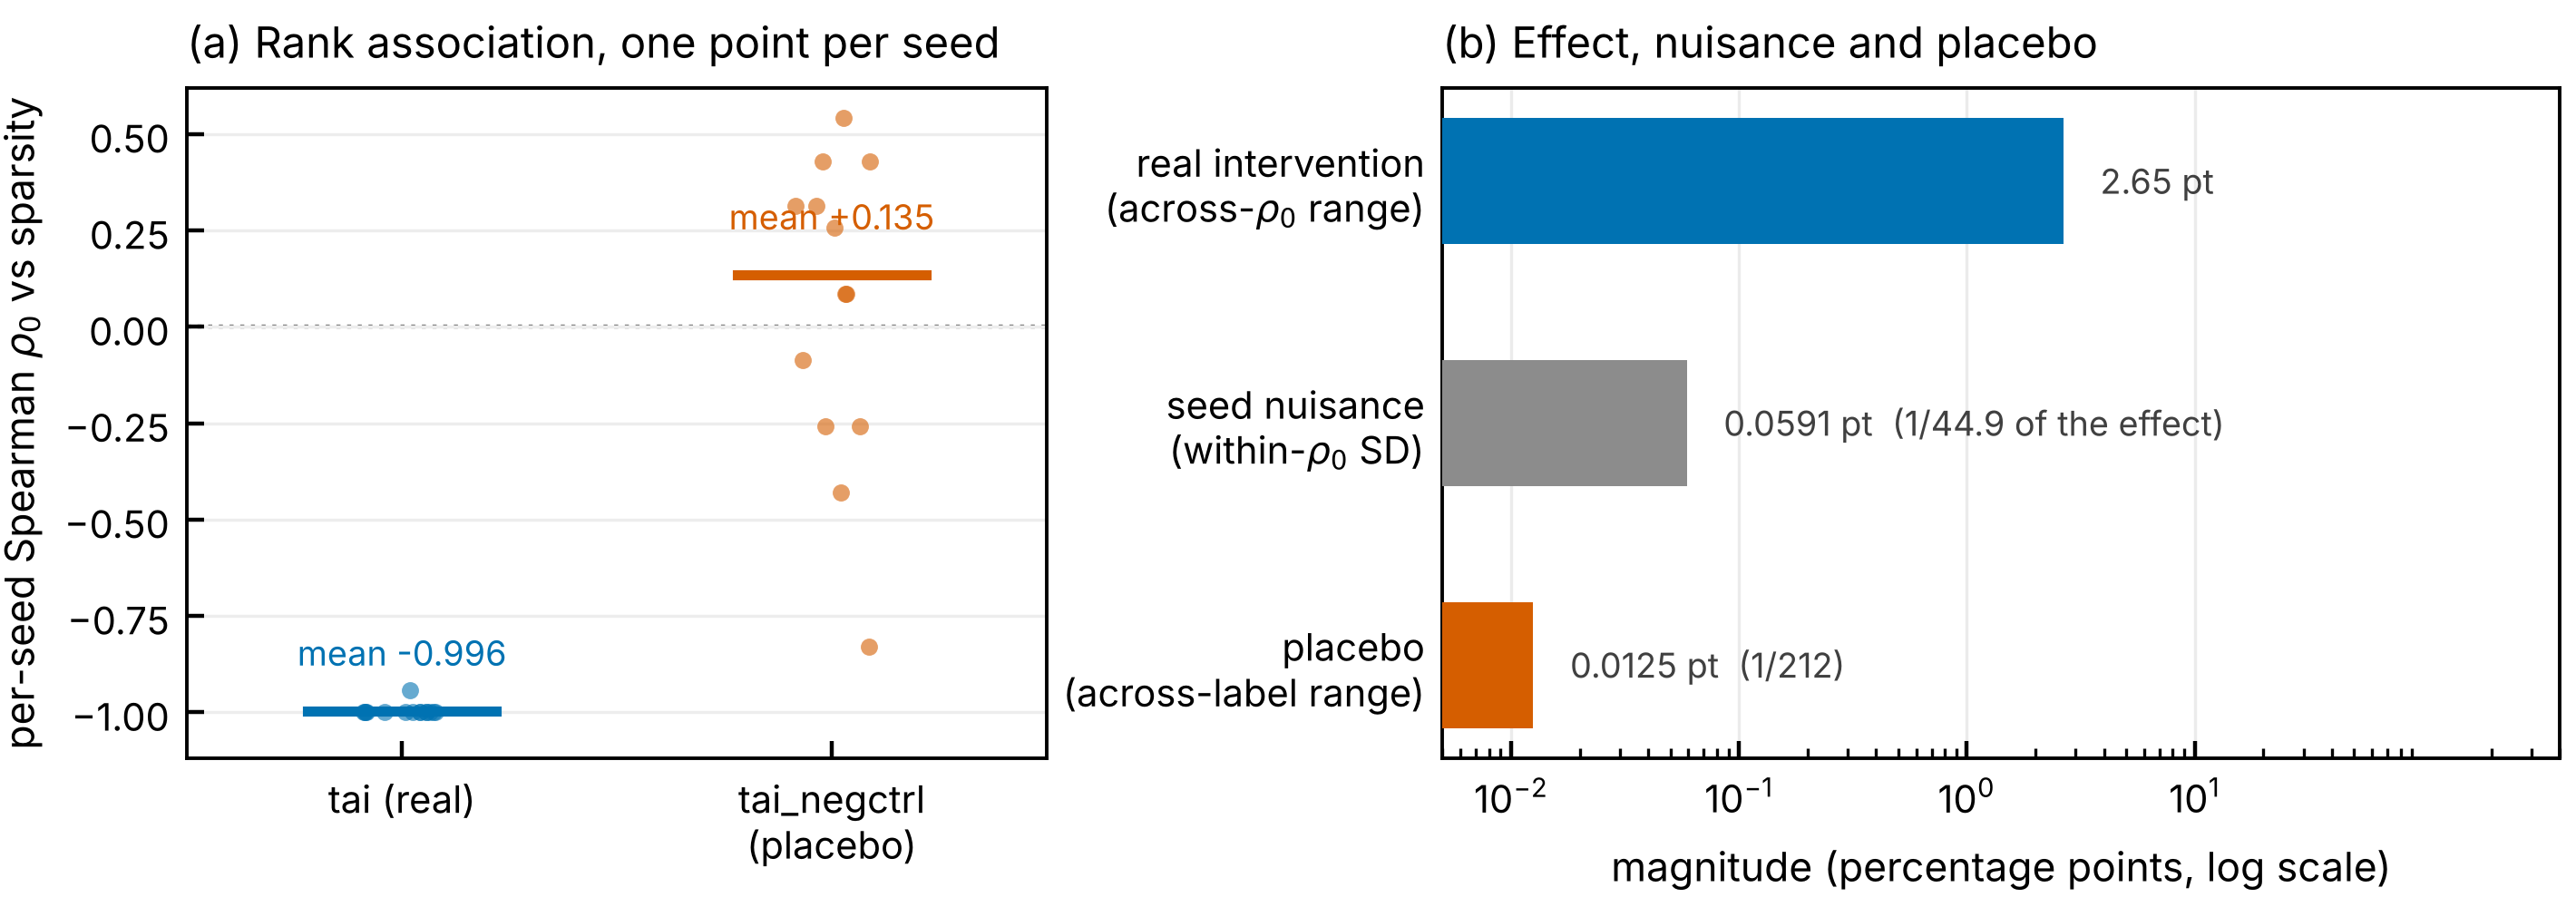
\includegraphics[width=\linewidth]{fig7_h3_falsification.png}
\caption{Pre-registered falsification instrument for H3; the sweep itself is
Fig.~\ref{fig:sweep}. Panel (a): the per-seed Spearman coefficient between the
imposed $\rhoz$ label and final sparsity, one point per seed, for the real
intervention and for the placebo \texttt{tai\_negctrl}. Panel (b): the
across-$\rhoz$ effect, the within-$\rhoz$ seed nuisance and the placebo's
across-label range on one logarithmic axis, so that both ratios quoted in the
text are legible at once. The signed sign test of the pre-registration
($0$ of $15$, $p = 6.1\times10^{-5}$) is not plotted, for the reason given in
the text.}
\label{fig:falsification}
\end{figure*}

The placebo arm \texttt{tai\_negctrl}, which varies the $\rhoz$ label while
holding the realized partition fixed at $0.69$ (Fig.~\ref{fig:falsification}),
produces a final sparsity of $0.3043$--$0.3044$
across all six labels ($n = 15$ per label): a range of
$1.3\times 10^{-4}$, against $2.65\times 10^{-2}$ for the real intervention, a
factor of $212$. The placebo's mean per-seed Spearman coefficient is $+0.135$,
generated entirely by fourth-decimal noise and of opposite sign to the real
effect ($-0.996$). The pre-registered sign test records the real coefficient as
exceeding the placebo coefficient in $0$ of $15$ seeds
($p = 6.1\times 10^{-5}$); because the test was specified as a one-sided
comparison of signed coefficients while the true effect is negative, this
statistic is reported here for completeness and the magnitude comparison above
is the interpretable falsification result. The placebo is flat, as predicted,
and the sparsity effect is therefore not an artefact of the analysis.

%-----------------------------------------------------------------------------
\subsection{H5: the quality-sparsity frontier}
\label{sec:res-h5}

\begin{figure*}[t]
\centering
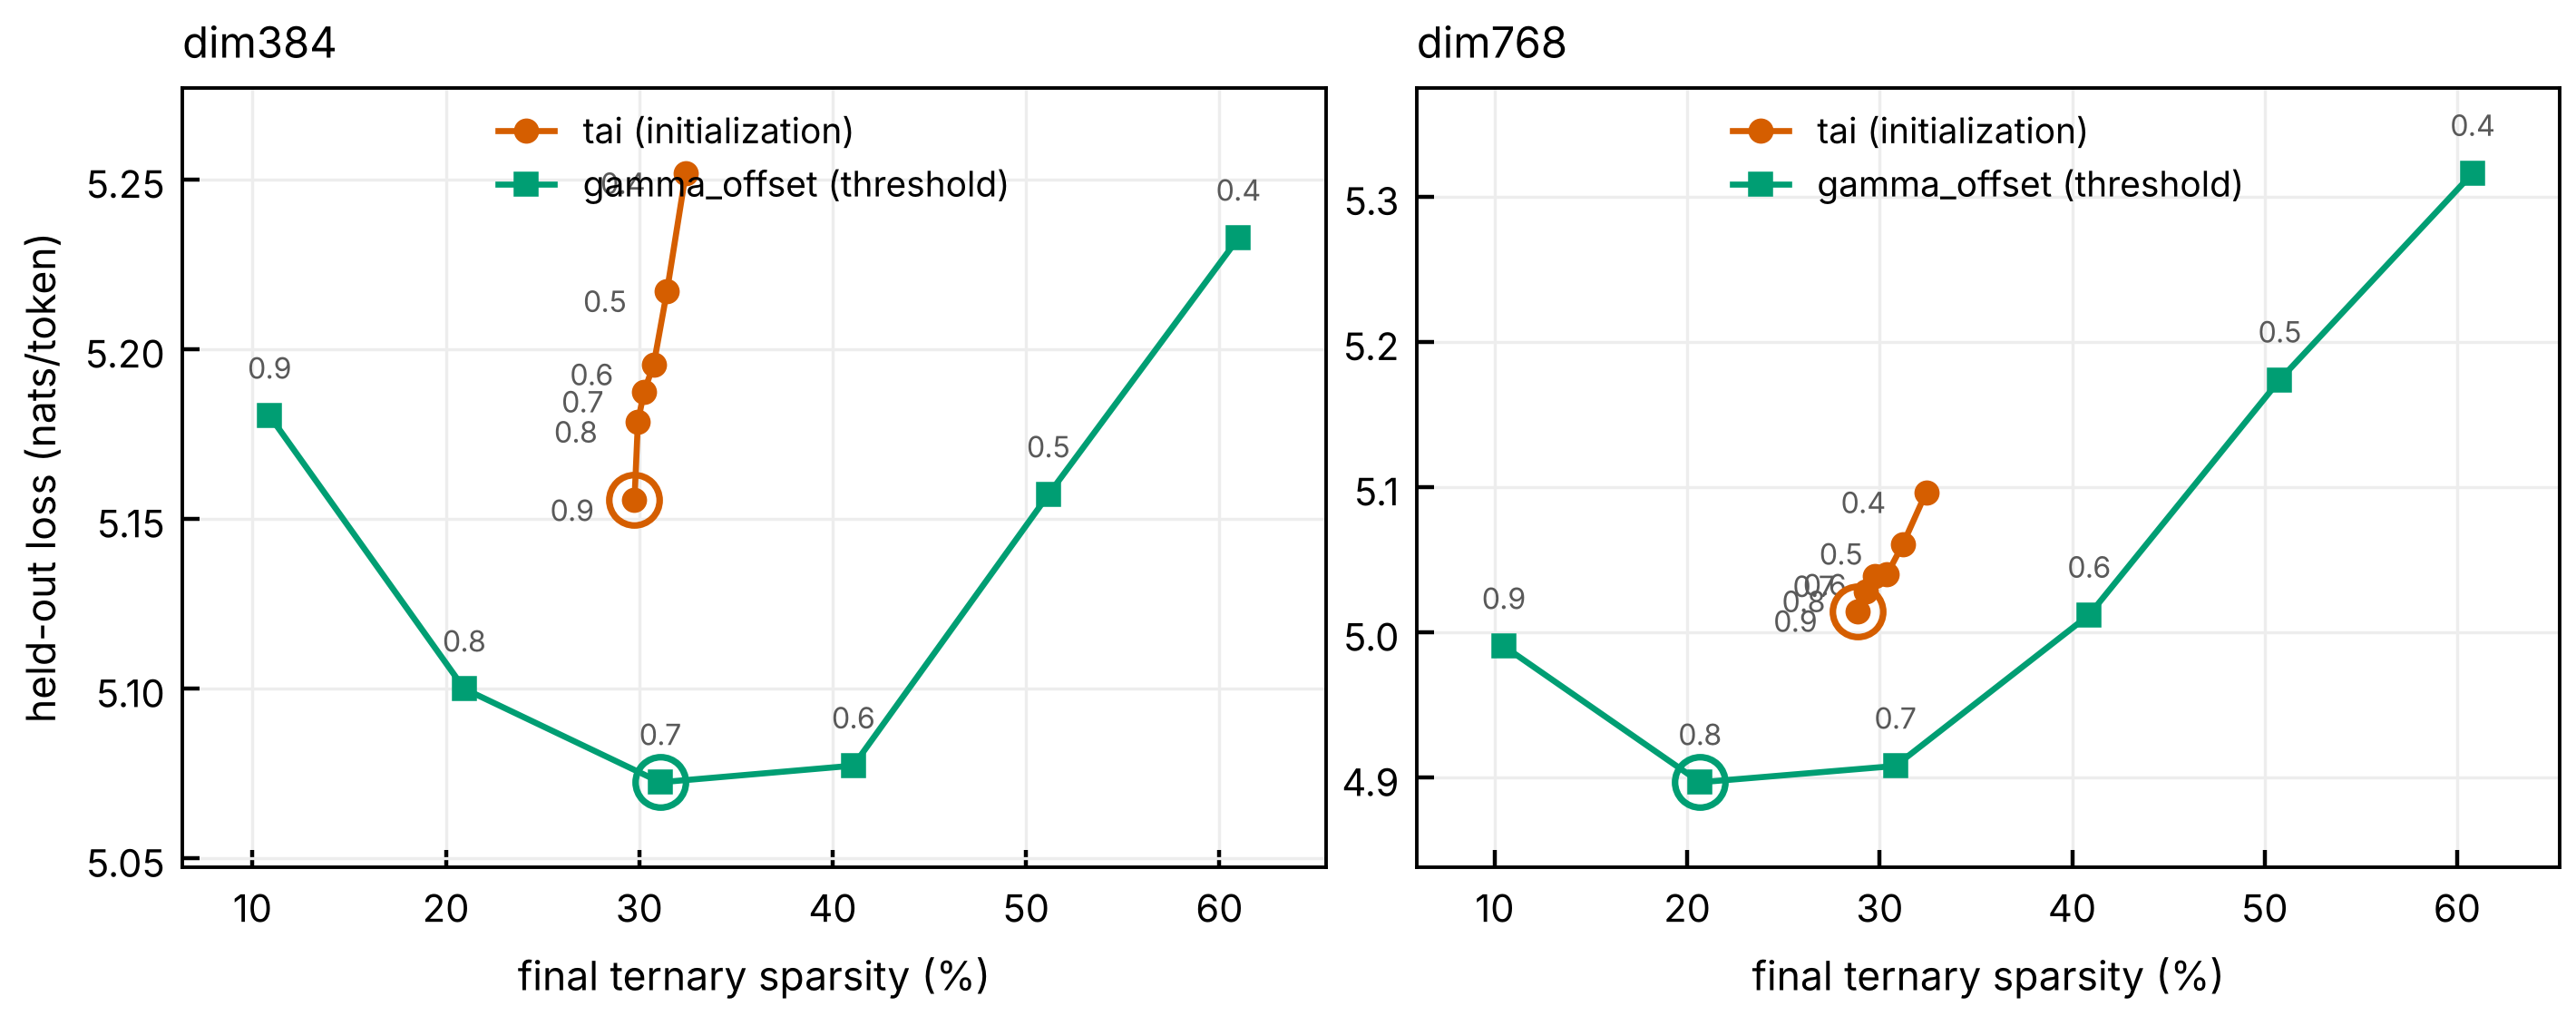
\includegraphics[width=\linewidth]{fig5_pareto.png}
\caption{Held-out loss, in nats per token, against final ternary sparsity, in
per cent, across the $\rhoz$ sweep, for both mechanisms and at both swept
scales. Each point is one operating point, labelled with its $\rhoz$ and
averaged over $15$ seeds; the ringed marker is
each arm's minimum. The threshold-offset arm traces a U-shaped frontier
spanning $50$ points of sparsity with an interior optimum, while the
initialization arm's sparsity axis spans under four points, rendering its
frontier near-degenerate.}
\label{fig:pareto}
\end{figure*}

Table~\ref{tab:sweep} reports the full sweep for both arms at both scales.

\begin{table*}[t]
\centering
\small
\caption{Operating-point sweep. Held-out loss (mean $\pm$ SD over $15$ seeds)
and final ternary sparsity for the initialization mechanism (\texttt{tai}) and
the threshold-offset mechanism (\texttt{gamma\_offset}) at two scales. The
minimum-loss point of each column is set in bold.}
\label{tab:sweep}
\begin{tabular}{@{}crrrrrrrr@{}}
\toprule
& \multicolumn{4}{c}{\texttt{dim384}} & \multicolumn{4}{c}{\texttt{dim768}} \\
\cmidrule(lr){2-5}\cmidrule(lr){6-9}
& \multicolumn{2}{c}{\texttt{tai}} & \multicolumn{2}{c}{\texttt{gamma\_offset}}
& \multicolumn{2}{c}{\texttt{tai}} & \multicolumn{2}{c}{\texttt{gamma\_offset}} \\
$\rhoz$ & $\mathcal{L}$ & $\mathrm{sp}_T$ & $\mathcal{L}$ & $\mathrm{sp}_T$
& $\mathcal{L}$ & $\mathrm{sp}_T$ & $\mathcal{L}$ & $\mathrm{sp}_T$ \\
\midrule
0.4 & 5.2519 & 32.4\% & 5.2328 & 61.0\% & 5.0963 & 32.4\% & 5.3160 & 60.8\% \\
0.5 & 5.2171 & 31.4\% & 5.1572 & 51.2\% & 5.0609 & 31.2\% & 5.1739 & 50.8\% \\
0.6 & 5.1955 & 30.7\% & 5.0774 & 41.1\% & 5.0397 & 30.4\% & 5.0120 & 40.9\% \\
0.7 & 5.1875 & 30.2\% & \textbf{5.0724} & 31.1\% & 5.0386 & 29.8\% & 4.9080 & 30.8\% \\
0.8 & 5.1786 & 29.9\% & 5.1000 & 21.0\% & 5.0282 & 29.3\% & \textbf{4.8968} & 20.7\% \\
0.9 & \textbf{5.1555} & 29.8\% & 5.1804 & 10.9\% & \textbf{5.0146} & 28.9\% & 4.9905 & 10.5\% \\
\bottomrule
\end{tabular}
\end{table*}

For the initialization mechanism the loss decreases monotonically in $\rhoz$
over the whole grid, from $5.2519$ at $\rhoz = 0.4$ to $5.1555$ at
$\rhoz = 0.9$ (\texttt{dim384}), while final sparsity varies by only $2.6$
points; the frontier is consequently near-degenerate, and all six points are
formally non-dominated only because the sparsity differences, though tiny, are
strictly ordered. Under the pre-registered selection rule, minimum loss
subject to $\mathrm{sp}_T \geq 30\%$, the optimum is
$\rhoz^\star = 0.70$ ($\mathcal{L} = 5.1875$, $\mathrm{sp}_T = 30.2\%$), with
bootstrap selection probabilities $P(0.60) = 0.237$, $P(0.70) = 0.758$ and
$\leq 0.003$ elsewhere.

For the threshold-offset mechanism the loss is U-shaped with an interior
optimum, and the sparsity axis spans $50$ points (Fig.~\ref{fig:pareto}). At \texttt{dim384} the
minimum is at $\rhoz = 0.70$ ($\mathcal{L} = 5.0724$ at $31.1\%$ sparsity); at
\texttt{dim768} it is at $\rhoz = 0.80$ ($\mathcal{L} = 4.8968$ at $20.7\%$
sparsity), where the loss is $0.011$ nats below the same arm's $\rhoz = 0.70$
point and $0.020$ nats below the \texttt{dim768} \texttt{bitnet158} baseline
($4.9167$) at two-thirds of its sparsity.

One point associated with this arm does not lie on the curve its neighbours
describe, and is recorded here. The main grid runs \texttt{gamma\_offset} at
the default $\rhoz = 0.75$, which the sweep grid does not contain; at
\texttt{dim384} that point attains $5.1365$, above both $\rhoz = 0.70$
($5.0724$) and $\rhoz = 0.80$ ($5.1000$), by some five standard errors of the
$15$-seed mean. It is not a configuration error: the realized sparsity
interpolates its two neighbours to within $10^{-4}$, and the calibrated
learning rate and the threshold constant $c^{\star}(0.75)$ are the values the
protocol specifies. The sweep and the main grid do, however, fall on opposite
sides of the execution-path split of Section~\ref{sec:res-validity}. We record
the discrepancy rather than resolve it. Contrasts drawn within a single phase
are unaffected, including the main-grid comparison of this arm against the
baseline in Section~\ref{sec:res-gammadefault}; what the discrepancy rules out
is treating the sweep and the main grid as interchangeable measurements of the
same arm.

H5 is therefore supported for the
threshold-offset mechanism, which traces a genuine frontier, and is
uninformative for the initialization mechanism, whose sparsity axis is
effectively fixed.

%-----------------------------------------------------------------------------
\subsection{Mechanism attribution}
\label{sec:res-mechanism}

\begin{figure*}[t]
\centering
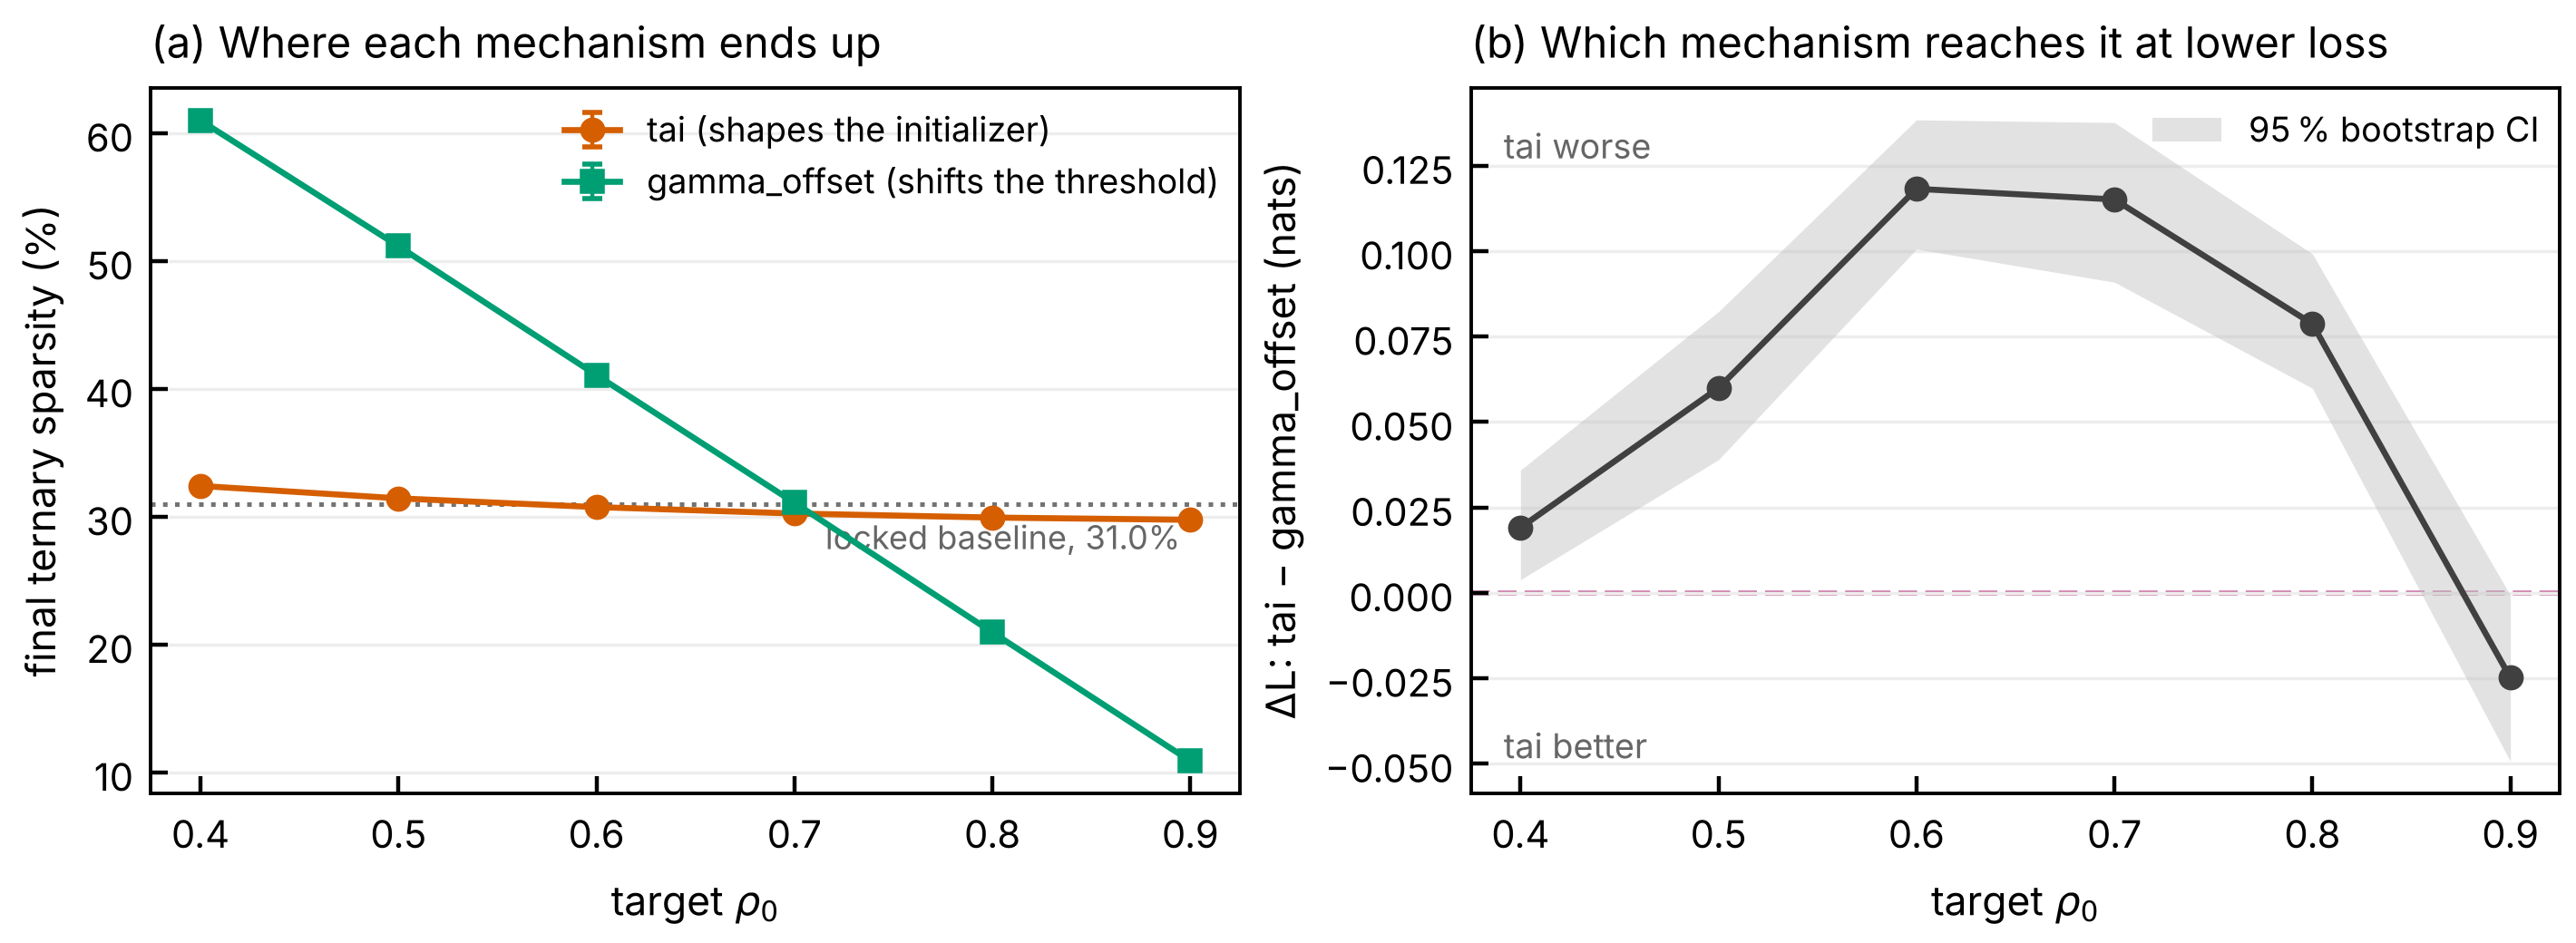
\includegraphics[width=\linewidth]{fig10_mechanism.png}
\caption{Panel (a): the \emph{final} operating point each mechanism reaches as
a function of the target $\rhoz$, with the analytically locked sparsity of
Proposition~\ref{prop:locked} marked. Panel (b): the paired difference in
held-out loss, in nats per token, between the initialization and
threshold-offset mechanisms at matched $\rhoz$, with a bootstrap 95\%
confidence interval over the $15$ seeds; an
interval covering zero would indicate that the two are matched.}
\label{fig:mechanism}
\end{figure*}

\subsubsection{Initialization versus threshold offset}

Paired over all $90$ $(\rhoz, \mathrm{seed})$ cells at the primary scale, the
initialization mechanism attains a loss $0.0610$ nats higher than the
threshold-offset mechanism, 95\% CI $[+0.0474, +0.0742]$, paired
$t$-test $p = 1.06\times 10^{-13}$ (Fig.~\ref{fig:mechanism}). Both arms control the operating point
ordinally with essentially equal reliability (mean per-seed Spearman $-1.000$
for \texttt{gamma\_offset}, $-0.996$ for \texttt{tai}), but only the
threshold-offset arm retains the magnitude (Table~\ref{tab:retention}). Of the
three pre-registered readings of this contrast
(Section~\ref{sec:gammaoffset}), the outcome is the third: the simpler
mechanism wins, on both quality and retention. This contrast is exploratory
and carries no family-wise correction.

\subsubsection{The $2\times 2$ initialization $\times$ precision ablation}

\begin{figure}[t]
\centering
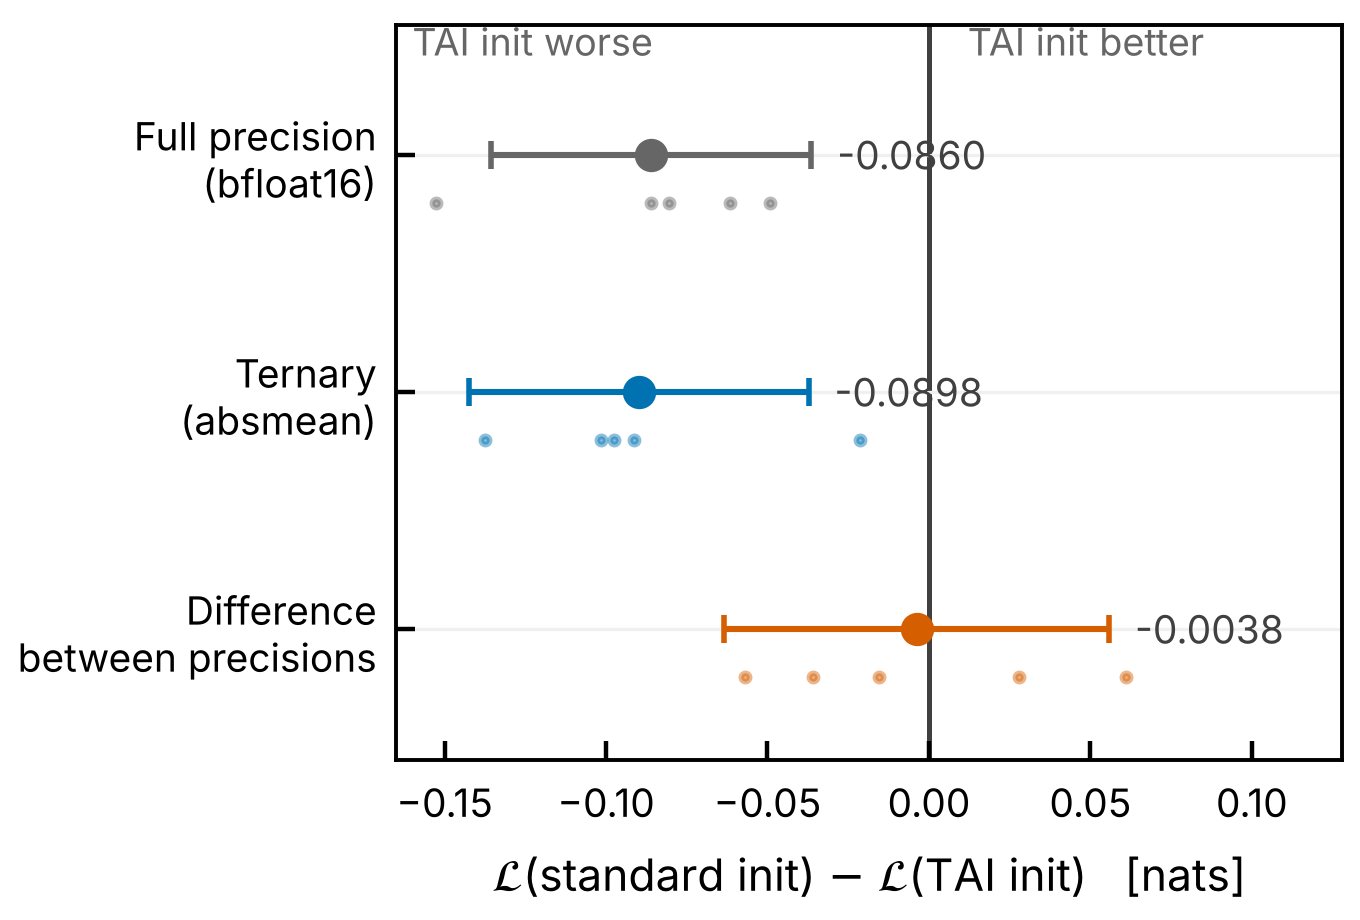
\includegraphics[width=0.8\linewidth]{fig8_init_ablation.png}
\caption{The $\{$full precision, ternary$\} \times \{$standard init, TAI
init$\}$ ablation at the primary scale ($n = 5$ seeds). Each row is the paired
initialization effect
$\mathcal{L}^{\mathrm{std\text{-}init}} - \mathcal{L}^{\mathrm{TAI\text{-}init}}$,
shown as the five per-seed values, their mean and its $95\%$ confidence
interval; negative values mean the TAI initializer attains the higher loss.
The penalty is of the same size under both precisions, and the difference
between them is indistinguishable from zero ($p = 0.869$), which is the
signature of a generically weaker initializer rather than of failed
operating-point control.}
\label{fig:initablation}
\end{figure}

The $\{$full precision, ternary$\} \times \{$standard init, TAI init$\}$ design
at the primary scale ($n = 5$ seeds) is assembled from three arms already in
the grid (\texttt{fp16\_control}, \texttt{standard} and \texttt{tai}) plus
one arm run specifically for it, \texttt{fp16\_taiinit}, which applies the TAI
initializer with quantization disabled. The design yields the initialization
effect
$\mathcal{L}^{\mathrm{std}} - \mathcal{L}^{\mathrm{TAI}}$ reported in
Table~\ref{tab:init2x2} and shown in Fig.~\ref{fig:initablation}.

\begin{table*}[t]
\centering
\small
\caption{Initialization $\times$ precision ablation at the primary scale
($n = 5$ seeds). The tabulated quantity is
$\mathcal{L}^{\mathrm{std\text{-}init}} - \mathcal{L}^{\mathrm{TAI\text{-}init}}$;
a negative value indicates that the standard initializer attains the lower
loss.}
\label{tab:init2x2}
\begin{tabular}{@{}lrr@{}}
\toprule
Precision & Initialization effect (nats) & Paired $t$-test $p$ \\
\midrule
Full precision (\texttt{bfloat16}) & $-0.0860$ & 0.0086 \\
Ternary (absmean) & $-0.0898$ & 0.0090 \\
\midrule
Difference between precisions & $-0.0038$ & 0.869 \\
\bottomrule
\end{tabular}
\end{table*}

The TAI initialization distribution carries a penalty of $0.086$ nats in full
precision and $0.090$ nats under ternary quantization. The two effects are of
the same sign, of nearly equal magnitude, and both significant at
$\alpha = 0.05$; the difference between them, $0.0038$ nats, is an order of
magnitude smaller than either, and the paired interaction contrast does not
resolve a difference ($t = +0.18$, $p = 0.869$, bootstrap 95\% CI
$[-0.035, +0.040]$); at $n = 5$ that interval is too wide to exclude an
interaction of half the size of either main effect, so what is established is
the absence of a detectable difference rather than equality. The
pre-registered discriminating pattern for
attributing the effect to operating-point control, a null effect in full
precision alongside a positive effect under quantization, is not observed:
neither leg holds, since the full-precision effect is significant and the
quantized effect runs opposite to the predicted direction.

%-----------------------------------------------------------------------------
\subsection{H6: behaviour across the scale ladder}
\label{sec:res-h6}

\begin{figure}[t]
\centering
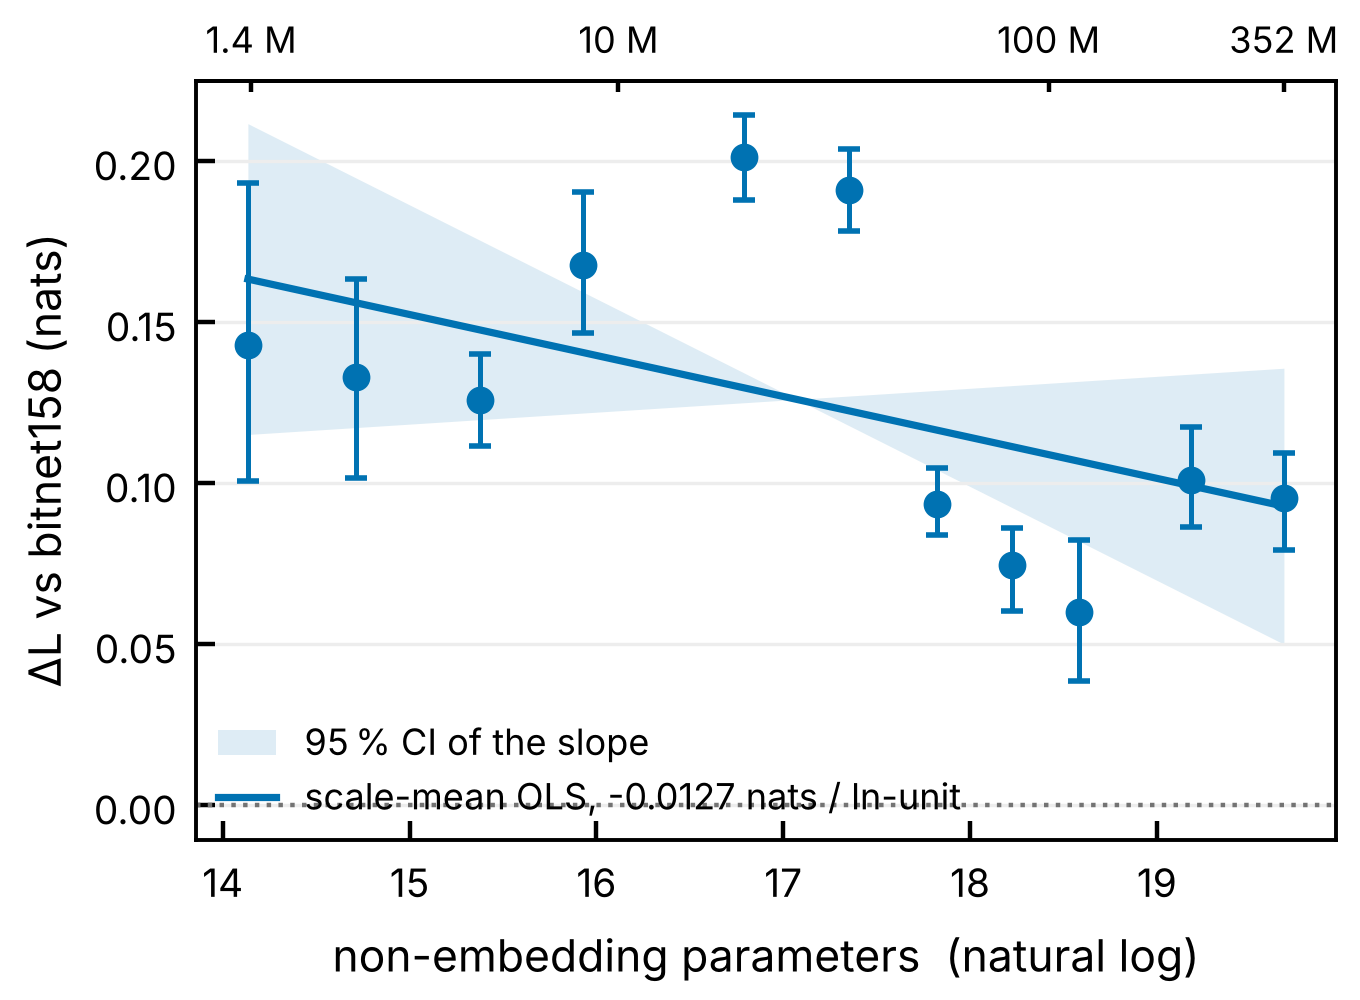
\includegraphics[width=0.86\linewidth]{fig6_scale.png}
\caption{The paired contrast of \texttt{tai\_warmup} against the
pre-registered baseline at each ladder point, with bootstrap 95\% confidence
intervals over seeds, and the primary scale-mean OLS slope of
Section~\ref{sec:res-h6} with its confidence interval. The slope is in nats
per natural log-unit of non-embedding parameters, and its interval spans zero.
The depth-controlled ladder is shown in Fig.~\ref{fig:twoslope}.}
\label{fig:scale}
\end{figure}

The primary readout is per-scale sign consistency. The effect
$\dL$ for \texttt{tai\_warmup} is positive at $11$ of $11$ ladder points
spanning $1.4$\,M to $352.3$\,M non-embedding parameters (binomial
$p = 0.0010$; Fig.~\ref{fig:scale}), with per-scale means listed in Table~\ref{tab:crossscale}. The
mean effect over scales is $+0.1260$ nats. Against the data-selected minimum
baseline, the exploratory sensitivity of Section~\ref{sec:res-h2}, the mean
effect is $+0.0818$ nats and the sign reverses at one scale.

The secondary slope diagnostic is reported with its estimator-dependence made
explicit, because the pre-registered mixed-effects model with a random
intercept per seed failed with a singular random-effects covariance, the
between-seed standard deviation of the effect being small relative to the
between-scale standard deviation. Table~\ref{tab:h6slope} reports the three
fallback estimators.

\begin{table*}[t]
\centering
\footnotesize
\caption{Slope of the \texttt{tai\_warmup} effect against $\log N$
(non-embedding parameters). The pre-registered mixed-effects estimator did not
converge. Clustering by seed treats scale-level variation as replicated within
seed and is anticonservative for a scale-level question; it is reported for
completeness only.}
\label{tab:h6slope}
\begin{tabular}{@{}llrrr@{}}
\toprule
Estimator & Unit & Slope & 95\% CI & $p$ \\
\midrule
Scale-mean OLS & scale ($n=11$) & $-0.0127$ & $[-0.0291,+0.0037]$ & 0.114 \\
Cluster-robust by scale & scale ($n=11$) & $-0.0126$ & $[-0.0236,-0.0016]$ & 0.024 \\
Cluster-robust by seed & seed ($n=15$) & $-0.0126$ & $[-0.0181,-0.0071]$ & $7.9\times 10^{-6}$ \\
Mixed-effects (pre-registered) & \multicolumn{4}{l}{failed: singular random-effects covariance} \\
\midrule
Depth-controlled ladder & scale ($n=4$) & $-0.0553$ & $[-0.0701,-0.0392]$ & n/a \\
\bottomrule
\end{tabular}
\end{table*}

All estimators agree on the point estimate ($\approx -0.0126$ nats per natural
log-unit of parameters) and on the sign: the effect narrows as scale grows. The
scale-level interval, which is the appropriate unit for a scale-level question,
spans zero under OLS and excludes zero marginally under cluster-robust
inference. The operative statement is accordingly that the direction is
consistent across scale while the magnitude is not resolved as
scale-varying. The corresponding slopes for the auxiliary outcomes, fitted with the same
scale-mean estimator against the same baseline, are $-16.47$ steps per
log-unit for steps-to-target (95\% CI $[-27.49, -5.44]$) and $-0.0056$ for the
sparsity gap (95\% CI $[-0.0093, -0.0019]$). Extrapolations from these fits are labelled as
predictions and are not treated as evidence.

One confound has to be ruled out before the slope can be read as a statement
about scale at all, since width and depth co-vary along the principal ladder.
The depth-controlled ladder
(Table~\ref{tab:widthonly}, Fig.~\ref{fig:twoslope}), in which depth is fixed at
$L=6$ and only width varies, reproduces the sign of the main-ladder slope with a
steeper magnitude ($-0.0553$, 95\% CI $[-0.0701, -0.0392]$). The narrowing
trend is therefore not an artefact of depth co-varying with width along the
principal ladder.

\begin{table*}[t]
\centering
\small
\caption{Depth-controlled (width-only) ladder, $L = 6$ fixed, $n = 5$ seeds.
Held-out loss in nats per token, mean $\pm$ SD; $\dL$ is the paired contrast of
\texttt{tai\_warmup} against \texttt{bitnet158}, following Eq.~\eqref{eq:dL}.}
\label{tab:widthonly}
\begin{tabular}{@{}lrrrr@{}}
\toprule
Scale & \texttt{standard} & \texttt{bitnet158} & \texttt{tai\_warmup} & $\dL$ \\
\midrule
\texttt{wc384} & $5.1397 \pm 0.0298$ & $5.1402 \pm 0.0304$ & $4.9710 \pm 0.0196$ & $+0.169$ \\
\texttt{wc512} & $4.9683 \pm 0.0205$ & $4.9684 \pm 0.0173$ & $4.8487 \pm 0.0283$ & $+0.120$ \\
\texttt{wc768} & $4.8489 \pm 0.0141$ & $4.9196 \pm 0.0142$ & $4.7603 \pm 0.0138$ & $+0.159$ \\
\texttt{wc1024} & $4.9382 \pm 0.0198$ & $4.9375 \pm 0.0265$ & $4.8831 \pm 0.0107$ & $+0.054$ \\
\bottomrule
\end{tabular}
\end{table*}

\begin{figure}[t]
\centering
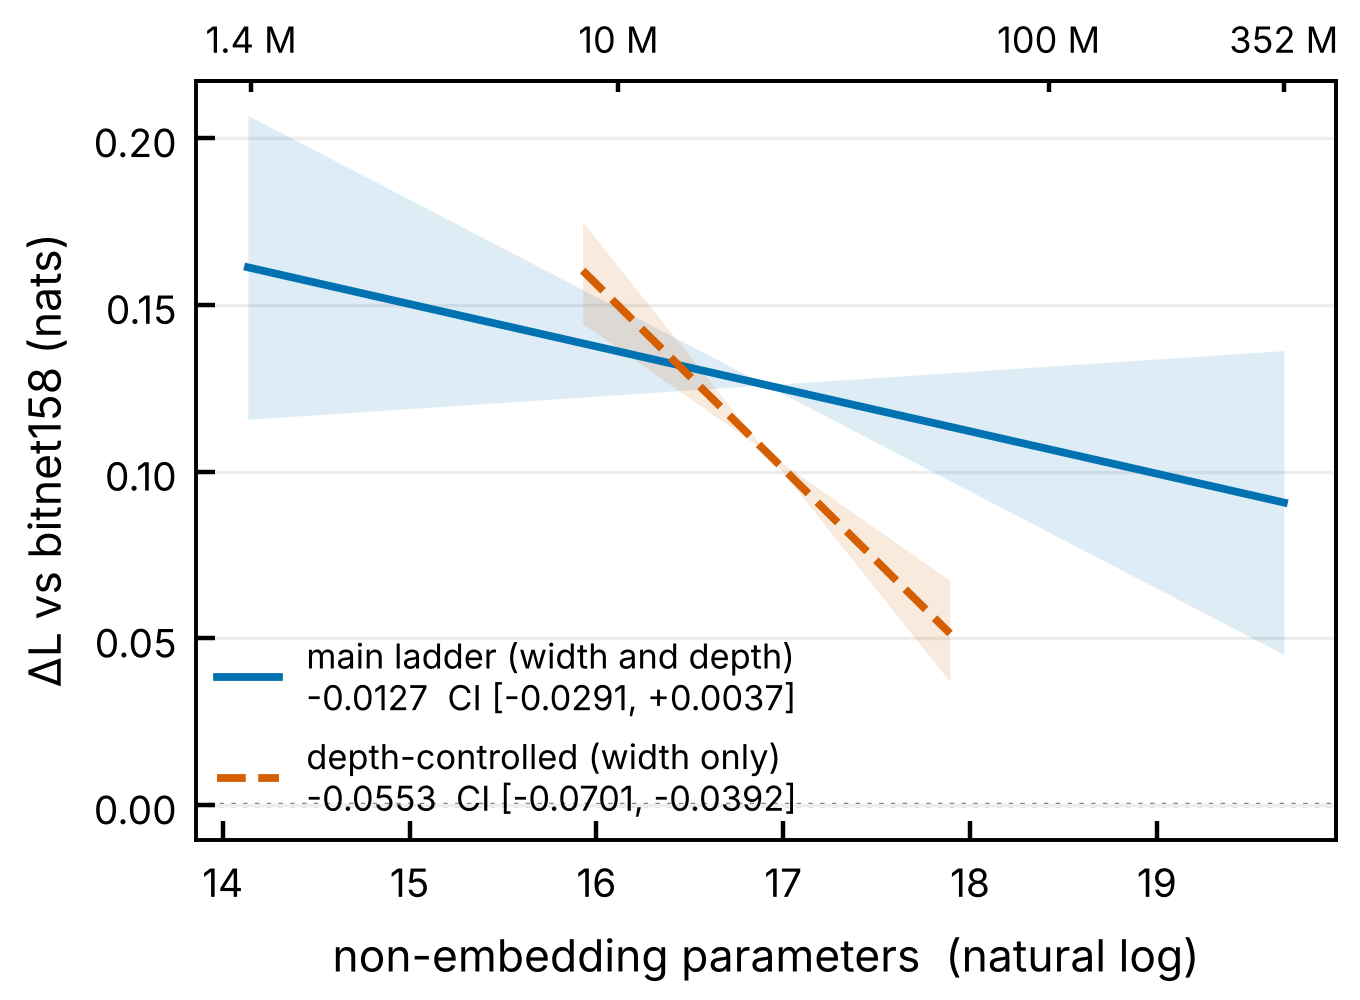
\includegraphics[width=0.86\linewidth]{fig9_two_slope.png}
\caption{Scaling slope estimated with width and depth varying together,
against the depth-controlled ladder in which depth is held fixed at $L = 6$.
Both slopes are in nats per natural log-unit of non-embedding parameters, and
each band is the $95\%$ confidence interval of its slope. The depth-controlled
fit is the steeper of the two and its interval excludes zero; the main-ladder
interval does not.}
\label{fig:twoslope}
\end{figure}

%-----------------------------------------------------------------------------
\subsection{The mechanism-matched control at its default operating point}
\label{sec:res-gammadefault}

Sections~\ref{sec:res-h3} and~\ref{sec:res-mechanism} compare
\texttt{gamma\_offset} against \texttt{tai} at matched $\rhoz$. Because
the arm also appears in the main grid at the single default $\rhoz = 0.75$, its
contrast against the pre-registered baseline is reported separately here; the
two questions have different answers and conflating them would overstate the
control.

Against \texttt{bitnet158} at the default operating point,
\texttt{gamma\_offset} attains the lower held-out loss at $7$ of the $11$
ladder points (binomial $p = 0.55$). The sign is scale-dependent and changes
once: the arm is worse at the four smallest scales (significantly so at
\texttt{dim384}, $\dL = -0.0251$, $p = 7.0\times 10^{-3}$) and better at the
seven largest, significantly at five of them, reaching $\dL = +0.0643$
($p = 1.4\times 10^{-4}$) at \texttt{dim1024} and $+0.0480$
($p = 3.1\times 10^{-4}$) at \texttt{dim1536}. A single fixed threshold
constant is therefore not uniformly preferable to the absmean convention at
this budget; the sweep of Table~\ref{tab:sweep} shows that its advantage
requires $\rhoz$ to be tuned, and that the tuned optimum itself moves with
scale ($0.70$ at \texttt{dim384}, $0.80$ at \texttt{dim768}).

\subsection{H7: transfer to a second architecture family}
\label{sec:res-h7}

Three arms were re-run on block family B (grouped-query attention with SwiGLU
feed-forward) at two scales, $15$ seeds each. For \texttt{tai\_warmup} the sign
of the effect is preserved at both: $\dL = +0.0794$
($p = 1.9\times 10^{-4}$, $n = 15$) at \texttt{dim256} and $\dL = +0.0347$
($p = 8.3\times 10^{-4}$, $n = 15$) at \texttt{dim384}.

For \texttt{gamma\_offset} at its default $\rhoz = 0.75$ the sign is
not preserved: the arm is significantly worse than the baseline on
family B at both scales, $\dL = -0.0424$ ($p = 3.7\times 10^{-3}$) at
\texttt{dim256} and $\dL = -0.0873$ ($p = 2.2\times 10^{-8}$) at
\texttt{dim384}, the latter being the largest deficit recorded for that arm
anywhere in the study. Table~\ref{tab:archB} reports both contrasts. No
$\rhoz$ sweep was executed on family B, so it is not known whether a
re-tuned threshold constant would recover the deficit; the retention property
of the threshold mechanism was likewise measured only on family A. Aggregated
over the $13$ independent (architecture $\times$ scale) cells for which a sign
is available, the effect favours \texttt{tai\_warmup} in all $13$ against the
pre-registered baseline (binomial $p = 2.4\times 10^{-4}$); against the
data-selected minimum baseline it is $12$ of $13$, the discordant cell being
\texttt{dim1024} on family A.
Magnitudes for \texttt{tai\_warmup} on family B are smaller than the
corresponding family-A values ($+0.133$ and $+0.168$ at the same two
scales).

\begin{table*}[t]
\centering
\small
\caption{Cross-architecture contrasts on block family B (GQA $+$ SwiGLU),
paired against \texttt{bitnet158} over $15$ seeds. $\dL$ follows
Eq.~\eqref{eq:dL}; positive favours the arm. Family-A values at the same scales
are reproduced from Table~\ref{tab:crossscale} and
Section~\ref{sec:res-gammadefault} for comparison.}
\label{tab:archB}
\begin{tabular}{@{}llrrr@{}}
\toprule
Scale & Arm & $\dL$ (family B) & $p_t$ & $\dL$ (family A) \\
\midrule
\texttt{dim256} & \texttt{tai\_warmup} & $+0.0794$ & $1.9\times 10^{-4}$ & $+0.1329$ \\
& \texttt{gamma\_offset} & $-0.0424$ & $3.7\times 10^{-3}$ & $-0.0032$ \\
\texttt{dim384} & \texttt{tai\_warmup} & $+0.0347$ & $8.3\times 10^{-4}$ & $+0.1677$ \\
& \texttt{gamma\_offset} & $-0.0873$ & $2.2\times 10^{-8}$ & $-0.0251$ \\
\bottomrule
\end{tabular}
\end{table*}

%-----------------------------------------------------------------------------
\subsection{H8: feedback of the sweep-optimal operating point}
\label{sec:res-h8}

Re-running the grid with $\rhoz^\star = 0.70$ as the \texttt{tai\_star} arm
($30$ runs at \texttt{dim384} and \texttt{dim768}) does not recover the deficit
of the fixed-$\rhoz$ initialization variant. At \texttt{dim384},
\texttt{tai\_star} attains $5.1919$ nats against $5.1914$ for \texttt{tai} at
$\rhoz = 0.75$, i.e.\ $\dL = -0.0805$ against the baseline; at
\texttt{dim768} it attains $5.0382$ against $5.0370$, $\dL = -0.1214$.

The comparison is not a pure change of $\rhoz$. Per-arm calibration
(Section~\ref{sec:lrcal}) gives \texttt{tai\_star} an $\eta^{\star}$ of
$2\times 10^{-3}$ at \texttt{dim384} against $3\times 10^{-3}$ for
\texttt{tai}, which is why its final sparsity ($28.4\%$) falls below the
$30.2\%$ the sweep records at the same $\rhoz = 0.70$, rather than above
\texttt{tai}'s $30.0\%$ as the monotone relation of
Section~\ref{sec:res-h3} would predict. At \texttt{dim768} the two arms
calibrate to the same rate and their sparsities agree ($29.8\%$ versus
$29.5\%$). This is also the one contrast in the study drawn across the
execution-path split of Section~\ref{sec:res-validity}, \texttt{tai\_star}
falling in the fast group at \texttt{dim384} and the baseline in the slow one;
at \texttt{dim768} both arms lie in the same group and the deficit is
unchanged, which is the comparison the conclusion rests on.

Both contrasts are significant, and for both the null is rejected under
Holm--Bonferroni within the confirmatory family. The steps-to-target deficit is reduced at \texttt{dim384}
($\dS = -35$ for \texttt{tai\_star} versus $-59$ for \texttt{tai}) and
unchanged at \texttt{dim768} ($-95$ in both). H8 is therefore not supported:
feeding back the sweep-optimal operating point neither degrades nor materially
improves the fixed-$\rhoz$ arm.

%-----------------------------------------------------------------------------
\subsection{Downstream evaluation}
\label{sec:res-downstream}

\begin{figure}[t]
\centering
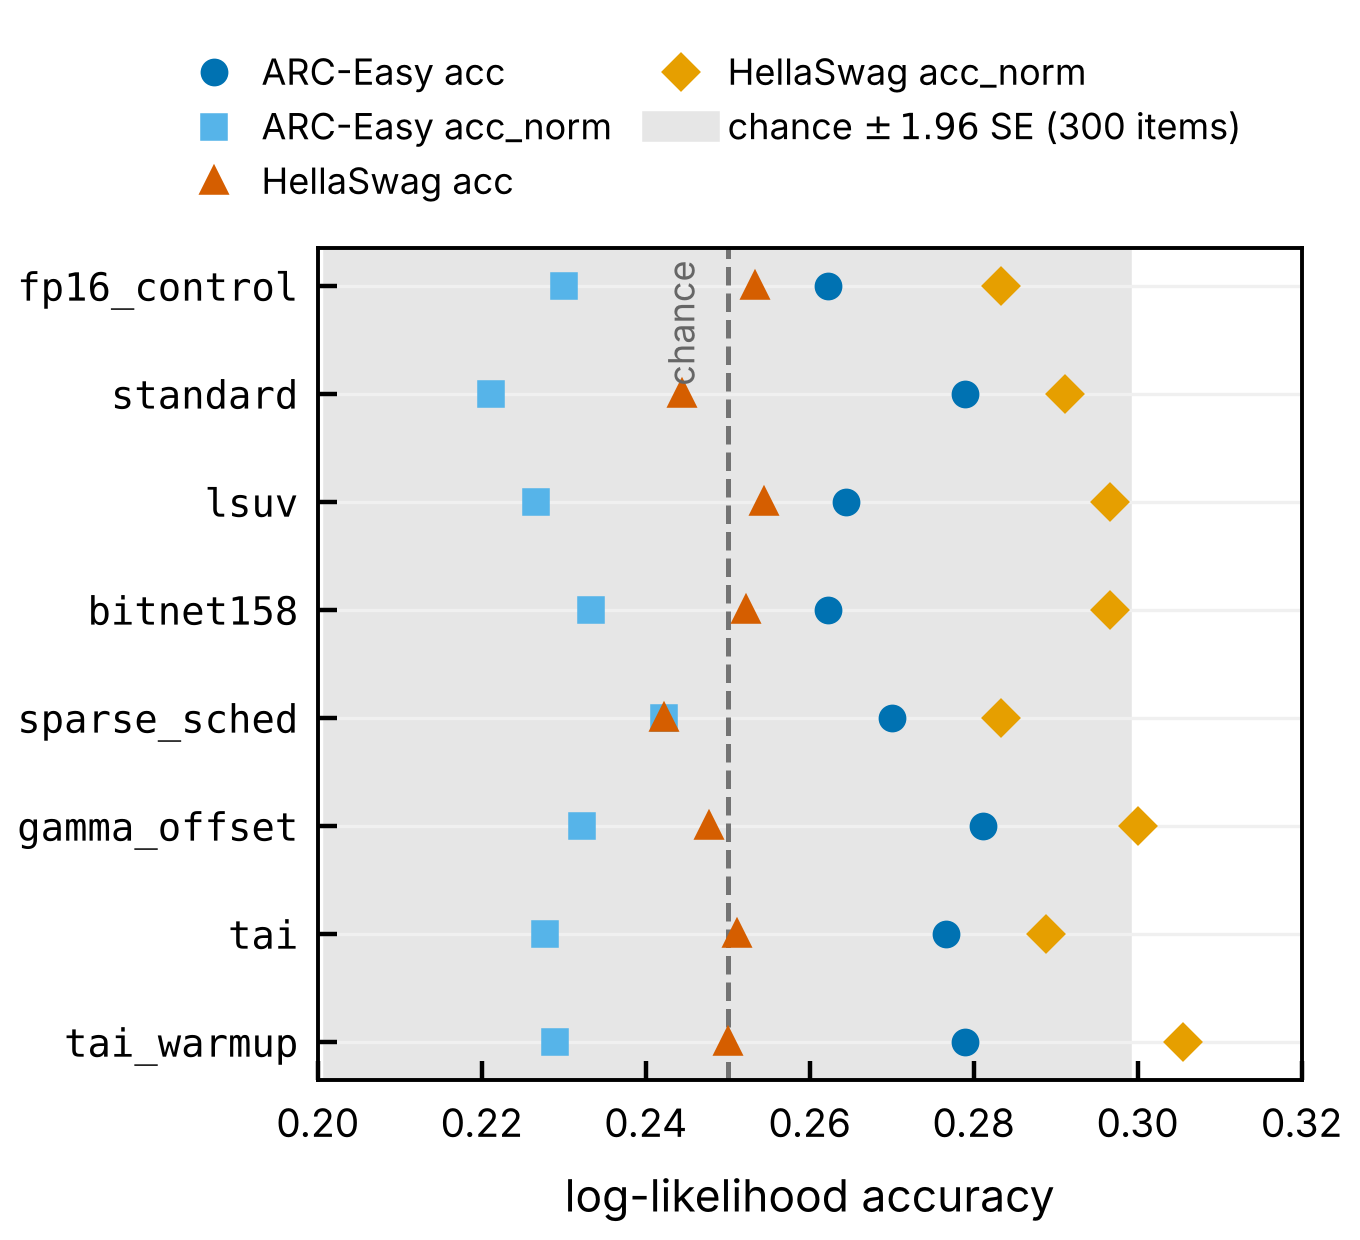
\includegraphics[width=0.9\linewidth]{fig4_lmeval.png}
\caption{Zero-shot accuracy on ARC-Easy and HellaSwag under log-likelihood
scoring, by arm, at the primary scale on the same $300$ scored items as
Table~\ref{tab:lmeval}. Both token-normalized (acc) and byte-normalized
(acc\_norm) metrics are shown. The shaded band is the random-choice rate plus
or minus $1.96$ sampling standard errors for a $300$-item subset; every
observation falls inside it.}
\label{fig:lmeval}
\end{figure}

Table~\ref{tab:lmeval} reports the four benchmark metrics at the primary
scale, and Fig.~\ref{fig:lmeval} shows them across the arm set.

\begin{table*}[t]
\centering
\small
\caption{Downstream log-likelihood accuracy at the primary scale, scored on the
first three seeds of each cell so that the comparison remains paired
($300$ items per task). $\Delta$ is the paired difference against
\texttt{bitnet158}; $p_t$ is the paired $t$-test $p$-value. Random-choice
baselines are approximately $0.25$ for both tasks.}
\label{tab:lmeval}
\begin{tabular}{@{}llrrrr@{}}
\toprule
Task / metric & Arm & Arm acc. & Baseline acc. & $\Delta$ & $p_t$ \\
\midrule
ARC-Easy (acc) & \texttt{tai} & 0.277 & 0.262 & $+0.014$ & 0.423 \\
& \texttt{tai\_warmup} & 0.279 & 0.262 & $+0.017$ & 0.138 \\
ARC-Easy (acc\_norm) & \texttt{tai} & 0.228 & 0.233 & $-0.006$ & 0.797 \\
& \texttt{tai\_warmup} & 0.229 & 0.233 & $-0.004$ & 0.673 \\
HellaSwag (acc) & \texttt{tai} & 0.251 & 0.252 & $-0.001$ & 0.921 \\
& \texttt{tai\_warmup} & 0.250 & 0.252 & $-0.002$ & 0.754 \\
HellaSwag (acc\_norm) & \texttt{tai} & 0.289 & 0.297 & $-0.008$ & 0.465 \\
& \texttt{tai\_warmup} & 0.306 & 0.297 & $+0.009$ & 0.490 \\
\bottomrule
\end{tabular}
\end{table*}

No benchmark contrast is significant at any scale after correction, and the
observed differences ($|\Delta| \leq 0.025$) are of the order of the sampling
noise of a $300$-item subset, $\sqrt{p(1-p)/300} \approx 0.025$ at the
random-choice rate. Absolute
accuracies lie between $0.21$ and $0.31$ across all arms, tasks and metrics,
i.e.\ at or marginally above the random-choice baseline. Aggregated over the
$88$ benchmark contrasts computed across the ladder, three reach nominal
$p < 0.05$, which is consistent with the number expected by chance.

The internal transfer proxy is the sole downstream measure that discriminates
between arms. Next-token top-1 accuracy at the primary scale is $0.242$ for
\texttt{tai\_warmup} against $0.227$ for the baseline
($p < 10^{-4}$) and $0.221$ for \texttt{tai} ($p < 10^{-4}$); the ordering of
these three arms matches their held-out loss ordering at every scale.

%-----------------------------------------------------------------------------
\subsection{Ablations}
\label{sec:res-ablations}

\subsubsection{Realization map of the TAI construction}

The separation condition of Lemma~\ref{lem:separation} was probed over a
$5 \times 3$ grid in the dormant magnitude $\delta$ and jitter half-width $a$
at target $\rhoz = 0.75$. In $11$ of $15$ cells the condition holds and the
target is realized to $|\rho_{\mathrm{real}} - \rhoz| \leq 1.3\times 10^{-4}$,
independently of $(\delta, a)$; in the remaining four cells
($\delta = 0.45$ at every $a$, and $\delta = 0.35$ with $a = 0.30$) the
assertion fires and the target is not realizable. The boundary is thus located
empirically and matches the analytical prediction, and the operating defaults
$(\delta, a) = (0.15, 0.15)$ sit in the interior of the valid region.

\subsubsection{Quality sensitivity to the dormant magnitude}

Although $\rho_{\mathrm{real}}$ is invariant to $\delta$ within the valid
region, final quality is not. At fixed $\rhoz = 0.75$ and $n = 5$ seeds, mean
held-out loss falls monotonically from $5.2304 \pm 0.0466$ at $\delta = 0.05$
to $5.1048 \pm 0.0202$ at $\delta = 0.35$, a spread of $0.126$ nats
(one-way ANOVA $F = 12.11$, $p = 2.2\times 10^{-4}$; exploratory, outside the
Holm family). The construction therefore exposes a second effective degree of
freedom whose influence on quality is comparable in magnitude to the
$\rhoz$ effect itself.

\subsubsection{$\gamma$-warmup schedule grid}

The $3 \times 3$ grid over warmup start $s_0$ and duration $\tau_w$ at the
primary scale ($n = 5$ seeds) is reported in Table~\ref{tab:warmupgrid}.
The best cell is $(s_0, \tau_w) = (0.4, 120)$ at $5.0437$ nats and the worst
is $(0.5, 480)$ at $5.1838$; loss increases monotonically in $\tau_w$ at every
$s_0$, and $s_0 = 0.5$ is dominated by $s_0 = 0.4$ at every $\tau_w$. The
grid-default configuration used in the main grid, $(0.4, 240)$, is the second-best cell ($5.0514$).

\begin{table}[t]
\centering
\small
\caption{$\gamma$-warmup ablation at the primary scale (\texttt{dim384}): mean
held-out loss in nats per token over $5$ seeds, as a function of the warmup
start $s_0$ and the duration $\tau_w$ in optimizer steps.}
\label{tab:warmupgrid}
\begin{tabular}{@{}lrrr@{}}
\toprule
$s_0 \backslash \tau_w$ & 120 & 240 & 480 \\
\midrule
0.3 & 5.0536 & 5.1249 & 5.1564 \\
0.4 & \textbf{5.0437} & 5.0514 & 5.1130 \\
0.5 & 5.1553 & 5.1568 & 5.1838 \\
\bottomrule
\end{tabular}
\end{table}

\subsubsection{Learning-rate sensitivity}

Across the five-point learning-rate grid at the primary scale
(Table~\ref{tab:lrsens}), \texttt{tai\_warmup} attains the lower loss at four
of five settings; the ordering reverses only at the smallest rate
($5\times 10^{-4}$), where both arms are far from their optima. At the baseline's own
optimum ($3\times 10^{-3}$), where the comparison is least favourable to
\texttt{tai\_warmup}, the advantage is $0.218$ nats, and it is larger still at
$5\times 10^{-3}$ ($0.250$). The reported conclusion is therefore not an artefact of a single
optimizer setting.

\begin{table}[t]
\centering
\small
\caption{Learning-rate sensitivity at the primary scale (\texttt{dim384},
$n = 5$ ablation seeds). Entries are mean held-out loss $\mathcal{L}$ in
nats/token; $\dL$ is the paired contrast against \texttt{standard}, the
comparison arm of this ablation, so positive favours
\texttt{tai\_warmup}. The baseline's minimum over the grid ($5.1196$ at
$3\times 10^{-3}$) is interior and therefore a genuine envelope;
\texttt{tai\_warmup} falls below it at the three largest rates, which excludes
the global effective-learning-rate account of the schedule
(Section~\ref{sec:disc-timing}).}
\label{tab:lrsens}
\begin{tabular}{@{}lrrr@{}}
\toprule
Peak LR & \texttt{standard} & \texttt{tai\_warmup} & $\dL$ \\
\midrule
$5\times 10^{-4}$ & 5.7185 & 5.8034 & $-0.085$ \\
$1\times 10^{-3}$ & 5.4115 & 5.3928 & $+0.019$ \\
$2\times 10^{-3}$ & 5.1893 & 5.0409 & $+0.148$ \\
$3\times 10^{-3}$ & 5.1196 & 4.9019 & $+0.218$ \\
$5\times 10^{-3}$ & 5.1891 & 4.9390 & $+0.250$ \\
\bottomrule
\end{tabular}
\end{table}

%-----------------------------------------------------------------------------
\subsection{Efficiency}
\label{sec:res-eff}

Table~\ref{tab:efficiency} separates the theoretical deployment model from the
measured simulation cost, in the order specified by the protocol.

\begin{table*}[t]
\centering
\scriptsize
\caption{Efficiency. Panel (A) is a counting argument over the ternary codebook
at the largest \emph{declared} configuration, \texttt{dim2048}, which was not
executed (Section~\ref{sec:res-validity}); the compression ratios do not depend
on the parameter count, so only the absolute sizes are specific to it. It is
independent of the hardware used here.
Panel (B) is the measured cost of simulating ternary arithmetic in
\texttt{bfloat16} under straight-through estimation; it is a property of the
research harness and is not a ternary-inference measurement. No ternary kernel
was benchmarked in this work.}
\label{tab:efficiency}
\begin{tabular}{@{}lrr@{}}
\toprule
\multicolumn{3}{@{}l}{\textbf{(A) Deployment model (theoretical, primary)}} \\
\midrule
Quantized parameters & \multicolumn{2}{r}{782.91\,M} \\
Half-precision size & \multicolumn{2}{r}{1493.28\,MB} \\
Ternary size, information-theoretic ($\log_2 3 = 1.585$ bits/weight) & \multicolumn{2}{r}{147.92\,MB} \\
Ternary size, 2-bit packed & \multicolumn{2}{r}{186.66\,MB} \\
Compression vs.\ half precision (information-theoretic) & \multicolumn{2}{r}{$10.09\times$} \\
Compression vs.\ half precision (2-bit packed) & \multicolumn{2}{r}{$8.00\times$} \\
\midrule
\multicolumn{3}{@{}l}{\textbf{(B) Simulation cost (measured, secondary)}} \\
\midrule
& \texttt{fp16\_control} & ternary (simulated) \\
Latency & 430.9\,ms & 718.9\,ms \\
Throughput & 38{,}025 tok/s & 22{,}792 tok/s \\
Peak memory & 3.336\,GB & 3.336\,GB \\
Forward sparsity & 0.0\% & 25.0\% \\
Latency ratio & \multicolumn{2}{r}{$1.67\times$} \\
\bottomrule
\end{tabular}
\end{table*}

The simulated ternary path is $1.67\times$ slower than the full-precision
control at identical peak memory, which is the expected direction: under
straight-through estimation the ternary path executes the same
\texttt{bfloat16} matrix multiplication and additionally performs
normalization, activation quantization, weight quantization and rescaling,
while retaining \texttt{bfloat16} master weights. This quantity is charged
honestly to the method in the compute-equal accounting and carries no
deployment implication in either direction.

%-----------------------------------------------------------------------------
\subsection{Summary of pre-registered outcomes}
\label{sec:res-summary}

Table~\ref{tab:hypsummary} consolidates the outcome of each pre-registered
hypothesis under the wording licensed by Section~\ref{sec:res-budget}.

\begin{table*}[t]
\centering
\scriptsize
\caption{Outcome of every pre-registered hypothesis. Token-equal indicates
that the claim is restricted to performance at the fixed $20$\,M-token budget,
convergence not having been established for any arm.}
\label{tab:hypsummary}
\begin{tabular}{@{}p{0.9cm}p{2.7cm}p{6.1cm}@{}}
\toprule
Hyp. & Outcome & Operative statement \\
\midrule
H1 & Split &
Supported for \texttt{tai\_warmup} ($11/11$ scales, $\dS$ up to $+148$ steps);
rejected in the opposite direction for \texttt{tai} ($11/11$ scales slower). \\
\addlinespace
H2 & Untestable (pre-reg.) &
No run reached plateau ($0/760$); the convergence-conditional equivalence test
has an empty qualifying set. The token-equal companion returns
\texttt{tai\_warmup} superior at $11/11$ scales and \texttt{tai} inferior at
$10/11$; equivalence is never returned. \\
\addlinespace
H3 & Not supported (strong form) &
Ordinal control is near-perfect (per-seed Spearman $-0.996$, SNR $44.9\times$)
and the placebo is flat, but retention for the initialization mechanism is
$0.052$--$0.069$: $93$--$95\%$ of the intervention is erased, and final
sparsity converges to an attractor near $0.30$. The threshold-offset mechanism
retains $1.003$--$1.006$. \\
\addlinespace
H4 & Supported &
No evidence of variance inflation on the pooled seed $\times$ fold matrix
($W = 0.554$, $p = 0.458$); $23/24$ per-cell Levene tests are non-significant
and the one exception favours lower TAI variance. \\
\addlinespace
H5 & Supported for the threshold mechanism &
The threshold-offset arm traces a U-shaped frontier spanning $50$ points of
sparsity with an interior optimum; the initialization arm's sparsity axis spans
$2.6$ points, rendering its frontier near-degenerate.
$\rhoz^\star = 0.70$ (bootstrap $P = 0.758$). \\
\addlinespace
H6 & Direction supported; magnitude unresolved &
Sign positive at $11/11$ scales (binomial $p = 0.0010$) over $1.4$\,M--$352$\,M
parameters. Slope $-0.0127$ per log-unit under the scale-level OLS estimator,
whose interval spans zero. The depth-controlled ladder reproduces the sign. \\
\addlinespace
H7 & Supported for \texttt{tai\_warmup}; not for \texttt{gamma\_offset} &
Sign preserved for \texttt{tai\_warmup} on family B at both tested scales
($p \leq 8.3\times 10^{-4}$); all $13$ architecture $\times$ scale cells
consistent against the pre-registered baseline (binomial
$p = 2.4\times 10^{-4}$), $12/13$ against the data-selected minimum. \texttt{gamma\_offset} at its default
$\rhoz$ is significantly worse than the baseline on family B at both scales
(Table~\ref{tab:archB}). \\
\addlinespace
H8 & Not supported &
\texttt{tai\_star} at $\rhoz^\star = 0.70$ tracks \texttt{tai} to within
$0.0013$ nats at both tested scales and remains below the baseline. \\
\bottomrule
\end{tabular}
\end{table*}

Two auxiliary controls complete the picture. The mechanism-matched contrast
places the quality difference in \texttt{gamma\_offset}'s favour at
$0.0610$ nats, 95\% CI $[+0.0474, +0.0742]$, over $90$ paired cells at matched
$\rhoz$, though, as Sections~\ref{sec:res-gammadefault} and~\ref{sec:res-h7}
record, that arm's advantage over the baseline is scale-dependent on
family A and reverses on family B. The $2 \times 2$ ablation finds the TAI
initialization distribution to carry an almost identical penalty in full
precision ($-0.086$ nats) and under quantization ($-0.090$ nats), so the
pre-registered pattern that would attribute the effect to ternary
operating-point control is not observed.

Taken together, the results separate cleanly into three groups: what the
initialization intervention does (little, and durably almost nothing), what the
threshold intervention does (everything the initialization was supposed to do,
with caveats of its own), and what annealing the threshold does (the largest
and most consistent effect in the study). Section~\ref{sec:discussion} takes
each group in turn and asks why the quantizer's own definition makes this
separation almost inevitable.

%=============================================================================

%=============================================================================

\section{Discussion}
\label{sec:discussion}

%-----------------------------------------------------------------------------
\subsection{What the experiment establishes, and what it does not}
\label{sec:disc-summary}

It is worth stating plainly, and early, that this study did not confirm the
hypothesis it was designed to confirm. The pre-registered claim was that
shaping the initial weight-magnitude distribution so as to place a ternary
network at a chosen operating point $\rhoz$ would improve both convergence
speed and final quality, and would causally determine the sparsity the network
eventually learns. Of these, the first is supported only for the schedule
variant, the second is reversed for the fixed-$\rhoz$ variant, and the third is
supported for a mechanism that is not the proposed one. The value of the work
lies in the sharpness with which the design separates these outcomes, and we
have organised the discussion around that separation rather than around a
defence of the original claim.

Three findings survive scrutiny, and they are of unequal importance.

First, and least contentious: the ternary operating point is analytically
locked and the lock is real. For any zero-mean initializer, the absmean rule
places the network at $\rhoz = 0.6899$ irrespective of the initialization
scale, and the measurement confirms this across two orders of magnitude in
$\sigma$, over which the empirical active fraction varies by $6\times10^{-4}$,
and across four initializer families, all of which land within $10^{-3}$ of
the analytical value (Table~\ref{tab:locked}). This is a small analytical observation, but it has a
practical consequence that the quantization literature has not made explicit:
in an absmean ternary network, initialization scale is not a lever on sparsity,
and any study that varies $\sigma$ hoping to trade quality against density is
varying nothing.

Second, and most important: the two mechanisms that can move the
operating point behave completely differently under training. The threshold
offset \texttt{gamma\_offset} retains its target essentially perfectly ($r = 1.003$ and $1.006$ at the two
tested scales, $R^{2} = 1.000$); an initialization intervention of identical
nominal magnitude is almost entirely erased ($r = 0.052$ and $0.069$). A
$50$-percentage-point manipulation of initial sparsity leaves $50$ points of
final sparsity in the first case and between $2.6$ and $3.6$ points in the
second. We regard this contrast, rather than the performance of any single
arm, as the central empirical result of the paper, and Section~\ref{sec:disc-attractor} is devoted to why it arises.

Third: annealing the threshold works, and does so consistently. The
$\gamma$-warmup arm \texttt{tai\_warmup} attains a lower held-out loss
$\mathcal{L}$ and reaches its scale's pre-registered target loss
($\mathcal{L}_{\mathrm{target}} = 5.6539$ at the primary scale) in fewer steps
than the frozen primary baseline \texttt{bitnet158} at $11$ of $11$ scales
spanning $1.4$\,M--$352$\,M non-embedding parameters, at all $13$
architecture~$\times$~scale cells, and at four of five learning rates. The
effect is not fragile with respect to seed, fold, architecture family, depth,
or optimizer setting. Whether it is fragile with respect to training
budget is the principal open question, and we treat it at length in
Section~\ref{sec:disc-budget}.

Against these, three pre-registered claims failed, and the reasons are
instructive rather than merely negative: the fixed-$\rhoz$ initializer
\texttt{tai} is a worse initializer in full precision as well as under
quantization (Section~\ref{sec:disc-attribution}); the mechanism-matched
control \texttt{gamma\_offset} outperforms it at matched $\rhoz$
(Section~\ref{sec:disc-attribution}); and the feedback of the sweep-optimal
operating point, \texttt{tai\_star}, had almost no room to change anything, for
reasons that are a consequence of the retention result itself
(Section~\ref{sec:disc-designcritique}).

One qualification must be carried through everything that follows, because it
bounds the strongest reframing these data will support. That
\texttt{gamma\_offset} beats \texttt{tai} at matched $\rhoz$ is robust
($+0.0610$ nats, $95\%$ CI $[+0.0474,+0.0742]$, $90$ paired cells). That
\texttt{gamma\_offset} beats the baseline is not a general fact: at its
default $\rhoz = 0.75$ it does so at only seven of eleven scales on family~A,
with the sign turning over mid-ladder, and it is significantly worse
than the baseline on family~B at both tested scales
(Section~\ref{sec:res-h7}). The durability of the threshold mechanism and the
competitiveness of any particular threshold constant are separate claims, and
only the first is established here.

%-----------------------------------------------------------------------------
\subsection{Why the initialization intervention is erased: the absmean
attractor}
\label{sec:disc-attractor}

The retention asymmetry has a straightforward explanation, and articulating it
is the main theoretical contribution we can defend.

The absmean threshold is not an external constant. It is a functional of the
weight matrix itself,
\begin{equation}
\label{eq:selfref}
\gamma(\Wm; c) \;=\; c\,\E|w|,
\end{equation}
so the criterion by which a weight is judged large enough to survive moves
whenever the weight distribution moves. An initialization intervention perturbs
the numerator and the denominator of the same ratio: TAI shapes $|w|$ into two
modes, but $\E|w|$ is computed from those same modes, and the surviving
fraction is determined only by where the modes sit relative to their own
mean. Gradient descent then acts on the weights, and as it does so it drags
$\gamma$ along with them. The threshold is, in this precise sense, adaptive;
nothing in the training dynamics preserves the initial partition, and the
system relaxes to whatever active fraction the optimizer's own steady-state
magnitude distribution implies.

The measurements are consistent with exactly this picture. The fitted fixed
point of the retention regression is $0.305$ at \texttt{dim384} and $0.300$ at
\texttt{dim768}, and the untouched \texttt{standard} arm lands at $0.321$ and
$0.318$ respectively. All four straddle the analytical initialization value
$1 - \rhoz = 0.310$ within $0.011$, the fitted attractors falling just below
it and the untouched arm just above. In other words, the value
$\approx 0.31$ that Proposition~\ref{prop:locked} identifies as a property of
initialization turns out to be approximately where the optimizer goes
anyway. This reframes the premise of the paper in a way we did not anticipate:
the locked operating point is not merely a shared default that every zero-mean
initializer happens to inherit; it is close to an attractor of ternary training
under this quantizer.

A threshold offset escapes this because it changes the constant $c$, which no
gradient touches. The survival condition $|w| \geq \tfrac{c}{2}\E|w|$ is
homogeneous of degree zero in the weights, so rescaling the weights cannot undo
a change in $c$; only a change in the shape of the magnitude
distribution could, and the observed $R^{2} = 1.000$ indicates that shape
change is negligible over the tested range. The consequence is a clean
prediction that we did not test and that a follow-up study should:
any quantizer whose threshold is a fixed multiple of a
distribution statistic of the current weights will exhibit low retention of
initialization interventions, while any quantizer whose threshold is constant
in the weights will retain them. Trained ternary quantization
\cite{zhu2017a} falls on the first side of this line despite learning its
per-layer scaling factors, because its threshold is a fixed multiple of
$\max|w|$ and therefore moves with the weights exactly as the absmean rule
does. The result reported
here is therefore not about TAI specifically but about the class of
self-referential thresholds to which absmean and BitNet~b1.58
\cite{ma2024} belong.

There is an important edge case. Retention was measured over
$\rhoz \in [0.4, 0.9]$, i.e.\ initial sparsity in $[0.10, 0.60]$. We do not
know whether the attractor persists at extreme operating points, at, say,
$90\%$ sparsity, where the surviving weights are few enough that the mean
absolute weight is dominated by the dormant mass and the feedback in
Eq.~\eqref{eq:selfref} may behave differently. The claim is bounded to the
tested range.

%-----------------------------------------------------------------------------
\subsection{Timing rather than distribution, and an honest confound}
\label{sec:disc-timing}

The single largest effect in the study is not an initialization effect at all.
It is the $\gamma$-warmup schedule of \texttt{tai\_warmup}, which lowers the
threshold early, raising the active fraction above its locked value, and
relaxes the threshold to the nominal $c = 1$ over $\tau_w$ steps. This arm improves on
\texttt{bitnet158} by $0.060$ to $0.201$ nats depending on scale, whereas the
fixed-$\rhoz$ initializer \texttt{tai} falls short of it by $0.052$ to
$0.120$ nats. Same target operating point,
opposite outcome; the difference is when the network is required to be there.

The ablation is consistent with a transient-density reading. Loss increases
monotonically in $\tau_w$ at every warmup start, and the best configuration is
the one with the shortest warmup at an intermediate start,
$(s_0, \tau_w) = (0.4, 120)$; the least aggressive start, $s_0 = 0.5$, is the
worst at every duration.
That is, the benefit comes from a brief early period in which more weights
carry non-zero ternary codes, and therefore more weights receive a non-zero
contribution through the straight-through estimator \cite{bengio2013}, not
from a prolonged departure from the nominal threshold. The natural mechanistic
story is that early ternary training is gradient-starved: roughly $31\%$ of
weights are quantized to zero at initialization, and a temporarily denser
forward pass lets the network establish useful structure before the threshold
tightens.

We must, however, flag a confound that a referee will raise and that our data
cannot fully dispel. Scaling $\gamma$ down by $s_0$ scales the magnitude of the
quantized weights by the same factor, which scales the forward activations and,
through the straight-through path, the effective gradient magnitude of every
BitLinear layer. A $\gamma$-warmup is therefore not only a sparsity
schedule; it is also, in part, an implicit rescaling of the network's effective
learning rate during exactly the period when the explicit learning-rate warmup
is active. The coincidence is uncomfortably exact: the best warmup duration
found by ablation, $\tau_w = 120$ steps, is precisely the length of the
learning-rate warmup fixed in the protocol. We do not think this fully explains
the effect. The learning-rate sensitivity ablation shows the advantage
persisting, and indeed growing, at the upper four of the five peak learning
rates tested, reversing only at $5\times 10^{-4}$ where both arms are far from
their optima; an implicit-learning-rate account would not naturally predict
that pattern. The same ablation excludes the simplest form of the confound
outright.

The exclusion is an envelope argument. If $\gamma$-warmup acted purely as a
multiplier on the effective learning rate, then every outcome it can reach
would also be reachable by the baseline at some other learning rate: the set of
achievable losses would be a subset of the baseline's learning-rate curve, and
the schedule could not beat that curve's minimum. It does. At the primary
scale the baseline's loss over the five-point grid is $5.7185$, $5.4115$,
$5.1893$, $5.1196$ and $5.1891$ nats, an interior minimum of $5.1196$ that is
bracketed on both sides and therefore a genuine envelope rather than a
truncated one. The $\gamma$-warmup arm falls below that envelope at three of
the five learning rates (by $0.079$ nats at $2\times 10^{-3}$, $0.218$ at
$3\times 10^{-3}$ and $0.181$ at $5\times 10^{-3}$), reaching $4.9019$ nats at
its own optimum. No reparameterization of a single global learning rate can
produce a loss the baseline cannot attain at any learning rate, so the
account of $\gamma$-warmup as an implicit learning-rate schedule is refuted
in its global form.

What the argument does not exclude is a gradient-scale effect that is
time-varying or layer-dependent, since such an effect is not equivalent to any
single global rate. Settling that requires the control we specify in
Section~\ref{sec:disc-future}: a matched arm holding the threshold at $c = 1$
while rescaling the BitLinear output by the same $g_{\mathrm{warm}}(t)$,
reproducing the gradient-scale trajectory with no change to the sparsity
schedule.

A second observation belongs here because it is easy to over-read. The
gradual-pruning baseline \texttt{sparse\_sched}, which drives the threshold in
the opposite direction, is the weakest ternary baseline at the primary scale. It is tempting to
present this as a clean mirror image (annealing down helps, annealing up
hurts), but the comparison is confounded: the gradual-pruning arm terminates at
$c = 1.6$ and $48.8\%$ sparsity, whereas $\gamma$-warmup terminates at $c = 1$
and $30.3\%$. Its deficit therefore conflates schedule direction with terminal
operating point, and at least part of it is simply the quality cost of ending
$18$ points sparser. The honest statement is that we did not test annealing
direction with the terminal point held fixed.

%-----------------------------------------------------------------------------
\subsection{Attribution: the contribution is about $\gamma$, not about $\Wm$}
\label{sec:disc-attribution}

Two controls, both pre-registered and both designed so that the proposed method
could lose, agree that the initialization distribution is not where the benefit
lives.

The $2\times 2$ initialization~$\times$~precision ablation is the more decisive
of the two. Had TAI's advantage derived from control of the ternary operating
point, the initializer should have been neutral in full precision, where there
is no threshold to control, and beneficial under quantization. The measured
pattern is neither: the TAI distribution costs $0.086$ nats in full precision
and $0.090$ nats under ternary quantization, effects of the same sign, nearly
equal magnitude, and comparable significance, differing by $0.0038$ nats, an
order of magnitude less than either. The parsimonious reading is that the
two-point magnitude law is simply a worse initializer, in the ordinary sense in
which initializers are better or worse \cite{glorot2010,he2015},
and that its cost is paid identically whether or not the weights are
subsequently ternarized.

The dormant-magnitude ablation supports this and supplies a mechanism. Within the region where the separation condition of
Lemma~\ref{lem:separation} holds, the realized $\rhoz$ is exactly on target and
completely independent of the dormant magnitude $\delta$, yet quality is not:
loss falls monotonically from $5.2304$ at $\delta = 0.05$ to $5.1048$ at
$\delta = 0.35$, a spread of $0.126$ nats, which is comparable to the entire
$\rhoz$ effect over the sweep. Since increasing $\delta$ toward the active
magnitude $\alpha$ makes the distribution progressively less bimodal, quality
improves monotonically as the TAI construction is deformed toward a unimodal
distribution, that is, toward the standard initializer it was meant to
replace. Two facts follow that the paper must state rather than bury: TAI
possesses a second, quality-relevant degree of freedom that is not the
operating point, so the framing of $\rhoz$ as the knob is incomplete; and the
direction in which that knob helps points away from the method.

The mechanism-matched control closes the argument from the other side. Paired
over $90$ $(\rhoz, \mathrm{seed})$ cells, \texttt{gamma\_offset} attains a loss
$0.0610$ nats lower than \texttt{tai}, $95\%$ CI $[+0.0474, +0.0742]$, and it
retains the operating point essentially perfectly while \texttt{tai} does not.
Of the three readings we pre-registered for this contrast, the outcome is the
one in which the simpler mechanism wins on both axes on which the two were
designed to be compared.

The finding must not be over-read. It concerns two ways of reaching the
same operating point, and does not establish that a
constant threshold offset is a better ternary recipe than the absmean
convention. The evidence there is mixed and in one place negative: at its
default $\rhoz$, \texttt{gamma\_offset} beats \texttt{bitnet158} at seven of
eleven family-A scales with the sign turning over mid-ladder
(Section~\ref{sec:res-gammadefault}), and it is significantly worse on family~B
at both tested scales, by $-0.042$ and $-0.087$ nats
(Section~\ref{sec:res-h7}). Two readings are available and these data do not
separate them: either the optimal constant is architecture-dependent (which is
plausible, since the sweep already shows it to be scale-dependent, moving from
$\rhoz^{\star} = 0.70$ at \texttt{dim384} to $0.80$ at \texttt{dim768}) or the
permanent rescaling of the quantized weight magnitudes, and hence of the
effective gradient scale, that a fixed $c \neq 1$
imposes interacts badly with the gated feed-forward block of family~B. No
$\rhoz$ sweep was executed on family~B, so this is an open question rather than
a resolved one. What survives unqualified is the narrower and more durable
claim: if an operating point is to be held, the threshold holds it and
the initializer does not.

The contribution is therefore best stated as follows: the ternary
operating point is analytically locked under every standard initializer; it can
be unlocked, but only a threshold intervention unlocks it durably; and
annealing that threshold, rather than displacing the initial weight
distribution, is what improves training. The initializer is the vehicle by
which we discovered this, and reporting its failure is what makes the
threshold result credible.

%-----------------------------------------------------------------------------
\subsection{Relation to prior work}
\label{sec:disc-prior}

We relate the results to four lines of work: the ternary quantizers whose
thresholds we reparameterize, the initialization literature whose framework
turns out to be silent in this regime, the sparsity-schedule literature our
warmup result inverts, and the methodological literature the design follows.

Ternary weight networks
\cite{li2016} introduced the symmetric threshold
$\Delta = 0.7\,\E|w|$ as a heuristic approximation to the $\ell_2$-optimal
ternary projection, and trained ternary quantization \cite{zhu2017a} made
the two non-zero levels learnable. BitNet \cite{wang2023} brought absmean scaling to
large-scale language-model pre-training in the binary setting, and
BitNet~b1.58 \cite{ma2024} carried it to the ternary one as the absmean
threshold rule, i.e.\ $c = 1$ in our parameterization. Our
Proposition~\ref{prop:locked} supplies the map between these conventions that
the literature has, to our knowledge, left implicit: the threshold scale $c$
and the initial active fraction are related by
$\rho(c) = 2[1 - \Phi(\tfrac{c}{2}\sqrt{2/\pi})]$, so a stated threshold
constant is a stated operating point.

Evaluating that map at the classical TWN value gives the closest point of
contact with prior art. Substituting $c = 0.7$ gives
$\rhoz = 0.780$, i.e.\ $22.0\%$ initial sparsity, a value we compute here from
Eq.~\eqref{eq:rho_of_c} rather than measure. The optimum located empirically by
our threshold-offset sweep at \texttt{dim768} lies at $\rhoz = 0.80$
($c^\star = 0.635$, $20.7\%$ final sparsity), and at \texttt{dim384} at
$\rhoz = 0.70$ ($c^\star = 0.966$). The decade-old TWN heuristic thus sits
between our two measured optima and within two percentage points of the better
one. We read this as convergent evidence rather than as a claim of priority:
an approximation derived analytically for a different purpose and a
sparsity-quality frontier traced empirically under a language-modelling
objective identify nearly the same operating region, and the absmean
convention $c = 1$ used by the current generation of $1.58$-bit models sits
measurably off it in the direction of excess sparsity.

The initialization literature is concerned almost
exclusively with variance propagation \cite{glorot2010,he2015,mishkin2016}. Our results identify a regime in which that entire framework
is silent by construction: because the absmean code is scale-invariant
(Lemma~\ref{lem:scaleinv}), every variance-based prescription lands on the same
operating point. A referee may reasonably ask whether this makes
initialization irrelevant in ternary networks. The data say no, and say so in
an unexpected direction: \texttt{lsuv}, whose calibration pass we measured
performing
exactly one rescaling operation per BitLinear layer against a maximum
initial variance deviation of $0.586$, attains a lower loss than the standard
initializer at nine of the eleven scales, by $0.007$ to $0.051$ nats, and is
the strongest non-TAI ternary arm at six of them, while sitting at precisely
the same operating point ($\rhoz = 0.690$ versus $0.689$). The two exceptions
are the largest ladder points, where the difference reverses by $0.013$ and
$0.004$ nats, within the noise floor of Section~\ref{sec:disc-noise}.
Initialization therefore still matters in ternary training; it simply does not
matter through the operating point. We note that this contradicts a
claim made in an earlier draft of our own methodology, that LSUV is
mathematically degenerate under RMSNorm pre-normalization, and we have
corrected it against the measurement.

Gradual magnitude pruning
\cite{zhu2017b} establishes that sparsity is best increased slowly rather
than imposed at once, and the lottery-ticket line of work
\cite{frankle2019} that the identity of the surviving weights is
established early. Our $\gamma$-warmup result is a schedule result of the same
family, but with the direction inverted: in ternary pre-training under a fixed
budget, the productive schedule starts denser than the nominal operating
point and tightens, rather than starting dense in the unquantized sense and
pruning toward a sparse target. The retention finding also bears on the
lottery-ticket framing: since the surviving set at the end of training is
almost independent of the surviving set at initialization
($r \approx 0.05$--$0.07$), the ticket in an absmean ternary network is not
drawn at initialization in any strong sense.

The design follows the line of work arguing
that machine-learning comparisons require variance accounting, pre-registration
of the primary contrast, and equivalence rather than significance testing when
the claim is non-inferiority \cite{melis2018,lucic2018,dodge2019,bouthillier2021,lakens2017,holm1979}. Our
variance decomposition contributes a small empirical datum to that literature:
at the primary scale, the standard deviation across evaluation folds
($0.0334$) exceeds the standard deviation across seeds ($0.0290$) for both
arms. Benchmarks that report seed variance alone, as is standard, therefore
understate the total uncertainty of a held-out language-modelling number, in
our case by roughly a factor of two in variance terms
(Table~\ref{tab:h4}).

%-----------------------------------------------------------------------------
\subsection{Scale behaviour: what the trend licenses}
\label{sec:disc-scale}

The direction of the effect is stable across the ladder: positive at $11$ of
$11$ scales, binomial $p = 0.0010$, over more than two orders of magnitude in
non-embedding parameters. The magnitude is not stable, and the trend is
downward. All three fallback estimators agree on a slope of approximately
$-0.0126$ nats per natural log-unit of parameters; the scale-level
ordinary-least-squares interval spans zero
($[-0.0291, +0.0037]$, $p = 0.114$), the cluster-robust scale-level interval
excludes it marginally, and the seed-clustered interval, which treats
scale-level variation as replicated within seed and is anticonservative for
this question, excludes it decisively. We report the scale-level intervals as
primary precisely because the seed-clustered one would flatter the result.

The depth-controlled ladder matters here. Because the principal ladder
co-varies width and depth, a narrowing trend could have been a depth artefact;
refitting with depth fixed at six layers reproduces the sign with a steeper
slope ($-0.0553$, $95\%$ CI $[-0.0701, -0.0392]$). The narrowing is thus a
property of scale rather than of the particular width-depth schedule.

The obvious referee question---does this survive to the scales at which
$1.58$-bit models are actually deployed?---cannot be answered by this
experiment, and we decline to let the extrapolation answer it. Carried forward
naively, the fitted slope predicts an effect of $+0.064$ nats one decade above
the tested range and $+0.034$ nats two decades above; the latter falls inside
the $0.03$--$0.05$ nat cross-path implementation noise floor documented in
Section~\ref{sec:disc-noise}. Two
considerations cut in opposite directions. Against the pessimistic reading, the
per-scale effects are not monotone in scale (they dip over the first three
scales from $+0.143$ at $1.4$\,M, peak at $+0.201$ at $19.6$\,M, decline to
their minimum at \texttt{dim1024}, and recover at the two largest points to
$+0.101$ and $+0.095$), so a monotone
log-linear fit is a crude summary of a non-monotone series. In its favour, the
largest ladder points are the furthest from any sensible compute-optimal
token allocation \cite{kaplan2020,hoffmann2022}: at
$352$\,M parameters, a $20$\,M-token budget is roughly two orders of magnitude
below the Chinchilla-style allocation, so those points measure very early
training of a large model rather than the training of a large model. Neither
consideration is decisive, and the operative statement remains the one recorded
in the manifest: direction consistent across scale, magnitude not resolved as
scale-varying.

%-----------------------------------------------------------------------------
\subsection{The principal threat to validity: an unconverged budget}
\label{sec:disc-budget}

No run in this study converged. The pre-registered plateau gate of
Eq.~\eqref{eq:plateau} (a slope test on the held-out validation trace, not a
level test on the training loss) certified $0$ of $760$ runs, the median
fitted tail descent was $-0.225$ nats, and the independent $2\times$ budget
check found $0.315$ and $0.287$ nats of remaining improvement for the two arms
tested, between $14$ and $16$ times the equivalence margin. This is the
weakest point of the paper and we treat it as such rather than as a
technicality.

The consequence for wording has already been applied throughout: the
pre-registered equivalence hypothesis is reported as untestable rather than as
a null result, and no claim in the Results section uses the word \emph{converged}.
The deeper consequence is interpretive. An initialization or schedule
intervention is, on any reasonable prior, expected to matter most during the
transient and to matter less once the optimizer has had time to forget where it
started. The entire study lives inside that transient. It is therefore possible
that the $\gamma$-warmup advantage is a budget-limited effect that would shrink
or vanish under longer training, and the design cannot exclude this.

What the design can do is bound the erosion rate, and the budget check
happens to supply the necessary numbers. The comparison is taken within run,
as Section~\ref{sec:diagnostics} specifies: both quantities are read off the
same three long runs, at the probe nearest the short-budget step count and at
the end, so that no cross-run seed noise enters. On that basis the advantage
is $0.1269$ nats at $20$\,M tokens. Doubling to $40$\,M improves the baseline
by $0.3153$ nats and the $\gamma$-warmup arm by $0.2865$ nats, so the
advantage falls to $0.0981$ nats, an erosion of $22.7\%$ per doubling.
Extrapolated linearly in $\log$ tokens, the advantage would reach zero after
approximately four further doublings, at roughly $0.4$\,billion tokens. We present this projection
with three explicit caveats and we do not build any claim upon it: it rests on
$n = 3$ seeds and a single doubling; erosion is very unlikely to be linear in
$\log$ tokens; and one doubling gives no information about curvature. Its only
legitimate use is to establish an order of magnitude: the advantage is not a
few-hundred-step artefact, since it survives a doubling with $83\%$ of its
magnitude intact, but neither is there evidence that it would survive to a
compute-optimal budget.

We note in passing that the direction of the erosion is itself informative: the
baseline gains more from the additional budget than the $\gamma$-warmup
arm does, which is what one expects if the schedule accelerates early progress
rather than raising the attainable ceiling. That reading is consistent with the
transient-density mechanism proposed in Section~\ref{sec:disc-timing} and
inconsistent with a claim that TAI or its schedule changes what the network can
ultimately represent. Neither the paper nor its title should make the latter
claim.

%-----------------------------------------------------------------------------
\subsection{The anomaly: ternary training below full precision}
\label{sec:disc-anomaly}

At ten of the eleven scales, the strongest non-TAI ternary arm attains a lower
held-out loss than the full-precision control \texttt{fp16\_control}, by
between $0.080$ and $0.278$ nats; including the TAI arms the control is beaten
at all eleven, by up to $0.371$ nats. This
inverts the ordering the quantization literature would predict
\cite{nagel2021}. We cannot fully explain it. Four accounts are available; the
data discriminate among some of them.

\textit{Regularization under a short budget, the leading account:} Straight-through
ternarization injects a large, structured perturbation into the forward pass,
which at a budget two orders of magnitude short of convergence may act as an
effective regularizer, in the manner long observed for BinaryConnect and its
successors \cite{courbariaux2015}. With the tuning explanation
largely excluded below, this is the account we regard as most likely. It
predicts that the ordering should revert with budget. Our $2\times$ check did not include the
full-precision arm, so this is untested and constitutes the most valuable
single follow-up experiment.

An unfair schedule for the control, largely excluded. The natural
suspicion is that the protocol is tuned for the ternary arms and handicaps the
control. The calibration data do not support it. The control's learning-rate
optimum is interior at all eleven scales, so it is bracketed rather than
truncated by the grid; at \texttt{dim1536} the adaptive extension added a
$3\times 10^{-4}$ point that is worse than both of its neighbours, confirming
$5\times 10^{-4}$ as a genuine minimum. Each arm additionally receives its own
$\eta^\star$ selected on seeds disjoint from those reported. What remains
shared across arms is warmup length, weight decay and schedule shape, so a
residual disadvantage arising from those cannot be excluded; but the simplest
version of this objection, that the control was never given its best learning
rate, is refuted by the measurement.

\textit{Not a normalization artefact:} One tempting explanation can be excluded:
BitLinear applies RMSNorm to its input in both modes, so the
full-precision control receives the identical normalization structure and does
not differ from the ternary arms in that respect.

Not a divergence artefact. No run met the divergence criterion of
Eq.~\eqref{eq:diverge}, and the
control's seed-to-seed standard deviations are of the same order as the
ternary arms',
so the control is not being dragged down by unstable seeds.

The consequence for the paper is a restriction that we state explicitly:
\textbf{this study does not measure the cost of ternary quantization, and its
full-precision arm should not be read as a quantization-cost baseline.} The
control's legitimate role here is narrower: it supplies the denominator for
the data-derived equivalence margin and confirms that no arm is catastrophically
broken. Every comparison on which a claim rests is ternary-versus-ternary.

%-----------------------------------------------------------------------------
\subsection{Why the downstream benchmarks do not discriminate}
\label{sec:disc-downstream}

The log-likelihood benchmarks separate no pair of arms at any scale, and the
reason is arithmetic rather than mysterious. The largest arm-versus-baseline
difference the benchmarks are asked to resolve is $0.201$ nats at
\texttt{dim512}, on models
whose absolute loss is near $5.0$ nats, a perplexity of roughly $150$ against
a uniform baseline of $50{,}257$. At that level of language modelling the
calibrated preference among four plausible continuations is almost
uninformative, and every arm sits between $0.21$ and $0.31$ accuracy against a
chance baseline of $0.25$. A $300$-item subset carries a binomial standard
error of approximately $0.025$, which exceeds every observed
difference; the benchmarks are therefore not merely insensitive to the
intervention but incapable of resolving differences of the size it produces.
That three of $88$ contrasts reach nominal $p<0.05$ is what chance predicts.

The corollary matters for how the paper should be read, and we state it
plainly: this study demonstrates an effect on language-modelling loss and
convergence speed and supplies no evidence of an effect on downstream
capability. The only transfer measure that tracks the loss ordering is the
internal next-token proxy $a_{\mathrm{nt}}$, which is not independent of the
training objective and cannot supply that evidence either. Establishing
downstream consequences requires scales at which the benchmarks themselves
become informative, which the budget of this study does not reach.

\subsection{An empirical noise floor, and which effects are near it}
\label{sec:disc-noise}

The design furnishes an unplanned but useful instrument for bounding
implementation noise. As noted in the Methods, the BitNet~b1.58 formulation and
the absmean formulation are algebraically identical under exact arithmetic:
substituting $\beta = 1/\gamma$ into
$\clip(\round(\beta\Wm), -1, 1)/\beta$ returns Eq.~\eqref{eq:wquant} exactly.
The two arms differ only in the order in which the scale factor is applied and,
in this harness, share the same standard initializer. Any measured difference
between them is therefore attributable to floating-point association compounded
through $1{,}221$ optimization steps under non-deterministic kernels, not to
method.

Measured per seed, the mean absolute difference between these two nominally
identical arms is $0.005$ to $0.019$ nats at ten of the eleven scales, with a
worst-case per-seed difference of $0.036$ nats. At \texttt{dim512} it is far
larger and systematic: a mean paired difference of $-0.050$ nats with a
standard deviation of $0.023$ over $15$ seeds, and a maximum per-seed
difference of $0.082$ nats. At \texttt{dim192} the difference is also
systematic though smaller ($-0.016 \pm 0.004$ over five seeds).

\subsubsection{The cause: a non-uniform execution path}

The \texttt{dim512} separation is too large and too systematic to be
accumulated rounding, and we traced it. The per-run wall-clock record, stored
for every run, resolves the arms at each scale into two sharply separated
groups. At \texttt{dim512} the arms \texttt{standard}, \texttt{lsuv},
\texttt{gamma\_offset}, \texttt{tai} and \texttt{tai\_warmup} complete in a
median of $134$--$140$ seconds, while \texttt{bitnet158} and
\texttt{sparse\_sched} require $250$--$251$ seconds for arithmetically
comparable work, a ratio of $1.9$. The grouping is read over the seven ternary
arms; \texttt{fp16\_control} is excluded throughout because it bypasses the
quantizer and so does not perform comparable work. The same bimodality appears at
\texttt{dim640}, \texttt{dim1024} and \texttt{dim1280}, with ratios of $2.0$,
$2.2$ and $2.6$. Narrower instances appear at \texttt{dim384}, where the ratio
is $1.65$ and the fast group contains \texttt{tai\_star} alone, and at
\texttt{dim192} ($1.28$); across the remaining five scales the spread is at
most $1.15$. The grouping tracks the quantizer branch taken
inside the fused step, and its magnitude is that of compiled versus eager
execution: at the four scales analysed here the compiled path was obtained for
some arms and not for others.

This supplies the mechanism, because compiled and eager execution differ in
floating-point reduction order, which over $1{,}221$ steps of a chaotic
optimization amplifies into a systematic offset. The prediction it makes is
sharp: \texttt{standard} and \texttt{bitnet158} should diverge when those two
arms fall on opposite sides of the split, and agree otherwise. They fall on
opposite sides at \texttt{dim512} and
\texttt{dim1024} only; at \texttt{dim640} and \texttt{dim1280} the split
separates the TAI arms from the baselines, leaving \texttt{standard} and
\texttt{bitnet158} together. In aggregate the prediction holds: the measured
mean absolute gap between them is
$0.0295$ nats at the two scales where their paths differ and $0.0037$ nats at
the nine where they coincide, a factor of eight. Cell by cell it is weaker.
The aggregate is carried by \texttt{dim512} ($-0.050$, $p < 10^{-4}$); at
\texttt{dim1024} the two arms do not separate detectably ($+0.009$,
$p = 0.17$), and at \texttt{dim192}, where their paths coincide, they do
separate ($-0.016$, $p = 0.001$). Execution path is therefore one source of
systematic offset between nominally identical arms, but not the only one.

\subsubsection{Consequences for the reported effects}

We report this as a protocol defect rather than a curiosity: at four of eleven
scales the arms split into two execution groups by a factor of $1.9$ or more,
and at all four (\texttt{dim512}, \texttt{dim640}, \texttt{dim1024},
\texttt{dim1280}) the primary contrast is measured across that boundary. The
two narrower splits noted above, at \texttt{dim384} and \texttt{dim192}, leave
\texttt{bitnet158} and \texttt{tai\_warmup} in the same group and so do not
affect it. Two things follow.

First, the effective reproducibility floor under throughput mode is of order
$0.004$ nats when arms share a path and rises to $0.03$--$0.05$ nats when they
do not. The smallest reported effects must be read against the appropriate
figure: the $\gamma$-warmup advantage of $+0.060$ nats at \texttt{dim1024} sits
at roughly twice the cross-path floor, while $+0.075$ at \texttt{dim896}, a
scale with no split, sits at roughly twenty times the same-path floor.

Second, and decisively for the paper's conclusion, the primary result does not
depend on the affected scales. Restricting attention to the seven scales at
which the two arms of the primary contrast shared one execution path, the
$\gamma$-warmup advantage is
positive at $7$ of $7$ (sign test $p = 0.016$) with a mean of $+0.119$ nats and
a range of $+0.075$ to $+0.168$; the four split scales give a mean of $+0.138$.
The effect is therefore neither created nor materially inflated by the defect,
and the sign-consistency claim of Section~\ref{sec:res-h6} survives the
exclusion of every scale the defect touches. A corrected grid should nonetheless pin
the execution path per arm, and we specify this in
Section~\ref{sec:disc-future}.

%-----------------------------------------------------------------------------
\subsection{A critique of our own design}
\label{sec:disc-designcritique}

Three design decisions look weaker after the fact than they did before, and
naming them is cheaper than being told.

The operating-point feedback hypothesis had no room to move. H8 fed the
sweep-optimal $\rhoz^\star = 0.70$ back into the grid against the default
$\rhoz = 0.75$. But the retention coefficient of the initialization arm is
$0.052$: a $0.05$ change in $\rhoz$ therefore changes final sparsity by roughly
$0.3$ percentage points. The observed outcome, \texttt{tai\_star} tracking
\texttt{tai} to within $0.0013$ nats at both scales, was close to guaranteed
by the retention result, and H8 as specified was not a meaningful test. It
would have been meaningful had it been applied to the threshold-offset arm,
where the same $\rhoz$ change moves the final operating point by five
percentage points.

\textit{The Pareto constraint excluded the better operating point:} The
pre-registered selection rule required $\mathrm{sp}_T \geq 30\%$. For the
initialization arm this constraint is vacuous, since the attractor pins every
point between $29.8\%$ and $32.4\%$. For the threshold-offset arm it is
binding, and it excludes the arm's actual optimum at \texttt{dim768}
($\rhoz = 0.80$, $20.7\%$ sparsity, $4.8968$ nats, better than the constrained
$\rhoz = 0.70$ point by $0.011$ nats and better than the pre-registered
baseline by $0.020$ nats at two-thirds of its sparsity). The floor was chosen to
prevent the degenerate outcome of simply choosing the densest model; in retrospect it
encodes an assumption about the desirable operating region that the experiment
was meant to test. We report both the constrained and unconstrained optima.

The falsification statistic was specified with the wrong sign. The
\texttt{tai\_negctrl} sign test was written as a one-sided comparison of signed
Spearman
coefficients, real versus placebo, on the implicit expectation of a positive
effect. The true effect is negative ($-0.996$) and the placebo's noise-driven
coefficient is positive ($+0.135$), so the test returns $0$ of $15$ wins
with $p = 6.1\times 10^{-5}$, a number that is meaningless as stated. The
falsification nevertheless succeeds decisively on the interpretable comparison:
the placebo's final-sparsity range across labels is $1.3\times 10^{-4}$ against
$2.65\times 10^{-2}$ for the real intervention, a factor of $212$. We report
the magnitude comparison as the operative result and the mis-specified
statistic as a recorded error. That we can do so without altering any
conclusion is a direct benefit of having frozen the analysis in advance; had
the placebo been analysed post hoc, the temptation to re-specify would have
been considerable.

\begin{table*}[!tb]
\centering
\small
\caption{Anticipated objections, the evidence bearing on each, and the
residual risk after that evidence is taken into account. A residual risk of
\emph{low} means the design contains a measurement that constrains the
objection; it does not mean the objection is eliminated.}
\label{tab:threats}
\begin{tabular}{@{}p{3.0cm}p{4.9cm}p{4.3cm}@{}}
\toprule
Objection & Evidence in this study & Residual risk \\
\midrule
The effect is an artefact of an unconverged budget. &
$2\times$ budget check: advantage retains $77\%$ of its magnitude after one
doubling; erosion $22.7\%$ per doubling. &
\textbf{High.} One doubling, $n=3$. No evidence bearing on a compute-optimal
budget. \\
\addlinespace
The effect is an implicit learning-rate schedule, not a sparsity schedule. &
Advantage persists and grows over the upper four of five peak learning rates,
a five-fold range, reversing only at the smallest; per-arm
learning rates calibrated on disjoint seeds. &
\textbf{Moderate.} The decisive control (gradient-scale schedule with fixed
threshold) was not run. \\
\addlinespace
The baseline is weak or badly tuned. &
Primary baseline frozen before the grid; every arm receives its own
$\eta^\star$; secondary contrast against the data-selected minimum baseline
preserves the sign at ten of eleven scales. &
\textbf{Moderate.} That contrast attenuates the advantage by $14$ to $50\%$
(e.g.\ $+0.201 \to +0.100$ at \texttt{dim512}) and reverses it at
\texttt{dim1024}. \\
\addlinespace
The sparsity control is an analysis artefact. &
Placebo arm flat to $1.3\times 10^{-4}$ against $2.65\times 10^{-2}$; SNR
$44.9\times$; sparsity measured under the live threshold. &
\textbf{Low.} \\
\addlinespace
The results are seed-lucky. &
$n=15$ at confirmatory scales; bootstrap CIs; Holm correction; pooled
seed~$\times$~fold variance; zero diverged runs. &
\textbf{Low} at confirmatory scales, \textbf{moderate} at the $n=5$
exploratory scales. \\
\addlinespace
Effects are within implementation noise. &
Two algebraically equivalent arms bound the floor at $\approx 0.01$ nats
typically, $0.05$ worst case. &
\textbf{Moderate} for the two smallest effects; \textbf{low} for the rest. \\
\addlinespace
The threshold result does not transfer. &
Retention, frontier and optimum measured on family~A; family~B tested at the
default constant only, where the arm underperforms. &
\textbf{Moderate.} A family-B sweep was not run; the negative result is
reported rather than resolved. \\
\addlinespace
Downstream ability is unmeasured. &
ARC-Easy and HellaSwag scored under log-likelihood with both normalizations. &
\textbf{High.} All arms are at or near chance; the benchmarks do not
discriminate at this scale. \\
\addlinespace
Efficiency claims are unsupported. &
Deployment figures presented as an explicit counting argument; measured
figures labelled as simulation overhead. &
\textbf{Acknowledged, not mitigated.} No ternary kernel was benchmarked. \\
\addlinespace
Does it hold at deployment scale? &
$11/11$ scales to $352$\,M; depth-controlled replication; cross-architecture
replication. &
\textbf{High.} Slope is negative; extrapolation is labelled prediction. \\
\bottomrule
\end{tabular}
\end{table*}

%-----------------------------------------------------------------------------
\subsection{Threats to validity}
\label{sec:disc-threats}

Table~\ref{tab:threats} consolidates the objections we consider most likely to
be raised, the evidence in the study that bears on each, and the residual risk
that remains unaddressed.



%-----------------------------------------------------------------------------
\subsection{Practical implications}
\label{sec:disc-practical}

For practitioners training ternary language models, four recommendations
follow from the measurements. The first three are ordered by the strength of
the evidence behind them; the fourth is a measurement practice rather than an
empirical finding.

Treat the threshold constant as a hyperparameter, not a convention. The
absmean choice $c = 1$ is an operating-point choice equivalent to
$\rhoz = 0.690$, and Eq.~\eqref{eq:cstar} gives the closed-form map from any
desired $\rhoz$ to the constant that realizes it. The sweep was executed at
two scales, and it places the optimum at $\rhoz = 0.70$ ($c^\star = 0.966$)
at \texttt{dim384} and at $\rhoz = 0.80$ ($c^\star = 0.635$) at
\texttt{dim768}. Only the second separates from the convention: the first is
the grid point nearest $\rhoz = 0.690$ and is not distinguishable from it at
a grid resolution of $0.1$. The two bracket the classical TWN constant
$c = 0.7$ \cite{li2016}, which the same map places at $\rhoz = 0.780$.

If sparsity must be controlled, control it at the threshold. Shaping the
initialization retains $5$--$7\%$ of the imposed shift; a threshold offset
retains essentially all of it ($r = 1.003$--$1.006$), at lower loss than the
initialization route, with a two-line implementation and no additional
hyperparameter beyond $c$ itself. The
recommendation concerns control, not a default: our evidence does not
support replacing the absmean convention with a fixed $c \neq 1$
unconditionally, since the best constant moves with scale and, on the second
architecture family tested, the default constant was worse than the convention
(Section~\ref{sec:disc-attribution}). Tune $c$ when a particular density is
required; do not adopt one blindly.

Consider a brief threshold anneal. At a fixed budget, the $\gamma$-warmup arm
is ahead of \texttt{bitnet158} by $0.060$ to $0.201$ nats at every one of the
eleven scales in the main grid, where it runs the grid default
$(s_0, \tau_w) = (0.4, 240)$. The $3 \times 3$ schedule ablation was executed
at the primary scale only; there a shorter ramp, $(0.4, 120)$, is better
still, and loss rises monotonically in $\tau_w$ at every start. The caveat of
Section~\ref{sec:disc-timing} applies: part of this may be an effective
learning-rate effect, in which case the practical recommendation survives even
though the mechanistic explanation changes.

Measure sparsity through the live forward path. The protocol evaluates
sparsity under the threshold scale actually in force at the end of training
(Section~\ref{sec:metrics}), because any other choice reports a quantity the
model never computed. An arm whose mechanism is a threshold shift, read by an
instrument hard-coded to $c = 1$, is mismeasured by the size of that shift,
and the failure is silent: the reported numbers remain plausible.

For the research community, the transferable methodological point is the
retention coefficient itself. Claims of the form ``intervention $X$ controls
final sparsity'' are routinely supported by a monotone trend, and a monotone
trend is what we observed: a mean per-seed Spearman coefficient of $-0.996$,
essentially perfect ordering, and a pooled coefficient of $-0.983$ at
$p = 4.3 \times 10^{-66}$. Had we stopped there, we would
have reported H3 as strongly confirmed. The retention regression converts the
same data into the statement that $93$--$95\%$ of the intervention is erased.
We would encourage the reporting of a retention or durability statistic
alongside any correlational sparsity-control claim.

%-----------------------------------------------------------------------------
\subsection{Limitations}
\label{sec:disc-limitations}

The following limitations are structural and bound every claim in this paper.

\begin{itemize}
\item[] \textit{No ternary kernel was benchmarked:} The compression figures are
an arithmetic counting argument; the measured latency and throughput numbers
are the cost of simulating ternary arithmetic in \texttt{bfloat16} under
straight-through estimation and carry no deployment implication in either
direction.

\item[] \textit{No run converged:} All quality statements are token-equal at
$20$\,M tokens. Convergence behaviour is unmeasured beyond a single doubling
on three seeds at one scale.

\item[] \textit{Scale is bounded:} The ladder stops at $352$\,M non-embedding
parameters, and the larger ladder points are trained roughly two orders of
magnitude below any compute-optimal token allocation, so they measure early
training of large models rather than trained large models.

\item[] \textit{One corpus, one tokenizer, one language:} FineWeb-EDU with the
GPT-2 byte-pair encoder. Nothing here speaks to multilingual, code, or
domain-specific pre-training.

\item[] \textit{Downstream evaluation does not discriminate:} All arms sit at or
near chance on both benchmarks; the only discriminating transfer measure is an
internal next-token proxy, which is not independent of the training objective.

\item[] \textit{The full-precision control is not a clean quantization-cost
baseline:} The reasons are set out in Section~\ref{sec:disc-anomaly}.

\item[] \textit{The pre-registered primary baseline is algebraically equivalent
to the standard arm:} The design therefore contains one fewer independent
ternary recipe than intended. Its retained value is procedural, freezing the
primary contrast before execution, rather than evidential breadth. The
empirical near-coincidence of the two arms at ten of eleven scales is
consistent with this equivalence and was used above as a noise instrument.

\item[] \textit{Reproducibility is statistical, not bit-level:} The grid ran in
throughput mode; identical initialization and data order per seed are
guaranteed, bit-identical reruns are not. The consequence is larger than a
rerun tolerance: as Section~\ref{sec:disc-noise} documents, kernel selection
was not pinned per arm, and where two arms of a contrast fell on opposite
sides of the compiled/eager split the reproducibility floor rises from about
$0.004$ to $0.03$--$0.05$ nats.

\item[] \textit{The threshold-offset arm was swept on one architecture family
only:} Its retention property, its frontier and its optimal constant were all
measured on family~A. On family~B only the default constant was tested, and it
underperformed the baseline; whether a re-tuned constant recovers this is
unknown.

\item[] \textit{Single hardware platform, single software stack:}
All $3{,}016$ runs executed on one NVIDIA A100-SXM4-40GB under one Python,
PyTorch and CUDA combination, with one random-number implementation. Nothing
here separates an effect of the method from an interaction with that stack.
\end{itemize}

%-----------------------------------------------------------------------------
\subsection{Future work}
\label{sec:disc-future}

Seven experiments would materially strengthen or overturn the conclusions, and
we list them in the order in which we would run them.

(i) Disentangle the schedule from the gradient scale. Compare
$\gamma$-warmup against an arm that holds the threshold at $c = 1$ while
scaling the BitLinear output by the same $g_{\mathrm{warm}}(t)$. If the second
arm reproduces the advantage, the effect is an effective learning-rate schedule
and the paper's mechanistic claim must change. It is also cheap---one
additional arm at the primary scale---and it is the single most informative
missing control.

(ii) Extend the budget until the advantage resolves. Run the primary
contrast at $4\times$ and $8\times$ tokens on the full seed set, including the
full-precision control. This simultaneously tests the erosion projection of
Section~\ref{sec:disc-budget} and the regularization account of the anomaly in
Section~\ref{sec:disc-anomaly}.

(iii) Sweep the threshold constant directly, at scale. The
threshold-offset arm, not the initializer, is the method that survived. It
deserves the treatment the initializer received: a full sweep of $c$ at the
confirmatory scales, jointly with the anneal schedule, since the two interact
by construction.

(iv) Sweep the threshold constant on the second architecture
family. The one arm that fails to transfer across architectures is
\texttt{gamma\_offset} at its default constant, which is significantly worse
than the baseline on family~B at both scales tested. Since the optimal
constant is already known to move with scale, the minimal experiment is a
$\rhoz$ sweep on family~B at \texttt{dim384}, the scale carrying the larger
deficit ($\dL = -0.0873$). It would distinguish an
architecture-dependent optimum from an interaction between the threshold
offset and gated feed-forward blocks, and the two carry different implications
for the recommendation above.

(v) Pin the execution path per arm. The wall-clock evidence in
Section~\ref{sec:disc-noise} shows that at four of eleven scales the compiled
path was available to some arms and not others by a factor of $1.9$ or more in
run time, with two narrower instances besides. A corrected grid should
either compile every arm or none, and should assert the chosen state at run
entry rather than inferring it afterwards from timings. The cost is
negligible and it removes the only confound in this study that is a property of
the harness rather than of the method.

(vi) Test the retention prediction across quantizer families. The
mechanism proposed in Section~\ref{sec:disc-attractor} is a claim about a
class rather than about one quantizer: any threshold defined as a statistic of
the current weights should retain an initialization intervention poorly, while
a threshold constant in the weights, or learned independently of them, should
retain it. Trained ternary quantization \cite{zhu2017a} is the sharpest test
of the first half, since it learns its per-layer scaling factors and yet keeps
a threshold proportional to $\max|w|$; soft-threshold
reparameterization \cite{kusupati2020} supplies the contrasting case.

(vii) Benchmark a real ternary kernel. Until this is done, every
efficiency statement in this literature, ours included, remains an arithmetic
model rather than a measurement.

%-----------------------------------------------------------------------------
\subsection{Concluding remarks}
\label{sec:disc-conclusion}

The study set out to show that where ternary training begins determines where
it ends, and found approximately the opposite: under an absmean threshold,
training returns to a final sparsity near $0.30$ from wherever it is placed,
and the initialization that placed it there is a mildly worse initializer in
full precision as well. What survived is a different result. The threshold constant, not the weight
distribution, is the durable control surface, and the conventional absmean
value is not self-evidently the right setting of it: at the larger of the two
scales swept, the optimum lies a full grid step away from the convention and
within two percentage points of the operating point that a decade-old
heuristic identifies on entirely different grounds, while at the smaller it is
not distinguishable from the convention. Whether a different constant should become the new default is not
settled by these data: its advantage over the convention is scale-dependent on
one architecture family and reversed on the other. What is settled, and what
holds across eleven scales, two architecture families, a depth-controlled
ladder and the upper four of five learning rates, is that briefly relaxing the
threshold early in training improves budget-matched quality and convergence
speed.

We are able to say which of these claims is which only because the hypothesis
family, the primary baseline, the equivalence margin and the falsification
instrument were frozen before the grid was executed, and because the design
included two arms built for the proposed method to lose. Both did their work:
the mechanism-matched control defeated it outright, and the placebo established
that the operating-point effect is not an artefact of the analysis. A design in which the central hypothesis cannot fail produces
no information about the world; the value of this experiment is largely the
information contained in the ways it failed.

%=============================================================================

%=============================================================================

\section{Conclusion and Future Work}
\label{sec:conclusion}

%-----------------------------------------------------------------------------
\subsection{Core takeaways}
\label{sec:conc-takeaways}

Three findings survive the controls built to defeat them.

(i) The ternary operating point is analytically locked, and the
threshold constant is its coordinate. Under the absmean rule the initial
active fraction is $\rhoz = 0.6899$ for every zero-mean initializer,
independently of scale, confirmed across two decades in $\sigma$, over which
the measured active fraction varies by $6\times10^{-4}$, and across four
initializer families, each landing within $10^{-3}$ of the prediction. Standard initialization theory,
being a theory of second moments, is therefore silent about the variable that
determines where ternary training begins. The closed-form bijection between
threshold constant and operating point (Eqs.~\eqref{eq:rho_of_c}
and~\eqref{eq:cstar}) supplies the missing coordinate, and places the classical
threshold of Li et al.~\cite{li2016} at $\rhoz = 0.780$ and the absmean
convention of Ma et al.~\cite{ma2024} at $0.690$.

(ii) Only a threshold intervention is durable. A
fifty-percentage-point manipulation of initial sparsity leaves fifty points of
final sparsity when imposed at the threshold (retention $1.003$--$1.006$,
$R^{2} = 1.000$) and two to four points when imposed at the initializer
($0.052$--$0.069$). Both mechanisms produce a near-perfect rank association, so
the ordinal evidence this literature customarily reports would have supported a
strong causal claim that the retention coefficient refutes. The cause is
structural: the absmean threshold is a functional of the weights it judges, so
gradient descent carries it along with them, and training returns the network
to a final sparsity near $0.30$ regardless of where it starts.

(iii) The effect lies in the timing of the threshold, not the weight
distribution. Annealing the threshold briefly at the start of training
improves held-out loss by $0.060$ to $0.201$ nats and reduces steps-to-target
at all eleven scales, at all thirteen architecture~$\times$~scale cells against
the pre-registered baseline and twelve of thirteen against the data-selected
minimum, on a depth-controlled ladder, and at the upper four of five learning
rates. The
proposed initializer, by contrast, is outperformed by its own mechanism-matched
control by $0.0610$ nats ($95\%$ CI $[+0.0474,+0.0742]$, $90$ paired cells) and
carries an almost identical penalty in full precision ($-0.086$ nats) and
under quantization ($-0.090$), the signature of a generically weaker initializer
rather than of failed operating-point control.

%-----------------------------------------------------------------------------
\subsection{Scope and limitations}
\label{sec:conc-scope}

The conclusions are bounded by the protocol that produced them, and four
limits are structural rather than incidental.

No run converged. The plateau gate certified $0$ of $760$ runs and the
$2\times$ budget check found $0.29$--$0.32$ nats of remaining improvement. All
quality claims are token-equal at $20$\,M tokens; the advantage erodes by
$22.7\%$ per token doubling, so it may not persist to a compute-optimal budget.

Scale is bounded at $352$\,M non-embedding parameters, which are trained some
two orders of magnitude below a Chinchilla-style token allocation at that
size. The
larger ladder points measure early training of large models, not trained large
models, which is why the scale readout is sign consistency rather than
magnitude.

No ternary kernel was benchmarked. The compression figures are a
counting argument; the measured latencies are the cost of simulating ternary
arithmetic under straight-through estimation and carry no deployment
implication.

Two further caveats attach to the arms themselves. The threshold-offset arm was
swept on one architecture family only, and at its default constant it
underperforms the baseline on the second family, so its frontier and its
optimal constant are family~A results. Separately, and as a defect of the
harness rather than of the method, the execution path was not uniform across
arms, and at four of eleven scales the primary contrast was measured across
that boundary (Section~\ref{sec:disc-noise}); the effect survives excluding
all four, but a corrected grid should pin the path per arm.

Two further boundaries are worth stating plainly. The downstream benchmarks sit
at chance at these scales and discriminate between no pair of arms, so this
work demonstrates an effect on language-modelling loss and convergence speed
and supplies no evidence of an effect on downstream capability. And the
$\gamma$-warmup result excludes the global effective-learning-rate account
(Section~\ref{sec:disc-timing}) but not a time-varying or layer-dependent one.

%-----------------------------------------------------------------------------
\subsection{Future directions}
\label{sec:conc-future}

Three experiments would most directly strengthen or overturn these results.

The first would settle the mechanism. Lowering
the threshold also scales the quantized weight magnitudes, and with them the
effective gradient scale reaching each layer. The envelope argument
of Section~\ref{sec:disc-timing} excludes a global learning-rate equivalence,
but not a time-varying or layer-dependent one. One additional arm settles it:
hold $c = 1$ and
rescale the BitLinear output by the same $g_{\mathrm{warm}}(t)$, reproducing
the gradient-scale trajectory with no change to sparsity.

The second would settle whether the advantage is a short-budget phenomenon.
Running the primary
contrast at four and eight times the token budget, with the full-precision
reference included, would test simultaneously whether the annealing advantage
survives toward convergence, whether the measured $22.7\%$-per-doubling erosion
is linear in $\log$ tokens, and whether the anomaly by which ternary training
undercuts full precision at ten of eleven scales is the short-budget
regularization effect we identify as most likely.

The third would establish how far the retention result reaches. The
mechanism we propose is a claim about a class, not about one quantizer: any
threshold defined as a statistic of the current weights should exhibit low
retention, while thresholds constant in the weights or learned independently of
them, as in soft-threshold reparameterization~\cite{kusupati2020}, should
retain it; trained ternary quantization~\cite{zhu2017a} falls on the first side
despite learning its scaling factors, and is therefore the sharpest test. Measuring the retention
coefficient across these families would convert a mechanism inferred from one
quantizer into a general property of quantization-aware training, and identify
which existing methods already possess the durable control ours does not.

%-----------------------------------------------------------------------------
\subsection{Closing remark}
\label{sec:conc-closing}

The hypothesis this study was built to confirm did not survive it. What
replaced it is narrower and better supported: the threshold, not the initial
weight distribution, is where ternary training can be steered, and the gain
lies in relaxing that threshold briefly rather than in placing the network at
any particular operating point to begin with. Drawing that distinction at all
was a property of the design rather than of the data. The commitments were
frozen before execution and two arms were included so that the proposed method
could lose, and one of them duly defeated it.
The complete run store, provenance manifest and analysis pipeline are released,
so that every table and figure regenerates without a GPU and the reader can
verify not only what we found but what we had committed to finding.

%=============================================================================
% BACK MATTER -- DECLARATIONS
%=============================================================================

\section*{Declaration of competing interest}
The author declares that he has no known competing financial interests or
personal relationships that could have appeared to influence the work reported
in this paper.

\section*{CRediT authorship contribution statement}
\textbf{Haydar Kilic:} Conceptualization, Methodology, Software, Validation,
Formal analysis, Investigation, Data curation, Writing -- original draft,
Writing -- review \& editing, Visualization, Project administration.

\section*{Funding}
This research did not receive any specific grant from funding agencies in the
public, commercial, or not-for-profit sectors.

\section*{Data availability}
The complete research artefact is released with this paper: the per-run
checkpoint store ($3{,}016$ JSON records), the provenance manifest, the tidy
per-run and per-cell result tables, the analysis and figure-generation
pipeline, and the mirrored execution logs. Every table and figure in this
manuscript can be regenerated from the run store without a GPU. The corpus is
the publicly available FineWeb-EDU sample tokenized with the public GPT-2
byte-pair encoder; no proprietary or personal data were used.
% >>> ACTION REQUIRED: insert the repository DOI / URL here. <<<

\section*{Declaration of generative AI and AI-assisted technologies in the
writing process}
During the preparation of this work the author used Anthropic's Claude in
order to edit prose for clarity and consistency, to format tables, figures and
algorithm environments in \LaTeX{}, and to check reported values and
cross-references against the pipeline's stored artefacts. All experiments were
designed and executed by the author. After using this tool, the author
reviewed and edited the content as needed and takes full responsibility for the
content of the publication.


%=============================================================================
% AUTHOR BIOGRAPHY
% Neurocomputing requires a short biography (maximum 100 words) for each
% author, together with a passport-type photograph supplied as a SEPARATE
% figure file, and asks that the biography also be provided in an editable
% format (e.g. Word, not PDF).
% Photograph supplied as author_photo.jpg (880x1168 px) and biography supplied
% in editable form as author_biography.docx, both as separate submission files
% per journal policy. Biography length: 100 words (limit 100).
%=============================================================================

\section*{Author biography}

\noindent
% \begin{wrapfigure}{l}{0.20\textwidth}
% 
\includegraphics[width=0.18\linewidth]{author_photo.jpg}
% \end{wrapfigure}
\textbf{Haydar Kilic} received the B.Sc. degree in mathematics from
K\i r\i kkale University, T\"urkiye, in 2006, the M.Sc. degree in computer
engineering from Case Western Reserve University, Cleveland, OH, USA, in 2013,
and the Ph.D. degree in electronics and computer engineering from Bilecik
\c{S}eyh Edebali University, T\"urkiye, in 2022. From 2014 to 2024 he was a
Lecturer with Bilecik \c{S}eyh Edebali University. He is currently an Assistant
Professor with the Department of Artificial Intelligence Engineering, Ostim
Technical University, Ankara, T\"urkiye. His research interests include image
processing, geometric methods in computer vision, optimization methods in
artificial intelligence, and efficient deep learning.

%=============================================================================
% BIBLIOGRAPHY
% Entries live in ref.bib (57 records, alphabetical by key); all 57 are cited.
% elsarticle-num is the numbered Elsevier style Neurocomputing requires;
% references are numbered in order of first citation.
% Build sequence: PdfLaTeX -> BibTeX -> PdfLaTeX -> PdfLaTeX
%=============================================================================

%% Bibliography embedded from manuscript.bbl (elsarticle-num).
%% ref.bib is shipped alongside for the production editor.
\begin{thebibliography}{10}
\expandafter\ifx\csname url\endcsname\relax
  \def\url#1{\texttt{#1}}\fi
\expandafter\ifx\csname urlprefix\endcsname\relax\def\urlprefix{URL }\fi
\expandafter\ifx\csname href\endcsname\relax
  \def\href#1#2{#2} \def\path#1{#1}\fi

\bibitem{shazeer2019}
N.~Shazeer, {Fast transformer decoding: one write-head is all you need}, arXiv
  preprint arXiv:1911.02150 (2019).

\bibitem{pope2023}
R.~Pope, S.~Douglas, A.~Chowdhery, et~al., {Efficiently scaling transformer
  inference}, in: Proceedings of Machine Learning and Systems (MLSys), Vol.~5,
  2023, pp. 606--624.

\bibitem{wang2023}
H.~Wang, S.~Ma, L.~Dong, et~al., {BitNet: scaling 1-bit transformers for large
  language models}, arXiv preprint arXiv:2310.11453 (2023).

\bibitem{ma2024}
S.~Ma, H.~Wang, L.~Ma, et~al., {The era of 1-bit LLMs: all large language
  models are in 1.58 bits}, arXiv preprint arXiv:2402.17764 (2024).

\bibitem{li2016}
F.~Li, B.~Zhang, B.~Liu, {Ternary weight networks}, arXiv preprint
  arXiv:1605.04711 (2016).

\bibitem{zhu2017a}
C.~Zhu, S.~Han, H.~Mao, W.~J. Dally, {Trained ternary quantization}, in:
  International Conference on Learning Representations (ICLR), 2017.

\bibitem{kusupati2020}
A.~Kusupati, V.~Ramanujan, R.~Somani, et~al., {Soft threshold weight
  reparameterization for learnable sparsity}, in: Proceedings of the
  International Conference on Machine Learning (ICML), 2020.

\bibitem{glorot2010}
X.~Glorot, Y.~Bengio, {Understanding the difficulty of training deep
  feedforward neural networks}, in: Proceedings of the International Conference
  on Artificial Intelligence and Statistics (AISTATS), 2010.

\bibitem{he2015}
K.~He, X.~Zhang, S.~Ren, J.~Sun, {Delving deep into rectifiers: surpassing
  human-level performance on ImageNet classification}, in: Proceedings of the
  IEEE International Conference on Computer Vision (ICCV), 2015.

\bibitem{saxe2014}
A.~M. Saxe, J.~L. McClelland, S.~Ganguli, {Exact solutions to the nonlinear
  dynamics of learning in deep linear neural networks}, in: International
  Conference on Learning Representations (ICLR), 2014.

\bibitem{mishkin2016}
D.~Mishkin, J.~Matas, {All you need is a good init}, in: International
  Conference on Learning Representations (ICLR), 2016.

\bibitem{frankle2021}
J.~Frankle, G.~K. Dziugaite, D.~M. Roy, M.~Carbin,
  \href{https://arxiv.org/abs/2009.08576}{{Pruning neural networks at
  initialization: why are we missing the mark?}}, in: International Conference
  on Learning Representations (ICLR), 2021.
\newline\urlprefix\url{https://arxiv.org/abs/2009.08576}

\bibitem{frankle2020a}
J.~Frankle, G.~K. Dziugaite, D.~M. Roy, M.~Carbin, {Linear mode connectivity
  and the lottery ticket hypothesis}, in: Proceedings of the International
  Conference on Machine Learning (ICML), Vol. 119 of PMLR, 2020.

\bibitem{courbariaux2015}
M.~Courbariaux, Y.~Bengio, J.-P. David, {BinaryConnect: training deep neural
  networks with binary weights during propagations}, in: Advances in Neural
  Information Processing Systems (NeurIPS), 2015.

\bibitem{hubara2016}
I.~Hubara, M.~Courbariaux, D.~Soudry, R.~El-Yaniv, Y.~Bengio, {Binarized neural
  networks}, in: Advances in Neural Information Processing Systems (NeurIPS),
  2016.

\bibitem{rastegari2016}
M.~Rastegari, V.~Ordonez, J.~Redmon, A.~Farhadi, {XNOR-Net: ImageNet
  classification using binary convolutional neural networks}, in: Proceedings
  of the European Conference on Computer Vision (ECCV), 2016.

\bibitem{bengio2013}
Y.~Bengio, N.~L{\'e}onard, A.~Courville, {Estimating or propagating gradients
  through stochastic neurons for conditional computation}, arXiv preprint
  arXiv:1308.3432 (2013).

\bibitem{guo2016}
Y.~Guo, A.~Yao, Y.~Chen, {Dynamic network surgery for efficient DNNs}, in:
  Advances in Neural Information Processing Systems (NeurIPS), 2016.

\bibitem{hou2017}
L.~Hou, Q.~Yao, J.~T. Kwok, {Loss-aware binarization of deep networks}, in:
  International Conference on Learning Representations (ICLR), 2017.

\bibitem{zhang2018}
D.~Zhang, J.~Yang, D.~Ye, G.~Hua, {LQ-Nets: learned quantization for highly
  accurate and compact deep neural networks}, in: Proceedings of the European
  Conference on Computer Vision (ECCV), 2018.

\bibitem{frantar2023}
E.~Frantar, S.~Ashkboos, T.~Hoefler, D.~Alistarh, {GPTQ: accurate post-training
  quantization for generative pre-trained transformers}, in: International
  Conference on Learning Representations (ICLR), 2023.

\bibitem{lin2024}
J.~Lin, J.~Tang, H.~Tang, et~al., {AWQ: activation-aware weight quantization
  for LLM compression and acceleration}, in: Proceedings of Machine Learning
  and Systems (MLSys), 2024.

\bibitem{xiao2023}
G.~Xiao, J.~Lin, M.~Seznec, et~al., {SmoothQuant: accurate and efficient
  post-training quantization for large language models}, in: Proceedings of the
  International Conference on Machine Learning (ICML), 2023.

\bibitem{dettmers2022}
T.~Dettmers, M.~Lewis, Y.~Belkada, L.~Zettlemoyer, {LLM.int8(): 8-bit matrix
  multiplication for transformers at scale}, in: Advances in Neural Information
  Processing Systems (NeurIPS), 2022.

\bibitem{zhang2019a}
H.~Zhang, Y.~N. Dauphin, T.~Ma, {Fixup initialization: residual learning
  without normalization}, in: International Conference on Learning
  Representations (ICLR), 2019.

\bibitem{huang2020}
X.~S. Huang, F.~Perez, J.~Ba, M.~Volkovs, {Improving transformer optimization
  through better initialization}, in: Proceedings of the International
  Conference on Machine Learning (ICML), 2020.

\bibitem{zhao2022}
J.~Zhao, F.~Sch{\"a}fer, A.~Anandkumar, {ZerO initialization: initializing
  neural networks with only zeros and ones}, Trans. Mach. Learn. Res. (2022).

\bibitem{ioffe2015}
S.~Ioffe, C.~Szegedy, {Batch normalization: accelerating deep network training
  by reducing internal covariate shift}, in: Proceedings of the International
  Conference on Machine Learning (ICML), 2015.

\bibitem{ba2016}
J.~Ba, J.~R. Kiros, G.~E. Hinton, {Layer normalization}, arXiv preprint
  arXiv:1607.06450 (2016).

\bibitem{zhang2019b}
B.~Zhang, R.~Sennrich, {Root mean square layer normalization}, in: Advances in
  Neural Information Processing Systems (NeurIPS), 2019.

\bibitem{xiong2020}
R.~Xiong, Y.~Yang, D.~He, et~al., {On layer normalization in the transformer
  architecture}, in: Proceedings of the International Conference on Machine
  Learning (ICML), 2020.

\bibitem{zhou2016}
S.~Zhou, Y.~Wu, Z.~Ni, et~al., {DoReFa-Net: training low bitwidth convolutional
  neural networks with low bitwidth gradients}, arXiv preprint arXiv:1606.06160
  (2016).

\bibitem{zhu2017b}
M.~Zhu, S.~Gupta, {To prune, or not to prune: exploring the efficacy of pruning
  for model compression}, arXiv preprint arXiv:1710.01878 (2017).

\bibitem{gale2019}
T.~Gale, E.~Elsen, S.~Hooker, {The state of sparsity in deep neural networks},
  arXiv preprint arXiv:1902.09574 (2019).

\bibitem{mocanu2018}
D.~C. Mocanu, E.~Mocanu, P.~Stone, P.~H. Nguyen, M.~Gibescu, A.~Liotta,
  {Scalable training of artificial neural networks with adaptive sparse
  connectivity inspired by network science}, Nat. Commun. 9~(1) (2018) 2383.
\newblock \href {https://doi.org/10.1038/s41467-018-04316-3}
  {\path{doi:10.1038/s41467-018-04316-3}}.

\bibitem{evci2020}
U.~Evci, T.~Gale, J.~Menick, P.~S. Castro, E.~Elsen, {Rigging the lottery:
  making all tickets winners}, in: Proceedings of the International Conference
  on Machine Learning (ICML), 2020.

\bibitem{sanh2020}
V.~Sanh, T.~Wolf, A.~M. Rush, {Movement pruning: adaptive sparsity by
  fine-tuning}, in: Advances in Neural Information Processing Systems
  (NeurIPS), 2020.

\bibitem{savarese2020}
P.~Savarese, H.~Silva, M.~Maire, {Winning the lottery with continuous
  sparsification}, in: Advances in Neural Information Processing Systems
  (NeurIPS), 2020.

\bibitem{frankle2019}
J.~Frankle, M.~Carbin, {The lottery ticket hypothesis: finding sparse,
  trainable neural networks}, in: International Conference on Learning
  Representations (ICLR), 2019.

\bibitem{blalock2020}
D.~Blalock, J.~J. Gonzalez~Ortiz, J.~Frankle, J.~Guttag, {What is the state of
  neural network pruning?}, in: Proceedings of Machine Learning and Systems
  (MLSys), Vol.~2, 2020, pp. 129--146.

\bibitem{melis2018}
G.~Melis, C.~Dyer, P.~Blunsom, {On the state of the art of evaluation in neural
  language models}, in: International Conference on Learning Representations
  (ICLR), 2018.

\bibitem{lucic2018}
M.~Lucic, K.~Kurach, M.~Michalski, S.~Gelly, O.~Bousquet, {Are GANs created
  equal? A large-scale study}, in: Advances in Neural Information Processing
  Systems (NeurIPS), 2018.

\bibitem{dodge2019}
J.~Dodge, S.~Gururangan, D.~Card, R.~Schwartz, N.~A. Smith, {Show your work:
  improved reporting of experimental results}, in: Proceedings of EMNLP-IJCNLP,
  2019.

\bibitem{bouthillier2021}
X.~Bouthillier, P.~Delaunay, M.~Bronzi, et~al., {Accounting for variance in
  machine learning benchmarks}, in: Proceedings of Machine Learning and Systems
  (MLSys), 2021.

\bibitem{lakens2017}
D.~Lakens, {Equivalence tests: a practical primer for $t$-tests, correlations,
  and meta-analyses}, Soc. Psychol. Personal. Sci. 8~(4) (2017) 355--362.
\newblock \href {https://doi.org/10.1177/1948550617697177}
  {\path{doi:10.1177/1948550617697177}}.

\bibitem{holm1979}
S.~Holm, {A simple sequentially rejective multiple test procedure}, Scand. J.
  Stat. 6~(2) (1979) 65--70.

\bibitem{su2024}
J.~Su, et~al., {RoFormer: enhanced transformer with rotary position embedding},
  Neurocomputing 568 (2024) 127063.
\newblock \href {https://doi.org/10.1016/j.neucom.2023.127063}
  {\path{doi:10.1016/j.neucom.2023.127063}}.

\bibitem{so2021}
D.~R. So, W.~A. Ma{\'n}ke, H.~Liu, et~al., {Primer: searching for efficient
  transformers for language modeling}, in: Advances in Neural Information
  Processing Systems (NeurIPS), 2021.

\bibitem{ainslie2023}
J.~Ainslie, J.~Lee-Thorp, M.~de~Jong, et~al., {GQA: training generalized
  multi-query transformer models from multi-head checkpoints}, in: Proceedings
  of the 2023 Conference on Empirical Methods in Natural Language Processing
  (EMNLP), 2023, pp. 4895--4901.

\bibitem{shazeer2020}
N.~Shazeer, {GLU variants improve transformer}, arXiv preprint arXiv:2002.05202
  (2020).

\bibitem{radford2019}
A.~Radford, J.~Wu, R.~Child, et~al., {Language models are unsupervised
  multitask learners}, Tech. rep., OpenAI (2019).

\bibitem{penedo2024}
G.~Penedo, H.~Kydl{\'i}{\v c}ek, L.~Ben~Allal, et~al., {The FineWeb datasets:
  decanting the web for the finest text data at scale}, in: Advances in Neural
  Information Processing Systems (NeurIPS), Datasets and Benchmarks Track,
  Vol.~37, 2024.

\bibitem{loshchilov2019}
I.~Loshchilov, F.~Hutter, {Decoupled weight decay regularization}, in:
  International Conference on Learning Representations (ICLR), 2019.

\bibitem{gao2023}
L.~Gao, J.~Tow, B.~Abbasi, et~al.,
  \href{https://zenodo.org/records/10256836}{{A framework for few-shot language
  model evaluation}}, Zenodo, version v0.4.0 (Dec. 2023).
\newblock \href {https://doi.org/10.5281/zenodo.10256836}
  {\path{doi:10.5281/zenodo.10256836}}.
\newline\urlprefix\url{https://zenodo.org/records/10256836}

\bibitem{kaplan2020}
J.~Kaplan, S.~McCandlish, T.~Henighan, et~al., {Scaling laws for neural
  language models}, arXiv preprint arXiv:2001.08361 (2020).

\bibitem{hoffmann2022}
J.~Hoffmann, S.~Borgeaud, A.~Mensch, et~al., {Training compute-optimal large
  language models}, arXiv preprint arXiv:2203.15556 (2022).

\bibitem{nagel2021}
M.~Nagel, M.~Fournarakis, R.~A. Amjad, et~al., {A white paper on neural network
  quantization}, arXiv preprint arXiv:2106.08295 (2021).

\end{thebibliography}

\end{document}
